\documentclass[twoside]{book}

% Packages required by doxygen
\usepackage{fixltx2e}
\usepackage{calc}
\usepackage{doxygen}
\usepackage[export]{adjustbox} % also loads graphicx
\usepackage{graphicx}
\usepackage[utf8]{inputenc}
\usepackage{makeidx}
\usepackage{multicol}
\usepackage{multirow}
\PassOptionsToPackage{warn}{textcomp}
\usepackage{textcomp}
\usepackage[nointegrals]{wasysym}
\usepackage[table]{xcolor}

% Font selection
\usepackage[T1]{fontenc}
\usepackage[scaled=.90]{helvet}
\usepackage{courier}
\usepackage{amssymb}
\usepackage{sectsty}
\renewcommand{\familydefault}{\sfdefault}
\allsectionsfont{%
  \fontseries{bc}\selectfont%
  \color{darkgray}%
}
\renewcommand{\DoxyLabelFont}{%
  \fontseries{bc}\selectfont%
  \color{darkgray}%
}
\newcommand{\+}{\discretionary{\mbox{\scriptsize$\hookleftarrow$}}{}{}}

% Page & text layout
\usepackage{geometry}
\geometry{%
  a4paper,%
  top=2.5cm,%
  bottom=2.5cm,%
  left=2.5cm,%
  right=2.5cm%
}
\tolerance=750
\hfuzz=15pt
\hbadness=750
\setlength{\emergencystretch}{15pt}
\setlength{\parindent}{0cm}
\setlength{\parskip}{3ex plus 2ex minus 2ex}
\makeatletter
\renewcommand{\paragraph}{%
  \@startsection{paragraph}{4}{0ex}{-1.0ex}{1.0ex}{%
    \normalfont\normalsize\bfseries\SS@parafont%
  }%
}
\renewcommand{\subparagraph}{%
  \@startsection{subparagraph}{5}{0ex}{-1.0ex}{1.0ex}{%
    \normalfont\normalsize\bfseries\SS@subparafont%
  }%
}
\makeatother

% Headers & footers
\usepackage{fancyhdr}
\pagestyle{fancyplain}
\fancyhead[LE]{\fancyplain{}{\bfseries\thepage}}
\fancyhead[CE]{\fancyplain{}{}}
\fancyhead[RE]{\fancyplain{}{\bfseries\leftmark}}
\fancyhead[LO]{\fancyplain{}{\bfseries\rightmark}}
\fancyhead[CO]{\fancyplain{}{}}
\fancyhead[RO]{\fancyplain{}{\bfseries\thepage}}
\fancyfoot[LE]{\fancyplain{}{}}
\fancyfoot[CE]{\fancyplain{}{}}
\fancyfoot[RE]{\fancyplain{}{\bfseries\scriptsize Generated by Doxygen }}
\fancyfoot[LO]{\fancyplain{}{\bfseries\scriptsize Generated by Doxygen }}
\fancyfoot[CO]{\fancyplain{}{}}
\fancyfoot[RO]{\fancyplain{}{}}
\renewcommand{\footrulewidth}{0.4pt}
\renewcommand{\chaptermark}[1]{%
  \markboth{#1}{}%
}
\renewcommand{\sectionmark}[1]{%
  \markright{\thesection\ #1}%
}

% Indices & bibliography
\usepackage{natbib}
\usepackage[titles]{tocloft}
\setcounter{tocdepth}{3}
\setcounter{secnumdepth}{5}
\makeindex

% Hyperlinks (required, but should be loaded last)
\usepackage{ifpdf}
\ifpdf
  \usepackage[pdftex,pagebackref=true]{hyperref}
\else
  \usepackage[ps2pdf,pagebackref=true]{hyperref}
\fi
\hypersetup{%
  colorlinks=true,%
  linkcolor=blue,%
  citecolor=blue,%
  unicode%
}

% Custom commands
\newcommand{\clearemptydoublepage}{%
  \newpage{\pagestyle{empty}\cleardoublepage}%
}

\usepackage{caption}
\captionsetup{labelsep=space,justification=centering,font={bf},singlelinecheck=off,skip=4pt,position=top}

%===== C O N T E N T S =====

\begin{document}

% Titlepage & ToC
\hypersetup{pageanchor=false,
             bookmarksnumbered=true,
             pdfencoding=unicode
            }
\pagenumbering{alph}
\begin{titlepage}
\vspace*{7cm}
\begin{center}%
{\Large My Project }\\
\vspace*{1cm}
{\large Generated by Doxygen 1.8.12}\\
\end{center}
\end{titlepage}
\clearemptydoublepage
\pagenumbering{roman}
\tableofcontents
\clearemptydoublepage
\pagenumbering{arabic}
\hypersetup{pageanchor=true}

%--- Begin generated contents ---
\chapter{Hierarchical Index}
\section{Class Hierarchy}
This inheritance list is sorted roughly, but not completely, alphabetically\+:\begin{DoxyCompactList}
\item \contentsline{section}{A\+I\+Manager}{\pageref{class_a_i_manager}}{}
\item \contentsline{section}{Asset}{\pageref{struct_asset}}{}
\begin{DoxyCompactList}
\item \contentsline{section}{Sprite\+Data}{\pageref{struct_sprite_data}}{}
\end{DoxyCompactList}
\item \contentsline{section}{Asset\+Loader}{\pageref{class_asset_loader}}{}
\item \contentsline{section}{Boid}{\pageref{class_boid}}{}
\begin{DoxyCompactList}
\item \contentsline{section}{Abductor}{\pageref{class_abductor}}{}
\item \contentsline{section}{Mutant}{\pageref{class_mutant}}{}
\end{DoxyCompactList}
\item \contentsline{section}{Camera}{\pageref{class_camera}}{}
\item \contentsline{section}{Collision\+Manager}{\pageref{class_collision_manager}}{}
\item \contentsline{section}{Constants}{\pageref{class_constants}}{}
\item \contentsline{section}{Damageable}{\pageref{class_damageable}}{}
\begin{DoxyCompactList}
\item \contentsline{section}{Bullet}{\pageref{class_bullet}}{}
\item \contentsline{section}{Missile}{\pageref{class_missile}}{}
\end{DoxyCompactList}
\item \contentsline{section}{Entity\+Factory}{\pageref{class_entity_factory}}{}
\item \contentsline{section}{Event\+Listener}{\pageref{class_event_listener}}{}
\begin{DoxyCompactList}
\item \contentsline{section}{Player}{\pageref{class_player}}{}
\end{DoxyCompactList}
\item exception\begin{DoxyCompactList}
\item \contentsline{section}{Load\+Exception}{\pageref{struct_load_exception}}{}
\end{DoxyCompactList}
\item \contentsline{section}{Game}{\pageref{class_game}}{}
\item \contentsline{section}{Game\+Object}{\pageref{class_game_object}}{}
\begin{DoxyCompactList}
\item \contentsline{section}{Astronaut}{\pageref{class_astronaut}}{}
\item \contentsline{section}{Bullet}{\pageref{class_bullet}}{}
\item \contentsline{section}{Health\+Object}{\pageref{class_health_object}}{}
\begin{DoxyCompactList}
\item \contentsline{section}{Abductor}{\pageref{class_abductor}}{}
\item \contentsline{section}{Mutant}{\pageref{class_mutant}}{}
\item \contentsline{section}{Nest}{\pageref{class_nest}}{}
\item \contentsline{section}{Player}{\pageref{class_player}}{}
\end{DoxyCompactList}
\item \contentsline{section}{Meteor}{\pageref{class_meteor}}{}
\item \contentsline{section}{Missile}{\pageref{class_missile}}{}
\item \contentsline{section}{Power\+Up}{\pageref{class_power_up}}{}
\item \contentsline{section}{Terrain\+Segment}{\pageref{class_terrain_segment}}{}
\end{DoxyCompactList}
\item \contentsline{section}{Input\+Manager}{\pageref{class_input_manager}}{}
\item \contentsline{section}{Physics\+Manager}{\pageref{class_physics_manager}}{}
\item \contentsline{section}{Power\+Up\+Generator}{\pageref{class_power_up_generator}}{}
\item \contentsline{section}{Power\+Up\+Manager}{\pageref{class_power_up_manager}}{}
\item \contentsline{section}{Power\+Up\+Types}{\pageref{class_power_up_types}}{}
\item \contentsline{section}{Rect}{\pageref{class_rect}}{}
\item \contentsline{section}{Terrain}{\pageref{class_terrain}}{}
\item \contentsline{section}{Vector2D}{\pageref{class_vector2_d}}{}
\end{DoxyCompactList}

\chapter{Class Index}
\section{Class List}
Here are the classes, structs, unions and interfaces with brief descriptions\+:\begin{DoxyCompactList}
\item\contentsline{section}{\hyperlink{class_abductor}{Abductor} }{\pageref{class_abductor}}{}
\item\contentsline{section}{\hyperlink{class_a_i_manager}{A\+I\+Manager} }{\pageref{class_a_i_manager}}{}
\item\contentsline{section}{\hyperlink{struct_asset}{Asset} }{\pageref{struct_asset}}{}
\item\contentsline{section}{\hyperlink{class_asset_loader}{Asset\+Loader} }{\pageref{class_asset_loader}}{}
\item\contentsline{section}{\hyperlink{class_astronaut}{Astronaut} }{\pageref{class_astronaut}}{}
\item\contentsline{section}{\hyperlink{class_boid}{Boid} }{\pageref{class_boid}}{}
\item\contentsline{section}{\hyperlink{class_bullet}{Bullet} }{\pageref{class_bullet}}{}
\item\contentsline{section}{\hyperlink{class_camera}{Camera} }{\pageref{class_camera}}{}
\item\contentsline{section}{\hyperlink{class_collision_manager}{Collision\+Manager} }{\pageref{class_collision_manager}}{}
\item\contentsline{section}{\hyperlink{class_constants}{Constants} }{\pageref{class_constants}}{}
\item\contentsline{section}{\hyperlink{class_damageable}{Damageable} }{\pageref{class_damageable}}{}
\item\contentsline{section}{\hyperlink{class_entity_factory}{Entity\+Factory} }{\pageref{class_entity_factory}}{}
\item\contentsline{section}{\hyperlink{class_event_listener}{Event\+Listener} }{\pageref{class_event_listener}}{}
\item\contentsline{section}{\hyperlink{class_game}{Game} }{\pageref{class_game}}{}
\item\contentsline{section}{\hyperlink{class_game_object}{Game\+Object} }{\pageref{class_game_object}}{}
\item\contentsline{section}{\hyperlink{class_health_object}{Health\+Object} }{\pageref{class_health_object}}{}
\item\contentsline{section}{\hyperlink{class_input_manager}{Input\+Manager} }{\pageref{class_input_manager}}{}
\item\contentsline{section}{\hyperlink{struct_load_exception}{Load\+Exception} }{\pageref{struct_load_exception}}{}
\item\contentsline{section}{\hyperlink{class_meteor}{Meteor} }{\pageref{class_meteor}}{}
\item\contentsline{section}{\hyperlink{class_missile}{Missile} }{\pageref{class_missile}}{}
\item\contentsline{section}{\hyperlink{class_mutant}{Mutant} }{\pageref{class_mutant}}{}
\item\contentsline{section}{\hyperlink{class_nest}{Nest} }{\pageref{class_nest}}{}
\item\contentsline{section}{\hyperlink{class_physics_manager}{Physics\+Manager} }{\pageref{class_physics_manager}}{}
\item\contentsline{section}{\hyperlink{class_player}{Player} }{\pageref{class_player}}{}
\item\contentsline{section}{\hyperlink{class_power_up}{Power\+Up} }{\pageref{class_power_up}}{}
\item\contentsline{section}{\hyperlink{class_power_up_generator}{Power\+Up\+Generator} }{\pageref{class_power_up_generator}}{}
\item\contentsline{section}{\hyperlink{class_power_up_manager}{Power\+Up\+Manager} }{\pageref{class_power_up_manager}}{}
\item\contentsline{section}{\hyperlink{class_power_up_types}{Power\+Up\+Types} }{\pageref{class_power_up_types}}{}
\item\contentsline{section}{\hyperlink{class_rect}{Rect} }{\pageref{class_rect}}{}
\item\contentsline{section}{\hyperlink{struct_sprite_data}{Sprite\+Data} }{\pageref{struct_sprite_data}}{}
\item\contentsline{section}{\hyperlink{class_terrain}{Terrain} }{\pageref{class_terrain}}{}
\item\contentsline{section}{\hyperlink{class_terrain_segment}{Terrain\+Segment} }{\pageref{class_terrain_segment}}{}
\item\contentsline{section}{\hyperlink{class_vector2_d}{Vector2D} }{\pageref{class_vector2_d}}{}
\end{DoxyCompactList}

\chapter{File Index}
\section{File List}
Here is a list of all files with brief descriptions\+:\begin{DoxyCompactList}
\item\contentsline{section}{Console\+Application2/\hyperlink{_abductor_8cpp}{Abductor.\+cpp} }{\pageref{_abductor_8cpp}}{}
\item\contentsline{section}{Console\+Application2/\hyperlink{_abductor_8h}{Abductor.\+h} }{\pageref{_abductor_8h}}{}
\item\contentsline{section}{Console\+Application2/\hyperlink{_a_i_manager_8cpp}{A\+I\+Manager.\+cpp} }{\pageref{_a_i_manager_8cpp}}{}
\item\contentsline{section}{Console\+Application2/\hyperlink{_a_i_manager_8h}{A\+I\+Manager.\+h} }{\pageref{_a_i_manager_8h}}{}
\item\contentsline{section}{Console\+Application2/\hyperlink{_asset_8h}{Asset.\+h} }{\pageref{_asset_8h}}{}
\item\contentsline{section}{Console\+Application2/\hyperlink{_asset_loader_8cpp}{Asset\+Loader.\+cpp} }{\pageref{_asset_loader_8cpp}}{}
\item\contentsline{section}{Console\+Application2/\hyperlink{_asset_loader_8h}{Asset\+Loader.\+h} }{\pageref{_asset_loader_8h}}{}
\item\contentsline{section}{Console\+Application2/\hyperlink{_astronaut_8cpp}{Astronaut.\+cpp} }{\pageref{_astronaut_8cpp}}{}
\item\contentsline{section}{Console\+Application2/\hyperlink{_astronaut_8h}{Astronaut.\+h} }{\pageref{_astronaut_8h}}{}
\item\contentsline{section}{Console\+Application2/\hyperlink{_boid_8cpp}{Boid.\+cpp} }{\pageref{_boid_8cpp}}{}
\item\contentsline{section}{Console\+Application2/\hyperlink{_boid_8h}{Boid.\+h} }{\pageref{_boid_8h}}{}
\item\contentsline{section}{Console\+Application2/\hyperlink{_bullet_8cpp}{Bullet.\+cpp} }{\pageref{_bullet_8cpp}}{}
\item\contentsline{section}{Console\+Application2/\hyperlink{_bullet_8h}{Bullet.\+h} }{\pageref{_bullet_8h}}{}
\item\contentsline{section}{Console\+Application2/\hyperlink{_camera_8cpp}{Camera.\+cpp} }{\pageref{_camera_8cpp}}{}
\item\contentsline{section}{Console\+Application2/\hyperlink{_camera_8h}{Camera.\+h} }{\pageref{_camera_8h}}{}
\item\contentsline{section}{Console\+Application2/\hyperlink{_collision_manager_8cpp}{Collision\+Manager.\+cpp} }{\pageref{_collision_manager_8cpp}}{}
\item\contentsline{section}{Console\+Application2/\hyperlink{_collision_manager_8h}{Collision\+Manager.\+h} }{\pageref{_collision_manager_8h}}{}
\item\contentsline{section}{Console\+Application2/\hyperlink{_console_application2_8cpp}{Console\+Application2.\+cpp} }{\pageref{_console_application2_8cpp}}{}
\item\contentsline{section}{Console\+Application2/\hyperlink{_constants_8h}{Constants.\+h} }{\pageref{_constants_8h}}{}
\item\contentsline{section}{Console\+Application2/\hyperlink{_constantscpp_8cpp}{Constantscpp.\+cpp} }{\pageref{_constantscpp_8cpp}}{}
\item\contentsline{section}{Console\+Application2/\hyperlink{_damage_object_8h}{Damage\+Object.\+h} }{\pageref{_damage_object_8h}}{}
\item\contentsline{section}{Console\+Application2/\hyperlink{_entity_factory_8cpp}{Entity\+Factory.\+cpp} }{\pageref{_entity_factory_8cpp}}{}
\item\contentsline{section}{Console\+Application2/\hyperlink{_entity_factory_8h}{Entity\+Factory.\+h} }{\pageref{_entity_factory_8h}}{}
\item\contentsline{section}{Console\+Application2/\hyperlink{_event_listener_8h}{Event\+Listener.\+h} }{\pageref{_event_listener_8h}}{}
\item\contentsline{section}{Console\+Application2/\hyperlink{_game_8cpp}{Game.\+cpp} }{\pageref{_game_8cpp}}{}
\item\contentsline{section}{Console\+Application2/\hyperlink{_game_8h}{Game.\+h} }{\pageref{_game_8h}}{}
\item\contentsline{section}{Console\+Application2/\hyperlink{_game_object_8cpp}{Game\+Object.\+cpp} }{\pageref{_game_object_8cpp}}{}
\item\contentsline{section}{Console\+Application2/\hyperlink{_game_object_8h}{Game\+Object.\+h} }{\pageref{_game_object_8h}}{}
\item\contentsline{section}{Console\+Application2/\hyperlink{_health_object_8cpp}{Health\+Object.\+cpp} }{\pageref{_health_object_8cpp}}{}
\item\contentsline{section}{Console\+Application2/\hyperlink{_health_object_8h}{Health\+Object.\+h} }{\pageref{_health_object_8h}}{}
\item\contentsline{section}{Console\+Application2/\hyperlink{_input_manager_8cpp}{Input\+Manager.\+cpp} }{\pageref{_input_manager_8cpp}}{}
\item\contentsline{section}{Console\+Application2/\hyperlink{_input_manager_8h}{Input\+Manager.\+h} }{\pageref{_input_manager_8h}}{}
\item\contentsline{section}{Console\+Application2/\hyperlink{_meteor_8cpp}{Meteor.\+cpp} }{\pageref{_meteor_8cpp}}{}
\item\contentsline{section}{Console\+Application2/\hyperlink{_meteor_8h}{Meteor.\+h} }{\pageref{_meteor_8h}}{}
\item\contentsline{section}{Console\+Application2/\hyperlink{_missile_8cpp}{Missile.\+cpp} }{\pageref{_missile_8cpp}}{}
\item\contentsline{section}{Console\+Application2/\hyperlink{_missile_8h}{Missile.\+h} }{\pageref{_missile_8h}}{}
\item\contentsline{section}{Console\+Application2/\hyperlink{_mutant_8cpp}{Mutant.\+cpp} }{\pageref{_mutant_8cpp}}{}
\item\contentsline{section}{Console\+Application2/\hyperlink{_mutant_8h}{Mutant.\+h} }{\pageref{_mutant_8h}}{}
\item\contentsline{section}{Console\+Application2/\hyperlink{_nest_8cpp}{Nest.\+cpp} }{\pageref{_nest_8cpp}}{}
\item\contentsline{section}{Console\+Application2/\hyperlink{_nest_8h}{Nest.\+h} }{\pageref{_nest_8h}}{}
\item\contentsline{section}{Console\+Application2/\hyperlink{_physics_manager_8cpp}{Physics\+Manager.\+cpp} }{\pageref{_physics_manager_8cpp}}{}
\item\contentsline{section}{Console\+Application2/\hyperlink{_physics_manager_8h}{Physics\+Manager.\+h} }{\pageref{_physics_manager_8h}}{}
\item\contentsline{section}{Console\+Application2/\hyperlink{_player_8cpp}{Player.\+cpp} }{\pageref{_player_8cpp}}{}
\item\contentsline{section}{Console\+Application2/\hyperlink{_player_8h}{Player.\+h} }{\pageref{_player_8h}}{}
\item\contentsline{section}{Console\+Application2/\hyperlink{_power_up_8cpp}{Power\+Up.\+cpp} }{\pageref{_power_up_8cpp}}{}
\item\contentsline{section}{Console\+Application2/\hyperlink{_power_up_8h}{Power\+Up.\+h} }{\pageref{_power_up_8h}}{}
\item\contentsline{section}{Console\+Application2/\hyperlink{_power_up_generator_8cpp}{Power\+Up\+Generator.\+cpp} }{\pageref{_power_up_generator_8cpp}}{}
\item\contentsline{section}{Console\+Application2/\hyperlink{_power_up_generator_8h}{Power\+Up\+Generator.\+h} }{\pageref{_power_up_generator_8h}}{}
\item\contentsline{section}{Console\+Application2/\hyperlink{_power_up_manager_8cpp}{Power\+Up\+Manager.\+cpp} }{\pageref{_power_up_manager_8cpp}}{}
\item\contentsline{section}{Console\+Application2/\hyperlink{_power_up_manager_8h}{Power\+Up\+Manager.\+h} }{\pageref{_power_up_manager_8h}}{}
\item\contentsline{section}{Console\+Application2/\hyperlink{_power_up_types_8h}{Power\+Up\+Types.\+h} }{\pageref{_power_up_types_8h}}{}
\item\contentsline{section}{Console\+Application2/\hyperlink{_simple_types_8h}{Simple\+Types.\+h} }{\pageref{_simple_types_8h}}{}
\item\contentsline{section}{Console\+Application2/\hyperlink{stdafx_8cpp}{stdafx.\+cpp} }{\pageref{stdafx_8cpp}}{}
\item\contentsline{section}{Console\+Application2/\hyperlink{stdafx_8h}{stdafx.\+h} }{\pageref{stdafx_8h}}{}
\item\contentsline{section}{Console\+Application2/\hyperlink{targetver_8h}{targetver.\+h} }{\pageref{targetver_8h}}{}
\item\contentsline{section}{Console\+Application2/\hyperlink{_terrain_8cpp}{Terrain.\+cpp} }{\pageref{_terrain_8cpp}}{}
\item\contentsline{section}{Console\+Application2/\hyperlink{_terrain_8h}{Terrain.\+h} }{\pageref{_terrain_8h}}{}
\item\contentsline{section}{Console\+Application2/\hyperlink{_terrain_segment_8cpp}{Terrain\+Segment.\+cpp} }{\pageref{_terrain_segment_8cpp}}{}
\item\contentsline{section}{Console\+Application2/\hyperlink{_terrain_segment_8h}{Terrain\+Segment.\+h} }{\pageref{_terrain_segment_8h}}{}
\item\contentsline{section}{Console\+Application2/\hyperlink{_vector2_d_8cpp}{Vector2\+D.\+cpp} }{\pageref{_vector2_d_8cpp}}{}
\item\contentsline{section}{Console\+Application2/\hyperlink{_vector2_d_8h}{Vector2\+D.\+h} }{\pageref{_vector2_d_8h}}{}
\end{DoxyCompactList}

\chapter{Class Documentation}
\hypertarget{class_abductor}{}\section{Abductor Class Reference}
\label{class_abductor}\index{Abductor@{Abductor}}


{\ttfamily \#include $<$Abductor.\+h$>$}

Inheritance diagram for Abductor\+:\begin{figure}[H]
\begin{center}
\leavevmode
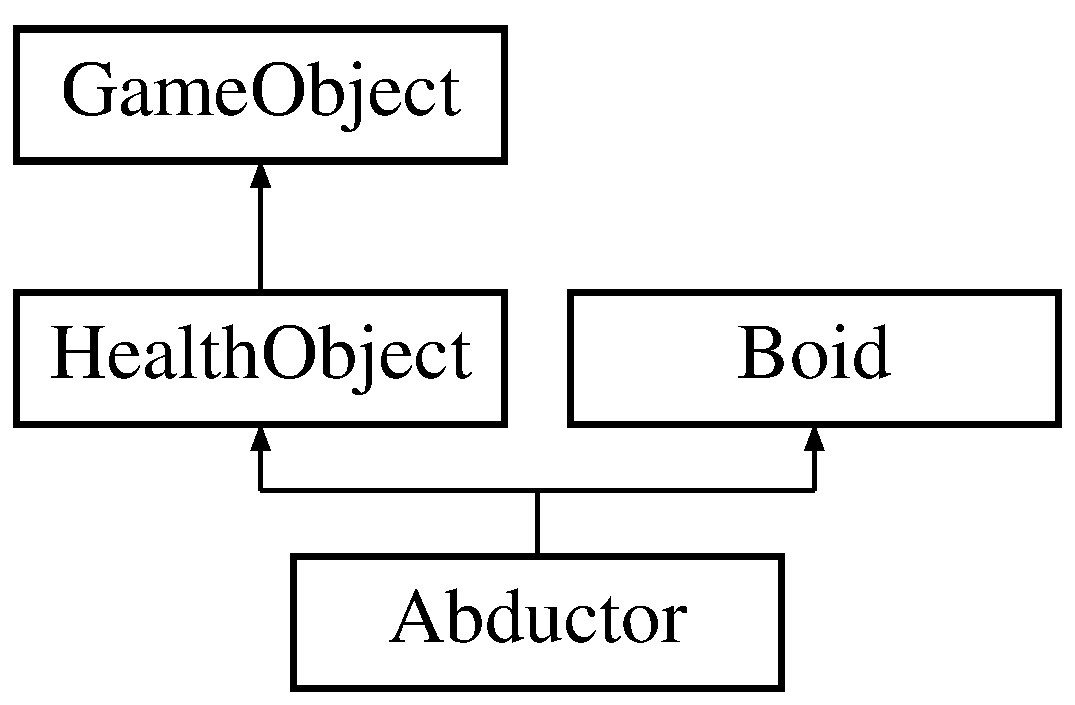
\includegraphics[height=3.000000cm]{class_abductor}
\end{center}
\end{figure}
\subsection*{Public Member Functions}
\begin{DoxyCompactItemize}
\item 
\hyperlink{class_abductor_ae0d55b9a8e855c02fe51fbb48613a4b7}{Abductor} (sf\+::\+Vector2f position, sf\+::\+Vector2f size, float min\+Patrol\+Height, float max\+Patrol\+Height)
\item 
virtual \hyperlink{class_abductor_adc657b211a1b36c55db079caa10d9010}{$\sim$\+Abductor} ()
\item 
void \hyperlink{class_abductor_a16c030380d94caf386171cda40ed1eb8}{Update} (float dt) override
\item 
void \hyperlink{class_abductor_a81e65919dcbdf472395f946d110825b2}{Update\+Shooting} (float dt)
\item 
void \hyperlink{class_abductor_aee5fadabe89f51885e51a08d4a2d9889}{Update\+State} ()
\item 
void \hyperlink{class_abductor_ab27e1580f1a11d483d97f028deda7370}{Draw} (sf\+::\+Render\+Window \&window) override
\item 
void \hyperlink{class_abductor_a6c68ecc2673674040f87c2409d8505a1}{Draw\+With\+X\+Offset} (sf\+::\+Render\+Window \&window, float x\+Offset) override
\item 
void \hyperlink{class_abductor_a4623b394ad899b8df96b52e997fa5b03}{wrap\+Positions} (\hyperlink{class_camera}{Camera} \&cam)
\item 
void \hyperlink{class_abductor_a3d6281a8a4ab08f7a01e358aa6c0ca7f}{set\+Closest\+Astronaut} (\hyperlink{class_vector2_d}{Vector2D} position, \hyperlink{class_astronaut}{Astronaut} $\ast$a)
\item 
void \hyperlink{class_abductor_a13164f20159447e3e50629283c7cd32d}{drop\+Astronaut} ()
\item 
void \hyperlink{class_abductor_a0c9d8d1e2978f6b794de34568baa266e}{calculate\+Abduct\+Position} ()
\item 
\hyperlink{class_vector2_d}{Vector2D} \hyperlink{class_abductor_a9b01cf2a2870454fe621a7bc5a2828e5}{get\+Position} () override
\item 
\hyperlink{class_vector2_d}{Vector2D} \hyperlink{class_abductor_adb812ea046ef9fc984b5035c7fb6ce3f}{get\+Velocity} () override
\item 
bool \hyperlink{class_abductor_a3a22e52687c4f1b70eba475617fec3a4}{is\+Abducting} ()
\item 
bool \hyperlink{class_abductor_a76abe6a51994ef35787351c9cd49ba6c}{is\+Patrolling} ()
\item 
bool \hyperlink{class_abductor_ab862b53793f2722546e3e1be05bd546e}{is\+Predator} () override
\item 
bool \hyperlink{class_abductor_af50d368af0d068122b2755a238bebfb7}{should\+Transform} ()
\item 
void \hyperlink{class_abductor_a7a37f57eb3c873e8b944b4757d1d87cd}{destroy\+Electrics} ()
\item 
void \hyperlink{class_abductor_a8be0f01a614756f913acf032fa64f474}{set\+GroundY} (float y)
\item 
bool \hyperlink{class_abductor_ab54e8bd43da87e3328ccaab48cbc79bb}{is\+Under\+E\+MP} ()
\end{DoxyCompactItemize}
\subsection*{Additional Inherited Members}


\subsection{Constructor \& Destructor Documentation}
\hypertarget{class_abductor_ae0d55b9a8e855c02fe51fbb48613a4b7}{}\label{class_abductor_ae0d55b9a8e855c02fe51fbb48613a4b7} 
\index{Abductor@{Abductor}!Abductor@{Abductor}}
\index{Abductor@{Abductor}!Abductor@{Abductor}}
\subsubsection{\texorpdfstring{Abductor()}{Abductor()}}
{\footnotesize\ttfamily Abductor\+::\+Abductor (\begin{DoxyParamCaption}\item[{sf\+::\+Vector2f}]{position,  }\item[{sf\+::\+Vector2f}]{size,  }\item[{float}]{min\+Patrol\+Height,  }\item[{float}]{max\+Patrol\+Height }\end{DoxyParamCaption})}

\hypertarget{class_abductor_adc657b211a1b36c55db079caa10d9010}{}\label{class_abductor_adc657b211a1b36c55db079caa10d9010} 
\index{Abductor@{Abductor}!````~Abductor@{$\sim$\+Abductor}}
\index{````~Abductor@{$\sim$\+Abductor}!Abductor@{Abductor}}
\subsubsection{\texorpdfstring{$\sim$\+Abductor()}{~Abductor()}}
{\footnotesize\ttfamily Abductor\+::$\sim$\+Abductor (\begin{DoxyParamCaption}{ }\end{DoxyParamCaption})\hspace{0.3cm}{\ttfamily [virtual]}}



\subsection{Member Function Documentation}
\hypertarget{class_abductor_a0c9d8d1e2978f6b794de34568baa266e}{}\label{class_abductor_a0c9d8d1e2978f6b794de34568baa266e} 
\index{Abductor@{Abductor}!calculate\+Abduct\+Position@{calculate\+Abduct\+Position}}
\index{calculate\+Abduct\+Position@{calculate\+Abduct\+Position}!Abductor@{Abductor}}
\subsubsection{\texorpdfstring{calculate\+Abduct\+Position()}{calculateAbductPosition()}}
{\footnotesize\ttfamily void Abductor\+::calculate\+Abduct\+Position (\begin{DoxyParamCaption}{ }\end{DoxyParamCaption})}

\hypertarget{class_abductor_a7a37f57eb3c873e8b944b4757d1d87cd}{}\label{class_abductor_a7a37f57eb3c873e8b944b4757d1d87cd} 
\index{Abductor@{Abductor}!destroy\+Electrics@{destroy\+Electrics}}
\index{destroy\+Electrics@{destroy\+Electrics}!Abductor@{Abductor}}
\subsubsection{\texorpdfstring{destroy\+Electrics()}{destroyElectrics()}}
{\footnotesize\ttfamily void Abductor\+::destroy\+Electrics (\begin{DoxyParamCaption}{ }\end{DoxyParamCaption})}

\hypertarget{class_abductor_ab27e1580f1a11d483d97f028deda7370}{}\label{class_abductor_ab27e1580f1a11d483d97f028deda7370} 
\index{Abductor@{Abductor}!Draw@{Draw}}
\index{Draw@{Draw}!Abductor@{Abductor}}
\subsubsection{\texorpdfstring{Draw()}{Draw()}}
{\footnotesize\ttfamily void Abductor\+::\+Draw (\begin{DoxyParamCaption}\item[{sf\+::\+Render\+Window \&}]{window }\end{DoxyParamCaption})\hspace{0.3cm}{\ttfamily [override]}, {\ttfamily [virtual]}}



Implements \hyperlink{class_game_object_a0bd45eb831b3d0959eb498cad3e412ce}{Game\+Object}.

\hypertarget{class_abductor_a6c68ecc2673674040f87c2409d8505a1}{}\label{class_abductor_a6c68ecc2673674040f87c2409d8505a1} 
\index{Abductor@{Abductor}!Draw\+With\+X\+Offset@{Draw\+With\+X\+Offset}}
\index{Draw\+With\+X\+Offset@{Draw\+With\+X\+Offset}!Abductor@{Abductor}}
\subsubsection{\texorpdfstring{Draw\+With\+X\+Offset()}{DrawWithXOffset()}}
{\footnotesize\ttfamily void Abductor\+::\+Draw\+With\+X\+Offset (\begin{DoxyParamCaption}\item[{sf\+::\+Render\+Window \&}]{window,  }\item[{float}]{x\+Offset }\end{DoxyParamCaption})\hspace{0.3cm}{\ttfamily [override]}, {\ttfamily [virtual]}}



Implements \hyperlink{class_game_object_a8a3c07e92775fe00baa9e661fefb224e}{Game\+Object}.

\hypertarget{class_abductor_a13164f20159447e3e50629283c7cd32d}{}\label{class_abductor_a13164f20159447e3e50629283c7cd32d} 
\index{Abductor@{Abductor}!drop\+Astronaut@{drop\+Astronaut}}
\index{drop\+Astronaut@{drop\+Astronaut}!Abductor@{Abductor}}
\subsubsection{\texorpdfstring{drop\+Astronaut()}{dropAstronaut()}}
{\footnotesize\ttfamily void Abductor\+::drop\+Astronaut (\begin{DoxyParamCaption}{ }\end{DoxyParamCaption})}

\hypertarget{class_abductor_a9b01cf2a2870454fe621a7bc5a2828e5}{}\label{class_abductor_a9b01cf2a2870454fe621a7bc5a2828e5} 
\index{Abductor@{Abductor}!get\+Position@{get\+Position}}
\index{get\+Position@{get\+Position}!Abductor@{Abductor}}
\subsubsection{\texorpdfstring{get\+Position()}{getPosition()}}
{\footnotesize\ttfamily \hyperlink{class_vector2_d}{Vector2D} Abductor\+::get\+Position (\begin{DoxyParamCaption}{ }\end{DoxyParamCaption})\hspace{0.3cm}{\ttfamily [override]}, {\ttfamily [virtual]}}



Implements \hyperlink{class_boid_a32f7601f73e7a109bbd79d43b15d2272}{Boid}.

\hypertarget{class_abductor_adb812ea046ef9fc984b5035c7fb6ce3f}{}\label{class_abductor_adb812ea046ef9fc984b5035c7fb6ce3f} 
\index{Abductor@{Abductor}!get\+Velocity@{get\+Velocity}}
\index{get\+Velocity@{get\+Velocity}!Abductor@{Abductor}}
\subsubsection{\texorpdfstring{get\+Velocity()}{getVelocity()}}
{\footnotesize\ttfamily \hyperlink{class_vector2_d}{Vector2D} Abductor\+::get\+Velocity (\begin{DoxyParamCaption}{ }\end{DoxyParamCaption})\hspace{0.3cm}{\ttfamily [override]}, {\ttfamily [virtual]}}



Implements \hyperlink{class_boid_a58472dead1db1399b75090bf48184619}{Boid}.

\hypertarget{class_abductor_a3a22e52687c4f1b70eba475617fec3a4}{}\label{class_abductor_a3a22e52687c4f1b70eba475617fec3a4} 
\index{Abductor@{Abductor}!is\+Abducting@{is\+Abducting}}
\index{is\+Abducting@{is\+Abducting}!Abductor@{Abductor}}
\subsubsection{\texorpdfstring{is\+Abducting()}{isAbducting()}}
{\footnotesize\ttfamily bool Abductor\+::is\+Abducting (\begin{DoxyParamCaption}{ }\end{DoxyParamCaption})}

\hypertarget{class_abductor_a76abe6a51994ef35787351c9cd49ba6c}{}\label{class_abductor_a76abe6a51994ef35787351c9cd49ba6c} 
\index{Abductor@{Abductor}!is\+Patrolling@{is\+Patrolling}}
\index{is\+Patrolling@{is\+Patrolling}!Abductor@{Abductor}}
\subsubsection{\texorpdfstring{is\+Patrolling()}{isPatrolling()}}
{\footnotesize\ttfamily bool Abductor\+::is\+Patrolling (\begin{DoxyParamCaption}{ }\end{DoxyParamCaption})}

\hypertarget{class_abductor_ab862b53793f2722546e3e1be05bd546e}{}\label{class_abductor_ab862b53793f2722546e3e1be05bd546e} 
\index{Abductor@{Abductor}!is\+Predator@{is\+Predator}}
\index{is\+Predator@{is\+Predator}!Abductor@{Abductor}}
\subsubsection{\texorpdfstring{is\+Predator()}{isPredator()}}
{\footnotesize\ttfamily bool Abductor\+::is\+Predator (\begin{DoxyParamCaption}{ }\end{DoxyParamCaption})\hspace{0.3cm}{\ttfamily [override]}, {\ttfamily [virtual]}}



Implements \hyperlink{class_boid_afdc731ff7d6b7f471c202c191c4abf77}{Boid}.

\hypertarget{class_abductor_ab54e8bd43da87e3328ccaab48cbc79bb}{}\label{class_abductor_ab54e8bd43da87e3328ccaab48cbc79bb} 
\index{Abductor@{Abductor}!is\+Under\+E\+MP@{is\+Under\+E\+MP}}
\index{is\+Under\+E\+MP@{is\+Under\+E\+MP}!Abductor@{Abductor}}
\subsubsection{\texorpdfstring{is\+Under\+E\+M\+P()}{isUnderEMP()}}
{\footnotesize\ttfamily bool Abductor\+::is\+Under\+E\+MP (\begin{DoxyParamCaption}{ }\end{DoxyParamCaption})}

\hypertarget{class_abductor_a3d6281a8a4ab08f7a01e358aa6c0ca7f}{}\label{class_abductor_a3d6281a8a4ab08f7a01e358aa6c0ca7f} 
\index{Abductor@{Abductor}!set\+Closest\+Astronaut@{set\+Closest\+Astronaut}}
\index{set\+Closest\+Astronaut@{set\+Closest\+Astronaut}!Abductor@{Abductor}}
\subsubsection{\texorpdfstring{set\+Closest\+Astronaut()}{setClosestAstronaut()}}
{\footnotesize\ttfamily void Abductor\+::set\+Closest\+Astronaut (\begin{DoxyParamCaption}\item[{\hyperlink{class_vector2_d}{Vector2D}}]{position,  }\item[{\hyperlink{class_astronaut}{Astronaut} $\ast$}]{a }\end{DoxyParamCaption})}

\hypertarget{class_abductor_a8be0f01a614756f913acf032fa64f474}{}\label{class_abductor_a8be0f01a614756f913acf032fa64f474} 
\index{Abductor@{Abductor}!set\+GroundY@{set\+GroundY}}
\index{set\+GroundY@{set\+GroundY}!Abductor@{Abductor}}
\subsubsection{\texorpdfstring{set\+Ground\+Y()}{setGroundY()}}
{\footnotesize\ttfamily void Abductor\+::set\+GroundY (\begin{DoxyParamCaption}\item[{float}]{y }\end{DoxyParamCaption})}

\hypertarget{class_abductor_af50d368af0d068122b2755a238bebfb7}{}\label{class_abductor_af50d368af0d068122b2755a238bebfb7} 
\index{Abductor@{Abductor}!should\+Transform@{should\+Transform}}
\index{should\+Transform@{should\+Transform}!Abductor@{Abductor}}
\subsubsection{\texorpdfstring{should\+Transform()}{shouldTransform()}}
{\footnotesize\ttfamily bool Abductor\+::should\+Transform (\begin{DoxyParamCaption}{ }\end{DoxyParamCaption})}

\hypertarget{class_abductor_a16c030380d94caf386171cda40ed1eb8}{}\label{class_abductor_a16c030380d94caf386171cda40ed1eb8} 
\index{Abductor@{Abductor}!Update@{Update}}
\index{Update@{Update}!Abductor@{Abductor}}
\subsubsection{\texorpdfstring{Update()}{Update()}}
{\footnotesize\ttfamily void Abductor\+::\+Update (\begin{DoxyParamCaption}\item[{float}]{dt }\end{DoxyParamCaption})\hspace{0.3cm}{\ttfamily [override]}, {\ttfamily [virtual]}}



Implements \hyperlink{class_game_object_a93ed63df640deb516a020530e7f8e045}{Game\+Object}.

\hypertarget{class_abductor_a81e65919dcbdf472395f946d110825b2}{}\label{class_abductor_a81e65919dcbdf472395f946d110825b2} 
\index{Abductor@{Abductor}!Update\+Shooting@{Update\+Shooting}}
\index{Update\+Shooting@{Update\+Shooting}!Abductor@{Abductor}}
\subsubsection{\texorpdfstring{Update\+Shooting()}{UpdateShooting()}}
{\footnotesize\ttfamily void Abductor\+::\+Update\+Shooting (\begin{DoxyParamCaption}\item[{float}]{dt }\end{DoxyParamCaption})}

\hypertarget{class_abductor_aee5fadabe89f51885e51a08d4a2d9889}{}\label{class_abductor_aee5fadabe89f51885e51a08d4a2d9889} 
\index{Abductor@{Abductor}!Update\+State@{Update\+State}}
\index{Update\+State@{Update\+State}!Abductor@{Abductor}}
\subsubsection{\texorpdfstring{Update\+State()}{UpdateState()}}
{\footnotesize\ttfamily void Abductor\+::\+Update\+State (\begin{DoxyParamCaption}{ }\end{DoxyParamCaption})}

\hypertarget{class_abductor_a4623b394ad899b8df96b52e997fa5b03}{}\label{class_abductor_a4623b394ad899b8df96b52e997fa5b03} 
\index{Abductor@{Abductor}!wrap\+Positions@{wrap\+Positions}}
\index{wrap\+Positions@{wrap\+Positions}!Abductor@{Abductor}}
\subsubsection{\texorpdfstring{wrap\+Positions()}{wrapPositions()}}
{\footnotesize\ttfamily void Abductor\+::wrap\+Positions (\begin{DoxyParamCaption}\item[{\hyperlink{class_camera}{Camera} \&}]{cam }\end{DoxyParamCaption})\hspace{0.3cm}{\ttfamily [virtual]}}



Reimplemented from \hyperlink{class_game_object_a53b129d55688652e25e6515d80e669ca}{Game\+Object}.



The documentation for this class was generated from the following files\+:\begin{DoxyCompactItemize}
\item 
Console\+Application2/\hyperlink{_abductor_8h}{Abductor.\+h}\item 
Console\+Application2/\hyperlink{_abductor_8cpp}{Abductor.\+cpp}\end{DoxyCompactItemize}

\hypertarget{class_a_i_manager}{}\section{A\+I\+Manager Class Reference}
\label{class_a_i_manager}\index{A\+I\+Manager@{A\+I\+Manager}}


{\ttfamily \#include $<$A\+I\+Manager.\+h$>$}

\subsection*{Static Public Member Functions}
\begin{DoxyCompactItemize}
\item 
static void \hyperlink{class_a_i_manager_a9ac554c9d74432fe3ef74fedab936847}{initialize} (sf\+::\+Float\+Rect level\+Bounds)
\item 
static \hyperlink{class_vector2_d}{Vector2D} \hyperlink{class_a_i_manager_a5d0b2b08188e1e3ccf816480e70cd123}{Separation} (std\+::vector$<$ \hyperlink{class_boid}{Boid} $\ast$$>$ flock\+Objects, \hyperlink{class_vector2_d}{Vector2D} \&position, \hyperlink{class_vector2_d}{Vector2D} \&velocity, const float max\+Speed, const float max\+Acceleration, bool predator=false)
\item 
static \hyperlink{class_vector2_d}{Vector2D} \hyperlink{class_a_i_manager_afe3cf14648ae243d21f4cabaa8cc2ec1}{Alignment} (std\+::vector$<$ \hyperlink{class_boid}{Boid} $\ast$$>$ flock\+Objects, \hyperlink{class_vector2_d}{Vector2D} \&position, \hyperlink{class_vector2_d}{Vector2D} \&velocity, const float max\+Speed, const float max\+Acceleration)
\item 
static \hyperlink{class_vector2_d}{Vector2D} \hyperlink{class_a_i_manager_ae70e083ab30b71c15384f5bdb345b462}{Cohesion} (std\+::vector$<$ \hyperlink{class_boid}{Boid} $\ast$$>$ flock\+Objects, \hyperlink{class_vector2_d}{Vector2D} \&position, \hyperlink{class_vector2_d}{Vector2D} \&velocity, \hyperlink{class_vector2_d}{Vector2D} \&acceleration, const float max\+Speed, const float max\+Acceleration)
\item 
static \hyperlink{class_vector2_d}{Vector2D} \hyperlink{class_a_i_manager_a6fb60f6d1707822f1d692272467cc06e}{seek} (\hyperlink{class_vector2_d}{Vector2D} target, \hyperlink{class_vector2_d}{Vector2D} \&velocity, \hyperlink{class_vector2_d}{Vector2D} \&acceleration, const float max\+Speed, const float max\+Acceleration)
\item 
static void \hyperlink{class_a_i_manager_ac57a276bbab23a0db4aafe9392dea156}{flock} (\hyperlink{class_boid}{Boid} $\ast$b, \hyperlink{class_vector2_d}{Vector2D} \&acceleration, \hyperlink{class_vector2_d}{Vector2D} \&position, \hyperlink{class_vector2_d}{Vector2D} \&velocity, const float max\+Speed, const float max\+Acceleration, bool predator=false)
\item 
static void \hyperlink{class_a_i_manager_a69a2ee2acf0bc9a11370a2f2aa88e986}{swarm} (\hyperlink{class_boid}{Boid} $\ast$b, \hyperlink{class_vector2_d}{Vector2D} position, \hyperlink{class_vector2_d}{Vector2D} \&acceleration)
\item 
static void \hyperlink{class_a_i_manager_aaa175d0e5d024f0965e3acd2e53f4fbd}{process} ()
\item 
static void \hyperlink{class_a_i_manager_a2154de38a09bfcd16ddc202c56467b0b}{register\+Player} (\hyperlink{class_player}{Player} $\ast$player)
\item 
static void \hyperlink{class_a_i_manager_a254b2cb95e86b6056c7625782f846a83}{register\+Abductor} (\hyperlink{class_abductor}{Abductor} $\ast$abductor)
\item 
static void \hyperlink{class_a_i_manager_af4c426ea6624b3fddebae90b38e60f8e}{register\+Astronaut} (\hyperlink{class_astronaut}{Astronaut} $\ast$astronaut)
\item 
static void \hyperlink{class_a_i_manager_aef2cec33330d60136ce1a3c1fa6ddf3d}{register\+Meteor} (\hyperlink{class_meteor}{Meteor} $\ast$m)
\item 
static void \hyperlink{class_a_i_manager_ae95e3ce383599bba475efd56c1659e8c}{unregister\+Meteor} (\hyperlink{class_meteor}{Meteor} $\ast$m)
\item 
static void \hyperlink{class_a_i_manager_ae76cc0872ad978e4a36ab41522bb1ea4}{register\+Swarm\+Boid} (\hyperlink{class_boid}{Boid} $\ast$b)
\item 
static void \hyperlink{class_a_i_manager_a5104415d465d8b6f73999cf5623b20a5}{register\+Flock\+Boid} (\hyperlink{class_boid}{Boid} $\ast$b)
\item 
static void \hyperlink{class_a_i_manager_accc5ec3be7c8df6f72aa519e47454a6d}{unregister\+Boid} (\hyperlink{class_boid}{Boid} $\ast$b)
\item 
static void \hyperlink{class_a_i_manager_a372acb15818c45e4f84848103d5afecf}{unregister\+Player} ()
\item 
static void \hyperlink{class_a_i_manager_a202fdf78a138904ef96a3a5b5ccbbe30}{unregister\+Astronaut} (\hyperlink{class_astronaut}{Astronaut} $\ast$astronaut)
\item 
static void \hyperlink{class_a_i_manager_a54dd2607612cbbfbfa4253e44645b74f}{avoid\+Obstacles} (\hyperlink{class_vector2_d}{Vector2D} m\+\_\+position, \hyperlink{class_vector2_d}{Vector2D} \&acceleration, const float M\+A\+X\+\_\+\+A\+C\+C\+EL)
\item 
static \hyperlink{class_vector2_d}{Vector2D} \hyperlink{class_a_i_manager_ae15963d08e5b13b33c44d2f018b7d53c}{get\+Player\+Pos} ()
\item 
static \hyperlink{class_vector2_d}{Vector2D} \hyperlink{class_a_i_manager_a1b2223e6059e0b5d303dbb1845ec252a}{get\+Closest\+Player\+Pos} (\hyperlink{class_vector2_d}{Vector2D} pos)
\item 
static void \hyperlink{class_a_i_manager_adac775408b1f5657948ac68876633ad6}{wander\+Thrust} (float dt, float \&time\+Until\+Decelerate, float M\+A\+X\+T\+I\+ME, \hyperlink{class_vector2_d}{Vector2D} \&velocity, \hyperlink{class_vector2_d}{Vector2D} \&acceleration, const float M\+A\+X\+\_\+\+A\+C\+C\+EL)
\item 
static void \hyperlink{class_a_i_manager_affdb0ecab44ebf429f5d8a3f08051416}{wander} (float dt, float \&time\+Remaining, int max\+Time, \hyperlink{class_vector2_d}{Vector2D} \&direction)
\item 
static void \hyperlink{class_a_i_manager_a130f5f0727fd01841265946e533de685}{wander\+Horizontal} (float dt, float \&time\+Remaining, int max\+Time, \hyperlink{class_vector2_d}{Vector2D} \&direction)
\item 
static void \hyperlink{class_a_i_manager_af83d3d5dc2b853811b92c463a88e434f}{seek\+Toward} (\hyperlink{class_vector2_d}{Vector2D} position, \hyperlink{class_vector2_d}{Vector2D} target\+Position, \hyperlink{class_vector2_d}{Vector2D} \&direction)
\item 
static void \hyperlink{class_a_i_manager_a9b04dd523dfb195990b365bacfcd1e92}{evade\+From} (\hyperlink{class_vector2_d}{Vector2D} position, \hyperlink{class_vector2_d}{Vector2D} target\+Position, \hyperlink{class_vector2_d}{Vector2D} \&direction)
\item 
static void \hyperlink{class_a_i_manager_ad4c0ad994de9e3d1a4780dd4050da257}{avoid} (\hyperlink{class_vector2_d}{Vector2D} position, \hyperlink{class_vector2_d}{Vector2D} target\+Position, \hyperlink{class_vector2_d}{Vector2D} \&acceleration, const float max\+Accel)
\item 
static void \hyperlink{class_a_i_manager_a96ee060f8e8d6f01280c2eff2d66ea6a}{jump\+To\+Random\+Position} (\hyperlink{class_vector2_d}{Vector2D} \&position)
\end{DoxyCompactItemize}


\subsection{Member Function Documentation}
\hypertarget{class_a_i_manager_afe3cf14648ae243d21f4cabaa8cc2ec1}{}\label{class_a_i_manager_afe3cf14648ae243d21f4cabaa8cc2ec1} 
\index{A\+I\+Manager@{A\+I\+Manager}!Alignment@{Alignment}}
\index{Alignment@{Alignment}!A\+I\+Manager@{A\+I\+Manager}}
\subsubsection{\texorpdfstring{Alignment()}{Alignment()}}
{\footnotesize\ttfamily \hyperlink{class_vector2_d}{Vector2D} A\+I\+Manager\+::\+Alignment (\begin{DoxyParamCaption}\item[{std\+::vector$<$ \hyperlink{class_boid}{Boid} $\ast$$>$}]{flock\+Objects,  }\item[{\hyperlink{class_vector2_d}{Vector2D} \&}]{position,  }\item[{\hyperlink{class_vector2_d}{Vector2D} \&}]{velocity,  }\item[{const float}]{max\+Speed,  }\item[{const float}]{max\+Acceleration }\end{DoxyParamCaption})\hspace{0.3cm}{\ttfamily [static]}}

\hypertarget{class_a_i_manager_ad4c0ad994de9e3d1a4780dd4050da257}{}\label{class_a_i_manager_ad4c0ad994de9e3d1a4780dd4050da257} 
\index{A\+I\+Manager@{A\+I\+Manager}!avoid@{avoid}}
\index{avoid@{avoid}!A\+I\+Manager@{A\+I\+Manager}}
\subsubsection{\texorpdfstring{avoid()}{avoid()}}
{\footnotesize\ttfamily void A\+I\+Manager\+::avoid (\begin{DoxyParamCaption}\item[{\hyperlink{class_vector2_d}{Vector2D}}]{position,  }\item[{\hyperlink{class_vector2_d}{Vector2D}}]{target\+Position,  }\item[{\hyperlink{class_vector2_d}{Vector2D} \&}]{acceleration,  }\item[{const float}]{max\+Accel }\end{DoxyParamCaption})\hspace{0.3cm}{\ttfamily [static]}}

\hypertarget{class_a_i_manager_a54dd2607612cbbfbfa4253e44645b74f}{}\label{class_a_i_manager_a54dd2607612cbbfbfa4253e44645b74f} 
\index{A\+I\+Manager@{A\+I\+Manager}!avoid\+Obstacles@{avoid\+Obstacles}}
\index{avoid\+Obstacles@{avoid\+Obstacles}!A\+I\+Manager@{A\+I\+Manager}}
\subsubsection{\texorpdfstring{avoid\+Obstacles()}{avoidObstacles()}}
{\footnotesize\ttfamily void A\+I\+Manager\+::avoid\+Obstacles (\begin{DoxyParamCaption}\item[{\hyperlink{class_vector2_d}{Vector2D}}]{m\+\_\+position,  }\item[{\hyperlink{class_vector2_d}{Vector2D} \&}]{acceleration,  }\item[{const float}]{M\+A\+X\+\_\+\+A\+C\+C\+EL }\end{DoxyParamCaption})\hspace{0.3cm}{\ttfamily [static]}}

\hypertarget{class_a_i_manager_ae70e083ab30b71c15384f5bdb345b462}{}\label{class_a_i_manager_ae70e083ab30b71c15384f5bdb345b462} 
\index{A\+I\+Manager@{A\+I\+Manager}!Cohesion@{Cohesion}}
\index{Cohesion@{Cohesion}!A\+I\+Manager@{A\+I\+Manager}}
\subsubsection{\texorpdfstring{Cohesion()}{Cohesion()}}
{\footnotesize\ttfamily \hyperlink{class_vector2_d}{Vector2D} A\+I\+Manager\+::\+Cohesion (\begin{DoxyParamCaption}\item[{std\+::vector$<$ \hyperlink{class_boid}{Boid} $\ast$$>$}]{flock\+Objects,  }\item[{\hyperlink{class_vector2_d}{Vector2D} \&}]{position,  }\item[{\hyperlink{class_vector2_d}{Vector2D} \&}]{velocity,  }\item[{\hyperlink{class_vector2_d}{Vector2D} \&}]{acceleration,  }\item[{const float}]{max\+Speed,  }\item[{const float}]{max\+Acceleration }\end{DoxyParamCaption})\hspace{0.3cm}{\ttfamily [static]}}

\hypertarget{class_a_i_manager_a9b04dd523dfb195990b365bacfcd1e92}{}\label{class_a_i_manager_a9b04dd523dfb195990b365bacfcd1e92} 
\index{A\+I\+Manager@{A\+I\+Manager}!evade\+From@{evade\+From}}
\index{evade\+From@{evade\+From}!A\+I\+Manager@{A\+I\+Manager}}
\subsubsection{\texorpdfstring{evade\+From()}{evadeFrom()}}
{\footnotesize\ttfamily void A\+I\+Manager\+::evade\+From (\begin{DoxyParamCaption}\item[{\hyperlink{class_vector2_d}{Vector2D}}]{position,  }\item[{\hyperlink{class_vector2_d}{Vector2D}}]{target\+Position,  }\item[{\hyperlink{class_vector2_d}{Vector2D} \&}]{direction }\end{DoxyParamCaption})\hspace{0.3cm}{\ttfamily [static]}}

\hypertarget{class_a_i_manager_ac57a276bbab23a0db4aafe9392dea156}{}\label{class_a_i_manager_ac57a276bbab23a0db4aafe9392dea156} 
\index{A\+I\+Manager@{A\+I\+Manager}!flock@{flock}}
\index{flock@{flock}!A\+I\+Manager@{A\+I\+Manager}}
\subsubsection{\texorpdfstring{flock()}{flock()}}
{\footnotesize\ttfamily void A\+I\+Manager\+::flock (\begin{DoxyParamCaption}\item[{\hyperlink{class_boid}{Boid} $\ast$}]{b,  }\item[{\hyperlink{class_vector2_d}{Vector2D} \&}]{acceleration,  }\item[{\hyperlink{class_vector2_d}{Vector2D} \&}]{position,  }\item[{\hyperlink{class_vector2_d}{Vector2D} \&}]{velocity,  }\item[{const float}]{max\+Speed,  }\item[{const float}]{max\+Acceleration,  }\item[{bool}]{predator = {\ttfamily false} }\end{DoxyParamCaption})\hspace{0.3cm}{\ttfamily [static]}}

\hypertarget{class_a_i_manager_a1b2223e6059e0b5d303dbb1845ec252a}{}\label{class_a_i_manager_a1b2223e6059e0b5d303dbb1845ec252a} 
\index{A\+I\+Manager@{A\+I\+Manager}!get\+Closest\+Player\+Pos@{get\+Closest\+Player\+Pos}}
\index{get\+Closest\+Player\+Pos@{get\+Closest\+Player\+Pos}!A\+I\+Manager@{A\+I\+Manager}}
\subsubsection{\texorpdfstring{get\+Closest\+Player\+Pos()}{getClosestPlayerPos()}}
{\footnotesize\ttfamily \hyperlink{class_vector2_d}{Vector2D} A\+I\+Manager\+::get\+Closest\+Player\+Pos (\begin{DoxyParamCaption}\item[{\hyperlink{class_vector2_d}{Vector2D}}]{pos }\end{DoxyParamCaption})\hspace{0.3cm}{\ttfamily [static]}}

\hypertarget{class_a_i_manager_ae15963d08e5b13b33c44d2f018b7d53c}{}\label{class_a_i_manager_ae15963d08e5b13b33c44d2f018b7d53c} 
\index{A\+I\+Manager@{A\+I\+Manager}!get\+Player\+Pos@{get\+Player\+Pos}}
\index{get\+Player\+Pos@{get\+Player\+Pos}!A\+I\+Manager@{A\+I\+Manager}}
\subsubsection{\texorpdfstring{get\+Player\+Pos()}{getPlayerPos()}}
{\footnotesize\ttfamily \hyperlink{class_vector2_d}{Vector2D} A\+I\+Manager\+::get\+Player\+Pos (\begin{DoxyParamCaption}{ }\end{DoxyParamCaption})\hspace{0.3cm}{\ttfamily [static]}}

\hypertarget{class_a_i_manager_a9ac554c9d74432fe3ef74fedab936847}{}\label{class_a_i_manager_a9ac554c9d74432fe3ef74fedab936847} 
\index{A\+I\+Manager@{A\+I\+Manager}!initialize@{initialize}}
\index{initialize@{initialize}!A\+I\+Manager@{A\+I\+Manager}}
\subsubsection{\texorpdfstring{initialize()}{initialize()}}
{\footnotesize\ttfamily void A\+I\+Manager\+::initialize (\begin{DoxyParamCaption}\item[{sf\+::\+Float\+Rect}]{level\+Bounds }\end{DoxyParamCaption})\hspace{0.3cm}{\ttfamily [static]}}

\hypertarget{class_a_i_manager_a96ee060f8e8d6f01280c2eff2d66ea6a}{}\label{class_a_i_manager_a96ee060f8e8d6f01280c2eff2d66ea6a} 
\index{A\+I\+Manager@{A\+I\+Manager}!jump\+To\+Random\+Position@{jump\+To\+Random\+Position}}
\index{jump\+To\+Random\+Position@{jump\+To\+Random\+Position}!A\+I\+Manager@{A\+I\+Manager}}
\subsubsection{\texorpdfstring{jump\+To\+Random\+Position()}{jumpToRandomPosition()}}
{\footnotesize\ttfamily void A\+I\+Manager\+::jump\+To\+Random\+Position (\begin{DoxyParamCaption}\item[{\hyperlink{class_vector2_d}{Vector2D} \&}]{position }\end{DoxyParamCaption})\hspace{0.3cm}{\ttfamily [static]}}

\hypertarget{class_a_i_manager_aaa175d0e5d024f0965e3acd2e53f4fbd}{}\label{class_a_i_manager_aaa175d0e5d024f0965e3acd2e53f4fbd} 
\index{A\+I\+Manager@{A\+I\+Manager}!process@{process}}
\index{process@{process}!A\+I\+Manager@{A\+I\+Manager}}
\subsubsection{\texorpdfstring{process()}{process()}}
{\footnotesize\ttfamily void A\+I\+Manager\+::process (\begin{DoxyParamCaption}{ }\end{DoxyParamCaption})\hspace{0.3cm}{\ttfamily [static]}}

\hypertarget{class_a_i_manager_a254b2cb95e86b6056c7625782f846a83}{}\label{class_a_i_manager_a254b2cb95e86b6056c7625782f846a83} 
\index{A\+I\+Manager@{A\+I\+Manager}!register\+Abductor@{register\+Abductor}}
\index{register\+Abductor@{register\+Abductor}!A\+I\+Manager@{A\+I\+Manager}}
\subsubsection{\texorpdfstring{register\+Abductor()}{registerAbductor()}}
{\footnotesize\ttfamily void A\+I\+Manager\+::register\+Abductor (\begin{DoxyParamCaption}\item[{\hyperlink{class_abductor}{Abductor} $\ast$}]{abductor }\end{DoxyParamCaption})\hspace{0.3cm}{\ttfamily [static]}}

\hypertarget{class_a_i_manager_af4c426ea6624b3fddebae90b38e60f8e}{}\label{class_a_i_manager_af4c426ea6624b3fddebae90b38e60f8e} 
\index{A\+I\+Manager@{A\+I\+Manager}!register\+Astronaut@{register\+Astronaut}}
\index{register\+Astronaut@{register\+Astronaut}!A\+I\+Manager@{A\+I\+Manager}}
\subsubsection{\texorpdfstring{register\+Astronaut()}{registerAstronaut()}}
{\footnotesize\ttfamily void A\+I\+Manager\+::register\+Astronaut (\begin{DoxyParamCaption}\item[{\hyperlink{class_astronaut}{Astronaut} $\ast$}]{astronaut }\end{DoxyParamCaption})\hspace{0.3cm}{\ttfamily [static]}}

\hypertarget{class_a_i_manager_a5104415d465d8b6f73999cf5623b20a5}{}\label{class_a_i_manager_a5104415d465d8b6f73999cf5623b20a5} 
\index{A\+I\+Manager@{A\+I\+Manager}!register\+Flock\+Boid@{register\+Flock\+Boid}}
\index{register\+Flock\+Boid@{register\+Flock\+Boid}!A\+I\+Manager@{A\+I\+Manager}}
\subsubsection{\texorpdfstring{register\+Flock\+Boid()}{registerFlockBoid()}}
{\footnotesize\ttfamily void A\+I\+Manager\+::register\+Flock\+Boid (\begin{DoxyParamCaption}\item[{\hyperlink{class_boid}{Boid} $\ast$}]{b }\end{DoxyParamCaption})\hspace{0.3cm}{\ttfamily [static]}}

\hypertarget{class_a_i_manager_aef2cec33330d60136ce1a3c1fa6ddf3d}{}\label{class_a_i_manager_aef2cec33330d60136ce1a3c1fa6ddf3d} 
\index{A\+I\+Manager@{A\+I\+Manager}!register\+Meteor@{register\+Meteor}}
\index{register\+Meteor@{register\+Meteor}!A\+I\+Manager@{A\+I\+Manager}}
\subsubsection{\texorpdfstring{register\+Meteor()}{registerMeteor()}}
{\footnotesize\ttfamily void A\+I\+Manager\+::register\+Meteor (\begin{DoxyParamCaption}\item[{\hyperlink{class_meteor}{Meteor} $\ast$}]{m }\end{DoxyParamCaption})\hspace{0.3cm}{\ttfamily [static]}}

\hypertarget{class_a_i_manager_a2154de38a09bfcd16ddc202c56467b0b}{}\label{class_a_i_manager_a2154de38a09bfcd16ddc202c56467b0b} 
\index{A\+I\+Manager@{A\+I\+Manager}!register\+Player@{register\+Player}}
\index{register\+Player@{register\+Player}!A\+I\+Manager@{A\+I\+Manager}}
\subsubsection{\texorpdfstring{register\+Player()}{registerPlayer()}}
{\footnotesize\ttfamily void A\+I\+Manager\+::register\+Player (\begin{DoxyParamCaption}\item[{\hyperlink{class_player}{Player} $\ast$}]{player }\end{DoxyParamCaption})\hspace{0.3cm}{\ttfamily [static]}}

\hypertarget{class_a_i_manager_ae76cc0872ad978e4a36ab41522bb1ea4}{}\label{class_a_i_manager_ae76cc0872ad978e4a36ab41522bb1ea4} 
\index{A\+I\+Manager@{A\+I\+Manager}!register\+Swarm\+Boid@{register\+Swarm\+Boid}}
\index{register\+Swarm\+Boid@{register\+Swarm\+Boid}!A\+I\+Manager@{A\+I\+Manager}}
\subsubsection{\texorpdfstring{register\+Swarm\+Boid()}{registerSwarmBoid()}}
{\footnotesize\ttfamily void A\+I\+Manager\+::register\+Swarm\+Boid (\begin{DoxyParamCaption}\item[{\hyperlink{class_boid}{Boid} $\ast$}]{b }\end{DoxyParamCaption})\hspace{0.3cm}{\ttfamily [static]}}

\hypertarget{class_a_i_manager_a6fb60f6d1707822f1d692272467cc06e}{}\label{class_a_i_manager_a6fb60f6d1707822f1d692272467cc06e} 
\index{A\+I\+Manager@{A\+I\+Manager}!seek@{seek}}
\index{seek@{seek}!A\+I\+Manager@{A\+I\+Manager}}
\subsubsection{\texorpdfstring{seek()}{seek()}}
{\footnotesize\ttfamily \hyperlink{class_vector2_d}{Vector2D} A\+I\+Manager\+::seek (\begin{DoxyParamCaption}\item[{\hyperlink{class_vector2_d}{Vector2D}}]{target,  }\item[{\hyperlink{class_vector2_d}{Vector2D} \&}]{velocity,  }\item[{\hyperlink{class_vector2_d}{Vector2D} \&}]{acceleration,  }\item[{const float}]{max\+Speed,  }\item[{const float}]{max\+Acceleration }\end{DoxyParamCaption})\hspace{0.3cm}{\ttfamily [static]}}

\hypertarget{class_a_i_manager_af83d3d5dc2b853811b92c463a88e434f}{}\label{class_a_i_manager_af83d3d5dc2b853811b92c463a88e434f} 
\index{A\+I\+Manager@{A\+I\+Manager}!seek\+Toward@{seek\+Toward}}
\index{seek\+Toward@{seek\+Toward}!A\+I\+Manager@{A\+I\+Manager}}
\subsubsection{\texorpdfstring{seek\+Toward()}{seekToward()}}
{\footnotesize\ttfamily void A\+I\+Manager\+::seek\+Toward (\begin{DoxyParamCaption}\item[{\hyperlink{class_vector2_d}{Vector2D}}]{position,  }\item[{\hyperlink{class_vector2_d}{Vector2D}}]{target\+Position,  }\item[{\hyperlink{class_vector2_d}{Vector2D} \&}]{direction }\end{DoxyParamCaption})\hspace{0.3cm}{\ttfamily [static]}}

\hypertarget{class_a_i_manager_a5d0b2b08188e1e3ccf816480e70cd123}{}\label{class_a_i_manager_a5d0b2b08188e1e3ccf816480e70cd123} 
\index{A\+I\+Manager@{A\+I\+Manager}!Separation@{Separation}}
\index{Separation@{Separation}!A\+I\+Manager@{A\+I\+Manager}}
\subsubsection{\texorpdfstring{Separation()}{Separation()}}
{\footnotesize\ttfamily \hyperlink{class_vector2_d}{Vector2D} A\+I\+Manager\+::\+Separation (\begin{DoxyParamCaption}\item[{std\+::vector$<$ \hyperlink{class_boid}{Boid} $\ast$$>$}]{flock\+Objects,  }\item[{\hyperlink{class_vector2_d}{Vector2D} \&}]{position,  }\item[{\hyperlink{class_vector2_d}{Vector2D} \&}]{velocity,  }\item[{const float}]{max\+Speed,  }\item[{const float}]{max\+Acceleration,  }\item[{bool}]{predator = {\ttfamily false} }\end{DoxyParamCaption})\hspace{0.3cm}{\ttfamily [static]}}

\hypertarget{class_a_i_manager_a69a2ee2acf0bc9a11370a2f2aa88e986}{}\label{class_a_i_manager_a69a2ee2acf0bc9a11370a2f2aa88e986} 
\index{A\+I\+Manager@{A\+I\+Manager}!swarm@{swarm}}
\index{swarm@{swarm}!A\+I\+Manager@{A\+I\+Manager}}
\subsubsection{\texorpdfstring{swarm()}{swarm()}}
{\footnotesize\ttfamily void A\+I\+Manager\+::swarm (\begin{DoxyParamCaption}\item[{\hyperlink{class_boid}{Boid} $\ast$}]{b,  }\item[{\hyperlink{class_vector2_d}{Vector2D}}]{position,  }\item[{\hyperlink{class_vector2_d}{Vector2D} \&}]{acceleration }\end{DoxyParamCaption})\hspace{0.3cm}{\ttfamily [static]}}

\hypertarget{class_a_i_manager_a202fdf78a138904ef96a3a5b5ccbbe30}{}\label{class_a_i_manager_a202fdf78a138904ef96a3a5b5ccbbe30} 
\index{A\+I\+Manager@{A\+I\+Manager}!unregister\+Astronaut@{unregister\+Astronaut}}
\index{unregister\+Astronaut@{unregister\+Astronaut}!A\+I\+Manager@{A\+I\+Manager}}
\subsubsection{\texorpdfstring{unregister\+Astronaut()}{unregisterAstronaut()}}
{\footnotesize\ttfamily void A\+I\+Manager\+::unregister\+Astronaut (\begin{DoxyParamCaption}\item[{\hyperlink{class_astronaut}{Astronaut} $\ast$}]{astronaut }\end{DoxyParamCaption})\hspace{0.3cm}{\ttfamily [static]}}

\hypertarget{class_a_i_manager_accc5ec3be7c8df6f72aa519e47454a6d}{}\label{class_a_i_manager_accc5ec3be7c8df6f72aa519e47454a6d} 
\index{A\+I\+Manager@{A\+I\+Manager}!unregister\+Boid@{unregister\+Boid}}
\index{unregister\+Boid@{unregister\+Boid}!A\+I\+Manager@{A\+I\+Manager}}
\subsubsection{\texorpdfstring{unregister\+Boid()}{unregisterBoid()}}
{\footnotesize\ttfamily void A\+I\+Manager\+::unregister\+Boid (\begin{DoxyParamCaption}\item[{\hyperlink{class_boid}{Boid} $\ast$}]{b }\end{DoxyParamCaption})\hspace{0.3cm}{\ttfamily [static]}}

\hypertarget{class_a_i_manager_ae95e3ce383599bba475efd56c1659e8c}{}\label{class_a_i_manager_ae95e3ce383599bba475efd56c1659e8c} 
\index{A\+I\+Manager@{A\+I\+Manager}!unregister\+Meteor@{unregister\+Meteor}}
\index{unregister\+Meteor@{unregister\+Meteor}!A\+I\+Manager@{A\+I\+Manager}}
\subsubsection{\texorpdfstring{unregister\+Meteor()}{unregisterMeteor()}}
{\footnotesize\ttfamily void A\+I\+Manager\+::unregister\+Meteor (\begin{DoxyParamCaption}\item[{\hyperlink{class_meteor}{Meteor} $\ast$}]{m }\end{DoxyParamCaption})\hspace{0.3cm}{\ttfamily [static]}}

\hypertarget{class_a_i_manager_a372acb15818c45e4f84848103d5afecf}{}\label{class_a_i_manager_a372acb15818c45e4f84848103d5afecf} 
\index{A\+I\+Manager@{A\+I\+Manager}!unregister\+Player@{unregister\+Player}}
\index{unregister\+Player@{unregister\+Player}!A\+I\+Manager@{A\+I\+Manager}}
\subsubsection{\texorpdfstring{unregister\+Player()}{unregisterPlayer()}}
{\footnotesize\ttfamily void A\+I\+Manager\+::unregister\+Player (\begin{DoxyParamCaption}{ }\end{DoxyParamCaption})\hspace{0.3cm}{\ttfamily [static]}}

\hypertarget{class_a_i_manager_affdb0ecab44ebf429f5d8a3f08051416}{}\label{class_a_i_manager_affdb0ecab44ebf429f5d8a3f08051416} 
\index{A\+I\+Manager@{A\+I\+Manager}!wander@{wander}}
\index{wander@{wander}!A\+I\+Manager@{A\+I\+Manager}}
\subsubsection{\texorpdfstring{wander()}{wander()}}
{\footnotesize\ttfamily void A\+I\+Manager\+::wander (\begin{DoxyParamCaption}\item[{float}]{dt,  }\item[{float \&}]{time\+Remaining,  }\item[{int}]{max\+Time,  }\item[{\hyperlink{class_vector2_d}{Vector2D} \&}]{direction }\end{DoxyParamCaption})\hspace{0.3cm}{\ttfamily [static]}}

\hypertarget{class_a_i_manager_a130f5f0727fd01841265946e533de685}{}\label{class_a_i_manager_a130f5f0727fd01841265946e533de685} 
\index{A\+I\+Manager@{A\+I\+Manager}!wander\+Horizontal@{wander\+Horizontal}}
\index{wander\+Horizontal@{wander\+Horizontal}!A\+I\+Manager@{A\+I\+Manager}}
\subsubsection{\texorpdfstring{wander\+Horizontal()}{wanderHorizontal()}}
{\footnotesize\ttfamily void A\+I\+Manager\+::wander\+Horizontal (\begin{DoxyParamCaption}\item[{float}]{dt,  }\item[{float \&}]{time\+Remaining,  }\item[{int}]{max\+Time,  }\item[{\hyperlink{class_vector2_d}{Vector2D} \&}]{direction }\end{DoxyParamCaption})\hspace{0.3cm}{\ttfamily [static]}}

\hypertarget{class_a_i_manager_adac775408b1f5657948ac68876633ad6}{}\label{class_a_i_manager_adac775408b1f5657948ac68876633ad6} 
\index{A\+I\+Manager@{A\+I\+Manager}!wander\+Thrust@{wander\+Thrust}}
\index{wander\+Thrust@{wander\+Thrust}!A\+I\+Manager@{A\+I\+Manager}}
\subsubsection{\texorpdfstring{wander\+Thrust()}{wanderThrust()}}
{\footnotesize\ttfamily void A\+I\+Manager\+::wander\+Thrust (\begin{DoxyParamCaption}\item[{float}]{dt,  }\item[{float \&}]{time\+Until\+Decelerate,  }\item[{float}]{M\+A\+X\+T\+I\+ME,  }\item[{\hyperlink{class_vector2_d}{Vector2D} \&}]{velocity,  }\item[{\hyperlink{class_vector2_d}{Vector2D} \&}]{acceleration,  }\item[{const float}]{M\+A\+X\+\_\+\+A\+C\+C\+EL }\end{DoxyParamCaption})\hspace{0.3cm}{\ttfamily [static]}}



The documentation for this class was generated from the following files\+:\begin{DoxyCompactItemize}
\item 
Console\+Application2/\hyperlink{_a_i_manager_8h}{A\+I\+Manager.\+h}\item 
Console\+Application2/\hyperlink{_a_i_manager_8cpp}{A\+I\+Manager.\+cpp}\end{DoxyCompactItemize}

\hypertarget{struct_asset}{}\section{Asset Struct Reference}
\label{struct_asset}\index{Asset@{Asset}}


{\ttfamily \#include $<$Asset.\+h$>$}

Inheritance diagram for Asset\+:\begin{figure}[H]
\begin{center}
\leavevmode
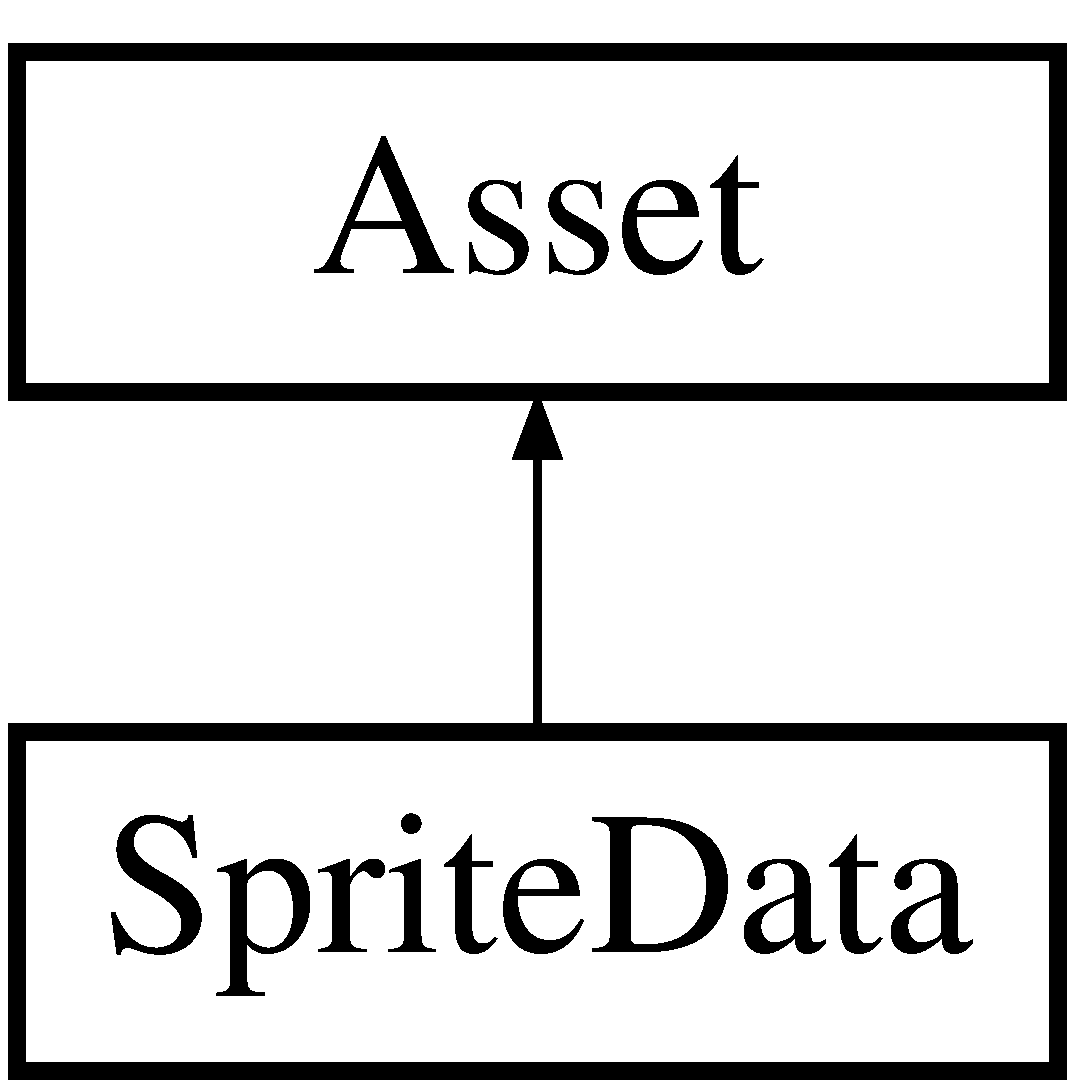
\includegraphics[height=2.000000cm]{struct_asset}
\end{center}
\end{figure}
\subsection*{Public Member Functions}
\begin{DoxyCompactItemize}
\item 
\hyperlink{struct_asset_ab6f3eef3374ddf89913a089e88683ccc}{Asset} (string key)
\item 
virtual string \hyperlink{struct_asset_acadc9dc60e4a89d711de110327df094c}{get\+Key} ()
\end{DoxyCompactItemize}
\subsection*{Protected Attributes}
\begin{DoxyCompactItemize}
\item 
string \hyperlink{struct_asset_abc299be0e567c1c57a545ddc12a2e9dc}{m\+\_\+key}
\end{DoxyCompactItemize}


\subsection{Constructor \& Destructor Documentation}
\hypertarget{struct_asset_ab6f3eef3374ddf89913a089e88683ccc}{}\label{struct_asset_ab6f3eef3374ddf89913a089e88683ccc} 
\index{Asset@{Asset}!Asset@{Asset}}
\index{Asset@{Asset}!Asset@{Asset}}
\subsubsection{\texorpdfstring{Asset()}{Asset()}}
{\footnotesize\ttfamily Asset\+::\+Asset (\begin{DoxyParamCaption}\item[{string}]{key }\end{DoxyParamCaption})\hspace{0.3cm}{\ttfamily [inline]}}



\subsection{Member Function Documentation}
\hypertarget{struct_asset_acadc9dc60e4a89d711de110327df094c}{}\label{struct_asset_acadc9dc60e4a89d711de110327df094c} 
\index{Asset@{Asset}!get\+Key@{get\+Key}}
\index{get\+Key@{get\+Key}!Asset@{Asset}}
\subsubsection{\texorpdfstring{get\+Key()}{getKey()}}
{\footnotesize\ttfamily virtual string Asset\+::get\+Key (\begin{DoxyParamCaption}{ }\end{DoxyParamCaption})\hspace{0.3cm}{\ttfamily [inline]}, {\ttfamily [virtual]}}



\subsection{Member Data Documentation}
\hypertarget{struct_asset_abc299be0e567c1c57a545ddc12a2e9dc}{}\label{struct_asset_abc299be0e567c1c57a545ddc12a2e9dc} 
\index{Asset@{Asset}!m\+\_\+key@{m\+\_\+key}}
\index{m\+\_\+key@{m\+\_\+key}!Asset@{Asset}}
\subsubsection{\texorpdfstring{m\+\_\+key}{m\_key}}
{\footnotesize\ttfamily string Asset\+::m\+\_\+key\hspace{0.3cm}{\ttfamily [protected]}}



The documentation for this struct was generated from the following file\+:\begin{DoxyCompactItemize}
\item 
Console\+Application2/\hyperlink{_asset_8h}{Asset.\+h}\end{DoxyCompactItemize}

\hypertarget{class_asset_loader}{}\section{Asset\+Loader Class Reference}
\label{class_asset_loader}\index{Asset\+Loader@{Asset\+Loader}}


{\ttfamily \#include $<$Asset\+Loader.\+h$>$}

\subsection*{Public Member Functions}
\begin{DoxyCompactItemize}
\item 
\hyperlink{class_asset_loader_a4f49d2d68ee1413e1f18dc7f4d003f0c}{$\sim$\+Asset\+Loader} ()
\item 
bool \hyperlink{class_asset_loader_a02606bccd43e16913919b3e081f74f3e}{exists} (string key)
\item 
void \hyperlink{class_asset_loader_a682bc76f35e281e4f6cf3d7b19388bbb}{empty\+Map} ()
\item 
void \hyperlink{class_asset_loader_ae902ff7d59878412699ae1dd5e3b1fc0}{add\+Texture\+To\+Cache} (string name, string \+\_\+texture\+File\+Path)
\item 
sf\+::\+Texture $\ast$ \hyperlink{class_asset_loader_a0f8159b836b5d23aadf4439cba9d5e84}{find\+Texture\+By\+Key} (string key)
\item 
void \hyperlink{class_asset_loader_ad5e2c8b9ad7ce00249f9ff5404d7363c}{load\+Textures} (string img\+Data\+Dir)
\item 
void \hyperlink{class_asset_loader_aaba5217d0cfe6203f3f47d3eb5dbe50c}{add\+Asset\+To\+Queue} (\hyperlink{struct_asset}{Asset} $\ast$asset)
\item 
void \hyperlink{class_asset_loader_a20c0aca89038b89980be63b7639c89ff}{load\+Asset\+Queue} ()
\item 
void \hyperlink{class_asset_loader_acf07e2074a4c86f3312d2c162ae5a40b}{load\+Asset} (\hyperlink{struct_asset}{Asset} $\ast$asset)
\item 
string \hyperlink{class_asset_loader_aa91b6dc15ed3f4befbd0c74bc1d7f040}{get\+Loading\+Asset} ()
\item 
int \hyperlink{class_asset_loader_a2b6e924a1ded0e1758a608757e6886fe}{get\+Num\+Loaded} ()
\item 
int \hyperlink{class_asset_loader_a5c122cf239d342643f38bb9dd3de7996}{get\+Num\+To\+Load} ()
\end{DoxyCompactItemize}
\subsection*{Static Public Member Functions}
\begin{DoxyCompactItemize}
\item 
static \hyperlink{class_asset_loader}{Asset\+Loader} $\ast$ \hyperlink{class_asset_loader_a84f304e93bb704447080e2e722e6d413}{get\+Instance} ()
\end{DoxyCompactItemize}
\subsection*{Protected Member Functions}
\begin{DoxyCompactItemize}
\item 
void \hyperlink{class_asset_loader_a02a029329bac26f078cc8a8248b484ad}{add\+To\+Image\+Cache} (string name, string \+\_\+texture\+File\+Path)
\item 
\hyperlink{class_asset_loader_ae090ac88a0e6df2c7cc560da9f4c4f25}{Asset\+Loader} ()
\end{DoxyCompactItemize}
\subsection*{Protected Attributes}
\begin{DoxyCompactItemize}
\item 
map$<$ string, sf\+::\+Texture $\ast$ $>$ \hyperlink{class_asset_loader_a1420f613835a3aa5ca97affb12b31da8}{image\+Cache}
\item 
vector$<$ \hyperlink{struct_asset}{Asset} $\ast$ $>$ \hyperlink{class_asset_loader_a9b8deb026e3b796b37c99cb1253d7868}{asset\+Queue}
\item 
int \hyperlink{class_asset_loader_a46d605269740622e52033a2d15f1041a}{m\+\_\+assets\+Loaded}
\item 
string \hyperlink{class_asset_loader_ad7816a644b0358ff24f308beb6c27b1e}{m\+\_\+current\+Asset}
\end{DoxyCompactItemize}
\subsection*{Static Protected Attributes}
\begin{DoxyCompactItemize}
\item 
static \hyperlink{class_asset_loader}{Asset\+Loader} $\ast$ \hyperlink{class_asset_loader_a8109777021214db1df6aace310c9f842}{instance} = nullptr
\end{DoxyCompactItemize}


\subsection{Constructor \& Destructor Documentation}
\hypertarget{class_asset_loader_a4f49d2d68ee1413e1f18dc7f4d003f0c}{}\label{class_asset_loader_a4f49d2d68ee1413e1f18dc7f4d003f0c} 
\index{Asset\+Loader@{Asset\+Loader}!````~Asset\+Loader@{$\sim$\+Asset\+Loader}}
\index{````~Asset\+Loader@{$\sim$\+Asset\+Loader}!Asset\+Loader@{Asset\+Loader}}
\subsubsection{\texorpdfstring{$\sim$\+Asset\+Loader()}{~AssetLoader()}}
{\footnotesize\ttfamily Asset\+Loader\+::$\sim$\+Asset\+Loader (\begin{DoxyParamCaption}{ }\end{DoxyParamCaption})}

\hypertarget{class_asset_loader_ae090ac88a0e6df2c7cc560da9f4c4f25}{}\label{class_asset_loader_ae090ac88a0e6df2c7cc560da9f4c4f25} 
\index{Asset\+Loader@{Asset\+Loader}!Asset\+Loader@{Asset\+Loader}}
\index{Asset\+Loader@{Asset\+Loader}!Asset\+Loader@{Asset\+Loader}}
\subsubsection{\texorpdfstring{Asset\+Loader()}{AssetLoader()}}
{\footnotesize\ttfamily Asset\+Loader\+::\+Asset\+Loader (\begin{DoxyParamCaption}{ }\end{DoxyParamCaption})\hspace{0.3cm}{\ttfamily [protected]}}



\subsection{Member Function Documentation}
\hypertarget{class_asset_loader_aaba5217d0cfe6203f3f47d3eb5dbe50c}{}\label{class_asset_loader_aaba5217d0cfe6203f3f47d3eb5dbe50c} 
\index{Asset\+Loader@{Asset\+Loader}!add\+Asset\+To\+Queue@{add\+Asset\+To\+Queue}}
\index{add\+Asset\+To\+Queue@{add\+Asset\+To\+Queue}!Asset\+Loader@{Asset\+Loader}}
\subsubsection{\texorpdfstring{add\+Asset\+To\+Queue()}{addAssetToQueue()}}
{\footnotesize\ttfamily void Asset\+Loader\+::add\+Asset\+To\+Queue (\begin{DoxyParamCaption}\item[{\hyperlink{struct_asset}{Asset} $\ast$}]{asset }\end{DoxyParamCaption})}

\hypertarget{class_asset_loader_ae902ff7d59878412699ae1dd5e3b1fc0}{}\label{class_asset_loader_ae902ff7d59878412699ae1dd5e3b1fc0} 
\index{Asset\+Loader@{Asset\+Loader}!add\+Texture\+To\+Cache@{add\+Texture\+To\+Cache}}
\index{add\+Texture\+To\+Cache@{add\+Texture\+To\+Cache}!Asset\+Loader@{Asset\+Loader}}
\subsubsection{\texorpdfstring{add\+Texture\+To\+Cache()}{addTextureToCache()}}
{\footnotesize\ttfamily void Asset\+Loader\+::add\+Texture\+To\+Cache (\begin{DoxyParamCaption}\item[{string}]{name,  }\item[{string}]{\+\_\+texture\+File\+Path }\end{DoxyParamCaption})}

\hypertarget{class_asset_loader_a02a029329bac26f078cc8a8248b484ad}{}\label{class_asset_loader_a02a029329bac26f078cc8a8248b484ad} 
\index{Asset\+Loader@{Asset\+Loader}!add\+To\+Image\+Cache@{add\+To\+Image\+Cache}}
\index{add\+To\+Image\+Cache@{add\+To\+Image\+Cache}!Asset\+Loader@{Asset\+Loader}}
\subsubsection{\texorpdfstring{add\+To\+Image\+Cache()}{addToImageCache()}}
{\footnotesize\ttfamily void Asset\+Loader\+::add\+To\+Image\+Cache (\begin{DoxyParamCaption}\item[{string}]{name,  }\item[{string}]{\+\_\+texture\+File\+Path }\end{DoxyParamCaption})\hspace{0.3cm}{\ttfamily [protected]}}

\hypertarget{class_asset_loader_a682bc76f35e281e4f6cf3d7b19388bbb}{}\label{class_asset_loader_a682bc76f35e281e4f6cf3d7b19388bbb} 
\index{Asset\+Loader@{Asset\+Loader}!empty\+Map@{empty\+Map}}
\index{empty\+Map@{empty\+Map}!Asset\+Loader@{Asset\+Loader}}
\subsubsection{\texorpdfstring{empty\+Map()}{emptyMap()}}
{\footnotesize\ttfamily void Asset\+Loader\+::empty\+Map (\begin{DoxyParamCaption}{ }\end{DoxyParamCaption})}

\hypertarget{class_asset_loader_a02606bccd43e16913919b3e081f74f3e}{}\label{class_asset_loader_a02606bccd43e16913919b3e081f74f3e} 
\index{Asset\+Loader@{Asset\+Loader}!exists@{exists}}
\index{exists@{exists}!Asset\+Loader@{Asset\+Loader}}
\subsubsection{\texorpdfstring{exists()}{exists()}}
{\footnotesize\ttfamily bool Asset\+Loader\+::exists (\begin{DoxyParamCaption}\item[{string}]{key }\end{DoxyParamCaption})}

\hypertarget{class_asset_loader_a0f8159b836b5d23aadf4439cba9d5e84}{}\label{class_asset_loader_a0f8159b836b5d23aadf4439cba9d5e84} 
\index{Asset\+Loader@{Asset\+Loader}!find\+Texture\+By\+Key@{find\+Texture\+By\+Key}}
\index{find\+Texture\+By\+Key@{find\+Texture\+By\+Key}!Asset\+Loader@{Asset\+Loader}}
\subsubsection{\texorpdfstring{find\+Texture\+By\+Key()}{findTextureByKey()}}
{\footnotesize\ttfamily sf\+::\+Texture $\ast$ Asset\+Loader\+::find\+Texture\+By\+Key (\begin{DoxyParamCaption}\item[{string}]{key }\end{DoxyParamCaption})}

\hypertarget{class_asset_loader_a84f304e93bb704447080e2e722e6d413}{}\label{class_asset_loader_a84f304e93bb704447080e2e722e6d413} 
\index{Asset\+Loader@{Asset\+Loader}!get\+Instance@{get\+Instance}}
\index{get\+Instance@{get\+Instance}!Asset\+Loader@{Asset\+Loader}}
\subsubsection{\texorpdfstring{get\+Instance()}{getInstance()}}
{\footnotesize\ttfamily \hyperlink{class_asset_loader}{Asset\+Loader} $\ast$ Asset\+Loader\+::get\+Instance (\begin{DoxyParamCaption}{ }\end{DoxyParamCaption})\hspace{0.3cm}{\ttfamily [static]}}

\hypertarget{class_asset_loader_aa91b6dc15ed3f4befbd0c74bc1d7f040}{}\label{class_asset_loader_aa91b6dc15ed3f4befbd0c74bc1d7f040} 
\index{Asset\+Loader@{Asset\+Loader}!get\+Loading\+Asset@{get\+Loading\+Asset}}
\index{get\+Loading\+Asset@{get\+Loading\+Asset}!Asset\+Loader@{Asset\+Loader}}
\subsubsection{\texorpdfstring{get\+Loading\+Asset()}{getLoadingAsset()}}
{\footnotesize\ttfamily string Asset\+Loader\+::get\+Loading\+Asset (\begin{DoxyParamCaption}{ }\end{DoxyParamCaption})}

\hypertarget{class_asset_loader_a2b6e924a1ded0e1758a608757e6886fe}{}\label{class_asset_loader_a2b6e924a1ded0e1758a608757e6886fe} 
\index{Asset\+Loader@{Asset\+Loader}!get\+Num\+Loaded@{get\+Num\+Loaded}}
\index{get\+Num\+Loaded@{get\+Num\+Loaded}!Asset\+Loader@{Asset\+Loader}}
\subsubsection{\texorpdfstring{get\+Num\+Loaded()}{getNumLoaded()}}
{\footnotesize\ttfamily int Asset\+Loader\+::get\+Num\+Loaded (\begin{DoxyParamCaption}{ }\end{DoxyParamCaption})}

\hypertarget{class_asset_loader_a5c122cf239d342643f38bb9dd3de7996}{}\label{class_asset_loader_a5c122cf239d342643f38bb9dd3de7996} 
\index{Asset\+Loader@{Asset\+Loader}!get\+Num\+To\+Load@{get\+Num\+To\+Load}}
\index{get\+Num\+To\+Load@{get\+Num\+To\+Load}!Asset\+Loader@{Asset\+Loader}}
\subsubsection{\texorpdfstring{get\+Num\+To\+Load()}{getNumToLoad()}}
{\footnotesize\ttfamily int Asset\+Loader\+::get\+Num\+To\+Load (\begin{DoxyParamCaption}{ }\end{DoxyParamCaption})}

\hypertarget{class_asset_loader_acf07e2074a4c86f3312d2c162ae5a40b}{}\label{class_asset_loader_acf07e2074a4c86f3312d2c162ae5a40b} 
\index{Asset\+Loader@{Asset\+Loader}!load\+Asset@{load\+Asset}}
\index{load\+Asset@{load\+Asset}!Asset\+Loader@{Asset\+Loader}}
\subsubsection{\texorpdfstring{load\+Asset()}{loadAsset()}}
{\footnotesize\ttfamily void Asset\+Loader\+::load\+Asset (\begin{DoxyParamCaption}\item[{\hyperlink{struct_asset}{Asset} $\ast$}]{asset }\end{DoxyParamCaption})}

\hypertarget{class_asset_loader_a20c0aca89038b89980be63b7639c89ff}{}\label{class_asset_loader_a20c0aca89038b89980be63b7639c89ff} 
\index{Asset\+Loader@{Asset\+Loader}!load\+Asset\+Queue@{load\+Asset\+Queue}}
\index{load\+Asset\+Queue@{load\+Asset\+Queue}!Asset\+Loader@{Asset\+Loader}}
\subsubsection{\texorpdfstring{load\+Asset\+Queue()}{loadAssetQueue()}}
{\footnotesize\ttfamily void Asset\+Loader\+::load\+Asset\+Queue (\begin{DoxyParamCaption}{ }\end{DoxyParamCaption})}

\hypertarget{class_asset_loader_ad5e2c8b9ad7ce00249f9ff5404d7363c}{}\label{class_asset_loader_ad5e2c8b9ad7ce00249f9ff5404d7363c} 
\index{Asset\+Loader@{Asset\+Loader}!load\+Textures@{load\+Textures}}
\index{load\+Textures@{load\+Textures}!Asset\+Loader@{Asset\+Loader}}
\subsubsection{\texorpdfstring{load\+Textures()}{loadTextures()}}
{\footnotesize\ttfamily void Asset\+Loader\+::load\+Textures (\begin{DoxyParamCaption}\item[{string}]{img\+Data\+Dir }\end{DoxyParamCaption})}



\subsection{Member Data Documentation}
\hypertarget{class_asset_loader_a9b8deb026e3b796b37c99cb1253d7868}{}\label{class_asset_loader_a9b8deb026e3b796b37c99cb1253d7868} 
\index{Asset\+Loader@{Asset\+Loader}!asset\+Queue@{asset\+Queue}}
\index{asset\+Queue@{asset\+Queue}!Asset\+Loader@{Asset\+Loader}}
\subsubsection{\texorpdfstring{asset\+Queue}{assetQueue}}
{\footnotesize\ttfamily vector$<$\hyperlink{struct_asset}{Asset}$\ast$$>$ Asset\+Loader\+::asset\+Queue\hspace{0.3cm}{\ttfamily [protected]}}

\hypertarget{class_asset_loader_a1420f613835a3aa5ca97affb12b31da8}{}\label{class_asset_loader_a1420f613835a3aa5ca97affb12b31da8} 
\index{Asset\+Loader@{Asset\+Loader}!image\+Cache@{image\+Cache}}
\index{image\+Cache@{image\+Cache}!Asset\+Loader@{Asset\+Loader}}
\subsubsection{\texorpdfstring{image\+Cache}{imageCache}}
{\footnotesize\ttfamily map$<$string, sf\+::\+Texture $\ast$$>$ Asset\+Loader\+::image\+Cache\hspace{0.3cm}{\ttfamily [protected]}}

\hypertarget{class_asset_loader_a8109777021214db1df6aace310c9f842}{}\label{class_asset_loader_a8109777021214db1df6aace310c9f842} 
\index{Asset\+Loader@{Asset\+Loader}!instance@{instance}}
\index{instance@{instance}!Asset\+Loader@{Asset\+Loader}}
\subsubsection{\texorpdfstring{instance}{instance}}
{\footnotesize\ttfamily \hyperlink{class_asset_loader}{Asset\+Loader} $\ast$ Asset\+Loader\+::instance = nullptr\hspace{0.3cm}{\ttfamily [static]}, {\ttfamily [protected]}}

\hypertarget{class_asset_loader_a46d605269740622e52033a2d15f1041a}{}\label{class_asset_loader_a46d605269740622e52033a2d15f1041a} 
\index{Asset\+Loader@{Asset\+Loader}!m\+\_\+assets\+Loaded@{m\+\_\+assets\+Loaded}}
\index{m\+\_\+assets\+Loaded@{m\+\_\+assets\+Loaded}!Asset\+Loader@{Asset\+Loader}}
\subsubsection{\texorpdfstring{m\+\_\+assets\+Loaded}{m\_assetsLoaded}}
{\footnotesize\ttfamily int Asset\+Loader\+::m\+\_\+assets\+Loaded\hspace{0.3cm}{\ttfamily [protected]}}

\hypertarget{class_asset_loader_ad7816a644b0358ff24f308beb6c27b1e}{}\label{class_asset_loader_ad7816a644b0358ff24f308beb6c27b1e} 
\index{Asset\+Loader@{Asset\+Loader}!m\+\_\+current\+Asset@{m\+\_\+current\+Asset}}
\index{m\+\_\+current\+Asset@{m\+\_\+current\+Asset}!Asset\+Loader@{Asset\+Loader}}
\subsubsection{\texorpdfstring{m\+\_\+current\+Asset}{m\_currentAsset}}
{\footnotesize\ttfamily string Asset\+Loader\+::m\+\_\+current\+Asset\hspace{0.3cm}{\ttfamily [protected]}}



The documentation for this class was generated from the following files\+:\begin{DoxyCompactItemize}
\item 
Console\+Application2/\hyperlink{_asset_loader_8h}{Asset\+Loader.\+h}\item 
Console\+Application2/\hyperlink{_asset_loader_8cpp}{Asset\+Loader.\+cpp}\end{DoxyCompactItemize}

\hypertarget{class_astronaut}{}\section{Astronaut Class Reference}
\label{class_astronaut}\index{Astronaut@{Astronaut}}


{\ttfamily \#include $<$Astronaut.\+h$>$}

Inheritance diagram for Astronaut\+:\begin{figure}[H]
\begin{center}
\leavevmode
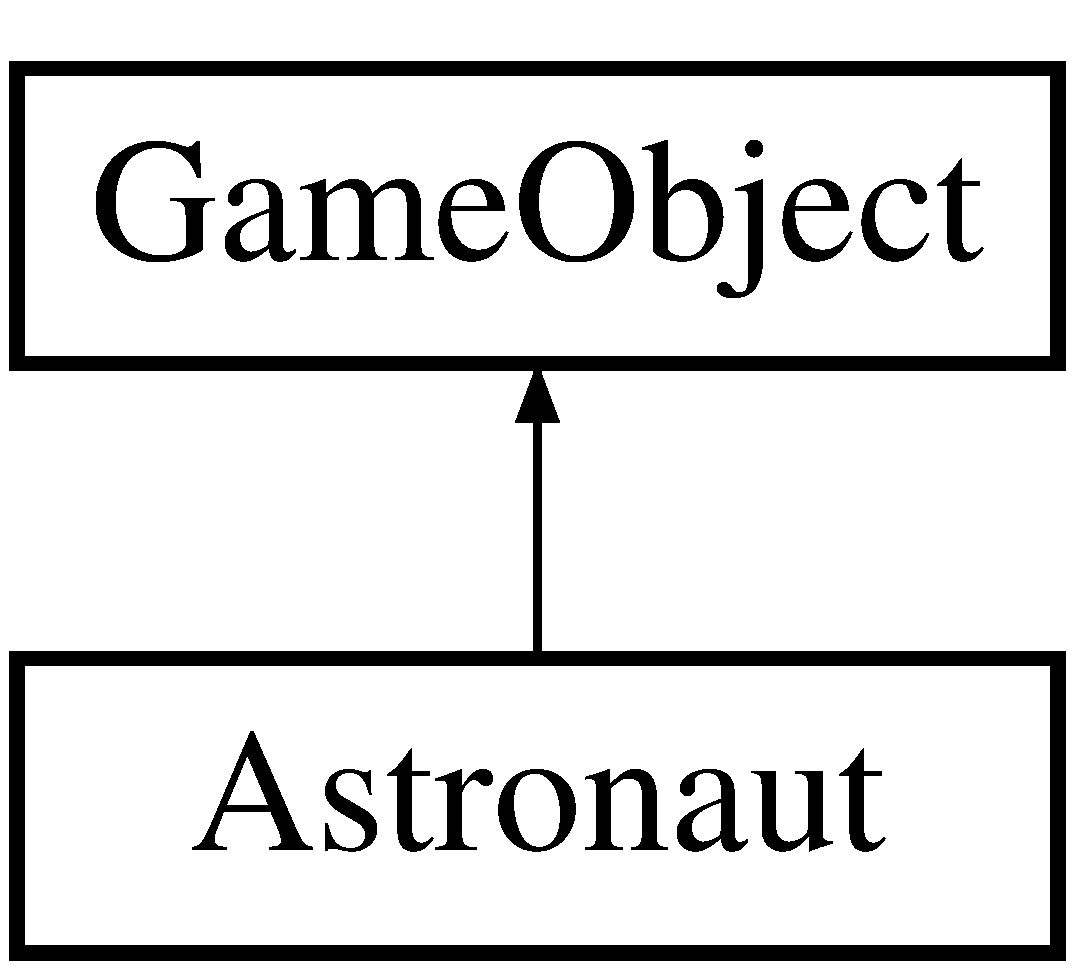
\includegraphics[height=2.000000cm]{class_astronaut}
\end{center}
\end{figure}
\subsection*{Public Member Functions}
\begin{DoxyCompactItemize}
\item 
\hyperlink{class_astronaut_a2c973afff53a1eca7b857b6d1dd8ba2f}{Astronaut} (sf\+::\+Vector2f position, sf\+::\+Vector2f size)
\item 
void \hyperlink{class_astronaut_a808e903cd53b5ce1e18c781ec06b1ead}{Update} (float dt) override
\item 
void \hyperlink{class_astronaut_a77c1d345c987d6d046642008a6f44343}{Update\+Position} (float dt)
\item 
void \hyperlink{class_astronaut_a574c4bb77cfb3f416ef1d51e54dca1f0}{Update\+State} ()
\item 
void \hyperlink{class_astronaut_ad87f989c99c64de938c367865cd196c4}{Draw} (sf\+::\+Render\+Window \&window) override
\item 
void \hyperlink{class_astronaut_ab37c4cce5348d86be1ec5ee652f5c917}{Draw\+With\+X\+Offset} (sf\+::\+Render\+Window \&window, float x\+Offset) override
\item 
void \hyperlink{class_astronaut_ab552db56a9d7341b3ce8f8a9b3670004}{wrap\+Positions} (\hyperlink{class_camera}{Camera} \&cam) override
\item 
\hyperlink{class_vector2_d}{Vector2D} \hyperlink{class_astronaut_a1d2ea689431e8aa1d783380b19115f7e}{get\+Position} ()
\item 
\hyperlink{class_vector2_d}{Vector2D} \hyperlink{class_astronaut_a6a526a639f9030f9638c845d90fbf3e4}{get\+Size} ()
\item 
void \hyperlink{class_astronaut_aa5cf10cf36c34114a8ecda156879cf80}{set\+Being\+Abducted} ()
\item 
void \hyperlink{class_astronaut_aca642a5da85bd7546c7750d87ffdad5c}{set\+Falling} ()
\item 
void \hyperlink{class_astronaut_a18df8dbedccb284469ad1f6e85948d3c}{set\+Closest\+Abductor} (\hyperlink{class_abductor}{Abductor} $\ast$abductor, \hyperlink{class_vector2_d}{Vector2D} position)
\item 
void \hyperlink{class_astronaut_afd8ed3067d597c58ab901a6d3cca2b40}{set\+Position} (\hyperlink{class_vector2_d}{Vector2D} position)
\item 
bool \hyperlink{class_astronaut_a1d7672f8b2d02bcb5bd25bd56b92c3b7}{is\+On\+Ground} ()
\end{DoxyCompactItemize}
\subsection*{Additional Inherited Members}


\subsection{Constructor \& Destructor Documentation}
\hypertarget{class_astronaut_a2c973afff53a1eca7b857b6d1dd8ba2f}{}\label{class_astronaut_a2c973afff53a1eca7b857b6d1dd8ba2f} 
\index{Astronaut@{Astronaut}!Astronaut@{Astronaut}}
\index{Astronaut@{Astronaut}!Astronaut@{Astronaut}}
\subsubsection{\texorpdfstring{Astronaut()}{Astronaut()}}
{\footnotesize\ttfamily Astronaut\+::\+Astronaut (\begin{DoxyParamCaption}\item[{sf\+::\+Vector2f}]{position,  }\item[{sf\+::\+Vector2f}]{size }\end{DoxyParamCaption})}



\subsection{Member Function Documentation}
\hypertarget{class_astronaut_ad87f989c99c64de938c367865cd196c4}{}\label{class_astronaut_ad87f989c99c64de938c367865cd196c4} 
\index{Astronaut@{Astronaut}!Draw@{Draw}}
\index{Draw@{Draw}!Astronaut@{Astronaut}}
\subsubsection{\texorpdfstring{Draw()}{Draw()}}
{\footnotesize\ttfamily void Astronaut\+::\+Draw (\begin{DoxyParamCaption}\item[{sf\+::\+Render\+Window \&}]{window }\end{DoxyParamCaption})\hspace{0.3cm}{\ttfamily [override]}, {\ttfamily [virtual]}}



Implements \hyperlink{class_game_object_a0bd45eb831b3d0959eb498cad3e412ce}{Game\+Object}.

\hypertarget{class_astronaut_ab37c4cce5348d86be1ec5ee652f5c917}{}\label{class_astronaut_ab37c4cce5348d86be1ec5ee652f5c917} 
\index{Astronaut@{Astronaut}!Draw\+With\+X\+Offset@{Draw\+With\+X\+Offset}}
\index{Draw\+With\+X\+Offset@{Draw\+With\+X\+Offset}!Astronaut@{Astronaut}}
\subsubsection{\texorpdfstring{Draw\+With\+X\+Offset()}{DrawWithXOffset()}}
{\footnotesize\ttfamily void Astronaut\+::\+Draw\+With\+X\+Offset (\begin{DoxyParamCaption}\item[{sf\+::\+Render\+Window \&}]{window,  }\item[{float}]{x\+Offset }\end{DoxyParamCaption})\hspace{0.3cm}{\ttfamily [override]}, {\ttfamily [virtual]}}



Implements \hyperlink{class_game_object_a8a3c07e92775fe00baa9e661fefb224e}{Game\+Object}.

\hypertarget{class_astronaut_a1d2ea689431e8aa1d783380b19115f7e}{}\label{class_astronaut_a1d2ea689431e8aa1d783380b19115f7e} 
\index{Astronaut@{Astronaut}!get\+Position@{get\+Position}}
\index{get\+Position@{get\+Position}!Astronaut@{Astronaut}}
\subsubsection{\texorpdfstring{get\+Position()}{getPosition()}}
{\footnotesize\ttfamily \hyperlink{class_vector2_d}{Vector2D} Astronaut\+::get\+Position (\begin{DoxyParamCaption}{ }\end{DoxyParamCaption})}

\hypertarget{class_astronaut_a6a526a639f9030f9638c845d90fbf3e4}{}\label{class_astronaut_a6a526a639f9030f9638c845d90fbf3e4} 
\index{Astronaut@{Astronaut}!get\+Size@{get\+Size}}
\index{get\+Size@{get\+Size}!Astronaut@{Astronaut}}
\subsubsection{\texorpdfstring{get\+Size()}{getSize()}}
{\footnotesize\ttfamily \hyperlink{class_vector2_d}{Vector2D} Astronaut\+::get\+Size (\begin{DoxyParamCaption}{ }\end{DoxyParamCaption})}

\hypertarget{class_astronaut_a1d7672f8b2d02bcb5bd25bd56b92c3b7}{}\label{class_astronaut_a1d7672f8b2d02bcb5bd25bd56b92c3b7} 
\index{Astronaut@{Astronaut}!is\+On\+Ground@{is\+On\+Ground}}
\index{is\+On\+Ground@{is\+On\+Ground}!Astronaut@{Astronaut}}
\subsubsection{\texorpdfstring{is\+On\+Ground()}{isOnGround()}}
{\footnotesize\ttfamily bool Astronaut\+::is\+On\+Ground (\begin{DoxyParamCaption}{ }\end{DoxyParamCaption})}

\hypertarget{class_astronaut_aa5cf10cf36c34114a8ecda156879cf80}{}\label{class_astronaut_aa5cf10cf36c34114a8ecda156879cf80} 
\index{Astronaut@{Astronaut}!set\+Being\+Abducted@{set\+Being\+Abducted}}
\index{set\+Being\+Abducted@{set\+Being\+Abducted}!Astronaut@{Astronaut}}
\subsubsection{\texorpdfstring{set\+Being\+Abducted()}{setBeingAbducted()}}
{\footnotesize\ttfamily void Astronaut\+::set\+Being\+Abducted (\begin{DoxyParamCaption}{ }\end{DoxyParamCaption})}

\hypertarget{class_astronaut_a18df8dbedccb284469ad1f6e85948d3c}{}\label{class_astronaut_a18df8dbedccb284469ad1f6e85948d3c} 
\index{Astronaut@{Astronaut}!set\+Closest\+Abductor@{set\+Closest\+Abductor}}
\index{set\+Closest\+Abductor@{set\+Closest\+Abductor}!Astronaut@{Astronaut}}
\subsubsection{\texorpdfstring{set\+Closest\+Abductor()}{setClosestAbductor()}}
{\footnotesize\ttfamily void Astronaut\+::set\+Closest\+Abductor (\begin{DoxyParamCaption}\item[{\hyperlink{class_abductor}{Abductor} $\ast$}]{abductor,  }\item[{\hyperlink{class_vector2_d}{Vector2D}}]{position }\end{DoxyParamCaption})}

\hypertarget{class_astronaut_aca642a5da85bd7546c7750d87ffdad5c}{}\label{class_astronaut_aca642a5da85bd7546c7750d87ffdad5c} 
\index{Astronaut@{Astronaut}!set\+Falling@{set\+Falling}}
\index{set\+Falling@{set\+Falling}!Astronaut@{Astronaut}}
\subsubsection{\texorpdfstring{set\+Falling()}{setFalling()}}
{\footnotesize\ttfamily void Astronaut\+::set\+Falling (\begin{DoxyParamCaption}{ }\end{DoxyParamCaption})}

\hypertarget{class_astronaut_afd8ed3067d597c58ab901a6d3cca2b40}{}\label{class_astronaut_afd8ed3067d597c58ab901a6d3cca2b40} 
\index{Astronaut@{Astronaut}!set\+Position@{set\+Position}}
\index{set\+Position@{set\+Position}!Astronaut@{Astronaut}}
\subsubsection{\texorpdfstring{set\+Position()}{setPosition()}}
{\footnotesize\ttfamily void Astronaut\+::set\+Position (\begin{DoxyParamCaption}\item[{\hyperlink{class_vector2_d}{Vector2D}}]{position }\end{DoxyParamCaption})}

\hypertarget{class_astronaut_a808e903cd53b5ce1e18c781ec06b1ead}{}\label{class_astronaut_a808e903cd53b5ce1e18c781ec06b1ead} 
\index{Astronaut@{Astronaut}!Update@{Update}}
\index{Update@{Update}!Astronaut@{Astronaut}}
\subsubsection{\texorpdfstring{Update()}{Update()}}
{\footnotesize\ttfamily void Astronaut\+::\+Update (\begin{DoxyParamCaption}\item[{float}]{dt }\end{DoxyParamCaption})\hspace{0.3cm}{\ttfamily [override]}, {\ttfamily [virtual]}}



Implements \hyperlink{class_game_object_a93ed63df640deb516a020530e7f8e045}{Game\+Object}.

\hypertarget{class_astronaut_a77c1d345c987d6d046642008a6f44343}{}\label{class_astronaut_a77c1d345c987d6d046642008a6f44343} 
\index{Astronaut@{Astronaut}!Update\+Position@{Update\+Position}}
\index{Update\+Position@{Update\+Position}!Astronaut@{Astronaut}}
\subsubsection{\texorpdfstring{Update\+Position()}{UpdatePosition()}}
{\footnotesize\ttfamily void Astronaut\+::\+Update\+Position (\begin{DoxyParamCaption}\item[{float}]{dt }\end{DoxyParamCaption})}

\hypertarget{class_astronaut_a574c4bb77cfb3f416ef1d51e54dca1f0}{}\label{class_astronaut_a574c4bb77cfb3f416ef1d51e54dca1f0} 
\index{Astronaut@{Astronaut}!Update\+State@{Update\+State}}
\index{Update\+State@{Update\+State}!Astronaut@{Astronaut}}
\subsubsection{\texorpdfstring{Update\+State()}{UpdateState()}}
{\footnotesize\ttfamily void Astronaut\+::\+Update\+State (\begin{DoxyParamCaption}{ }\end{DoxyParamCaption})}

\hypertarget{class_astronaut_ab552db56a9d7341b3ce8f8a9b3670004}{}\label{class_astronaut_ab552db56a9d7341b3ce8f8a9b3670004} 
\index{Astronaut@{Astronaut}!wrap\+Positions@{wrap\+Positions}}
\index{wrap\+Positions@{wrap\+Positions}!Astronaut@{Astronaut}}
\subsubsection{\texorpdfstring{wrap\+Positions()}{wrapPositions()}}
{\footnotesize\ttfamily void Astronaut\+::wrap\+Positions (\begin{DoxyParamCaption}\item[{\hyperlink{class_camera}{Camera} \&}]{cam }\end{DoxyParamCaption})\hspace{0.3cm}{\ttfamily [override]}, {\ttfamily [virtual]}}



Reimplemented from \hyperlink{class_game_object_a53b129d55688652e25e6515d80e669ca}{Game\+Object}.



The documentation for this class was generated from the following files\+:\begin{DoxyCompactItemize}
\item 
Console\+Application2/\hyperlink{_astronaut_8h}{Astronaut.\+h}\item 
Console\+Application2/\hyperlink{_astronaut_8cpp}{Astronaut.\+cpp}\end{DoxyCompactItemize}

\hypertarget{class_boid}{}\section{Boid Class Reference}
\label{class_boid}\index{Boid@{Boid}}


{\ttfamily \#include $<$Boid.\+h$>$}

Inheritance diagram for Boid\+:\begin{figure}[H]
\begin{center}
\leavevmode
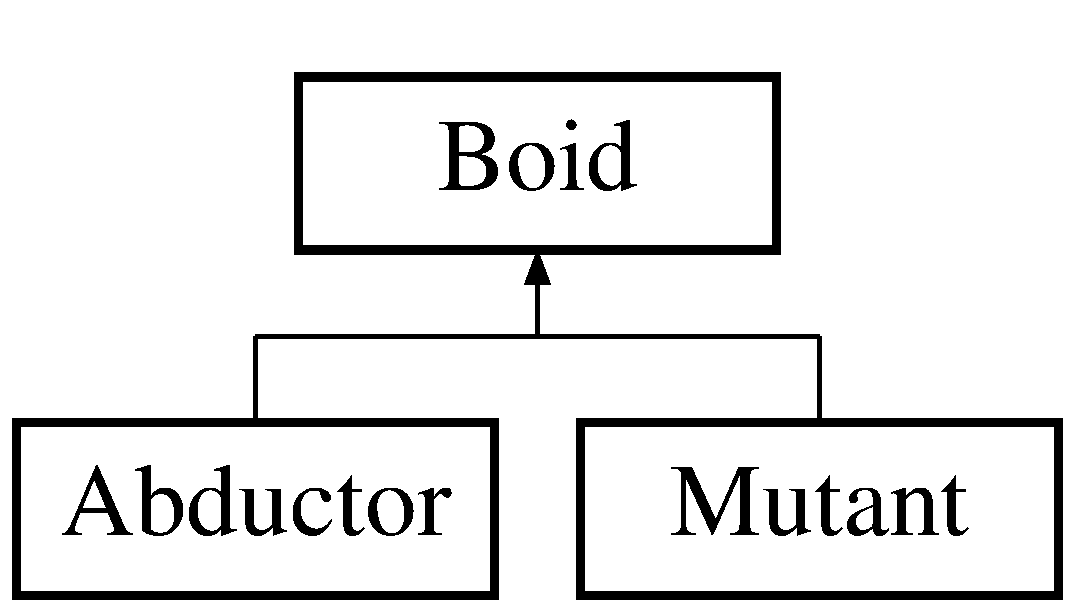
\includegraphics[height=2.000000cm]{class_boid}
\end{center}
\end{figure}
\subsection*{Public Member Functions}
\begin{DoxyCompactItemize}
\item 
\hyperlink{class_boid_ae8c6589e28ea9b0160e8403890ed2126}{Boid} (bool flocks)
\item 
virtual \hyperlink{class_vector2_d}{Vector2D} \hyperlink{class_boid_a32f7601f73e7a109bbd79d43b15d2272}{get\+Position} ()=0
\item 
virtual \hyperlink{class_vector2_d}{Vector2D} \hyperlink{class_boid_a58472dead1db1399b75090bf48184619}{get\+Velocity} ()=0
\item 
virtual bool \hyperlink{class_boid_afdc731ff7d6b7f471c202c191c4abf77}{is\+Predator} ()=0
\item 
virtual \hyperlink{class_boid_a712f84ddc1b8ad06ad7ecd6c10a1666c}{$\sim$\+Boid} ()
\end{DoxyCompactItemize}


\subsection{Constructor \& Destructor Documentation}
\hypertarget{class_boid_ae8c6589e28ea9b0160e8403890ed2126}{}\label{class_boid_ae8c6589e28ea9b0160e8403890ed2126} 
\index{Boid@{Boid}!Boid@{Boid}}
\index{Boid@{Boid}!Boid@{Boid}}
\subsubsection{\texorpdfstring{Boid()}{Boid()}}
{\footnotesize\ttfamily Boid\+::\+Boid (\begin{DoxyParamCaption}\item[{bool}]{flocks }\end{DoxyParamCaption})}

\hypertarget{class_boid_a712f84ddc1b8ad06ad7ecd6c10a1666c}{}\label{class_boid_a712f84ddc1b8ad06ad7ecd6c10a1666c} 
\index{Boid@{Boid}!````~Boid@{$\sim$\+Boid}}
\index{````~Boid@{$\sim$\+Boid}!Boid@{Boid}}
\subsubsection{\texorpdfstring{$\sim$\+Boid()}{~Boid()}}
{\footnotesize\ttfamily Boid\+::$\sim$\+Boid (\begin{DoxyParamCaption}{ }\end{DoxyParamCaption})\hspace{0.3cm}{\ttfamily [virtual]}}



\subsection{Member Function Documentation}
\hypertarget{class_boid_a32f7601f73e7a109bbd79d43b15d2272}{}\label{class_boid_a32f7601f73e7a109bbd79d43b15d2272} 
\index{Boid@{Boid}!get\+Position@{get\+Position}}
\index{get\+Position@{get\+Position}!Boid@{Boid}}
\subsubsection{\texorpdfstring{get\+Position()}{getPosition()}}
{\footnotesize\ttfamily virtual \hyperlink{class_vector2_d}{Vector2D} Boid\+::get\+Position (\begin{DoxyParamCaption}{ }\end{DoxyParamCaption})\hspace{0.3cm}{\ttfamily [pure virtual]}}



Implemented in \hyperlink{class_abductor_a9b01cf2a2870454fe621a7bc5a2828e5}{Abductor}, and \hyperlink{class_mutant_a9c3ab53037fc85159e02643ecfe46717}{Mutant}.

\hypertarget{class_boid_a58472dead1db1399b75090bf48184619}{}\label{class_boid_a58472dead1db1399b75090bf48184619} 
\index{Boid@{Boid}!get\+Velocity@{get\+Velocity}}
\index{get\+Velocity@{get\+Velocity}!Boid@{Boid}}
\subsubsection{\texorpdfstring{get\+Velocity()}{getVelocity()}}
{\footnotesize\ttfamily virtual \hyperlink{class_vector2_d}{Vector2D} Boid\+::get\+Velocity (\begin{DoxyParamCaption}{ }\end{DoxyParamCaption})\hspace{0.3cm}{\ttfamily [pure virtual]}}



Implemented in \hyperlink{class_abductor_adb812ea046ef9fc984b5035c7fb6ce3f}{Abductor}, and \hyperlink{class_mutant_af26928fa19102fe5ebea774819c4c565}{Mutant}.

\hypertarget{class_boid_afdc731ff7d6b7f471c202c191c4abf77}{}\label{class_boid_afdc731ff7d6b7f471c202c191c4abf77} 
\index{Boid@{Boid}!is\+Predator@{is\+Predator}}
\index{is\+Predator@{is\+Predator}!Boid@{Boid}}
\subsubsection{\texorpdfstring{is\+Predator()}{isPredator()}}
{\footnotesize\ttfamily virtual bool Boid\+::is\+Predator (\begin{DoxyParamCaption}{ }\end{DoxyParamCaption})\hspace{0.3cm}{\ttfamily [pure virtual]}}



Implemented in \hyperlink{class_abductor_ab862b53793f2722546e3e1be05bd546e}{Abductor}, and \hyperlink{class_mutant_a3416c1b42eb1e02bdcd4066109a28812}{Mutant}.



The documentation for this class was generated from the following files\+:\begin{DoxyCompactItemize}
\item 
Console\+Application2/\hyperlink{_boid_8h}{Boid.\+h}\item 
Console\+Application2/\hyperlink{_boid_8cpp}{Boid.\+cpp}\end{DoxyCompactItemize}

\hypertarget{class_bullet}{}\section{Bullet Class Reference}
\label{class_bullet}\index{Bullet@{Bullet}}


{\ttfamily \#include $<$Bullet.\+h$>$}

Inheritance diagram for Bullet\+:\begin{figure}[H]
\begin{center}
\leavevmode
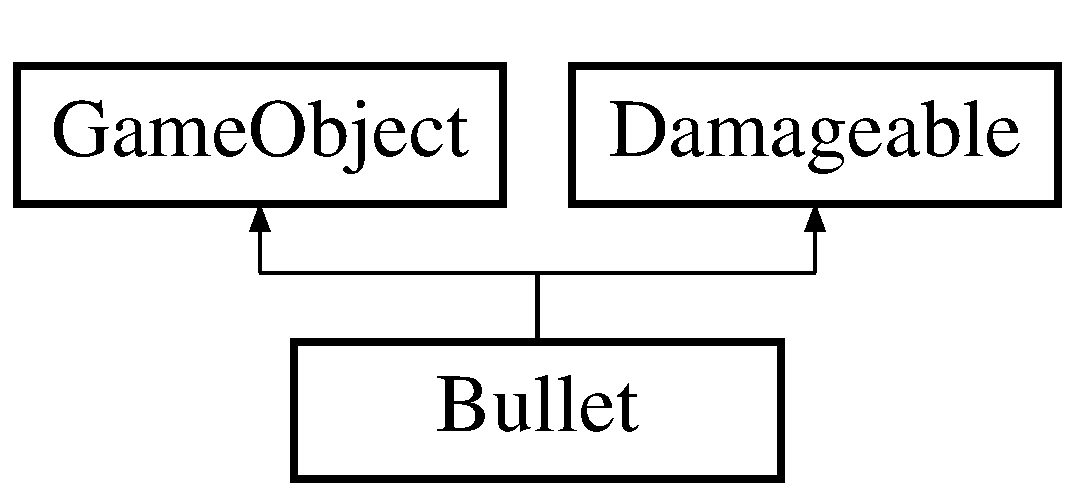
\includegraphics[height=2.000000cm]{class_bullet}
\end{center}
\end{figure}
\subsection*{Public Member Functions}
\begin{DoxyCompactItemize}
\item 
\hyperlink{class_bullet_ab64df756dc1c7f021eba572f0f621b10}{Bullet} (\hyperlink{class_vector2_d}{Vector2D} pos, \hyperlink{class_vector2_d}{Vector2D} dir)
\item 
\hyperlink{class_bullet_aaeb5cb41d7db89f49007b08b41f1bfcf}{$\sim$\+Bullet} ()
\item 
void \hyperlink{class_bullet_a539b6ae5c3e6ae431f097296371e8d31}{Update} (float dt) override
\item 
void \hyperlink{class_bullet_ac33e38185d1800e4a532c71a620d1bf7}{wrap\+Positions} (\hyperlink{class_camera}{Camera} \&cam) override
\item 
void \hyperlink{class_bullet_a44b861616d73fd5cd0fe78af2acda9c1}{Draw} (sf\+::\+Render\+Window \&w) override
\item 
void \hyperlink{class_bullet_ae3696edcf0c726c8c1b18a62faef8c03}{Draw\+With\+X\+Offset} (sf\+::\+Render\+Window \&window, float x\+Offset) override
\end{DoxyCompactItemize}
\subsection*{Additional Inherited Members}


\subsection{Constructor \& Destructor Documentation}
\hypertarget{class_bullet_ab64df756dc1c7f021eba572f0f621b10}{}\label{class_bullet_ab64df756dc1c7f021eba572f0f621b10} 
\index{Bullet@{Bullet}!Bullet@{Bullet}}
\index{Bullet@{Bullet}!Bullet@{Bullet}}
\subsubsection{\texorpdfstring{Bullet()}{Bullet()}}
{\footnotesize\ttfamily Bullet\+::\+Bullet (\begin{DoxyParamCaption}\item[{\hyperlink{class_vector2_d}{Vector2D}}]{pos,  }\item[{\hyperlink{class_vector2_d}{Vector2D}}]{dir }\end{DoxyParamCaption})}

\hypertarget{class_bullet_aaeb5cb41d7db89f49007b08b41f1bfcf}{}\label{class_bullet_aaeb5cb41d7db89f49007b08b41f1bfcf} 
\index{Bullet@{Bullet}!````~Bullet@{$\sim$\+Bullet}}
\index{````~Bullet@{$\sim$\+Bullet}!Bullet@{Bullet}}
\subsubsection{\texorpdfstring{$\sim$\+Bullet()}{~Bullet()}}
{\footnotesize\ttfamily Bullet\+::$\sim$\+Bullet (\begin{DoxyParamCaption}{ }\end{DoxyParamCaption})}



\subsection{Member Function Documentation}
\hypertarget{class_bullet_a44b861616d73fd5cd0fe78af2acda9c1}{}\label{class_bullet_a44b861616d73fd5cd0fe78af2acda9c1} 
\index{Bullet@{Bullet}!Draw@{Draw}}
\index{Draw@{Draw}!Bullet@{Bullet}}
\subsubsection{\texorpdfstring{Draw()}{Draw()}}
{\footnotesize\ttfamily void Bullet\+::\+Draw (\begin{DoxyParamCaption}\item[{sf\+::\+Render\+Window \&}]{w }\end{DoxyParamCaption})\hspace{0.3cm}{\ttfamily [override]}, {\ttfamily [virtual]}}



Implements \hyperlink{class_game_object_a0bd45eb831b3d0959eb498cad3e412ce}{Game\+Object}.

\hypertarget{class_bullet_ae3696edcf0c726c8c1b18a62faef8c03}{}\label{class_bullet_ae3696edcf0c726c8c1b18a62faef8c03} 
\index{Bullet@{Bullet}!Draw\+With\+X\+Offset@{Draw\+With\+X\+Offset}}
\index{Draw\+With\+X\+Offset@{Draw\+With\+X\+Offset}!Bullet@{Bullet}}
\subsubsection{\texorpdfstring{Draw\+With\+X\+Offset()}{DrawWithXOffset()}}
{\footnotesize\ttfamily void Bullet\+::\+Draw\+With\+X\+Offset (\begin{DoxyParamCaption}\item[{sf\+::\+Render\+Window \&}]{window,  }\item[{float}]{x\+Offset }\end{DoxyParamCaption})\hspace{0.3cm}{\ttfamily [override]}, {\ttfamily [virtual]}}



Implements \hyperlink{class_game_object_a8a3c07e92775fe00baa9e661fefb224e}{Game\+Object}.

\hypertarget{class_bullet_a539b6ae5c3e6ae431f097296371e8d31}{}\label{class_bullet_a539b6ae5c3e6ae431f097296371e8d31} 
\index{Bullet@{Bullet}!Update@{Update}}
\index{Update@{Update}!Bullet@{Bullet}}
\subsubsection{\texorpdfstring{Update()}{Update()}}
{\footnotesize\ttfamily void Bullet\+::\+Update (\begin{DoxyParamCaption}\item[{float}]{dt }\end{DoxyParamCaption})\hspace{0.3cm}{\ttfamily [override]}, {\ttfamily [virtual]}}



Implements \hyperlink{class_game_object_a93ed63df640deb516a020530e7f8e045}{Game\+Object}.

\hypertarget{class_bullet_ac33e38185d1800e4a532c71a620d1bf7}{}\label{class_bullet_ac33e38185d1800e4a532c71a620d1bf7} 
\index{Bullet@{Bullet}!wrap\+Positions@{wrap\+Positions}}
\index{wrap\+Positions@{wrap\+Positions}!Bullet@{Bullet}}
\subsubsection{\texorpdfstring{wrap\+Positions()}{wrapPositions()}}
{\footnotesize\ttfamily void Bullet\+::wrap\+Positions (\begin{DoxyParamCaption}\item[{\hyperlink{class_camera}{Camera} \&}]{cam }\end{DoxyParamCaption})\hspace{0.3cm}{\ttfamily [override]}, {\ttfamily [virtual]}}



Reimplemented from \hyperlink{class_game_object_a53b129d55688652e25e6515d80e669ca}{Game\+Object}.



The documentation for this class was generated from the following files\+:\begin{DoxyCompactItemize}
\item 
Console\+Application2/\hyperlink{_bullet_8h}{Bullet.\+h}\item 
Console\+Application2/\hyperlink{_bullet_8cpp}{Bullet.\+cpp}\end{DoxyCompactItemize}

\hypertarget{class_camera}{}\section{Camera Class Reference}
\label{class_camera}\index{Camera@{Camera}}


{\ttfamily \#include $<$Camera.\+h$>$}

\subsection*{Public Member Functions}
\begin{DoxyCompactItemize}
\item 
\hyperlink{class_camera_a52482616d4b8612775a639292303828d}{Camera} (\hyperlink{class_vector2_d}{Vector2D} screen\+Size, \hyperlink{class_vector2_d}{Vector2D} level\+Size)
\item 
void \hyperlink{class_camera_a2b7f120e90a5dc351ed44acf4af49729}{Move} (sf\+::\+Vector2f move\+Amount)
\item 
void \hyperlink{class_camera_a202fc4aff11dc17b8db71b5528c8476a}{Set\+Center} (sf\+::\+Vector2f center)
\item 
sf\+::\+Float\+Rect \hyperlink{class_camera_a77f821b5003fad8f5050ba802dd667e8}{get\+View\+Port} (sf\+::\+View \&v)
\item 
void \hyperlink{class_camera_a4795eceabe4768f35007dcb0083d418e}{Render\+Objects} (sf\+::\+Render\+Window \&window, std\+::vector$<$ \hyperlink{class_game_object}{Game\+Object} $\ast$$>$ \&m\+\_\+game\+Objects)
\item 
void \hyperlink{class_camera_a0b31de4a23f304be6e27d53706d326c5}{Update\+View} ()
\item 
void \hyperlink{class_camera_aadd889d41e7856d1c00609a7823c031f}{Render\+View} (sf\+::\+Render\+Window \&window, sf\+::\+View \&view, std\+::vector$<$ \hyperlink{class_game_object}{Game\+Object} $\ast$$>$ \&objects)
\item 
bool \hyperlink{class_camera_a8058d6b1c91c5d3ec5e410e5d0890737}{is\+A\+A\+B\+B\+In\+Viewport} (sf\+::\+Float\+Rect A\+A\+BB, sf\+::\+Float\+Rect viewport)
\item 
void \hyperlink{class_camera_aca617187658f1cea7f9633b4f62f1e93}{Wrap} (\hyperlink{class_vector2_d}{Vector2D} \&position)
\item 
void \hyperlink{class_camera_ad2f98f35c9a25c335ce7c5e6beae1ff9}{Wrap} (sf\+::\+Float\+Rect \&bounds)
\item 
std\+::vector$<$ \hyperlink{class_game_object}{Game\+Object} $\ast$ $>$ \hyperlink{class_camera_a8143cba00af1c4fca71d9597ebb0c748}{get\+Objects\+In\+View\+Port} (std\+::vector$<$ \hyperlink{class_game_object}{Game\+Object} $\ast$$>$ objects)
\end{DoxyCompactItemize}


\subsection{Constructor \& Destructor Documentation}
\hypertarget{class_camera_a52482616d4b8612775a639292303828d}{}\label{class_camera_a52482616d4b8612775a639292303828d} 
\index{Camera@{Camera}!Camera@{Camera}}
\index{Camera@{Camera}!Camera@{Camera}}
\subsubsection{\texorpdfstring{Camera()}{Camera()}}
{\footnotesize\ttfamily Camera\+::\+Camera (\begin{DoxyParamCaption}\item[{\hyperlink{class_vector2_d}{Vector2D}}]{screen\+Size,  }\item[{\hyperlink{class_vector2_d}{Vector2D}}]{level\+Size }\end{DoxyParamCaption})}



\subsection{Member Function Documentation}
\hypertarget{class_camera_a8143cba00af1c4fca71d9597ebb0c748}{}\label{class_camera_a8143cba00af1c4fca71d9597ebb0c748} 
\index{Camera@{Camera}!get\+Objects\+In\+View\+Port@{get\+Objects\+In\+View\+Port}}
\index{get\+Objects\+In\+View\+Port@{get\+Objects\+In\+View\+Port}!Camera@{Camera}}
\subsubsection{\texorpdfstring{get\+Objects\+In\+View\+Port()}{getObjectsInViewPort()}}
{\footnotesize\ttfamily std\+::vector$<$ \hyperlink{class_game_object}{Game\+Object} $\ast$ $>$ Camera\+::get\+Objects\+In\+View\+Port (\begin{DoxyParamCaption}\item[{std\+::vector$<$ \hyperlink{class_game_object}{Game\+Object} $\ast$$>$}]{objects }\end{DoxyParamCaption})}

\hypertarget{class_camera_a77f821b5003fad8f5050ba802dd667e8}{}\label{class_camera_a77f821b5003fad8f5050ba802dd667e8} 
\index{Camera@{Camera}!get\+View\+Port@{get\+View\+Port}}
\index{get\+View\+Port@{get\+View\+Port}!Camera@{Camera}}
\subsubsection{\texorpdfstring{get\+View\+Port()}{getViewPort()}}
{\footnotesize\ttfamily sf\+::\+Float\+Rect Camera\+::get\+View\+Port (\begin{DoxyParamCaption}\item[{sf\+::\+View \&}]{v }\end{DoxyParamCaption})}

\hypertarget{class_camera_a8058d6b1c91c5d3ec5e410e5d0890737}{}\label{class_camera_a8058d6b1c91c5d3ec5e410e5d0890737} 
\index{Camera@{Camera}!is\+A\+A\+B\+B\+In\+Viewport@{is\+A\+A\+B\+B\+In\+Viewport}}
\index{is\+A\+A\+B\+B\+In\+Viewport@{is\+A\+A\+B\+B\+In\+Viewport}!Camera@{Camera}}
\subsubsection{\texorpdfstring{is\+A\+A\+B\+B\+In\+Viewport()}{isAABBInViewport()}}
{\footnotesize\ttfamily bool Camera\+::is\+A\+A\+B\+B\+In\+Viewport (\begin{DoxyParamCaption}\item[{sf\+::\+Float\+Rect}]{A\+A\+BB,  }\item[{sf\+::\+Float\+Rect}]{viewport }\end{DoxyParamCaption})}

\hypertarget{class_camera_a2b7f120e90a5dc351ed44acf4af49729}{}\label{class_camera_a2b7f120e90a5dc351ed44acf4af49729} 
\index{Camera@{Camera}!Move@{Move}}
\index{Move@{Move}!Camera@{Camera}}
\subsubsection{\texorpdfstring{Move()}{Move()}}
{\footnotesize\ttfamily void Camera\+::\+Move (\begin{DoxyParamCaption}\item[{sf\+::\+Vector2f}]{move\+Amount }\end{DoxyParamCaption})}

\hypertarget{class_camera_a4795eceabe4768f35007dcb0083d418e}{}\label{class_camera_a4795eceabe4768f35007dcb0083d418e} 
\index{Camera@{Camera}!Render\+Objects@{Render\+Objects}}
\index{Render\+Objects@{Render\+Objects}!Camera@{Camera}}
\subsubsection{\texorpdfstring{Render\+Objects()}{RenderObjects()}}
{\footnotesize\ttfamily void Camera\+::\+Render\+Objects (\begin{DoxyParamCaption}\item[{sf\+::\+Render\+Window \&}]{window,  }\item[{std\+::vector$<$ \hyperlink{class_game_object}{Game\+Object} $\ast$$>$ \&}]{m\+\_\+game\+Objects }\end{DoxyParamCaption})}

\hypertarget{class_camera_aadd889d41e7856d1c00609a7823c031f}{}\label{class_camera_aadd889d41e7856d1c00609a7823c031f} 
\index{Camera@{Camera}!Render\+View@{Render\+View}}
\index{Render\+View@{Render\+View}!Camera@{Camera}}
\subsubsection{\texorpdfstring{Render\+View()}{RenderView()}}
{\footnotesize\ttfamily void Camera\+::\+Render\+View (\begin{DoxyParamCaption}\item[{sf\+::\+Render\+Window \&}]{window,  }\item[{sf\+::\+View \&}]{view,  }\item[{std\+::vector$<$ \hyperlink{class_game_object}{Game\+Object} $\ast$$>$ \&}]{objects }\end{DoxyParamCaption})}

\hypertarget{class_camera_a202fc4aff11dc17b8db71b5528c8476a}{}\label{class_camera_a202fc4aff11dc17b8db71b5528c8476a} 
\index{Camera@{Camera}!Set\+Center@{Set\+Center}}
\index{Set\+Center@{Set\+Center}!Camera@{Camera}}
\subsubsection{\texorpdfstring{Set\+Center()}{SetCenter()}}
{\footnotesize\ttfamily void Camera\+::\+Set\+Center (\begin{DoxyParamCaption}\item[{sf\+::\+Vector2f}]{center }\end{DoxyParamCaption})}

\hypertarget{class_camera_a0b31de4a23f304be6e27d53706d326c5}{}\label{class_camera_a0b31de4a23f304be6e27d53706d326c5} 
\index{Camera@{Camera}!Update\+View@{Update\+View}}
\index{Update\+View@{Update\+View}!Camera@{Camera}}
\subsubsection{\texorpdfstring{Update\+View()}{UpdateView()}}
{\footnotesize\ttfamily void Camera\+::\+Update\+View (\begin{DoxyParamCaption}{ }\end{DoxyParamCaption})}

\hypertarget{class_camera_aca617187658f1cea7f9633b4f62f1e93}{}\label{class_camera_aca617187658f1cea7f9633b4f62f1e93} 
\index{Camera@{Camera}!Wrap@{Wrap}}
\index{Wrap@{Wrap}!Camera@{Camera}}
\subsubsection{\texorpdfstring{Wrap()}{Wrap()}\hspace{0.1cm}{\footnotesize\ttfamily [1/2]}}
{\footnotesize\ttfamily void Camera\+::\+Wrap (\begin{DoxyParamCaption}\item[{\hyperlink{class_vector2_d}{Vector2D} \&}]{position }\end{DoxyParamCaption})}

\hypertarget{class_camera_ad2f98f35c9a25c335ce7c5e6beae1ff9}{}\label{class_camera_ad2f98f35c9a25c335ce7c5e6beae1ff9} 
\index{Camera@{Camera}!Wrap@{Wrap}}
\index{Wrap@{Wrap}!Camera@{Camera}}
\subsubsection{\texorpdfstring{Wrap()}{Wrap()}\hspace{0.1cm}{\footnotesize\ttfamily [2/2]}}
{\footnotesize\ttfamily void Camera\+::\+Wrap (\begin{DoxyParamCaption}\item[{sf\+::\+Float\+Rect \&}]{bounds }\end{DoxyParamCaption})}



The documentation for this class was generated from the following files\+:\begin{DoxyCompactItemize}
\item 
Console\+Application2/\hyperlink{_camera_8h}{Camera.\+h}\item 
Console\+Application2/\hyperlink{_camera_8cpp}{Camera.\+cpp}\end{DoxyCompactItemize}

\hypertarget{class_collision_manager}{}\section{Collision\+Manager Class Reference}
\label{class_collision_manager}\index{Collision\+Manager@{Collision\+Manager}}


{\ttfamily \#include $<$Collision\+Manager.\+h$>$}

\subsection*{Static Public Member Functions}
\begin{DoxyCompactItemize}
\item 
static bool \hyperlink{class_collision_manager_aa9b79541a4307b66c82f3d7317c5cd05}{Collides} (\hyperlink{class_game_object}{Game\+Object} $\ast$a, \hyperlink{class_game_object}{Game\+Object} $\ast$b)
\item 
static void \hyperlink{class_collision_manager_ab7a081fdf66095154b83df5849064353}{Register\+Enemy\+Bullet} (\hyperlink{class_game_object}{Game\+Object} $\ast$g)
\item 
static void \hyperlink{class_collision_manager_a26e2211bb479786aa286e27725047426}{Register\+Meteor} (\hyperlink{class_game_object}{Game\+Object} $\ast$g)
\item 
static void \hyperlink{class_collision_manager_a95a12017947b40b2faf8f6b860124608}{Register\+Player\+Bullet} (\hyperlink{class_game_object}{Game\+Object} $\ast$g)
\item 
static void \hyperlink{class_collision_manager_ac3abdbcb7fa79059bf44ceffc56a88d9}{Register\+Enemy} (\hyperlink{class_game_object}{Game\+Object} $\ast$g)
\item 
static void \hyperlink{class_collision_manager_ac68a7240e24d4744b2aca2082482bc61}{Register\+Powerup} (\hyperlink{class_game_object}{Game\+Object} $\ast$powerup)
\item 
static void \hyperlink{class_collision_manager_a33a480a6e9e10810e5bb59d486c1b54a}{Register\+Player} (\hyperlink{class_game_object}{Game\+Object} $\ast$player)
\item 
static void \hyperlink{class_collision_manager_a96f0e816e92567c5563d6cc095203e92}{deregister\+Game\+Object} (\hyperlink{class_game_object}{Game\+Object} $\ast$g)
\item 
static void \hyperlink{class_collision_manager_aa1c1b2c09960c0bad6b9c980324f9f92}{Check\+Collisions} ()
\item 
static std\+::vector$<$ \hyperlink{class_game_object}{Game\+Object} $\ast$ $>$ \hyperlink{class_collision_manager_aae72acb1f514ba8ef4a3b7e5e9a82291}{Get\+Objects\+On\+Screen} ()
\item 
static std\+::vector$<$ \hyperlink{class_game_object}{Game\+Object} $\ast$ $>$ \hyperlink{class_collision_manager_a9edffbdcca1e34b3fb326ab8addec480}{Get\+Enemies\+On\+Screen} ()
\item 
static void \hyperlink{class_collision_manager_ad0c0a951de17cc2fc6ffceffd56784dd}{Register\+Camera} (\hyperlink{class_camera}{Camera} \&cam)
\end{DoxyCompactItemize}


\subsection{Member Function Documentation}
\hypertarget{class_collision_manager_aa1c1b2c09960c0bad6b9c980324f9f92}{}\label{class_collision_manager_aa1c1b2c09960c0bad6b9c980324f9f92} 
\index{Collision\+Manager@{Collision\+Manager}!Check\+Collisions@{Check\+Collisions}}
\index{Check\+Collisions@{Check\+Collisions}!Collision\+Manager@{Collision\+Manager}}
\subsubsection{\texorpdfstring{Check\+Collisions()}{CheckCollisions()}}
{\footnotesize\ttfamily void Collision\+Manager\+::\+Check\+Collisions (\begin{DoxyParamCaption}{ }\end{DoxyParamCaption})\hspace{0.3cm}{\ttfamily [static]}}

\hypertarget{class_collision_manager_aa9b79541a4307b66c82f3d7317c5cd05}{}\label{class_collision_manager_aa9b79541a4307b66c82f3d7317c5cd05} 
\index{Collision\+Manager@{Collision\+Manager}!Collides@{Collides}}
\index{Collides@{Collides}!Collision\+Manager@{Collision\+Manager}}
\subsubsection{\texorpdfstring{Collides()}{Collides()}}
{\footnotesize\ttfamily bool Collision\+Manager\+::\+Collides (\begin{DoxyParamCaption}\item[{\hyperlink{class_game_object}{Game\+Object} $\ast$}]{a,  }\item[{\hyperlink{class_game_object}{Game\+Object} $\ast$}]{b }\end{DoxyParamCaption})\hspace{0.3cm}{\ttfamily [static]}}

\hypertarget{class_collision_manager_a96f0e816e92567c5563d6cc095203e92}{}\label{class_collision_manager_a96f0e816e92567c5563d6cc095203e92} 
\index{Collision\+Manager@{Collision\+Manager}!deregister\+Game\+Object@{deregister\+Game\+Object}}
\index{deregister\+Game\+Object@{deregister\+Game\+Object}!Collision\+Manager@{Collision\+Manager}}
\subsubsection{\texorpdfstring{deregister\+Game\+Object()}{deregisterGameObject()}}
{\footnotesize\ttfamily void Collision\+Manager\+::deregister\+Game\+Object (\begin{DoxyParamCaption}\item[{\hyperlink{class_game_object}{Game\+Object} $\ast$}]{g }\end{DoxyParamCaption})\hspace{0.3cm}{\ttfamily [static]}}

\hypertarget{class_collision_manager_a9edffbdcca1e34b3fb326ab8addec480}{}\label{class_collision_manager_a9edffbdcca1e34b3fb326ab8addec480} 
\index{Collision\+Manager@{Collision\+Manager}!Get\+Enemies\+On\+Screen@{Get\+Enemies\+On\+Screen}}
\index{Get\+Enemies\+On\+Screen@{Get\+Enemies\+On\+Screen}!Collision\+Manager@{Collision\+Manager}}
\subsubsection{\texorpdfstring{Get\+Enemies\+On\+Screen()}{GetEnemiesOnScreen()}}
{\footnotesize\ttfamily std\+::vector$<$ \hyperlink{class_game_object}{Game\+Object} $\ast$ $>$ Collision\+Manager\+::\+Get\+Enemies\+On\+Screen (\begin{DoxyParamCaption}{ }\end{DoxyParamCaption})\hspace{0.3cm}{\ttfamily [static]}}

\hypertarget{class_collision_manager_aae72acb1f514ba8ef4a3b7e5e9a82291}{}\label{class_collision_manager_aae72acb1f514ba8ef4a3b7e5e9a82291} 
\index{Collision\+Manager@{Collision\+Manager}!Get\+Objects\+On\+Screen@{Get\+Objects\+On\+Screen}}
\index{Get\+Objects\+On\+Screen@{Get\+Objects\+On\+Screen}!Collision\+Manager@{Collision\+Manager}}
\subsubsection{\texorpdfstring{Get\+Objects\+On\+Screen()}{GetObjectsOnScreen()}}
{\footnotesize\ttfamily std\+::vector$<$ \hyperlink{class_game_object}{Game\+Object} $\ast$ $>$ Collision\+Manager\+::\+Get\+Objects\+On\+Screen (\begin{DoxyParamCaption}{ }\end{DoxyParamCaption})\hspace{0.3cm}{\ttfamily [static]}}

\hypertarget{class_collision_manager_ad0c0a951de17cc2fc6ffceffd56784dd}{}\label{class_collision_manager_ad0c0a951de17cc2fc6ffceffd56784dd} 
\index{Collision\+Manager@{Collision\+Manager}!Register\+Camera@{Register\+Camera}}
\index{Register\+Camera@{Register\+Camera}!Collision\+Manager@{Collision\+Manager}}
\subsubsection{\texorpdfstring{Register\+Camera()}{RegisterCamera()}}
{\footnotesize\ttfamily void Collision\+Manager\+::\+Register\+Camera (\begin{DoxyParamCaption}\item[{\hyperlink{class_camera}{Camera} \&}]{cam }\end{DoxyParamCaption})\hspace{0.3cm}{\ttfamily [static]}}

\hypertarget{class_collision_manager_ac3abdbcb7fa79059bf44ceffc56a88d9}{}\label{class_collision_manager_ac3abdbcb7fa79059bf44ceffc56a88d9} 
\index{Collision\+Manager@{Collision\+Manager}!Register\+Enemy@{Register\+Enemy}}
\index{Register\+Enemy@{Register\+Enemy}!Collision\+Manager@{Collision\+Manager}}
\subsubsection{\texorpdfstring{Register\+Enemy()}{RegisterEnemy()}}
{\footnotesize\ttfamily void Collision\+Manager\+::\+Register\+Enemy (\begin{DoxyParamCaption}\item[{\hyperlink{class_game_object}{Game\+Object} $\ast$}]{g }\end{DoxyParamCaption})\hspace{0.3cm}{\ttfamily [static]}}

\hypertarget{class_collision_manager_ab7a081fdf66095154b83df5849064353}{}\label{class_collision_manager_ab7a081fdf66095154b83df5849064353} 
\index{Collision\+Manager@{Collision\+Manager}!Register\+Enemy\+Bullet@{Register\+Enemy\+Bullet}}
\index{Register\+Enemy\+Bullet@{Register\+Enemy\+Bullet}!Collision\+Manager@{Collision\+Manager}}
\subsubsection{\texorpdfstring{Register\+Enemy\+Bullet()}{RegisterEnemyBullet()}}
{\footnotesize\ttfamily void Collision\+Manager\+::\+Register\+Enemy\+Bullet (\begin{DoxyParamCaption}\item[{\hyperlink{class_game_object}{Game\+Object} $\ast$}]{g }\end{DoxyParamCaption})\hspace{0.3cm}{\ttfamily [static]}}

\hypertarget{class_collision_manager_a26e2211bb479786aa286e27725047426}{}\label{class_collision_manager_a26e2211bb479786aa286e27725047426} 
\index{Collision\+Manager@{Collision\+Manager}!Register\+Meteor@{Register\+Meteor}}
\index{Register\+Meteor@{Register\+Meteor}!Collision\+Manager@{Collision\+Manager}}
\subsubsection{\texorpdfstring{Register\+Meteor()}{RegisterMeteor()}}
{\footnotesize\ttfamily void Collision\+Manager\+::\+Register\+Meteor (\begin{DoxyParamCaption}\item[{\hyperlink{class_game_object}{Game\+Object} $\ast$}]{g }\end{DoxyParamCaption})\hspace{0.3cm}{\ttfamily [static]}}

\hypertarget{class_collision_manager_a33a480a6e9e10810e5bb59d486c1b54a}{}\label{class_collision_manager_a33a480a6e9e10810e5bb59d486c1b54a} 
\index{Collision\+Manager@{Collision\+Manager}!Register\+Player@{Register\+Player}}
\index{Register\+Player@{Register\+Player}!Collision\+Manager@{Collision\+Manager}}
\subsubsection{\texorpdfstring{Register\+Player()}{RegisterPlayer()}}
{\footnotesize\ttfamily void Collision\+Manager\+::\+Register\+Player (\begin{DoxyParamCaption}\item[{\hyperlink{class_game_object}{Game\+Object} $\ast$}]{player }\end{DoxyParamCaption})\hspace{0.3cm}{\ttfamily [static]}}

\hypertarget{class_collision_manager_a95a12017947b40b2faf8f6b860124608}{}\label{class_collision_manager_a95a12017947b40b2faf8f6b860124608} 
\index{Collision\+Manager@{Collision\+Manager}!Register\+Player\+Bullet@{Register\+Player\+Bullet}}
\index{Register\+Player\+Bullet@{Register\+Player\+Bullet}!Collision\+Manager@{Collision\+Manager}}
\subsubsection{\texorpdfstring{Register\+Player\+Bullet()}{RegisterPlayerBullet()}}
{\footnotesize\ttfamily void Collision\+Manager\+::\+Register\+Player\+Bullet (\begin{DoxyParamCaption}\item[{\hyperlink{class_game_object}{Game\+Object} $\ast$}]{g }\end{DoxyParamCaption})\hspace{0.3cm}{\ttfamily [static]}}

\hypertarget{class_collision_manager_ac68a7240e24d4744b2aca2082482bc61}{}\label{class_collision_manager_ac68a7240e24d4744b2aca2082482bc61} 
\index{Collision\+Manager@{Collision\+Manager}!Register\+Powerup@{Register\+Powerup}}
\index{Register\+Powerup@{Register\+Powerup}!Collision\+Manager@{Collision\+Manager}}
\subsubsection{\texorpdfstring{Register\+Powerup()}{RegisterPowerup()}}
{\footnotesize\ttfamily void Collision\+Manager\+::\+Register\+Powerup (\begin{DoxyParamCaption}\item[{\hyperlink{class_game_object}{Game\+Object} $\ast$}]{powerup }\end{DoxyParamCaption})\hspace{0.3cm}{\ttfamily [static]}}



The documentation for this class was generated from the following files\+:\begin{DoxyCompactItemize}
\item 
Console\+Application2/\hyperlink{_collision_manager_8h}{Collision\+Manager.\+h}\item 
Console\+Application2/\hyperlink{_collision_manager_8cpp}{Collision\+Manager.\+cpp}\end{DoxyCompactItemize}

\hypertarget{class_constants}{}\section{Constants Class Reference}
\label{class_constants}\index{Constants@{Constants}}


{\ttfamily \#include $<$Constants.\+h$>$}

\subsection*{Static Public Attributes}
\begin{DoxyCompactItemize}
\item 
static const sf\+::\+Vector2f \hyperlink{class_constants_aca8e6566167ac5cefb2f7788dadce9fd}{UP} = sf\+::\+Vector2f(0, -\/1)
\item 
static const sf\+::\+Vector2f \hyperlink{class_constants_aab66fd6a187457cd4a502e23628ff060}{L\+E\+FT} = sf\+::\+Vector2f(-\/1, 0)
\item 
static const sf\+::\+Vector2f \hyperlink{class_constants_abfd7bad22b462831c90ca8ce2d1821ea}{D\+O\+WN} = sf\+::\+Vector2f(0, 1)
\item 
static const sf\+::\+Vector2f \hyperlink{class_constants_ae609d0dae2354ed9bd69e1fe8262643e}{R\+I\+G\+HT} = sf\+::\+Vector2f(1, 0)
\end{DoxyCompactItemize}


\subsection{Member Data Documentation}
\hypertarget{class_constants_abfd7bad22b462831c90ca8ce2d1821ea}{}\label{class_constants_abfd7bad22b462831c90ca8ce2d1821ea} 
\index{Constants@{Constants}!D\+O\+WN@{D\+O\+WN}}
\index{D\+O\+WN@{D\+O\+WN}!Constants@{Constants}}
\subsubsection{\texorpdfstring{D\+O\+WN}{DOWN}}
{\footnotesize\ttfamily const sf\+::\+Vector2f Constants\+::\+D\+O\+WN = sf\+::\+Vector2f(0, 1)\hspace{0.3cm}{\ttfamily [static]}}

\hypertarget{class_constants_aab66fd6a187457cd4a502e23628ff060}{}\label{class_constants_aab66fd6a187457cd4a502e23628ff060} 
\index{Constants@{Constants}!L\+E\+FT@{L\+E\+FT}}
\index{L\+E\+FT@{L\+E\+FT}!Constants@{Constants}}
\subsubsection{\texorpdfstring{L\+E\+FT}{LEFT}}
{\footnotesize\ttfamily const sf\+::\+Vector2f Constants\+::\+L\+E\+FT = sf\+::\+Vector2f(-\/1, 0)\hspace{0.3cm}{\ttfamily [static]}}

\hypertarget{class_constants_ae609d0dae2354ed9bd69e1fe8262643e}{}\label{class_constants_ae609d0dae2354ed9bd69e1fe8262643e} 
\index{Constants@{Constants}!R\+I\+G\+HT@{R\+I\+G\+HT}}
\index{R\+I\+G\+HT@{R\+I\+G\+HT}!Constants@{Constants}}
\subsubsection{\texorpdfstring{R\+I\+G\+HT}{RIGHT}}
{\footnotesize\ttfamily const sf\+::\+Vector2f Constants\+::\+R\+I\+G\+HT = sf\+::\+Vector2f(1, 0)\hspace{0.3cm}{\ttfamily [static]}}

\hypertarget{class_constants_aca8e6566167ac5cefb2f7788dadce9fd}{}\label{class_constants_aca8e6566167ac5cefb2f7788dadce9fd} 
\index{Constants@{Constants}!UP@{UP}}
\index{UP@{UP}!Constants@{Constants}}
\subsubsection{\texorpdfstring{UP}{UP}}
{\footnotesize\ttfamily const sf\+::\+Vector2f Constants\+::\+UP = sf\+::\+Vector2f(0, -\/1)\hspace{0.3cm}{\ttfamily [static]}}



The documentation for this class was generated from the following files\+:\begin{DoxyCompactItemize}
\item 
Console\+Application2/\hyperlink{_constants_8h}{Constants.\+h}\item 
Console\+Application2/\hyperlink{_constantscpp_8cpp}{Constantscpp.\+cpp}\end{DoxyCompactItemize}

\hypertarget{class_damageable}{}\section{Damageable Class Reference}
\label{class_damageable}\index{Damageable@{Damageable}}


{\ttfamily \#include $<$Damage\+Object.\+h$>$}

Inheritance diagram for Damageable\+:\begin{figure}[H]
\begin{center}
\leavevmode
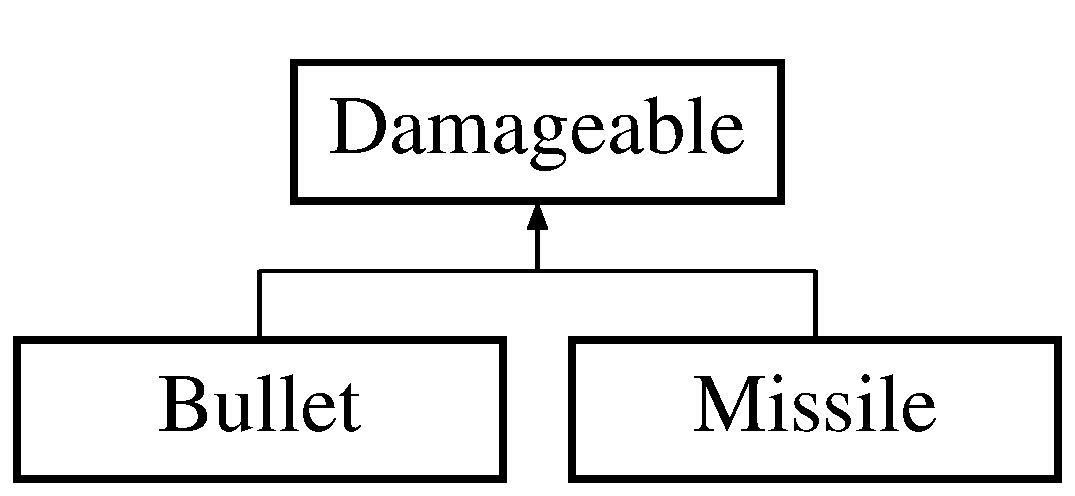
\includegraphics[height=2.000000cm]{class_damageable}
\end{center}
\end{figure}
\subsection*{Public Member Functions}
\begin{DoxyCompactItemize}
\item 
\hyperlink{class_damageable_a429f388154f540370a2b0940e6c91d3b}{Damageable} (float damage)
\item 
virtual \hyperlink{class_damageable_a22765a2d6d315def71ad07ef125b2885}{$\sim$\+Damageable} ()
\item 
float \hyperlink{class_damageable_acb416815e3384e6386665fa70e526bbb}{get\+Damage} ()
\end{DoxyCompactItemize}


\subsection{Constructor \& Destructor Documentation}
\hypertarget{class_damageable_a429f388154f540370a2b0940e6c91d3b}{}\label{class_damageable_a429f388154f540370a2b0940e6c91d3b} 
\index{Damageable@{Damageable}!Damageable@{Damageable}}
\index{Damageable@{Damageable}!Damageable@{Damageable}}
\subsubsection{\texorpdfstring{Damageable()}{Damageable()}}
{\footnotesize\ttfamily Damageable\+::\+Damageable (\begin{DoxyParamCaption}\item[{float}]{damage }\end{DoxyParamCaption})\hspace{0.3cm}{\ttfamily [inline]}}

\hypertarget{class_damageable_a22765a2d6d315def71ad07ef125b2885}{}\label{class_damageable_a22765a2d6d315def71ad07ef125b2885} 
\index{Damageable@{Damageable}!````~Damageable@{$\sim$\+Damageable}}
\index{````~Damageable@{$\sim$\+Damageable}!Damageable@{Damageable}}
\subsubsection{\texorpdfstring{$\sim$\+Damageable()}{~Damageable()}}
{\footnotesize\ttfamily virtual Damageable\+::$\sim$\+Damageable (\begin{DoxyParamCaption}{ }\end{DoxyParamCaption})\hspace{0.3cm}{\ttfamily [inline]}, {\ttfamily [virtual]}}



\subsection{Member Function Documentation}
\hypertarget{class_damageable_acb416815e3384e6386665fa70e526bbb}{}\label{class_damageable_acb416815e3384e6386665fa70e526bbb} 
\index{Damageable@{Damageable}!get\+Damage@{get\+Damage}}
\index{get\+Damage@{get\+Damage}!Damageable@{Damageable}}
\subsubsection{\texorpdfstring{get\+Damage()}{getDamage()}}
{\footnotesize\ttfamily float Damageable\+::get\+Damage (\begin{DoxyParamCaption}{ }\end{DoxyParamCaption})\hspace{0.3cm}{\ttfamily [inline]}}



The documentation for this class was generated from the following file\+:\begin{DoxyCompactItemize}
\item 
Console\+Application2/\hyperlink{_damage_object_8h}{Damage\+Object.\+h}\end{DoxyCompactItemize}

\hypertarget{class_entity_factory}{}\section{Entity\+Factory Class Reference}
\label{class_entity_factory}\index{Entity\+Factory@{Entity\+Factory}}


{\ttfamily \#include $<$Entity\+Factory.\+h$>$}

\subsection*{Static Public Member Functions}
\begin{DoxyCompactItemize}
\item 
static void \hyperlink{class_entity_factory_a09b1b21ae968b6db79f63824f9488091}{Create\+Missile} (\hyperlink{class_vector2_d}{Vector2D} position)
\item 
static void \hyperlink{class_entity_factory_a12afa2409278355f081201d888af9467}{Create\+Bullet} (\hyperlink{class_vector2_d}{Vector2D} position, \hyperlink{class_vector2_d}{Vector2D} direction, bool enemy\+Bullet=false)
\item 
static void \hyperlink{class_entity_factory_a9aa7edc76e6f6ee4158ae78b780f1e18}{Create\+Mutant} (\hyperlink{class_vector2_d}{Vector2D} position)
\item 
static void \hyperlink{class_entity_factory_a679ed3727e2f00e4fe15576c7fd5144d}{Create\+Meteor} ()
\item 
static void \hyperlink{class_entity_factory_a900ad8e29d0d8f27e6b4c981f25a7a58}{Create\+Abductor} (sf\+::\+Vector2f position)
\item 
static void \hyperlink{class_entity_factory_a855dd969520879d9ea167d854ca30c11}{Create\+Nest} (\hyperlink{class_vector2_d}{Vector2D} pos, \hyperlink{class_vector2_d}{Vector2D} dir, float speed)
\item 
static void \hyperlink{class_entity_factory_a825d95311fabc8edee88c6dda69346f4}{Create\+Astronaut} (float x\+Position)
\item 
static void \hyperlink{class_entity_factory_a3d50f46ea571447791681e0799fe7056}{Create\+Power\+Up} (int type, sf\+::\+Vector2f position)
\item 
static std\+::vector$<$ \hyperlink{class_game_object}{Game\+Object} $\ast$ $>$ \hyperlink{class_entity_factory_ab67a24301fabebc078f219c7e9e8c4fb}{get\+New\+Objects} ()
\item 
static std\+::vector$<$ \hyperlink{class_game_object}{Game\+Object} $\ast$ $>$ \hyperlink{class_entity_factory_a01479e6b22f3db318007b1dbc4e85058}{get\+New\+Objects\+Behind} ()
\item 
static void \hyperlink{class_entity_factory_a242fb009eda7ff8ff51025fd3d6a1e23}{clear\+Objects} ()
\item 
static void \hyperlink{class_entity_factory_ad55d3285456e3d8e03d27d274ac60d00}{abductor\+Death\+Notify} ()
\item 
static void \hyperlink{class_entity_factory_a7a2d1bf2e09b30ae6db3ee7f060763d8}{initialize} (sf\+::\+Float\+Rect level\+Size)
\end{DoxyCompactItemize}


\subsection{Member Function Documentation}
\hypertarget{class_entity_factory_ad55d3285456e3d8e03d27d274ac60d00}{}\label{class_entity_factory_ad55d3285456e3d8e03d27d274ac60d00} 
\index{Entity\+Factory@{Entity\+Factory}!abductor\+Death\+Notify@{abductor\+Death\+Notify}}
\index{abductor\+Death\+Notify@{abductor\+Death\+Notify}!Entity\+Factory@{Entity\+Factory}}
\subsubsection{\texorpdfstring{abductor\+Death\+Notify()}{abductorDeathNotify()}}
{\footnotesize\ttfamily void Entity\+Factory\+::abductor\+Death\+Notify (\begin{DoxyParamCaption}{ }\end{DoxyParamCaption})\hspace{0.3cm}{\ttfamily [static]}}

\hypertarget{class_entity_factory_a242fb009eda7ff8ff51025fd3d6a1e23}{}\label{class_entity_factory_a242fb009eda7ff8ff51025fd3d6a1e23} 
\index{Entity\+Factory@{Entity\+Factory}!clear\+Objects@{clear\+Objects}}
\index{clear\+Objects@{clear\+Objects}!Entity\+Factory@{Entity\+Factory}}
\subsubsection{\texorpdfstring{clear\+Objects()}{clearObjects()}}
{\footnotesize\ttfamily void Entity\+Factory\+::clear\+Objects (\begin{DoxyParamCaption}{ }\end{DoxyParamCaption})\hspace{0.3cm}{\ttfamily [static]}}

\hypertarget{class_entity_factory_a900ad8e29d0d8f27e6b4c981f25a7a58}{}\label{class_entity_factory_a900ad8e29d0d8f27e6b4c981f25a7a58} 
\index{Entity\+Factory@{Entity\+Factory}!Create\+Abductor@{Create\+Abductor}}
\index{Create\+Abductor@{Create\+Abductor}!Entity\+Factory@{Entity\+Factory}}
\subsubsection{\texorpdfstring{Create\+Abductor()}{CreateAbductor()}}
{\footnotesize\ttfamily void Entity\+Factory\+::\+Create\+Abductor (\begin{DoxyParamCaption}\item[{sf\+::\+Vector2f}]{position }\end{DoxyParamCaption})\hspace{0.3cm}{\ttfamily [static]}}

\hypertarget{class_entity_factory_a825d95311fabc8edee88c6dda69346f4}{}\label{class_entity_factory_a825d95311fabc8edee88c6dda69346f4} 
\index{Entity\+Factory@{Entity\+Factory}!Create\+Astronaut@{Create\+Astronaut}}
\index{Create\+Astronaut@{Create\+Astronaut}!Entity\+Factory@{Entity\+Factory}}
\subsubsection{\texorpdfstring{Create\+Astronaut()}{CreateAstronaut()}}
{\footnotesize\ttfamily void Entity\+Factory\+::\+Create\+Astronaut (\begin{DoxyParamCaption}\item[{float}]{x\+Position }\end{DoxyParamCaption})\hspace{0.3cm}{\ttfamily [static]}}

\hypertarget{class_entity_factory_a12afa2409278355f081201d888af9467}{}\label{class_entity_factory_a12afa2409278355f081201d888af9467} 
\index{Entity\+Factory@{Entity\+Factory}!Create\+Bullet@{Create\+Bullet}}
\index{Create\+Bullet@{Create\+Bullet}!Entity\+Factory@{Entity\+Factory}}
\subsubsection{\texorpdfstring{Create\+Bullet()}{CreateBullet()}}
{\footnotesize\ttfamily void Entity\+Factory\+::\+Create\+Bullet (\begin{DoxyParamCaption}\item[{\hyperlink{class_vector2_d}{Vector2D}}]{position,  }\item[{\hyperlink{class_vector2_d}{Vector2D}}]{direction,  }\item[{bool}]{enemy\+Bullet = {\ttfamily false} }\end{DoxyParamCaption})\hspace{0.3cm}{\ttfamily [static]}}

\hypertarget{class_entity_factory_a679ed3727e2f00e4fe15576c7fd5144d}{}\label{class_entity_factory_a679ed3727e2f00e4fe15576c7fd5144d} 
\index{Entity\+Factory@{Entity\+Factory}!Create\+Meteor@{Create\+Meteor}}
\index{Create\+Meteor@{Create\+Meteor}!Entity\+Factory@{Entity\+Factory}}
\subsubsection{\texorpdfstring{Create\+Meteor()}{CreateMeteor()}}
{\footnotesize\ttfamily void Entity\+Factory\+::\+Create\+Meteor (\begin{DoxyParamCaption}{ }\end{DoxyParamCaption})\hspace{0.3cm}{\ttfamily [static]}}

\hypertarget{class_entity_factory_a09b1b21ae968b6db79f63824f9488091}{}\label{class_entity_factory_a09b1b21ae968b6db79f63824f9488091} 
\index{Entity\+Factory@{Entity\+Factory}!Create\+Missile@{Create\+Missile}}
\index{Create\+Missile@{Create\+Missile}!Entity\+Factory@{Entity\+Factory}}
\subsubsection{\texorpdfstring{Create\+Missile()}{CreateMissile()}}
{\footnotesize\ttfamily void Entity\+Factory\+::\+Create\+Missile (\begin{DoxyParamCaption}\item[{\hyperlink{class_vector2_d}{Vector2D}}]{position }\end{DoxyParamCaption})\hspace{0.3cm}{\ttfamily [static]}}

\hypertarget{class_entity_factory_a9aa7edc76e6f6ee4158ae78b780f1e18}{}\label{class_entity_factory_a9aa7edc76e6f6ee4158ae78b780f1e18} 
\index{Entity\+Factory@{Entity\+Factory}!Create\+Mutant@{Create\+Mutant}}
\index{Create\+Mutant@{Create\+Mutant}!Entity\+Factory@{Entity\+Factory}}
\subsubsection{\texorpdfstring{Create\+Mutant()}{CreateMutant()}}
{\footnotesize\ttfamily void Entity\+Factory\+::\+Create\+Mutant (\begin{DoxyParamCaption}\item[{\hyperlink{class_vector2_d}{Vector2D}}]{position }\end{DoxyParamCaption})\hspace{0.3cm}{\ttfamily [static]}}

\hypertarget{class_entity_factory_a855dd969520879d9ea167d854ca30c11}{}\label{class_entity_factory_a855dd969520879d9ea167d854ca30c11} 
\index{Entity\+Factory@{Entity\+Factory}!Create\+Nest@{Create\+Nest}}
\index{Create\+Nest@{Create\+Nest}!Entity\+Factory@{Entity\+Factory}}
\subsubsection{\texorpdfstring{Create\+Nest()}{CreateNest()}}
{\footnotesize\ttfamily void Entity\+Factory\+::\+Create\+Nest (\begin{DoxyParamCaption}\item[{\hyperlink{class_vector2_d}{Vector2D}}]{pos,  }\item[{\hyperlink{class_vector2_d}{Vector2D}}]{dir,  }\item[{float}]{speed }\end{DoxyParamCaption})\hspace{0.3cm}{\ttfamily [static]}}

\hypertarget{class_entity_factory_a3d50f46ea571447791681e0799fe7056}{}\label{class_entity_factory_a3d50f46ea571447791681e0799fe7056} 
\index{Entity\+Factory@{Entity\+Factory}!Create\+Power\+Up@{Create\+Power\+Up}}
\index{Create\+Power\+Up@{Create\+Power\+Up}!Entity\+Factory@{Entity\+Factory}}
\subsubsection{\texorpdfstring{Create\+Power\+Up()}{CreatePowerUp()}}
{\footnotesize\ttfamily void Entity\+Factory\+::\+Create\+Power\+Up (\begin{DoxyParamCaption}\item[{int}]{type,  }\item[{sf\+::\+Vector2f}]{position }\end{DoxyParamCaption})\hspace{0.3cm}{\ttfamily [static]}}

\hypertarget{class_entity_factory_ab67a24301fabebc078f219c7e9e8c4fb}{}\label{class_entity_factory_ab67a24301fabebc078f219c7e9e8c4fb} 
\index{Entity\+Factory@{Entity\+Factory}!get\+New\+Objects@{get\+New\+Objects}}
\index{get\+New\+Objects@{get\+New\+Objects}!Entity\+Factory@{Entity\+Factory}}
\subsubsection{\texorpdfstring{get\+New\+Objects()}{getNewObjects()}}
{\footnotesize\ttfamily std\+::vector$<$ \hyperlink{class_game_object}{Game\+Object} $\ast$ $>$ Entity\+Factory\+::get\+New\+Objects (\begin{DoxyParamCaption}{ }\end{DoxyParamCaption})\hspace{0.3cm}{\ttfamily [static]}}

\hypertarget{class_entity_factory_a01479e6b22f3db318007b1dbc4e85058}{}\label{class_entity_factory_a01479e6b22f3db318007b1dbc4e85058} 
\index{Entity\+Factory@{Entity\+Factory}!get\+New\+Objects\+Behind@{get\+New\+Objects\+Behind}}
\index{get\+New\+Objects\+Behind@{get\+New\+Objects\+Behind}!Entity\+Factory@{Entity\+Factory}}
\subsubsection{\texorpdfstring{get\+New\+Objects\+Behind()}{getNewObjectsBehind()}}
{\footnotesize\ttfamily std\+::vector$<$ \hyperlink{class_game_object}{Game\+Object} $\ast$ $>$ Entity\+Factory\+::get\+New\+Objects\+Behind (\begin{DoxyParamCaption}{ }\end{DoxyParamCaption})\hspace{0.3cm}{\ttfamily [static]}}

\hypertarget{class_entity_factory_a7a2d1bf2e09b30ae6db3ee7f060763d8}{}\label{class_entity_factory_a7a2d1bf2e09b30ae6db3ee7f060763d8} 
\index{Entity\+Factory@{Entity\+Factory}!initialize@{initialize}}
\index{initialize@{initialize}!Entity\+Factory@{Entity\+Factory}}
\subsubsection{\texorpdfstring{initialize()}{initialize()}}
{\footnotesize\ttfamily void Entity\+Factory\+::initialize (\begin{DoxyParamCaption}\item[{sf\+::\+Float\+Rect}]{level\+Size }\end{DoxyParamCaption})\hspace{0.3cm}{\ttfamily [static]}}



The documentation for this class was generated from the following files\+:\begin{DoxyCompactItemize}
\item 
Console\+Application2/\hyperlink{_entity_factory_8h}{Entity\+Factory.\+h}\item 
Console\+Application2/\hyperlink{_entity_factory_8cpp}{Entity\+Factory.\+cpp}\end{DoxyCompactItemize}

\hypertarget{class_event_listener}{}\section{Event\+Listener Class Reference}
\label{class_event_listener}\index{Event\+Listener@{Event\+Listener}}


{\ttfamily \#include $<$Event\+Listener.\+h$>$}

Inheritance diagram for Event\+Listener\+:\begin{figure}[H]
\begin{center}
\leavevmode
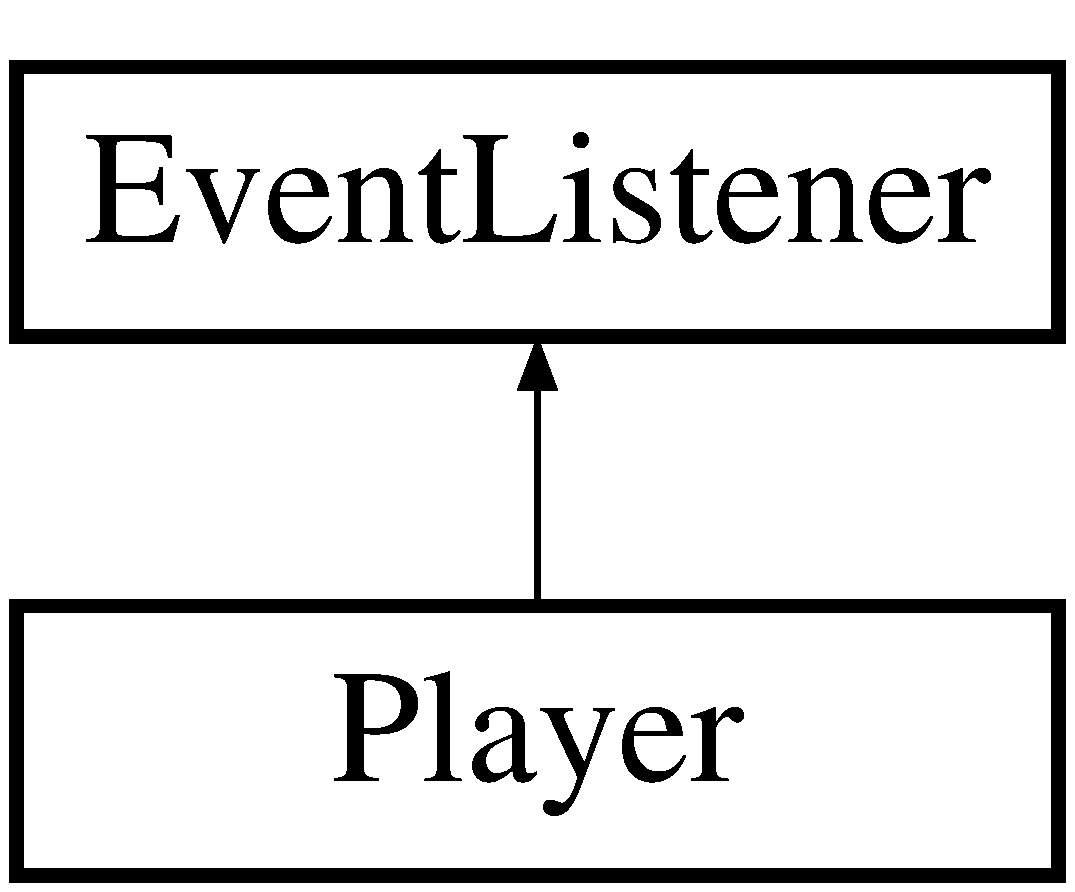
\includegraphics[height=2.000000cm]{class_event_listener}
\end{center}
\end{figure}
\subsection*{Public Types}
\begin{DoxyCompactItemize}
\item 
enum \hyperlink{class_event_listener_a23add62d02511a54eba0bae8208f9f48}{Generic\+Event} \{ \newline
\hyperlink{class_event_listener_a23add62d02511a54eba0bae8208f9f48a0504ea30baff7b670a10cb44f8e5cca2}{Generic\+Event\+::\+S\+H\+O\+OT}, 
\hyperlink{class_event_listener_a23add62d02511a54eba0bae8208f9f48ab405bd2177537a642d909c4313ce435c}{Generic\+Event\+::\+N\+O\+\_\+\+S\+H\+O\+OT}, 
\hyperlink{class_event_listener_a23add62d02511a54eba0bae8208f9f48ab539d21b829b50677302296d419f737f}{Generic\+Event\+::\+H\+Y\+P\+E\+R\+J\+U\+MP}, 
\hyperlink{class_event_listener_a23add62d02511a54eba0bae8208f9f48a608dc746696e8909ebb69d3bcabca44f}{Generic\+Event\+::\+S\+M\+A\+R\+T\+\_\+\+B\+O\+MB}, 
\newline
\hyperlink{class_event_listener_a23add62d02511a54eba0bae8208f9f48aefa0bff183da4bc574dc82011291f87a}{Generic\+Event\+::\+E\+MP}
 \}
\item 
enum \hyperlink{class_event_listener_ae72c5cb67f8dc880170bf2137837f6ce}{Key\+Down\+Event} \{ \hyperlink{class_event_listener_ae72c5cb67f8dc880170bf2137837f6ceafbaedde498cdead4f2780217646e9ba1}{Key\+Down\+Event\+::\+UP} = 10000, 
\hyperlink{class_event_listener_ae72c5cb67f8dc880170bf2137837f6cea684d325a7303f52e64011467ff5c5758}{Key\+Down\+Event\+::\+L\+E\+FT}, 
\hyperlink{class_event_listener_ae72c5cb67f8dc880170bf2137837f6ceac4e0e4e3118472beeb2ae75827450f1f}{Key\+Down\+Event\+::\+D\+O\+WN}, 
\hyperlink{class_event_listener_ae72c5cb67f8dc880170bf2137837f6cea21507b40c80068eda19865706fdc2403}{Key\+Down\+Event\+::\+R\+I\+G\+HT}
 \}
\item 
enum \hyperlink{class_event_listener_a69daf2aeedcab55e1f2c1c178206789e}{Key\+Up\+Event} \{ \hyperlink{class_event_listener_a69daf2aeedcab55e1f2c1c178206789eafbaedde498cdead4f2780217646e9ba1}{Key\+Up\+Event\+::\+UP} = 20000, 
\hyperlink{class_event_listener_a69daf2aeedcab55e1f2c1c178206789ea684d325a7303f52e64011467ff5c5758}{Key\+Up\+Event\+::\+L\+E\+FT}, 
\hyperlink{class_event_listener_a69daf2aeedcab55e1f2c1c178206789eac4e0e4e3118472beeb2ae75827450f1f}{Key\+Up\+Event\+::\+D\+O\+WN}, 
\hyperlink{class_event_listener_a69daf2aeedcab55e1f2c1c178206789ea21507b40c80068eda19865706fdc2403}{Key\+Up\+Event\+::\+R\+I\+G\+HT}
 \}
\end{DoxyCompactItemize}
\subsection*{Public Member Functions}
\begin{DoxyCompactItemize}
\item 
void \hyperlink{class_event_listener_a72427af914eb14753d02338556bfbda8}{on\+Event} (\hyperlink{class_event_listener_ae72c5cb67f8dc880170bf2137837f6ce}{Key\+Down\+Event} evt)
\item 
void \hyperlink{class_event_listener_a7f968abfca56b699a69b10a6c9af5902}{on\+Event} (\hyperlink{class_event_listener_a69daf2aeedcab55e1f2c1c178206789e}{Key\+Up\+Event} evt)
\item 
void \hyperlink{class_event_listener_aa29c811d59b30bf71e00a30d33c7f82c}{on\+Event} (\hyperlink{class_event_listener_a23add62d02511a54eba0bae8208f9f48}{Generic\+Event} evt)
\end{DoxyCompactItemize}


\subsection{Detailed Description}
Used as an interface for the event dispatcher 

\subsection{Member Enumeration Documentation}
\hypertarget{class_event_listener_a23add62d02511a54eba0bae8208f9f48}{}\label{class_event_listener_a23add62d02511a54eba0bae8208f9f48} 
\index{Event\+Listener@{Event\+Listener}!Generic\+Event@{Generic\+Event}}
\index{Generic\+Event@{Generic\+Event}!Event\+Listener@{Event\+Listener}}
\subsubsection{\texorpdfstring{Generic\+Event}{GenericEvent}}
{\footnotesize\ttfamily enum \hyperlink{class_event_listener_a23add62d02511a54eba0bae8208f9f48}{Event\+Listener\+::\+Generic\+Event}\hspace{0.3cm}{\ttfamily [strong]}}

\begin{DoxyEnumFields}{Enumerator}
\raisebox{\heightof{T}}[0pt][0pt]{\index{S\+H\+O\+OT@{S\+H\+O\+OT}!Event\+Listener@{Event\+Listener}}\index{Event\+Listener@{Event\+Listener}!S\+H\+O\+OT@{S\+H\+O\+OT}}}\hypertarget{class_event_listener_a23add62d02511a54eba0bae8208f9f48a0504ea30baff7b670a10cb44f8e5cca2}{}\label{class_event_listener_a23add62d02511a54eba0bae8208f9f48a0504ea30baff7b670a10cb44f8e5cca2} 
S\+H\+O\+OT&\\
\hline

\raisebox{\heightof{T}}[0pt][0pt]{\index{N\+O\+\_\+\+S\+H\+O\+OT@{N\+O\+\_\+\+S\+H\+O\+OT}!Event\+Listener@{Event\+Listener}}\index{Event\+Listener@{Event\+Listener}!N\+O\+\_\+\+S\+H\+O\+OT@{N\+O\+\_\+\+S\+H\+O\+OT}}}\hypertarget{class_event_listener_a23add62d02511a54eba0bae8208f9f48ab405bd2177537a642d909c4313ce435c}{}\label{class_event_listener_a23add62d02511a54eba0bae8208f9f48ab405bd2177537a642d909c4313ce435c} 
N\+O\+\_\+\+S\+H\+O\+OT&\\
\hline

\raisebox{\heightof{T}}[0pt][0pt]{\index{H\+Y\+P\+E\+R\+J\+U\+MP@{H\+Y\+P\+E\+R\+J\+U\+MP}!Event\+Listener@{Event\+Listener}}\index{Event\+Listener@{Event\+Listener}!H\+Y\+P\+E\+R\+J\+U\+MP@{H\+Y\+P\+E\+R\+J\+U\+MP}}}\hypertarget{class_event_listener_a23add62d02511a54eba0bae8208f9f48ab539d21b829b50677302296d419f737f}{}\label{class_event_listener_a23add62d02511a54eba0bae8208f9f48ab539d21b829b50677302296d419f737f} 
H\+Y\+P\+E\+R\+J\+U\+MP&\\
\hline

\raisebox{\heightof{T}}[0pt][0pt]{\index{S\+M\+A\+R\+T\+\_\+\+B\+O\+MB@{S\+M\+A\+R\+T\+\_\+\+B\+O\+MB}!Event\+Listener@{Event\+Listener}}\index{Event\+Listener@{Event\+Listener}!S\+M\+A\+R\+T\+\_\+\+B\+O\+MB@{S\+M\+A\+R\+T\+\_\+\+B\+O\+MB}}}\hypertarget{class_event_listener_a23add62d02511a54eba0bae8208f9f48a608dc746696e8909ebb69d3bcabca44f}{}\label{class_event_listener_a23add62d02511a54eba0bae8208f9f48a608dc746696e8909ebb69d3bcabca44f} 
S\+M\+A\+R\+T\+\_\+\+B\+O\+MB&\\
\hline

\raisebox{\heightof{T}}[0pt][0pt]{\index{E\+MP@{E\+MP}!Event\+Listener@{Event\+Listener}}\index{Event\+Listener@{Event\+Listener}!E\+MP@{E\+MP}}}\hypertarget{class_event_listener_a23add62d02511a54eba0bae8208f9f48aefa0bff183da4bc574dc82011291f87a}{}\label{class_event_listener_a23add62d02511a54eba0bae8208f9f48aefa0bff183da4bc574dc82011291f87a} 
E\+MP&\\
\hline

\end{DoxyEnumFields}
\hypertarget{class_event_listener_ae72c5cb67f8dc880170bf2137837f6ce}{}\label{class_event_listener_ae72c5cb67f8dc880170bf2137837f6ce} 
\index{Event\+Listener@{Event\+Listener}!Key\+Down\+Event@{Key\+Down\+Event}}
\index{Key\+Down\+Event@{Key\+Down\+Event}!Event\+Listener@{Event\+Listener}}
\subsubsection{\texorpdfstring{Key\+Down\+Event}{KeyDownEvent}}
{\footnotesize\ttfamily enum \hyperlink{class_event_listener_ae72c5cb67f8dc880170bf2137837f6ce}{Event\+Listener\+::\+Key\+Down\+Event}\hspace{0.3cm}{\ttfamily [strong]}}

\begin{DoxyEnumFields}{Enumerator}
\raisebox{\heightof{T}}[0pt][0pt]{\index{UP@{UP}!Event\+Listener@{Event\+Listener}}\index{Event\+Listener@{Event\+Listener}!UP@{UP}}}\hypertarget{class_event_listener_ae72c5cb67f8dc880170bf2137837f6ceafbaedde498cdead4f2780217646e9ba1}{}\label{class_event_listener_ae72c5cb67f8dc880170bf2137837f6ceafbaedde498cdead4f2780217646e9ba1} 
UP&\\
\hline

\raisebox{\heightof{T}}[0pt][0pt]{\index{L\+E\+FT@{L\+E\+FT}!Event\+Listener@{Event\+Listener}}\index{Event\+Listener@{Event\+Listener}!L\+E\+FT@{L\+E\+FT}}}\hypertarget{class_event_listener_ae72c5cb67f8dc880170bf2137837f6cea684d325a7303f52e64011467ff5c5758}{}\label{class_event_listener_ae72c5cb67f8dc880170bf2137837f6cea684d325a7303f52e64011467ff5c5758} 
L\+E\+FT&\\
\hline

\raisebox{\heightof{T}}[0pt][0pt]{\index{D\+O\+WN@{D\+O\+WN}!Event\+Listener@{Event\+Listener}}\index{Event\+Listener@{Event\+Listener}!D\+O\+WN@{D\+O\+WN}}}\hypertarget{class_event_listener_ae72c5cb67f8dc880170bf2137837f6ceac4e0e4e3118472beeb2ae75827450f1f}{}\label{class_event_listener_ae72c5cb67f8dc880170bf2137837f6ceac4e0e4e3118472beeb2ae75827450f1f} 
D\+O\+WN&\\
\hline

\raisebox{\heightof{T}}[0pt][0pt]{\index{R\+I\+G\+HT@{R\+I\+G\+HT}!Event\+Listener@{Event\+Listener}}\index{Event\+Listener@{Event\+Listener}!R\+I\+G\+HT@{R\+I\+G\+HT}}}\hypertarget{class_event_listener_ae72c5cb67f8dc880170bf2137837f6cea21507b40c80068eda19865706fdc2403}{}\label{class_event_listener_ae72c5cb67f8dc880170bf2137837f6cea21507b40c80068eda19865706fdc2403} 
R\+I\+G\+HT&\\
\hline

\end{DoxyEnumFields}
\hypertarget{class_event_listener_a69daf2aeedcab55e1f2c1c178206789e}{}\label{class_event_listener_a69daf2aeedcab55e1f2c1c178206789e} 
\index{Event\+Listener@{Event\+Listener}!Key\+Up\+Event@{Key\+Up\+Event}}
\index{Key\+Up\+Event@{Key\+Up\+Event}!Event\+Listener@{Event\+Listener}}
\subsubsection{\texorpdfstring{Key\+Up\+Event}{KeyUpEvent}}
{\footnotesize\ttfamily enum \hyperlink{class_event_listener_a69daf2aeedcab55e1f2c1c178206789e}{Event\+Listener\+::\+Key\+Up\+Event}\hspace{0.3cm}{\ttfamily [strong]}}

\begin{DoxyEnumFields}{Enumerator}
\raisebox{\heightof{T}}[0pt][0pt]{\index{UP@{UP}!Event\+Listener@{Event\+Listener}}\index{Event\+Listener@{Event\+Listener}!UP@{UP}}}\hypertarget{class_event_listener_a69daf2aeedcab55e1f2c1c178206789eafbaedde498cdead4f2780217646e9ba1}{}\label{class_event_listener_a69daf2aeedcab55e1f2c1c178206789eafbaedde498cdead4f2780217646e9ba1} 
UP&\\
\hline

\raisebox{\heightof{T}}[0pt][0pt]{\index{L\+E\+FT@{L\+E\+FT}!Event\+Listener@{Event\+Listener}}\index{Event\+Listener@{Event\+Listener}!L\+E\+FT@{L\+E\+FT}}}\hypertarget{class_event_listener_a69daf2aeedcab55e1f2c1c178206789ea684d325a7303f52e64011467ff5c5758}{}\label{class_event_listener_a69daf2aeedcab55e1f2c1c178206789ea684d325a7303f52e64011467ff5c5758} 
L\+E\+FT&\\
\hline

\raisebox{\heightof{T}}[0pt][0pt]{\index{D\+O\+WN@{D\+O\+WN}!Event\+Listener@{Event\+Listener}}\index{Event\+Listener@{Event\+Listener}!D\+O\+WN@{D\+O\+WN}}}\hypertarget{class_event_listener_a69daf2aeedcab55e1f2c1c178206789eac4e0e4e3118472beeb2ae75827450f1f}{}\label{class_event_listener_a69daf2aeedcab55e1f2c1c178206789eac4e0e4e3118472beeb2ae75827450f1f} 
D\+O\+WN&\\
\hline

\raisebox{\heightof{T}}[0pt][0pt]{\index{R\+I\+G\+HT@{R\+I\+G\+HT}!Event\+Listener@{Event\+Listener}}\index{Event\+Listener@{Event\+Listener}!R\+I\+G\+HT@{R\+I\+G\+HT}}}\hypertarget{class_event_listener_a69daf2aeedcab55e1f2c1c178206789ea21507b40c80068eda19865706fdc2403}{}\label{class_event_listener_a69daf2aeedcab55e1f2c1c178206789ea21507b40c80068eda19865706fdc2403} 
R\+I\+G\+HT&\\
\hline

\end{DoxyEnumFields}


\subsection{Member Function Documentation}
\hypertarget{class_event_listener_a72427af914eb14753d02338556bfbda8}{}\label{class_event_listener_a72427af914eb14753d02338556bfbda8} 
\index{Event\+Listener@{Event\+Listener}!on\+Event@{on\+Event}}
\index{on\+Event@{on\+Event}!Event\+Listener@{Event\+Listener}}
\subsubsection{\texorpdfstring{on\+Event()}{onEvent()}\hspace{0.1cm}{\footnotesize\ttfamily [1/3]}}
{\footnotesize\ttfamily void Event\+Listener\+::on\+Event (\begin{DoxyParamCaption}\item[{\hyperlink{class_event_listener_ae72c5cb67f8dc880170bf2137837f6ce}{Key\+Down\+Event}}]{evt }\end{DoxyParamCaption})\hspace{0.3cm}{\ttfamily [inline]}}

\hypertarget{class_event_listener_a7f968abfca56b699a69b10a6c9af5902}{}\label{class_event_listener_a7f968abfca56b699a69b10a6c9af5902} 
\index{Event\+Listener@{Event\+Listener}!on\+Event@{on\+Event}}
\index{on\+Event@{on\+Event}!Event\+Listener@{Event\+Listener}}
\subsubsection{\texorpdfstring{on\+Event()}{onEvent()}\hspace{0.1cm}{\footnotesize\ttfamily [2/3]}}
{\footnotesize\ttfamily void Event\+Listener\+::on\+Event (\begin{DoxyParamCaption}\item[{\hyperlink{class_event_listener_a69daf2aeedcab55e1f2c1c178206789e}{Key\+Up\+Event}}]{evt }\end{DoxyParamCaption})\hspace{0.3cm}{\ttfamily [inline]}}

\hypertarget{class_event_listener_aa29c811d59b30bf71e00a30d33c7f82c}{}\label{class_event_listener_aa29c811d59b30bf71e00a30d33c7f82c} 
\index{Event\+Listener@{Event\+Listener}!on\+Event@{on\+Event}}
\index{on\+Event@{on\+Event}!Event\+Listener@{Event\+Listener}}
\subsubsection{\texorpdfstring{on\+Event()}{onEvent()}\hspace{0.1cm}{\footnotesize\ttfamily [3/3]}}
{\footnotesize\ttfamily void Event\+Listener\+::on\+Event (\begin{DoxyParamCaption}\item[{\hyperlink{class_event_listener_a23add62d02511a54eba0bae8208f9f48}{Generic\+Event}}]{evt }\end{DoxyParamCaption})\hspace{0.3cm}{\ttfamily [inline]}}



The documentation for this class was generated from the following file\+:\begin{DoxyCompactItemize}
\item 
Console\+Application2/\hyperlink{_event_listener_8h}{Event\+Listener.\+h}\end{DoxyCompactItemize}

\hypertarget{class_game}{}\section{Game Class Reference}
\label{class_game}\index{Game@{Game}}


{\ttfamily \#include $<$Game.\+h$>$}

\subsection*{Public Member Functions}
\begin{DoxyCompactItemize}
\item 
\hyperlink{class_game_a9bf2dbc3669824fc9c0f86dbd5214ca8}{Game} (\hyperlink{class_vector2_d}{Vector2D} screen\+Size, \hyperlink{class_vector2_d}{Vector2D} level\+Size)
\item 
void \hyperlink{class_game_afa49214cd196fb9551341a84a8b45b4d}{Create\+Player} ()
\item 
void \hyperlink{class_game_a18399e8a53681f9cd22f969436ba151b}{Create\+Entities} (\hyperlink{class_vector2_d}{Vector2D} screen\+Size)
\item 
void \hyperlink{class_game_a4fa950db9b7e597d8b2595113a5629d2}{Update} (float dt)
\item 
void \hyperlink{class_game_af078573dbb338a48bfc485db6a92112d}{Update\+Game\+Object\+List} (float dt, std\+::vector$<$ \hyperlink{class_game_object}{Game\+Object} $\ast$$>$ \&list)
\item 
void \hyperlink{class_game_a5d49a201e628d0f6d5065260e8a429e1}{Add\+New\+Game\+Objects} ()
\item 
void \hyperlink{class_game_a43a5883ac1b2504aac1fdcffe8e8a897}{Draw} (sf\+::\+Render\+Window \&r)
\end{DoxyCompactItemize}


\subsection{Constructor \& Destructor Documentation}
\hypertarget{class_game_a9bf2dbc3669824fc9c0f86dbd5214ca8}{}\label{class_game_a9bf2dbc3669824fc9c0f86dbd5214ca8} 
\index{Game@{Game}!Game@{Game}}
\index{Game@{Game}!Game@{Game}}
\subsubsection{\texorpdfstring{Game()}{Game()}}
{\footnotesize\ttfamily Game\+::\+Game (\begin{DoxyParamCaption}\item[{\hyperlink{class_vector2_d}{Vector2D}}]{screen\+Size,  }\item[{\hyperlink{class_vector2_d}{Vector2D}}]{level\+Size }\end{DoxyParamCaption})}



\subsection{Member Function Documentation}
\hypertarget{class_game_a5d49a201e628d0f6d5065260e8a429e1}{}\label{class_game_a5d49a201e628d0f6d5065260e8a429e1} 
\index{Game@{Game}!Add\+New\+Game\+Objects@{Add\+New\+Game\+Objects}}
\index{Add\+New\+Game\+Objects@{Add\+New\+Game\+Objects}!Game@{Game}}
\subsubsection{\texorpdfstring{Add\+New\+Game\+Objects()}{AddNewGameObjects()}}
{\footnotesize\ttfamily void Game\+::\+Add\+New\+Game\+Objects (\begin{DoxyParamCaption}{ }\end{DoxyParamCaption})}

\hypertarget{class_game_a18399e8a53681f9cd22f969436ba151b}{}\label{class_game_a18399e8a53681f9cd22f969436ba151b} 
\index{Game@{Game}!Create\+Entities@{Create\+Entities}}
\index{Create\+Entities@{Create\+Entities}!Game@{Game}}
\subsubsection{\texorpdfstring{Create\+Entities()}{CreateEntities()}}
{\footnotesize\ttfamily void Game\+::\+Create\+Entities (\begin{DoxyParamCaption}\item[{\hyperlink{class_vector2_d}{Vector2D}}]{screen\+Size }\end{DoxyParamCaption})}

\hypertarget{class_game_afa49214cd196fb9551341a84a8b45b4d}{}\label{class_game_afa49214cd196fb9551341a84a8b45b4d} 
\index{Game@{Game}!Create\+Player@{Create\+Player}}
\index{Create\+Player@{Create\+Player}!Game@{Game}}
\subsubsection{\texorpdfstring{Create\+Player()}{CreatePlayer()}}
{\footnotesize\ttfamily void Game\+::\+Create\+Player (\begin{DoxyParamCaption}{ }\end{DoxyParamCaption})}

\hypertarget{class_game_a43a5883ac1b2504aac1fdcffe8e8a897}{}\label{class_game_a43a5883ac1b2504aac1fdcffe8e8a897} 
\index{Game@{Game}!Draw@{Draw}}
\index{Draw@{Draw}!Game@{Game}}
\subsubsection{\texorpdfstring{Draw()}{Draw()}}
{\footnotesize\ttfamily void Game\+::\+Draw (\begin{DoxyParamCaption}\item[{sf\+::\+Render\+Window \&}]{r }\end{DoxyParamCaption})}

\hypertarget{class_game_a4fa950db9b7e597d8b2595113a5629d2}{}\label{class_game_a4fa950db9b7e597d8b2595113a5629d2} 
\index{Game@{Game}!Update@{Update}}
\index{Update@{Update}!Game@{Game}}
\subsubsection{\texorpdfstring{Update()}{Update()}}
{\footnotesize\ttfamily void Game\+::\+Update (\begin{DoxyParamCaption}\item[{float}]{dt }\end{DoxyParamCaption})}

\hypertarget{class_game_af078573dbb338a48bfc485db6a92112d}{}\label{class_game_af078573dbb338a48bfc485db6a92112d} 
\index{Game@{Game}!Update\+Game\+Object\+List@{Update\+Game\+Object\+List}}
\index{Update\+Game\+Object\+List@{Update\+Game\+Object\+List}!Game@{Game}}
\subsubsection{\texorpdfstring{Update\+Game\+Object\+List()}{UpdateGameObjectList()}}
{\footnotesize\ttfamily void Game\+::\+Update\+Game\+Object\+List (\begin{DoxyParamCaption}\item[{float}]{dt,  }\item[{std\+::vector$<$ \hyperlink{class_game_object}{Game\+Object} $\ast$$>$ \&}]{list }\end{DoxyParamCaption})}



The documentation for this class was generated from the following files\+:\begin{DoxyCompactItemize}
\item 
Console\+Application2/\hyperlink{_game_8h}{Game.\+h}\item 
Console\+Application2/\hyperlink{_game_8cpp}{Game.\+cpp}\end{DoxyCompactItemize}

\hypertarget{class_game_object}{}\section{Game\+Object Class Reference}
\label{class_game_object}\index{Game\+Object@{Game\+Object}}


{\ttfamily \#include $<$Game\+Object.\+h$>$}

Inheritance diagram for Game\+Object\+:\begin{figure}[H]
\begin{center}
\leavevmode
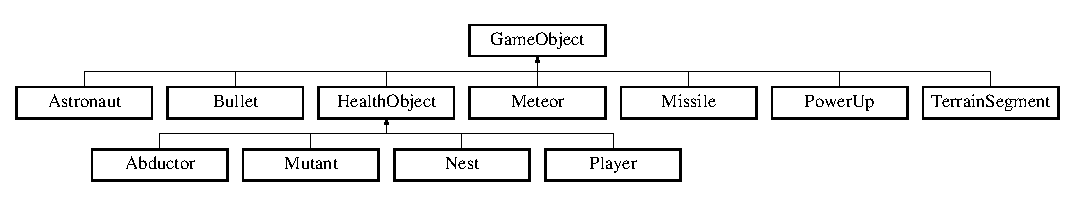
\includegraphics[height=2.201835cm]{class_game_object}
\end{center}
\end{figure}
\subsection*{Public Member Functions}
\begin{DoxyCompactItemize}
\item 
\hyperlink{class_game_object_aede2e0cfea6141c4fe0c8413e364d05a}{Game\+Object} (sf\+::\+Float\+Rect bounds, bool is\+Mini\+Map\+Object=false)
\item 
virtual \hyperlink{class_game_object_a224d4f6d9dd75c8a6f9d022eaf586fd9}{$\sim$\+Game\+Object} ()
\item 
virtual void \hyperlink{class_game_object_a93ed63df640deb516a020530e7f8e045}{Update} (float dt)=0
\item 
virtual void \hyperlink{class_game_object_a0bd45eb831b3d0959eb498cad3e412ce}{Draw} (sf\+::\+Render\+Window \&window)=0
\item 
virtual void \hyperlink{class_game_object_a8a3c07e92775fe00baa9e661fefb224e}{Draw\+With\+X\+Offset} (sf\+::\+Render\+Window \&window, float x\+Offset)=0
\item 
virtual bool \hyperlink{class_game_object_a86859eb19fa3f64529c83542ffa565e6}{Is\+Mini\+Map\+Object} ()
\item 
virtual sf\+::\+Float\+Rect \hyperlink{class_game_object_a4f5a473c0deffd85dc208d552cdb9018}{get\+A\+A\+BB} ()
\item 
virtual sf\+::\+Float\+Rect \hyperlink{class_game_object_a9d66c8590666d763d5fa0d380f534e3a}{get\+A\+A\+B\+B\+With\+X\+Offset} (float x\+Offset)
\item 
virtual void \hyperlink{class_game_object_adf9c98e9a2d3637bf57065d5a407e697}{set\+Bounds} (sf\+::\+Float\+Rect bounds)
\item 
virtual void \hyperlink{class_game_object_a53b129d55688652e25e6515d80e669ca}{wrap\+Positions} (\hyperlink{class_camera}{Camera} \&cam)
\item 
virtual void \hyperlink{class_game_object_a1c5da37ca4c3e7d2bfa8970eb9b5202d}{Damage} (float \+\_\+)
\item 
void \hyperlink{class_game_object_af54107b086de78b1fc6190088bdfb468}{kill} ()
\item 
bool \hyperlink{class_game_object_a2494b14b0e42549791b67d271503a0bc}{is\+Alive} ()
\end{DoxyCompactItemize}
\subsection*{Protected Attributes}
\begin{DoxyCompactItemize}
\item 
bool \hyperlink{class_game_object_a0ebb879c289d02bd83519e6c60dca27b}{m\+\_\+is\+Minimap\+Object}
\item 
sf\+::\+Float\+Rect \hyperlink{class_game_object_a6cb7e612660cf9ef98b573dd50407e20}{m\+\_\+bounds}
\end{DoxyCompactItemize}


\subsection{Constructor \& Destructor Documentation}
\hypertarget{class_game_object_aede2e0cfea6141c4fe0c8413e364d05a}{}\label{class_game_object_aede2e0cfea6141c4fe0c8413e364d05a} 
\index{Game\+Object@{Game\+Object}!Game\+Object@{Game\+Object}}
\index{Game\+Object@{Game\+Object}!Game\+Object@{Game\+Object}}
\subsubsection{\texorpdfstring{Game\+Object()}{GameObject()}}
{\footnotesize\ttfamily Game\+Object\+::\+Game\+Object (\begin{DoxyParamCaption}\item[{sf\+::\+Float\+Rect}]{bounds,  }\item[{bool}]{is\+Mini\+Map\+Object = {\ttfamily false} }\end{DoxyParamCaption})\hspace{0.3cm}{\ttfamily [inline]}}

\hypertarget{class_game_object_a224d4f6d9dd75c8a6f9d022eaf586fd9}{}\label{class_game_object_a224d4f6d9dd75c8a6f9d022eaf586fd9} 
\index{Game\+Object@{Game\+Object}!````~Game\+Object@{$\sim$\+Game\+Object}}
\index{````~Game\+Object@{$\sim$\+Game\+Object}!Game\+Object@{Game\+Object}}
\subsubsection{\texorpdfstring{$\sim$\+Game\+Object()}{~GameObject()}}
{\footnotesize\ttfamily virtual Game\+Object\+::$\sim$\+Game\+Object (\begin{DoxyParamCaption}{ }\end{DoxyParamCaption})\hspace{0.3cm}{\ttfamily [inline]}, {\ttfamily [virtual]}}



\subsection{Member Function Documentation}
\hypertarget{class_game_object_a1c5da37ca4c3e7d2bfa8970eb9b5202d}{}\label{class_game_object_a1c5da37ca4c3e7d2bfa8970eb9b5202d} 
\index{Game\+Object@{Game\+Object}!Damage@{Damage}}
\index{Damage@{Damage}!Game\+Object@{Game\+Object}}
\subsubsection{\texorpdfstring{Damage()}{Damage()}}
{\footnotesize\ttfamily virtual void Game\+Object\+::\+Damage (\begin{DoxyParamCaption}\item[{float}]{\+\_\+ }\end{DoxyParamCaption})\hspace{0.3cm}{\ttfamily [inline]}, {\ttfamily [virtual]}}



Reimplemented in \hyperlink{class_health_object_a782acdc8ee8f50ce7e4a7b76b2b474be}{Health\+Object}.

\hypertarget{class_game_object_a0bd45eb831b3d0959eb498cad3e412ce}{}\label{class_game_object_a0bd45eb831b3d0959eb498cad3e412ce} 
\index{Game\+Object@{Game\+Object}!Draw@{Draw}}
\index{Draw@{Draw}!Game\+Object@{Game\+Object}}
\subsubsection{\texorpdfstring{Draw()}{Draw()}}
{\footnotesize\ttfamily virtual void Game\+Object\+::\+Draw (\begin{DoxyParamCaption}\item[{sf\+::\+Render\+Window \&}]{window }\end{DoxyParamCaption})\hspace{0.3cm}{\ttfamily [pure virtual]}}



Implemented in \hyperlink{class_player_acc9dd8e10a4e219e7ac78a822a7cde7b}{Player}, \hyperlink{class_abductor_ab27e1580f1a11d483d97f028deda7370}{Abductor}, \hyperlink{class_astronaut_ad87f989c99c64de938c367865cd196c4}{Astronaut}, \hyperlink{class_bullet_a44b861616d73fd5cd0fe78af2acda9c1}{Bullet}, \hyperlink{class_power_up_a0f52fe4ae4e6e47fa3fd4fb2bcc2dcb7}{Power\+Up}, \hyperlink{class_missile_ae80d48e796f506e03e632122f62ae230}{Missile}, \hyperlink{class_mutant_a024a5caac9b29a79a4a505d36cfd3122}{Mutant}, \hyperlink{class_meteor_a426244847c2446f36016c4b06713ce10}{Meteor}, \hyperlink{class_nest_a5d38f9e047947336dd2830e936ce2386}{Nest}, and \hyperlink{class_terrain_segment_a288c66908f5eaf7974424f64a95d9a9a}{Terrain\+Segment}.

\hypertarget{class_game_object_a8a3c07e92775fe00baa9e661fefb224e}{}\label{class_game_object_a8a3c07e92775fe00baa9e661fefb224e} 
\index{Game\+Object@{Game\+Object}!Draw\+With\+X\+Offset@{Draw\+With\+X\+Offset}}
\index{Draw\+With\+X\+Offset@{Draw\+With\+X\+Offset}!Game\+Object@{Game\+Object}}
\subsubsection{\texorpdfstring{Draw\+With\+X\+Offset()}{DrawWithXOffset()}}
{\footnotesize\ttfamily virtual void Game\+Object\+::\+Draw\+With\+X\+Offset (\begin{DoxyParamCaption}\item[{sf\+::\+Render\+Window \&}]{window,  }\item[{float}]{x\+Offset }\end{DoxyParamCaption})\hspace{0.3cm}{\ttfamily [pure virtual]}}



Implemented in \hyperlink{class_player_ad977242aa8bda63737df338b5095a931}{Player}, \hyperlink{class_abductor_a6c68ecc2673674040f87c2409d8505a1}{Abductor}, \hyperlink{class_astronaut_ab37c4cce5348d86be1ec5ee652f5c917}{Astronaut}, \hyperlink{class_bullet_ae3696edcf0c726c8c1b18a62faef8c03}{Bullet}, \hyperlink{class_missile_a51c591552a2faedc78c524ea8ed3d770}{Missile}, \hyperlink{class_power_up_a4ddb447c9a6bdf1475bc2334590ba55e}{Power\+Up}, \hyperlink{class_mutant_a540fbecede166bd9c4ac68cbed72bc92}{Mutant}, \hyperlink{class_meteor_a6b3dc73ecbbf31c6869f7e79e0e266cc}{Meteor}, \hyperlink{class_nest_a43f88fdd7366b39bd7614f26433afe10}{Nest}, and \hyperlink{class_terrain_segment_ad9832f83e328b50f647bb844846fb095}{Terrain\+Segment}.

\hypertarget{class_game_object_a4f5a473c0deffd85dc208d552cdb9018}{}\label{class_game_object_a4f5a473c0deffd85dc208d552cdb9018} 
\index{Game\+Object@{Game\+Object}!get\+A\+A\+BB@{get\+A\+A\+BB}}
\index{get\+A\+A\+BB@{get\+A\+A\+BB}!Game\+Object@{Game\+Object}}
\subsubsection{\texorpdfstring{get\+A\+A\+B\+B()}{getAABB()}}
{\footnotesize\ttfamily virtual sf\+::\+Float\+Rect Game\+Object\+::get\+A\+A\+BB (\begin{DoxyParamCaption}{ }\end{DoxyParamCaption})\hspace{0.3cm}{\ttfamily [inline]}, {\ttfamily [virtual]}}

\hypertarget{class_game_object_a9d66c8590666d763d5fa0d380f534e3a}{}\label{class_game_object_a9d66c8590666d763d5fa0d380f534e3a} 
\index{Game\+Object@{Game\+Object}!get\+A\+A\+B\+B\+With\+X\+Offset@{get\+A\+A\+B\+B\+With\+X\+Offset}}
\index{get\+A\+A\+B\+B\+With\+X\+Offset@{get\+A\+A\+B\+B\+With\+X\+Offset}!Game\+Object@{Game\+Object}}
\subsubsection{\texorpdfstring{get\+A\+A\+B\+B\+With\+X\+Offset()}{getAABBWithXOffset()}}
{\footnotesize\ttfamily virtual sf\+::\+Float\+Rect Game\+Object\+::get\+A\+A\+B\+B\+With\+X\+Offset (\begin{DoxyParamCaption}\item[{float}]{x\+Offset }\end{DoxyParamCaption})\hspace{0.3cm}{\ttfamily [inline]}, {\ttfamily [virtual]}}

\hypertarget{class_game_object_a2494b14b0e42549791b67d271503a0bc}{}\label{class_game_object_a2494b14b0e42549791b67d271503a0bc} 
\index{Game\+Object@{Game\+Object}!is\+Alive@{is\+Alive}}
\index{is\+Alive@{is\+Alive}!Game\+Object@{Game\+Object}}
\subsubsection{\texorpdfstring{is\+Alive()}{isAlive()}}
{\footnotesize\ttfamily bool Game\+Object\+::is\+Alive (\begin{DoxyParamCaption}{ }\end{DoxyParamCaption})\hspace{0.3cm}{\ttfamily [inline]}}

\hypertarget{class_game_object_a86859eb19fa3f64529c83542ffa565e6}{}\label{class_game_object_a86859eb19fa3f64529c83542ffa565e6} 
\index{Game\+Object@{Game\+Object}!Is\+Mini\+Map\+Object@{Is\+Mini\+Map\+Object}}
\index{Is\+Mini\+Map\+Object@{Is\+Mini\+Map\+Object}!Game\+Object@{Game\+Object}}
\subsubsection{\texorpdfstring{Is\+Mini\+Map\+Object()}{IsMiniMapObject()}}
{\footnotesize\ttfamily virtual bool Game\+Object\+::\+Is\+Mini\+Map\+Object (\begin{DoxyParamCaption}{ }\end{DoxyParamCaption})\hspace{0.3cm}{\ttfamily [inline]}, {\ttfamily [virtual]}}

\hypertarget{class_game_object_af54107b086de78b1fc6190088bdfb468}{}\label{class_game_object_af54107b086de78b1fc6190088bdfb468} 
\index{Game\+Object@{Game\+Object}!kill@{kill}}
\index{kill@{kill}!Game\+Object@{Game\+Object}}
\subsubsection{\texorpdfstring{kill()}{kill()}}
{\footnotesize\ttfamily void Game\+Object\+::kill (\begin{DoxyParamCaption}{ }\end{DoxyParamCaption})\hspace{0.3cm}{\ttfamily [inline]}}

\hypertarget{class_game_object_adf9c98e9a2d3637bf57065d5a407e697}{}\label{class_game_object_adf9c98e9a2d3637bf57065d5a407e697} 
\index{Game\+Object@{Game\+Object}!set\+Bounds@{set\+Bounds}}
\index{set\+Bounds@{set\+Bounds}!Game\+Object@{Game\+Object}}
\subsubsection{\texorpdfstring{set\+Bounds()}{setBounds()}}
{\footnotesize\ttfamily virtual void Game\+Object\+::set\+Bounds (\begin{DoxyParamCaption}\item[{sf\+::\+Float\+Rect}]{bounds }\end{DoxyParamCaption})\hspace{0.3cm}{\ttfamily [inline]}, {\ttfamily [virtual]}}

\hypertarget{class_game_object_a93ed63df640deb516a020530e7f8e045}{}\label{class_game_object_a93ed63df640deb516a020530e7f8e045} 
\index{Game\+Object@{Game\+Object}!Update@{Update}}
\index{Update@{Update}!Game\+Object@{Game\+Object}}
\subsubsection{\texorpdfstring{Update()}{Update()}}
{\footnotesize\ttfamily virtual void Game\+Object\+::\+Update (\begin{DoxyParamCaption}\item[{float}]{dt }\end{DoxyParamCaption})\hspace{0.3cm}{\ttfamily [pure virtual]}}



Implemented in \hyperlink{class_player_a458939904cb2b2552089b841a5da5057}{Player}, \hyperlink{class_abductor_a16c030380d94caf386171cda40ed1eb8}{Abductor}, \hyperlink{class_astronaut_a808e903cd53b5ce1e18c781ec06b1ead}{Astronaut}, \hyperlink{class_bullet_a539b6ae5c3e6ae431f097296371e8d31}{Bullet}, \hyperlink{class_power_up_ab5d07a771930ebeadb6b8b0567436560}{Power\+Up}, \hyperlink{class_mutant_a69243115d28b18f3ac9803f66e8f8644}{Mutant}, \hyperlink{class_meteor_ab8f7e0d8ded9f7cf368db7841376fba6}{Meteor}, \hyperlink{class_nest_a00bd75873d812a893b20b0391ca117b4}{Nest}, \hyperlink{class_missile_a75c5c4613f289d4d0ad806743e7d40f7}{Missile}, and \hyperlink{class_terrain_segment_ac8a610b8011a973e775b0cf205ba473a}{Terrain\+Segment}.

\hypertarget{class_game_object_a53b129d55688652e25e6515d80e669ca}{}\label{class_game_object_a53b129d55688652e25e6515d80e669ca} 
\index{Game\+Object@{Game\+Object}!wrap\+Positions@{wrap\+Positions}}
\index{wrap\+Positions@{wrap\+Positions}!Game\+Object@{Game\+Object}}
\subsubsection{\texorpdfstring{wrap\+Positions()}{wrapPositions()}}
{\footnotesize\ttfamily void Game\+Object\+::wrap\+Positions (\begin{DoxyParamCaption}\item[{\hyperlink{class_camera}{Camera} \&}]{cam }\end{DoxyParamCaption})\hspace{0.3cm}{\ttfamily [virtual]}}



Reimplemented in \hyperlink{class_player_a09c333f62472d3ca96ef147126b518cd}{Player}, \hyperlink{class_abductor_a4623b394ad899b8df96b52e997fa5b03}{Abductor}, \hyperlink{class_astronaut_ab552db56a9d7341b3ce8f8a9b3670004}{Astronaut}, \hyperlink{class_bullet_ac33e38185d1800e4a532c71a620d1bf7}{Bullet}, \hyperlink{class_power_up_ad9ec62c1a3832e17949044c8349d0afb}{Power\+Up}, \hyperlink{class_mutant_a3bc5b923cb3605ddd10a5064ec904d29}{Mutant}, \hyperlink{class_meteor_a49fe47a23c6622f9850e81eac5c53ec2}{Meteor}, \hyperlink{class_nest_a763db342ea691c22d37b4905c1d022fa}{Nest}, and \hyperlink{class_missile_ae4d7aa6babf40ea774097bfa0f7c9ff7}{Missile}.



\subsection{Member Data Documentation}
\hypertarget{class_game_object_a6cb7e612660cf9ef98b573dd50407e20}{}\label{class_game_object_a6cb7e612660cf9ef98b573dd50407e20} 
\index{Game\+Object@{Game\+Object}!m\+\_\+bounds@{m\+\_\+bounds}}
\index{m\+\_\+bounds@{m\+\_\+bounds}!Game\+Object@{Game\+Object}}
\subsubsection{\texorpdfstring{m\+\_\+bounds}{m\_bounds}}
{\footnotesize\ttfamily sf\+::\+Float\+Rect Game\+Object\+::m\+\_\+bounds\hspace{0.3cm}{\ttfamily [protected]}}

\hypertarget{class_game_object_a0ebb879c289d02bd83519e6c60dca27b}{}\label{class_game_object_a0ebb879c289d02bd83519e6c60dca27b} 
\index{Game\+Object@{Game\+Object}!m\+\_\+is\+Minimap\+Object@{m\+\_\+is\+Minimap\+Object}}
\index{m\+\_\+is\+Minimap\+Object@{m\+\_\+is\+Minimap\+Object}!Game\+Object@{Game\+Object}}
\subsubsection{\texorpdfstring{m\+\_\+is\+Minimap\+Object}{m\_isMinimapObject}}
{\footnotesize\ttfamily bool Game\+Object\+::m\+\_\+is\+Minimap\+Object\hspace{0.3cm}{\ttfamily [protected]}}



The documentation for this class was generated from the following files\+:\begin{DoxyCompactItemize}
\item 
Console\+Application2/\hyperlink{_game_object_8h}{Game\+Object.\+h}\item 
Console\+Application2/\hyperlink{_game_object_8cpp}{Game\+Object.\+cpp}\end{DoxyCompactItemize}

\hypertarget{class_health_object}{}\section{Health\+Object Class Reference}
\label{class_health_object}\index{Health\+Object@{Health\+Object}}


{\ttfamily \#include $<$Health\+Object.\+h$>$}

Inheritance diagram for Health\+Object\+:\begin{figure}[H]
\begin{center}
\leavevmode
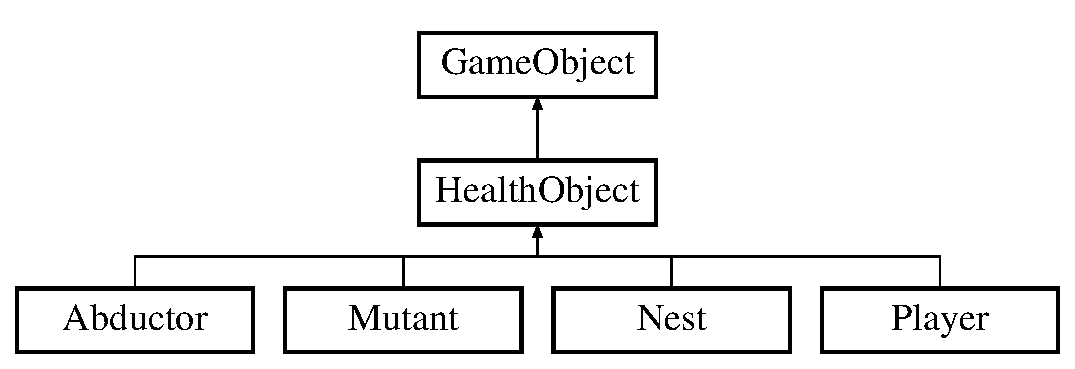
\includegraphics[height=3.000000cm]{class_health_object}
\end{center}
\end{figure}
\subsection*{Public Member Functions}
\begin{DoxyCompactItemize}
\item 
\hyperlink{class_health_object_af17b24dba0a4c4ff7c51b56124bad93a}{Health\+Object} (int max\+Health, sf\+::\+Float\+Rect bounds, bool is\+Minimap\+Object=false)
\item 
virtual \hyperlink{class_health_object_ac19c296f497bfca614d4742bafb4db9a}{$\sim$\+Health\+Object} ()
\item 
virtual void \hyperlink{class_health_object_a782acdc8ee8f50ce7e4a7b76b2b474be}{Damage} (float damage)
\end{DoxyCompactItemize}
\subsection*{Additional Inherited Members}


\subsection{Constructor \& Destructor Documentation}
\hypertarget{class_health_object_af17b24dba0a4c4ff7c51b56124bad93a}{}\label{class_health_object_af17b24dba0a4c4ff7c51b56124bad93a} 
\index{Health\+Object@{Health\+Object}!Health\+Object@{Health\+Object}}
\index{Health\+Object@{Health\+Object}!Health\+Object@{Health\+Object}}
\subsubsection{\texorpdfstring{Health\+Object()}{HealthObject()}}
{\footnotesize\ttfamily Health\+Object\+::\+Health\+Object (\begin{DoxyParamCaption}\item[{int}]{max\+Health,  }\item[{sf\+::\+Float\+Rect}]{bounds,  }\item[{bool}]{is\+Minimap\+Object = {\ttfamily false} }\end{DoxyParamCaption})}

\hypertarget{class_health_object_ac19c296f497bfca614d4742bafb4db9a}{}\label{class_health_object_ac19c296f497bfca614d4742bafb4db9a} 
\index{Health\+Object@{Health\+Object}!````~Health\+Object@{$\sim$\+Health\+Object}}
\index{````~Health\+Object@{$\sim$\+Health\+Object}!Health\+Object@{Health\+Object}}
\subsubsection{\texorpdfstring{$\sim$\+Health\+Object()}{~HealthObject()}}
{\footnotesize\ttfamily virtual Health\+Object\+::$\sim$\+Health\+Object (\begin{DoxyParamCaption}{ }\end{DoxyParamCaption})\hspace{0.3cm}{\ttfamily [inline]}, {\ttfamily [virtual]}}



\subsection{Member Function Documentation}
\hypertarget{class_health_object_a782acdc8ee8f50ce7e4a7b76b2b474be}{}\label{class_health_object_a782acdc8ee8f50ce7e4a7b76b2b474be} 
\index{Health\+Object@{Health\+Object}!Damage@{Damage}}
\index{Damage@{Damage}!Health\+Object@{Health\+Object}}
\subsubsection{\texorpdfstring{Damage()}{Damage()}}
{\footnotesize\ttfamily void Health\+Object\+::\+Damage (\begin{DoxyParamCaption}\item[{float}]{damage }\end{DoxyParamCaption})\hspace{0.3cm}{\ttfamily [virtual]}}



Reimplemented from \hyperlink{class_game_object_a1c5da37ca4c3e7d2bfa8970eb9b5202d}{Game\+Object}.



The documentation for this class was generated from the following files\+:\begin{DoxyCompactItemize}
\item 
Console\+Application2/\hyperlink{_health_object_8h}{Health\+Object.\+h}\item 
Console\+Application2/\hyperlink{_health_object_8cpp}{Health\+Object.\+cpp}\end{DoxyCompactItemize}

\hypertarget{class_input_manager}{}\section{Input\+Manager Class Reference}
\label{class_input_manager}\index{Input\+Manager@{Input\+Manager}}


{\ttfamily \#include $<$Input\+Manager.\+h$>$}

\subsection*{Public Member Functions}
\begin{DoxyCompactItemize}
\item 
\hyperlink{class_input_manager_af518290877dd183606709d5852db5491}{$\sim$\+Input\+Manager} ()
\item 
void \hyperlink{class_input_manager_a1f055ac31c702b3c4d183d9294b9aa6b}{Add\+Listener} (int, \hyperlink{class_event_listener}{Event\+Listener} $\ast$)
\item 
void \hyperlink{class_input_manager_a64666af03343a9065b8a0c7905aecd02}{Dispatch} (\hyperlink{class_event_listener_ae72c5cb67f8dc880170bf2137837f6ce}{Event\+Listener\+::\+Key\+Down\+Event})
\item 
void \hyperlink{class_input_manager_a9df2113b8d6c81099cebcbc80423a72e}{Dispatch} (\hyperlink{class_event_listener_a69daf2aeedcab55e1f2c1c178206789e}{Event\+Listener\+::\+Key\+Up\+Event})
\item 
void \hyperlink{class_input_manager_ac0c483ffc6437104b29f2e6f985f07ca}{Dispatch} (\hyperlink{class_event_listener_a23add62d02511a54eba0bae8208f9f48}{Event\+Listener\+::\+Generic\+Event})
\item 
void \hyperlink{class_input_manager_a0e4ced1e81e16392a445278e92d23ab9}{Process\+Input} (sf\+::\+Render\+Window $\ast$window)
\end{DoxyCompactItemize}
\subsection*{Static Public Member Functions}
\begin{DoxyCompactItemize}
\item 
static \hyperlink{class_input_manager}{Input\+Manager} $\ast$ \hyperlink{class_input_manager_a4d4852e7a0451fe53d9c116d8c3100d8}{get\+Instance} ()
\end{DoxyCompactItemize}


\subsection{Constructor \& Destructor Documentation}
\hypertarget{class_input_manager_af518290877dd183606709d5852db5491}{}\label{class_input_manager_af518290877dd183606709d5852db5491} 
\index{Input\+Manager@{Input\+Manager}!````~Input\+Manager@{$\sim$\+Input\+Manager}}
\index{````~Input\+Manager@{$\sim$\+Input\+Manager}!Input\+Manager@{Input\+Manager}}
\subsubsection{\texorpdfstring{$\sim$\+Input\+Manager()}{~InputManager()}}
{\footnotesize\ttfamily Input\+Manager\+::$\sim$\+Input\+Manager (\begin{DoxyParamCaption}{ }\end{DoxyParamCaption})}



\subsection{Member Function Documentation}
\hypertarget{class_input_manager_a1f055ac31c702b3c4d183d9294b9aa6b}{}\label{class_input_manager_a1f055ac31c702b3c4d183d9294b9aa6b} 
\index{Input\+Manager@{Input\+Manager}!Add\+Listener@{Add\+Listener}}
\index{Add\+Listener@{Add\+Listener}!Input\+Manager@{Input\+Manager}}
\subsubsection{\texorpdfstring{Add\+Listener()}{AddListener()}}
{\footnotesize\ttfamily void Input\+Manager\+::\+Add\+Listener (\begin{DoxyParamCaption}\item[{int}]{evt,  }\item[{\hyperlink{class_event_listener}{Event\+Listener} $\ast$}]{listener }\end{DoxyParamCaption})}

\hypertarget{class_input_manager_a64666af03343a9065b8a0c7905aecd02}{}\label{class_input_manager_a64666af03343a9065b8a0c7905aecd02} 
\index{Input\+Manager@{Input\+Manager}!Dispatch@{Dispatch}}
\index{Dispatch@{Dispatch}!Input\+Manager@{Input\+Manager}}
\subsubsection{\texorpdfstring{Dispatch()}{Dispatch()}\hspace{0.1cm}{\footnotesize\ttfamily [1/3]}}
{\footnotesize\ttfamily void Input\+Manager\+::\+Dispatch (\begin{DoxyParamCaption}\item[{\hyperlink{class_event_listener_ae72c5cb67f8dc880170bf2137837f6ce}{Event\+Listener\+::\+Key\+Down\+Event}}]{evt }\end{DoxyParamCaption})}

\hypertarget{class_input_manager_a9df2113b8d6c81099cebcbc80423a72e}{}\label{class_input_manager_a9df2113b8d6c81099cebcbc80423a72e} 
\index{Input\+Manager@{Input\+Manager}!Dispatch@{Dispatch}}
\index{Dispatch@{Dispatch}!Input\+Manager@{Input\+Manager}}
\subsubsection{\texorpdfstring{Dispatch()}{Dispatch()}\hspace{0.1cm}{\footnotesize\ttfamily [2/3]}}
{\footnotesize\ttfamily void Input\+Manager\+::\+Dispatch (\begin{DoxyParamCaption}\item[{\hyperlink{class_event_listener_a69daf2aeedcab55e1f2c1c178206789e}{Event\+Listener\+::\+Key\+Up\+Event}}]{evt }\end{DoxyParamCaption})}

\hypertarget{class_input_manager_ac0c483ffc6437104b29f2e6f985f07ca}{}\label{class_input_manager_ac0c483ffc6437104b29f2e6f985f07ca} 
\index{Input\+Manager@{Input\+Manager}!Dispatch@{Dispatch}}
\index{Dispatch@{Dispatch}!Input\+Manager@{Input\+Manager}}
\subsubsection{\texorpdfstring{Dispatch()}{Dispatch()}\hspace{0.1cm}{\footnotesize\ttfamily [3/3]}}
{\footnotesize\ttfamily void Input\+Manager\+::\+Dispatch (\begin{DoxyParamCaption}\item[{\hyperlink{class_event_listener_a23add62d02511a54eba0bae8208f9f48}{Event\+Listener\+::\+Generic\+Event}}]{evt }\end{DoxyParamCaption})}

\hypertarget{class_input_manager_a4d4852e7a0451fe53d9c116d8c3100d8}{}\label{class_input_manager_a4d4852e7a0451fe53d9c116d8c3100d8} 
\index{Input\+Manager@{Input\+Manager}!get\+Instance@{get\+Instance}}
\index{get\+Instance@{get\+Instance}!Input\+Manager@{Input\+Manager}}
\subsubsection{\texorpdfstring{get\+Instance()}{getInstance()}}
{\footnotesize\ttfamily \hyperlink{class_input_manager}{Input\+Manager} $\ast$ Input\+Manager\+::get\+Instance (\begin{DoxyParamCaption}{ }\end{DoxyParamCaption})\hspace{0.3cm}{\ttfamily [static]}}

\hypertarget{class_input_manager_a0e4ced1e81e16392a445278e92d23ab9}{}\label{class_input_manager_a0e4ced1e81e16392a445278e92d23ab9} 
\index{Input\+Manager@{Input\+Manager}!Process\+Input@{Process\+Input}}
\index{Process\+Input@{Process\+Input}!Input\+Manager@{Input\+Manager}}
\subsubsection{\texorpdfstring{Process\+Input()}{ProcessInput()}}
{\footnotesize\ttfamily void Input\+Manager\+::\+Process\+Input (\begin{DoxyParamCaption}\item[{sf\+::\+Render\+Window $\ast$}]{window }\end{DoxyParamCaption})}



The documentation for this class was generated from the following files\+:\begin{DoxyCompactItemize}
\item 
Console\+Application2/\hyperlink{_input_manager_8h}{Input\+Manager.\+h}\item 
Console\+Application2/\hyperlink{_input_manager_8cpp}{Input\+Manager.\+cpp}\end{DoxyCompactItemize}

\hypertarget{struct_load_exception}{}\section{Load\+Exception Struct Reference}
\label{struct_load_exception}\index{Load\+Exception@{Load\+Exception}}


{\ttfamily \#include $<$Asset\+Loader.\+h$>$}

Inheritance diagram for Load\+Exception\+:\begin{figure}[H]
\begin{center}
\leavevmode
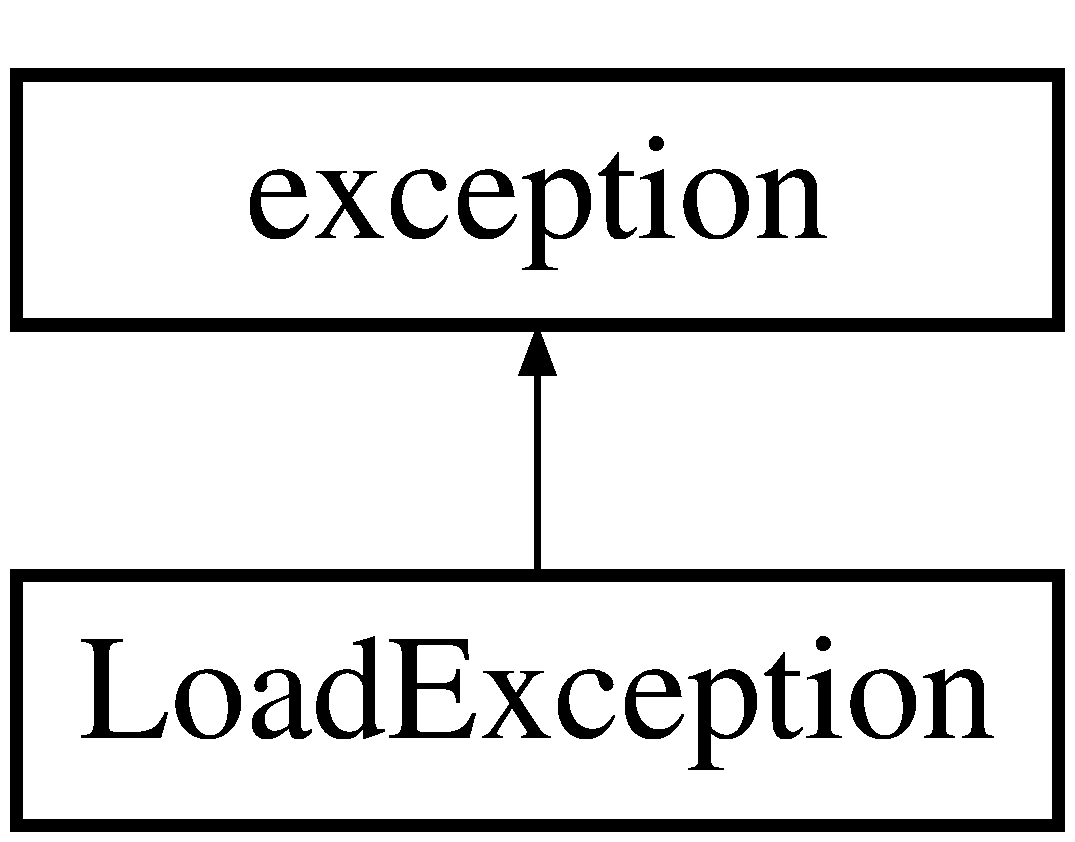
\includegraphics[height=2.000000cm]{struct_load_exception}
\end{center}
\end{figure}
\subsection*{Public Member Functions}
\begin{DoxyCompactItemize}
\item 
\hyperlink{struct_load_exception_a0dfeb76ded37d02c7765826842934f86}{Load\+Exception} (std\+::string ss)
\item 
\hyperlink{struct_load_exception_afb006cdbeb6ca9bab0c9bc3f7df9291b}{$\sim$\+Load\+Exception} ()  throw ()
\item 
const char $\ast$ \hyperlink{struct_load_exception_aa77af17720977ac8f651a4678ecf672c}{what} () const  throw ()
\end{DoxyCompactItemize}
\subsection*{Public Attributes}
\begin{DoxyCompactItemize}
\item 
std\+::string \hyperlink{struct_load_exception_ac148fff547e53eac53f36a2eb18f312a}{s}
\end{DoxyCompactItemize}


\subsection{Constructor \& Destructor Documentation}
\hypertarget{struct_load_exception_a0dfeb76ded37d02c7765826842934f86}{}\label{struct_load_exception_a0dfeb76ded37d02c7765826842934f86} 
\index{Load\+Exception@{Load\+Exception}!Load\+Exception@{Load\+Exception}}
\index{Load\+Exception@{Load\+Exception}!Load\+Exception@{Load\+Exception}}
\subsubsection{\texorpdfstring{Load\+Exception()}{LoadException()}}
{\footnotesize\ttfamily Load\+Exception\+::\+Load\+Exception (\begin{DoxyParamCaption}\item[{std\+::string}]{ss }\end{DoxyParamCaption})\hspace{0.3cm}{\ttfamily [inline]}}

\hypertarget{struct_load_exception_afb006cdbeb6ca9bab0c9bc3f7df9291b}{}\label{struct_load_exception_afb006cdbeb6ca9bab0c9bc3f7df9291b} 
\index{Load\+Exception@{Load\+Exception}!````~Load\+Exception@{$\sim$\+Load\+Exception}}
\index{````~Load\+Exception@{$\sim$\+Load\+Exception}!Load\+Exception@{Load\+Exception}}
\subsubsection{\texorpdfstring{$\sim$\+Load\+Exception()}{~LoadException()}}
{\footnotesize\ttfamily Load\+Exception\+::$\sim$\+Load\+Exception (\begin{DoxyParamCaption}{ }\end{DoxyParamCaption}) throw  ) \hspace{0.3cm}{\ttfamily [inline]}}



\subsection{Member Function Documentation}
\hypertarget{struct_load_exception_aa77af17720977ac8f651a4678ecf672c}{}\label{struct_load_exception_aa77af17720977ac8f651a4678ecf672c} 
\index{Load\+Exception@{Load\+Exception}!what@{what}}
\index{what@{what}!Load\+Exception@{Load\+Exception}}
\subsubsection{\texorpdfstring{what()}{what()}}
{\footnotesize\ttfamily const char$\ast$ Load\+Exception\+::what (\begin{DoxyParamCaption}{ }\end{DoxyParamCaption}) const throw  ) \hspace{0.3cm}{\ttfamily [inline]}}



\subsection{Member Data Documentation}
\hypertarget{struct_load_exception_ac148fff547e53eac53f36a2eb18f312a}{}\label{struct_load_exception_ac148fff547e53eac53f36a2eb18f312a} 
\index{Load\+Exception@{Load\+Exception}!s@{s}}
\index{s@{s}!Load\+Exception@{Load\+Exception}}
\subsubsection{\texorpdfstring{s}{s}}
{\footnotesize\ttfamily std\+::string Load\+Exception\+::s}



The documentation for this struct was generated from the following file\+:\begin{DoxyCompactItemize}
\item 
Console\+Application2/\hyperlink{_asset_loader_8h}{Asset\+Loader.\+h}\end{DoxyCompactItemize}

\hypertarget{class_meteor}{}\section{Meteor Class Reference}
\label{class_meteor}\index{Meteor@{Meteor}}


{\ttfamily \#include $<$Meteor.\+h$>$}

Inheritance diagram for Meteor\+:\begin{figure}[H]
\begin{center}
\leavevmode
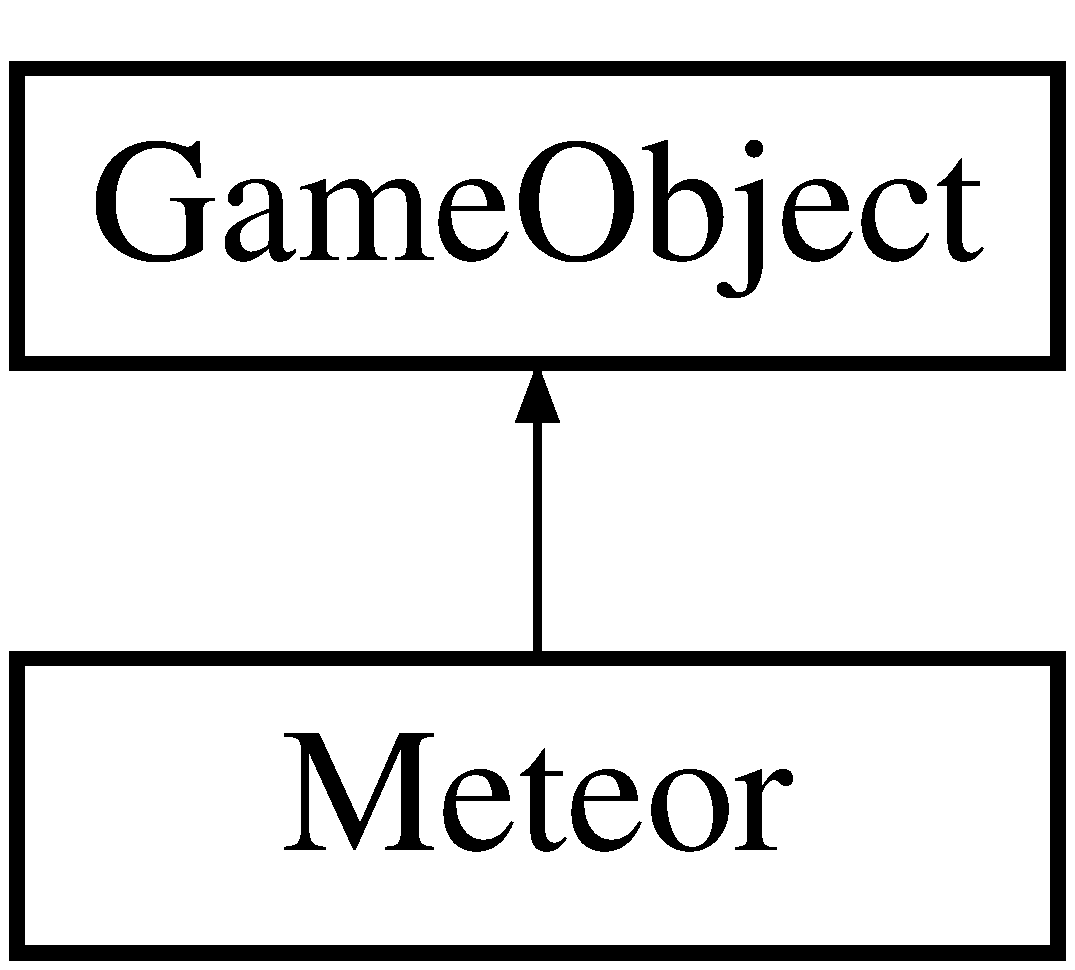
\includegraphics[height=2.000000cm]{class_meteor}
\end{center}
\end{figure}
\subsection*{Public Member Functions}
\begin{DoxyCompactItemize}
\item 
\hyperlink{class_meteor_ac3d2e6e2ed8395a62173117f283c0770}{Meteor} (\hyperlink{class_vector2_d}{Vector2D} position, float radius, float speed)
\item 
\hyperlink{class_meteor_aa4bfbce9a06fa010a5ef5213772efad8}{$\sim$\+Meteor} ()
\item 
void \hyperlink{class_meteor_ab8f7e0d8ded9f7cf368db7841376fba6}{Update} (float dt) override
\item 
void \hyperlink{class_meteor_a426244847c2446f36016c4b06713ce10}{Draw} (sf\+::\+Render\+Window \&w) override
\item 
void \hyperlink{class_meteor_a6b3dc73ecbbf31c6869f7e79e0e266cc}{Draw\+With\+X\+Offset} (sf\+::\+Render\+Window \&window, float x\+Offset) override
\item 
void \hyperlink{class_meteor_a49fe47a23c6622f9850e81eac5c53ec2}{wrap\+Positions} (\hyperlink{class_camera}{Camera} \&cam) override
\item 
\hyperlink{class_vector2_d}{Vector2D} \hyperlink{class_meteor_a28b006ae1f193fd0d0b3c2c19b82c278}{get\+Position} ()
\end{DoxyCompactItemize}
\subsection*{Additional Inherited Members}


\subsection{Constructor \& Destructor Documentation}
\hypertarget{class_meteor_ac3d2e6e2ed8395a62173117f283c0770}{}\label{class_meteor_ac3d2e6e2ed8395a62173117f283c0770} 
\index{Meteor@{Meteor}!Meteor@{Meteor}}
\index{Meteor@{Meteor}!Meteor@{Meteor}}
\subsubsection{\texorpdfstring{Meteor()}{Meteor()}}
{\footnotesize\ttfamily Meteor\+::\+Meteor (\begin{DoxyParamCaption}\item[{\hyperlink{class_vector2_d}{Vector2D}}]{position,  }\item[{float}]{radius,  }\item[{float}]{speed }\end{DoxyParamCaption})}

\hypertarget{class_meteor_aa4bfbce9a06fa010a5ef5213772efad8}{}\label{class_meteor_aa4bfbce9a06fa010a5ef5213772efad8} 
\index{Meteor@{Meteor}!````~Meteor@{$\sim$\+Meteor}}
\index{````~Meteor@{$\sim$\+Meteor}!Meteor@{Meteor}}
\subsubsection{\texorpdfstring{$\sim$\+Meteor()}{~Meteor()}}
{\footnotesize\ttfamily Meteor\+::$\sim$\+Meteor (\begin{DoxyParamCaption}{ }\end{DoxyParamCaption})}



\subsection{Member Function Documentation}
\hypertarget{class_meteor_a426244847c2446f36016c4b06713ce10}{}\label{class_meteor_a426244847c2446f36016c4b06713ce10} 
\index{Meteor@{Meteor}!Draw@{Draw}}
\index{Draw@{Draw}!Meteor@{Meteor}}
\subsubsection{\texorpdfstring{Draw()}{Draw()}}
{\footnotesize\ttfamily void Meteor\+::\+Draw (\begin{DoxyParamCaption}\item[{sf\+::\+Render\+Window \&}]{w }\end{DoxyParamCaption})\hspace{0.3cm}{\ttfamily [override]}, {\ttfamily [virtual]}}



Implements \hyperlink{class_game_object_a0bd45eb831b3d0959eb498cad3e412ce}{Game\+Object}.

\hypertarget{class_meteor_a6b3dc73ecbbf31c6869f7e79e0e266cc}{}\label{class_meteor_a6b3dc73ecbbf31c6869f7e79e0e266cc} 
\index{Meteor@{Meteor}!Draw\+With\+X\+Offset@{Draw\+With\+X\+Offset}}
\index{Draw\+With\+X\+Offset@{Draw\+With\+X\+Offset}!Meteor@{Meteor}}
\subsubsection{\texorpdfstring{Draw\+With\+X\+Offset()}{DrawWithXOffset()}}
{\footnotesize\ttfamily void Meteor\+::\+Draw\+With\+X\+Offset (\begin{DoxyParamCaption}\item[{sf\+::\+Render\+Window \&}]{window,  }\item[{float}]{x\+Offset }\end{DoxyParamCaption})\hspace{0.3cm}{\ttfamily [override]}, {\ttfamily [virtual]}}



Implements \hyperlink{class_game_object_a8a3c07e92775fe00baa9e661fefb224e}{Game\+Object}.

\hypertarget{class_meteor_a28b006ae1f193fd0d0b3c2c19b82c278}{}\label{class_meteor_a28b006ae1f193fd0d0b3c2c19b82c278} 
\index{Meteor@{Meteor}!get\+Position@{get\+Position}}
\index{get\+Position@{get\+Position}!Meteor@{Meteor}}
\subsubsection{\texorpdfstring{get\+Position()}{getPosition()}}
{\footnotesize\ttfamily \hyperlink{class_vector2_d}{Vector2D} Meteor\+::get\+Position (\begin{DoxyParamCaption}{ }\end{DoxyParamCaption})}

\hypertarget{class_meteor_ab8f7e0d8ded9f7cf368db7841376fba6}{}\label{class_meteor_ab8f7e0d8ded9f7cf368db7841376fba6} 
\index{Meteor@{Meteor}!Update@{Update}}
\index{Update@{Update}!Meteor@{Meteor}}
\subsubsection{\texorpdfstring{Update()}{Update()}}
{\footnotesize\ttfamily void Meteor\+::\+Update (\begin{DoxyParamCaption}\item[{float}]{dt }\end{DoxyParamCaption})\hspace{0.3cm}{\ttfamily [override]}, {\ttfamily [virtual]}}



Implements \hyperlink{class_game_object_a93ed63df640deb516a020530e7f8e045}{Game\+Object}.

\hypertarget{class_meteor_a49fe47a23c6622f9850e81eac5c53ec2}{}\label{class_meteor_a49fe47a23c6622f9850e81eac5c53ec2} 
\index{Meteor@{Meteor}!wrap\+Positions@{wrap\+Positions}}
\index{wrap\+Positions@{wrap\+Positions}!Meteor@{Meteor}}
\subsubsection{\texorpdfstring{wrap\+Positions()}{wrapPositions()}}
{\footnotesize\ttfamily void Meteor\+::wrap\+Positions (\begin{DoxyParamCaption}\item[{\hyperlink{class_camera}{Camera} \&}]{cam }\end{DoxyParamCaption})\hspace{0.3cm}{\ttfamily [override]}, {\ttfamily [virtual]}}



Reimplemented from \hyperlink{class_game_object_a53b129d55688652e25e6515d80e669ca}{Game\+Object}.



The documentation for this class was generated from the following files\+:\begin{DoxyCompactItemize}
\item 
Console\+Application2/\hyperlink{_meteor_8h}{Meteor.\+h}\item 
Console\+Application2/\hyperlink{_meteor_8cpp}{Meteor.\+cpp}\end{DoxyCompactItemize}

\hypertarget{class_missile}{}\section{Missile Class Reference}
\label{class_missile}\index{Missile@{Missile}}


{\ttfamily \#include $<$Missile.\+h$>$}

Inheritance diagram for Missile\+:\begin{figure}[H]
\begin{center}
\leavevmode
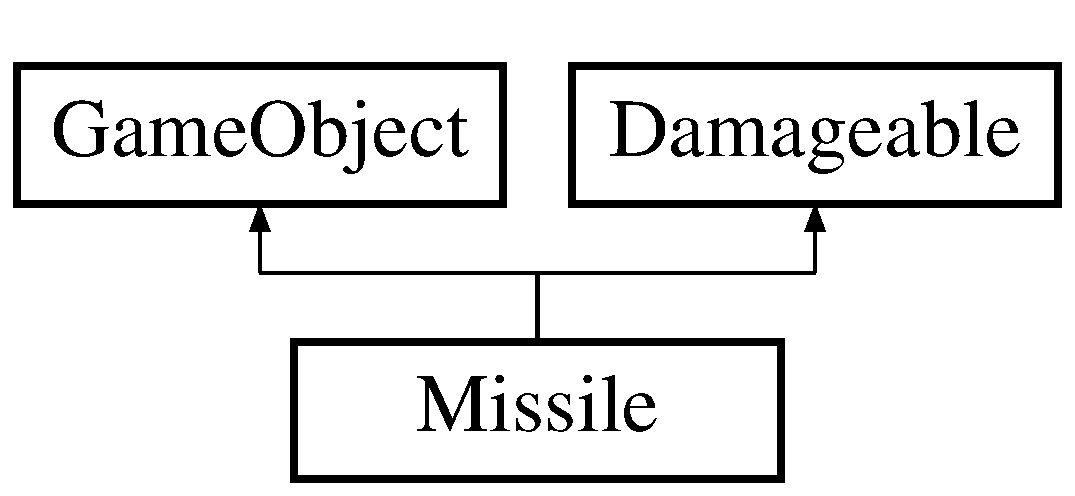
\includegraphics[height=2.000000cm]{class_missile}
\end{center}
\end{figure}
\subsection*{Public Member Functions}
\begin{DoxyCompactItemize}
\item 
\hyperlink{class_missile_acfe995db0f81c5bc53b6683d0081ab70}{Missile} (\hyperlink{class_vector2_d}{Vector2D} pos)
\item 
void \hyperlink{class_missile_a75c5c4613f289d4d0ad806743e7d40f7}{Update} (float dt) override
\item 
void \hyperlink{class_missile_ae4d7aa6babf40ea774097bfa0f7c9ff7}{wrap\+Positions} (\hyperlink{class_camera}{Camera} \&cam) override
\item 
void \hyperlink{class_missile_ae80d48e796f506e03e632122f62ae230}{Draw} (sf\+::\+Render\+Window \&w) override
\item 
void \hyperlink{class_missile_a51c591552a2faedc78c524ea8ed3d770}{Draw\+With\+X\+Offset} (sf\+::\+Render\+Window \&window, float x\+Offset) override
\end{DoxyCompactItemize}
\subsection*{Additional Inherited Members}


\subsection{Constructor \& Destructor Documentation}
\hypertarget{class_missile_acfe995db0f81c5bc53b6683d0081ab70}{}\label{class_missile_acfe995db0f81c5bc53b6683d0081ab70} 
\index{Missile@{Missile}!Missile@{Missile}}
\index{Missile@{Missile}!Missile@{Missile}}
\subsubsection{\texorpdfstring{Missile()}{Missile()}}
{\footnotesize\ttfamily Missile\+::\+Missile (\begin{DoxyParamCaption}\item[{\hyperlink{class_vector2_d}{Vector2D}}]{pos }\end{DoxyParamCaption})}



\subsection{Member Function Documentation}
\hypertarget{class_missile_ae80d48e796f506e03e632122f62ae230}{}\label{class_missile_ae80d48e796f506e03e632122f62ae230} 
\index{Missile@{Missile}!Draw@{Draw}}
\index{Draw@{Draw}!Missile@{Missile}}
\subsubsection{\texorpdfstring{Draw()}{Draw()}}
{\footnotesize\ttfamily void Missile\+::\+Draw (\begin{DoxyParamCaption}\item[{sf\+::\+Render\+Window \&}]{w }\end{DoxyParamCaption})\hspace{0.3cm}{\ttfamily [override]}, {\ttfamily [virtual]}}



Implements \hyperlink{class_game_object_a0bd45eb831b3d0959eb498cad3e412ce}{Game\+Object}.

\hypertarget{class_missile_a51c591552a2faedc78c524ea8ed3d770}{}\label{class_missile_a51c591552a2faedc78c524ea8ed3d770} 
\index{Missile@{Missile}!Draw\+With\+X\+Offset@{Draw\+With\+X\+Offset}}
\index{Draw\+With\+X\+Offset@{Draw\+With\+X\+Offset}!Missile@{Missile}}
\subsubsection{\texorpdfstring{Draw\+With\+X\+Offset()}{DrawWithXOffset()}}
{\footnotesize\ttfamily void Missile\+::\+Draw\+With\+X\+Offset (\begin{DoxyParamCaption}\item[{sf\+::\+Render\+Window \&}]{window,  }\item[{float}]{x\+Offset }\end{DoxyParamCaption})\hspace{0.3cm}{\ttfamily [override]}, {\ttfamily [virtual]}}



Implements \hyperlink{class_game_object_a8a3c07e92775fe00baa9e661fefb224e}{Game\+Object}.

\hypertarget{class_missile_a75c5c4613f289d4d0ad806743e7d40f7}{}\label{class_missile_a75c5c4613f289d4d0ad806743e7d40f7} 
\index{Missile@{Missile}!Update@{Update}}
\index{Update@{Update}!Missile@{Missile}}
\subsubsection{\texorpdfstring{Update()}{Update()}}
{\footnotesize\ttfamily void Missile\+::\+Update (\begin{DoxyParamCaption}\item[{float}]{dt }\end{DoxyParamCaption})\hspace{0.3cm}{\ttfamily [override]}, {\ttfamily [virtual]}}



Implements \hyperlink{class_game_object_a93ed63df640deb516a020530e7f8e045}{Game\+Object}.

\hypertarget{class_missile_ae4d7aa6babf40ea774097bfa0f7c9ff7}{}\label{class_missile_ae4d7aa6babf40ea774097bfa0f7c9ff7} 
\index{Missile@{Missile}!wrap\+Positions@{wrap\+Positions}}
\index{wrap\+Positions@{wrap\+Positions}!Missile@{Missile}}
\subsubsection{\texorpdfstring{wrap\+Positions()}{wrapPositions()}}
{\footnotesize\ttfamily void Missile\+::wrap\+Positions (\begin{DoxyParamCaption}\item[{\hyperlink{class_camera}{Camera} \&}]{cam }\end{DoxyParamCaption})\hspace{0.3cm}{\ttfamily [override]}, {\ttfamily [virtual]}}



Reimplemented from \hyperlink{class_game_object_a53b129d55688652e25e6515d80e669ca}{Game\+Object}.



The documentation for this class was generated from the following files\+:\begin{DoxyCompactItemize}
\item 
Console\+Application2/\hyperlink{_missile_8h}{Missile.\+h}\item 
Console\+Application2/\hyperlink{_missile_8cpp}{Missile.\+cpp}\end{DoxyCompactItemize}

\hypertarget{class_mutant}{}\section{Mutant Class Reference}
\label{class_mutant}\index{Mutant@{Mutant}}


{\ttfamily \#include $<$Mutant.\+h$>$}

Inheritance diagram for Mutant\+:\begin{figure}[H]
\begin{center}
\leavevmode
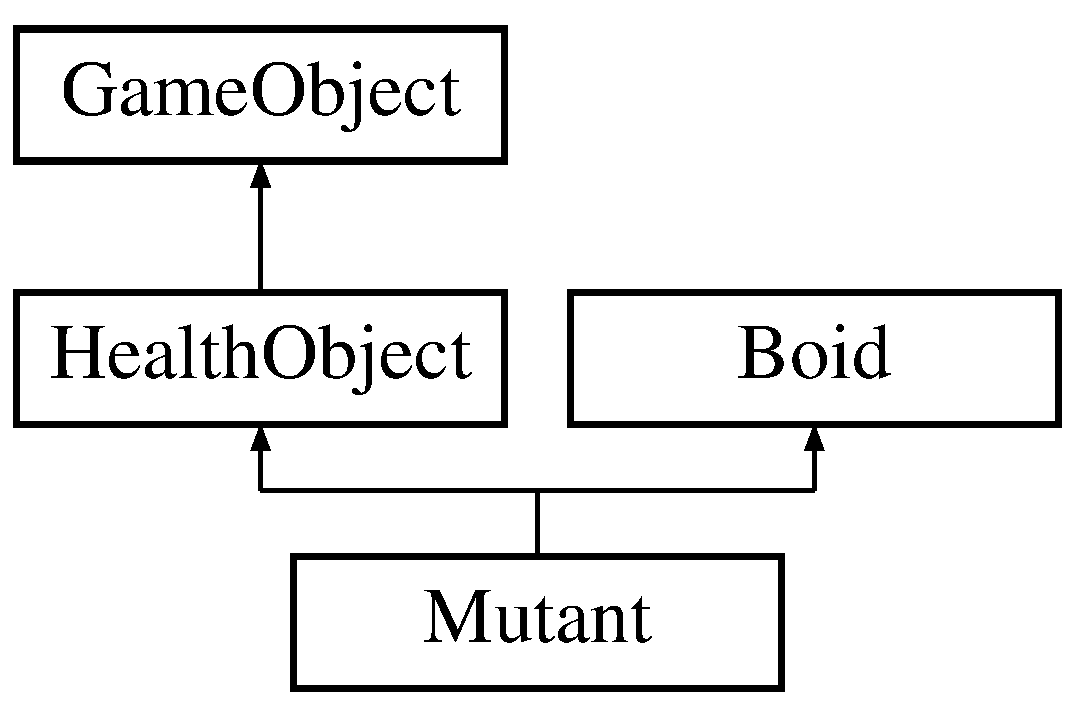
\includegraphics[height=3.000000cm]{class_mutant}
\end{center}
\end{figure}
\subsection*{Public Member Functions}
\begin{DoxyCompactItemize}
\item 
\hyperlink{class_mutant_aa054e45e945caaef4ca7777fa32190c2}{Mutant} (\hyperlink{class_vector2_d}{Vector2D} pos)
\item 
\hyperlink{class_vector2_d}{Vector2D} \hyperlink{class_mutant_a9c3ab53037fc85159e02643ecfe46717}{get\+Position} ()
\item 
\hyperlink{class_vector2_d}{Vector2D} \hyperlink{class_mutant_af26928fa19102fe5ebea774819c4c565}{get\+Velocity} ()
\item 
bool \hyperlink{class_mutant_a3416c1b42eb1e02bdcd4066109a28812}{is\+Predator} ()
\item 
void \hyperlink{class_mutant_a69243115d28b18f3ac9803f66e8f8644}{Update} (float dt)
\item 
void \hyperlink{class_mutant_a024a5caac9b29a79a4a505d36cfd3122}{Draw} (sf\+::\+Render\+Window \&window)
\item 
void \hyperlink{class_mutant_a540fbecede166bd9c4ac68cbed72bc92}{Draw\+With\+X\+Offset} (sf\+::\+Render\+Window \&window, float x\+Offset)
\item 
void \hyperlink{class_mutant_a3bc5b923cb3605ddd10a5064ec904d29}{wrap\+Positions} (\hyperlink{class_camera}{Camera} \&cam)
\item 
void \hyperlink{class_mutant_a5bbd6188efe9a18fa208bdaaf011ccdc}{destroy\+Electrics} ()
\item 
void \hyperlink{class_mutant_ac411f16b95e51f8e3c8c694425865785}{set\+GroundY} (float y)
\item 
bool \hyperlink{class_mutant_a67fc6ef40353436d04d847f49254fa0b}{is\+Under\+E\+MP} ()
\end{DoxyCompactItemize}
\subsection*{Additional Inherited Members}


\subsection{Constructor \& Destructor Documentation}
\hypertarget{class_mutant_aa054e45e945caaef4ca7777fa32190c2}{}\label{class_mutant_aa054e45e945caaef4ca7777fa32190c2} 
\index{Mutant@{Mutant}!Mutant@{Mutant}}
\index{Mutant@{Mutant}!Mutant@{Mutant}}
\subsubsection{\texorpdfstring{Mutant()}{Mutant()}}
{\footnotesize\ttfamily Mutant\+::\+Mutant (\begin{DoxyParamCaption}\item[{\hyperlink{class_vector2_d}{Vector2D}}]{pos }\end{DoxyParamCaption})}



\subsection{Member Function Documentation}
\hypertarget{class_mutant_a5bbd6188efe9a18fa208bdaaf011ccdc}{}\label{class_mutant_a5bbd6188efe9a18fa208bdaaf011ccdc} 
\index{Mutant@{Mutant}!destroy\+Electrics@{destroy\+Electrics}}
\index{destroy\+Electrics@{destroy\+Electrics}!Mutant@{Mutant}}
\subsubsection{\texorpdfstring{destroy\+Electrics()}{destroyElectrics()}}
{\footnotesize\ttfamily void Mutant\+::destroy\+Electrics (\begin{DoxyParamCaption}{ }\end{DoxyParamCaption})}

\hypertarget{class_mutant_a024a5caac9b29a79a4a505d36cfd3122}{}\label{class_mutant_a024a5caac9b29a79a4a505d36cfd3122} 
\index{Mutant@{Mutant}!Draw@{Draw}}
\index{Draw@{Draw}!Mutant@{Mutant}}
\subsubsection{\texorpdfstring{Draw()}{Draw()}}
{\footnotesize\ttfamily void Mutant\+::\+Draw (\begin{DoxyParamCaption}\item[{sf\+::\+Render\+Window \&}]{window }\end{DoxyParamCaption})\hspace{0.3cm}{\ttfamily [virtual]}}



Implements \hyperlink{class_game_object_a0bd45eb831b3d0959eb498cad3e412ce}{Game\+Object}.

\hypertarget{class_mutant_a540fbecede166bd9c4ac68cbed72bc92}{}\label{class_mutant_a540fbecede166bd9c4ac68cbed72bc92} 
\index{Mutant@{Mutant}!Draw\+With\+X\+Offset@{Draw\+With\+X\+Offset}}
\index{Draw\+With\+X\+Offset@{Draw\+With\+X\+Offset}!Mutant@{Mutant}}
\subsubsection{\texorpdfstring{Draw\+With\+X\+Offset()}{DrawWithXOffset()}}
{\footnotesize\ttfamily void Mutant\+::\+Draw\+With\+X\+Offset (\begin{DoxyParamCaption}\item[{sf\+::\+Render\+Window \&}]{window,  }\item[{float}]{x\+Offset }\end{DoxyParamCaption})\hspace{0.3cm}{\ttfamily [virtual]}}



Implements \hyperlink{class_game_object_a8a3c07e92775fe00baa9e661fefb224e}{Game\+Object}.

\hypertarget{class_mutant_a9c3ab53037fc85159e02643ecfe46717}{}\label{class_mutant_a9c3ab53037fc85159e02643ecfe46717} 
\index{Mutant@{Mutant}!get\+Position@{get\+Position}}
\index{get\+Position@{get\+Position}!Mutant@{Mutant}}
\subsubsection{\texorpdfstring{get\+Position()}{getPosition()}}
{\footnotesize\ttfamily \hyperlink{class_vector2_d}{Vector2D} Mutant\+::get\+Position (\begin{DoxyParamCaption}{ }\end{DoxyParamCaption})\hspace{0.3cm}{\ttfamily [virtual]}}



Implements \hyperlink{class_boid_a32f7601f73e7a109bbd79d43b15d2272}{Boid}.

\hypertarget{class_mutant_af26928fa19102fe5ebea774819c4c565}{}\label{class_mutant_af26928fa19102fe5ebea774819c4c565} 
\index{Mutant@{Mutant}!get\+Velocity@{get\+Velocity}}
\index{get\+Velocity@{get\+Velocity}!Mutant@{Mutant}}
\subsubsection{\texorpdfstring{get\+Velocity()}{getVelocity()}}
{\footnotesize\ttfamily \hyperlink{class_vector2_d}{Vector2D} Mutant\+::get\+Velocity (\begin{DoxyParamCaption}{ }\end{DoxyParamCaption})\hspace{0.3cm}{\ttfamily [virtual]}}



Implements \hyperlink{class_boid_a58472dead1db1399b75090bf48184619}{Boid}.

\hypertarget{class_mutant_a3416c1b42eb1e02bdcd4066109a28812}{}\label{class_mutant_a3416c1b42eb1e02bdcd4066109a28812} 
\index{Mutant@{Mutant}!is\+Predator@{is\+Predator}}
\index{is\+Predator@{is\+Predator}!Mutant@{Mutant}}
\subsubsection{\texorpdfstring{is\+Predator()}{isPredator()}}
{\footnotesize\ttfamily bool Mutant\+::is\+Predator (\begin{DoxyParamCaption}{ }\end{DoxyParamCaption})\hspace{0.3cm}{\ttfamily [virtual]}}



Implements \hyperlink{class_boid_afdc731ff7d6b7f471c202c191c4abf77}{Boid}.

\hypertarget{class_mutant_a67fc6ef40353436d04d847f49254fa0b}{}\label{class_mutant_a67fc6ef40353436d04d847f49254fa0b} 
\index{Mutant@{Mutant}!is\+Under\+E\+MP@{is\+Under\+E\+MP}}
\index{is\+Under\+E\+MP@{is\+Under\+E\+MP}!Mutant@{Mutant}}
\subsubsection{\texorpdfstring{is\+Under\+E\+M\+P()}{isUnderEMP()}}
{\footnotesize\ttfamily bool Mutant\+::is\+Under\+E\+MP (\begin{DoxyParamCaption}{ }\end{DoxyParamCaption})}

\hypertarget{class_mutant_ac411f16b95e51f8e3c8c694425865785}{}\label{class_mutant_ac411f16b95e51f8e3c8c694425865785} 
\index{Mutant@{Mutant}!set\+GroundY@{set\+GroundY}}
\index{set\+GroundY@{set\+GroundY}!Mutant@{Mutant}}
\subsubsection{\texorpdfstring{set\+Ground\+Y()}{setGroundY()}}
{\footnotesize\ttfamily void Mutant\+::set\+GroundY (\begin{DoxyParamCaption}\item[{float}]{y }\end{DoxyParamCaption})}

\hypertarget{class_mutant_a69243115d28b18f3ac9803f66e8f8644}{}\label{class_mutant_a69243115d28b18f3ac9803f66e8f8644} 
\index{Mutant@{Mutant}!Update@{Update}}
\index{Update@{Update}!Mutant@{Mutant}}
\subsubsection{\texorpdfstring{Update()}{Update()}}
{\footnotesize\ttfamily void Mutant\+::\+Update (\begin{DoxyParamCaption}\item[{float}]{dt }\end{DoxyParamCaption})\hspace{0.3cm}{\ttfamily [virtual]}}



Implements \hyperlink{class_game_object_a93ed63df640deb516a020530e7f8e045}{Game\+Object}.

\hypertarget{class_mutant_a3bc5b923cb3605ddd10a5064ec904d29}{}\label{class_mutant_a3bc5b923cb3605ddd10a5064ec904d29} 
\index{Mutant@{Mutant}!wrap\+Positions@{wrap\+Positions}}
\index{wrap\+Positions@{wrap\+Positions}!Mutant@{Mutant}}
\subsubsection{\texorpdfstring{wrap\+Positions()}{wrapPositions()}}
{\footnotesize\ttfamily void Mutant\+::wrap\+Positions (\begin{DoxyParamCaption}\item[{\hyperlink{class_camera}{Camera} \&}]{cam }\end{DoxyParamCaption})\hspace{0.3cm}{\ttfamily [virtual]}}



Reimplemented from \hyperlink{class_game_object_a53b129d55688652e25e6515d80e669ca}{Game\+Object}.



The documentation for this class was generated from the following files\+:\begin{DoxyCompactItemize}
\item 
Console\+Application2/\hyperlink{_mutant_8h}{Mutant.\+h}\item 
Console\+Application2/\hyperlink{_mutant_8cpp}{Mutant.\+cpp}\end{DoxyCompactItemize}

\hypertarget{class_nest}{}\section{Nest Class Reference}
\label{class_nest}\index{Nest@{Nest}}


{\ttfamily \#include $<$Nest.\+h$>$}

Inheritance diagram for Nest\+:\begin{figure}[H]
\begin{center}
\leavevmode
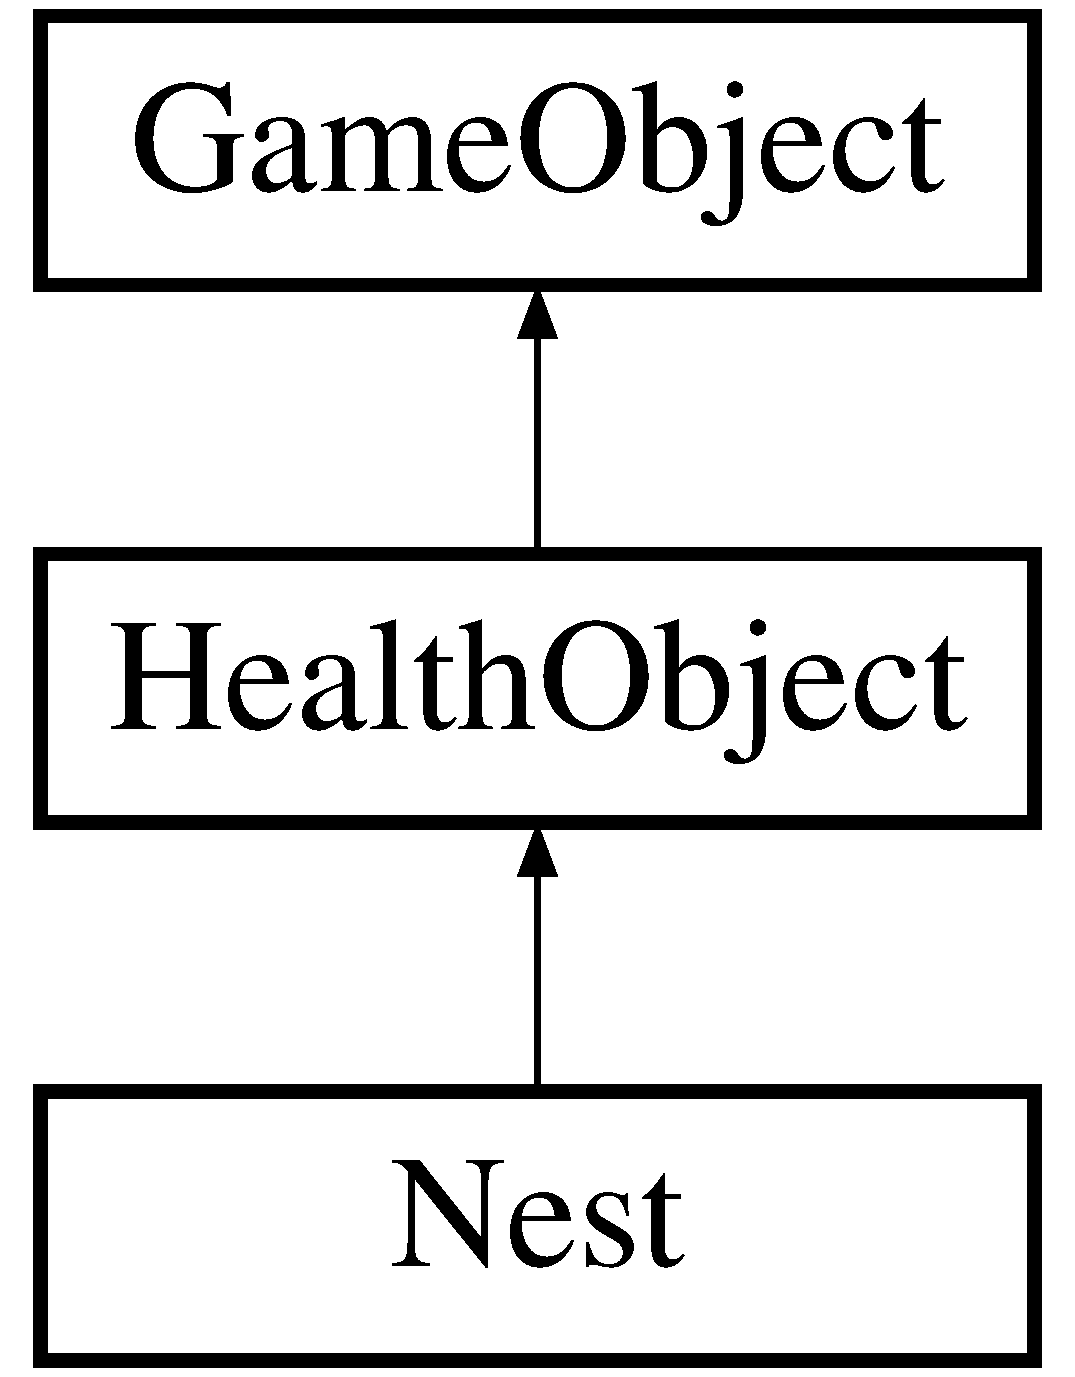
\includegraphics[height=3.000000cm]{class_nest}
\end{center}
\end{figure}
\subsection*{Public Member Functions}
\begin{DoxyCompactItemize}
\item 
\hyperlink{class_nest_a66b6012b3a0d2a9b00ec66cf5d312394}{Nest} (\hyperlink{class_vector2_d}{Vector2D} pos, \hyperlink{class_vector2_d}{Vector2D} dir, float speed)
\item 
void \hyperlink{class_nest_a5d38f9e047947336dd2830e936ce2386}{Draw} (sf\+::\+Render\+Window \&window) override
\item 
void \hyperlink{class_nest_a00bd75873d812a893b20b0391ca117b4}{Update} (float dt) override
\item 
void \hyperlink{class_nest_a43f88fdd7366b39bd7614f26433afe10}{Draw\+With\+X\+Offset} (sf\+::\+Render\+Window \&window, float x\+Offset) override
\item 
void \hyperlink{class_nest_a763db342ea691c22d37b4905c1d022fa}{wrap\+Positions} (\hyperlink{class_camera}{Camera} \&cam) override
\item 
void \hyperlink{class_nest_a981ac754a770ac168f034cb139b7726b}{Spawn\+Abductors} (float dt)
\item 
void \hyperlink{class_nest_a22039effa771e65a683e2dd084c04ded}{destroy\+Electrics} ()
\item 
void \hyperlink{class_nest_aa5a8307172777c880ba2747719a6a0f7}{set\+GroundY} (float y)
\item 
bool \hyperlink{class_nest_a436c3e1024545b8ce632105d2fac2c54}{is\+Under\+E\+MP} ()
\end{DoxyCompactItemize}
\subsection*{Additional Inherited Members}


\subsection{Constructor \& Destructor Documentation}
\hypertarget{class_nest_a66b6012b3a0d2a9b00ec66cf5d312394}{}\label{class_nest_a66b6012b3a0d2a9b00ec66cf5d312394} 
\index{Nest@{Nest}!Nest@{Nest}}
\index{Nest@{Nest}!Nest@{Nest}}
\subsubsection{\texorpdfstring{Nest()}{Nest()}}
{\footnotesize\ttfamily Nest\+::\+Nest (\begin{DoxyParamCaption}\item[{\hyperlink{class_vector2_d}{Vector2D}}]{pos,  }\item[{\hyperlink{class_vector2_d}{Vector2D}}]{dir,  }\item[{float}]{speed }\end{DoxyParamCaption})}



\subsection{Member Function Documentation}
\hypertarget{class_nest_a22039effa771e65a683e2dd084c04ded}{}\label{class_nest_a22039effa771e65a683e2dd084c04ded} 
\index{Nest@{Nest}!destroy\+Electrics@{destroy\+Electrics}}
\index{destroy\+Electrics@{destroy\+Electrics}!Nest@{Nest}}
\subsubsection{\texorpdfstring{destroy\+Electrics()}{destroyElectrics()}}
{\footnotesize\ttfamily void Nest\+::destroy\+Electrics (\begin{DoxyParamCaption}{ }\end{DoxyParamCaption})}

\hypertarget{class_nest_a5d38f9e047947336dd2830e936ce2386}{}\label{class_nest_a5d38f9e047947336dd2830e936ce2386} 
\index{Nest@{Nest}!Draw@{Draw}}
\index{Draw@{Draw}!Nest@{Nest}}
\subsubsection{\texorpdfstring{Draw()}{Draw()}}
{\footnotesize\ttfamily void Nest\+::\+Draw (\begin{DoxyParamCaption}\item[{sf\+::\+Render\+Window \&}]{window }\end{DoxyParamCaption})\hspace{0.3cm}{\ttfamily [override]}, {\ttfamily [virtual]}}



Implements \hyperlink{class_game_object_a0bd45eb831b3d0959eb498cad3e412ce}{Game\+Object}.

\hypertarget{class_nest_a43f88fdd7366b39bd7614f26433afe10}{}\label{class_nest_a43f88fdd7366b39bd7614f26433afe10} 
\index{Nest@{Nest}!Draw\+With\+X\+Offset@{Draw\+With\+X\+Offset}}
\index{Draw\+With\+X\+Offset@{Draw\+With\+X\+Offset}!Nest@{Nest}}
\subsubsection{\texorpdfstring{Draw\+With\+X\+Offset()}{DrawWithXOffset()}}
{\footnotesize\ttfamily void Nest\+::\+Draw\+With\+X\+Offset (\begin{DoxyParamCaption}\item[{sf\+::\+Render\+Window \&}]{window,  }\item[{float}]{x\+Offset }\end{DoxyParamCaption})\hspace{0.3cm}{\ttfamily [override]}, {\ttfamily [virtual]}}



Implements \hyperlink{class_game_object_a8a3c07e92775fe00baa9e661fefb224e}{Game\+Object}.

\hypertarget{class_nest_a436c3e1024545b8ce632105d2fac2c54}{}\label{class_nest_a436c3e1024545b8ce632105d2fac2c54} 
\index{Nest@{Nest}!is\+Under\+E\+MP@{is\+Under\+E\+MP}}
\index{is\+Under\+E\+MP@{is\+Under\+E\+MP}!Nest@{Nest}}
\subsubsection{\texorpdfstring{is\+Under\+E\+M\+P()}{isUnderEMP()}}
{\footnotesize\ttfamily bool Nest\+::is\+Under\+E\+MP (\begin{DoxyParamCaption}{ }\end{DoxyParamCaption})}

\hypertarget{class_nest_aa5a8307172777c880ba2747719a6a0f7}{}\label{class_nest_aa5a8307172777c880ba2747719a6a0f7} 
\index{Nest@{Nest}!set\+GroundY@{set\+GroundY}}
\index{set\+GroundY@{set\+GroundY}!Nest@{Nest}}
\subsubsection{\texorpdfstring{set\+Ground\+Y()}{setGroundY()}}
{\footnotesize\ttfamily void Nest\+::set\+GroundY (\begin{DoxyParamCaption}\item[{float}]{y }\end{DoxyParamCaption})}

\hypertarget{class_nest_a981ac754a770ac168f034cb139b7726b}{}\label{class_nest_a981ac754a770ac168f034cb139b7726b} 
\index{Nest@{Nest}!Spawn\+Abductors@{Spawn\+Abductors}}
\index{Spawn\+Abductors@{Spawn\+Abductors}!Nest@{Nest}}
\subsubsection{\texorpdfstring{Spawn\+Abductors()}{SpawnAbductors()}}
{\footnotesize\ttfamily void Nest\+::\+Spawn\+Abductors (\begin{DoxyParamCaption}\item[{float}]{dt }\end{DoxyParamCaption})}

\hypertarget{class_nest_a00bd75873d812a893b20b0391ca117b4}{}\label{class_nest_a00bd75873d812a893b20b0391ca117b4} 
\index{Nest@{Nest}!Update@{Update}}
\index{Update@{Update}!Nest@{Nest}}
\subsubsection{\texorpdfstring{Update()}{Update()}}
{\footnotesize\ttfamily void Nest\+::\+Update (\begin{DoxyParamCaption}\item[{float}]{dt }\end{DoxyParamCaption})\hspace{0.3cm}{\ttfamily [override]}, {\ttfamily [virtual]}}



Implements \hyperlink{class_game_object_a93ed63df640deb516a020530e7f8e045}{Game\+Object}.

\hypertarget{class_nest_a763db342ea691c22d37b4905c1d022fa}{}\label{class_nest_a763db342ea691c22d37b4905c1d022fa} 
\index{Nest@{Nest}!wrap\+Positions@{wrap\+Positions}}
\index{wrap\+Positions@{wrap\+Positions}!Nest@{Nest}}
\subsubsection{\texorpdfstring{wrap\+Positions()}{wrapPositions()}}
{\footnotesize\ttfamily void Nest\+::wrap\+Positions (\begin{DoxyParamCaption}\item[{\hyperlink{class_camera}{Camera} \&}]{cam }\end{DoxyParamCaption})\hspace{0.3cm}{\ttfamily [override]}, {\ttfamily [virtual]}}



Reimplemented from \hyperlink{class_game_object_a53b129d55688652e25e6515d80e669ca}{Game\+Object}.



The documentation for this class was generated from the following files\+:\begin{DoxyCompactItemize}
\item 
Console\+Application2/\hyperlink{_nest_8h}{Nest.\+h}\item 
Console\+Application2/\hyperlink{_nest_8cpp}{Nest.\+cpp}\end{DoxyCompactItemize}

\hypertarget{class_physics_manager}{}\section{Physics\+Manager Class Reference}
\label{class_physics_manager}\index{Physics\+Manager@{Physics\+Manager}}


{\ttfamily \#include $<$Physics\+Manager.\+h$>$}

\subsection*{Static Public Member Functions}
\begin{DoxyCompactItemize}
\item 
static void \hyperlink{class_physics_manager_afcc811e776c173c001762986adcfc731}{move} (float dt, \hyperlink{class_vector2_d}{Vector2D} \&position, \hyperlink{class_vector2_d}{Vector2D} \&velocity)
\item 
static void \hyperlink{class_physics_manager_ac91f12533b45cb7f7d66b82fbfd886fc}{accelerate} (float dt, \hyperlink{class_vector2_d}{Vector2D} \&speed, \hyperlink{class_vector2_d}{Vector2D} acceleration, \hyperlink{class_vector2_d}{Vector2D} target\+Speed)
\item 
static void \hyperlink{class_physics_manager_a74ec3035774192469d5e8560b80ddfd1}{accelerate\+Velocity} (float dt, \hyperlink{class_vector2_d}{Vector2D} \&velocity, \hyperlink{class_vector2_d}{Vector2D} acceleration, const float speed\+Limit)
\item 
static void \hyperlink{class_physics_manager_a75bfca00399793e604bcd749fa97c4ba}{Bind\+Position\+To\+Level} (\hyperlink{class_vector2_d}{Vector2D} \&m\+\_\+position, \hyperlink{class_vector2_d}{Vector2D} \&m\+\_\+direction)
\item 
static void \hyperlink{class_physics_manager_a8938f25d68d5e102f806ce7277814079}{Bind\+Position\+To\+Level} (\hyperlink{class_vector2_d}{Vector2D} \&m\+\_\+position)
\item 
static void \hyperlink{class_physics_manager_ad97cf48ec9c49605c4ca1be653cd0806}{Apply\+Friction} (float dt, \hyperlink{class_vector2_d}{Vector2D} \&velocity, float m\+Friction=0.\+01f)
\item 
static void \hyperlink{class_physics_manager_a754fec8e5f6ef692eb373d209689f897}{Vertical\+Wrap\+Position} (\hyperlink{class_vector2_d}{Vector2D} \&m\+\_\+position)
\item 
static void \hyperlink{class_physics_manager_aeae6dfda767bd621e02d44984ff7df8f}{initialize} (sf\+::\+Float\+Rect level\+Bounds)
\item 
static \hyperlink{class_vector2_d}{Vector2D} \hyperlink{class_physics_manager_a09f93d06f2a4a3855bedd13de9033fa5}{get\+Random\+Position} ()
\item 
static sf\+::\+Float\+Rect \hyperlink{class_physics_manager_ab6155905552f4740b0e5c9ee8a0de83f}{get\+Level\+Bounds} ()
\end{DoxyCompactItemize}


\subsection{Member Function Documentation}
\hypertarget{class_physics_manager_ac91f12533b45cb7f7d66b82fbfd886fc}{}\label{class_physics_manager_ac91f12533b45cb7f7d66b82fbfd886fc} 
\index{Physics\+Manager@{Physics\+Manager}!accelerate@{accelerate}}
\index{accelerate@{accelerate}!Physics\+Manager@{Physics\+Manager}}
\subsubsection{\texorpdfstring{accelerate()}{accelerate()}}
{\footnotesize\ttfamily void Physics\+Manager\+::accelerate (\begin{DoxyParamCaption}\item[{float}]{dt,  }\item[{\hyperlink{class_vector2_d}{Vector2D} \&}]{speed,  }\item[{\hyperlink{class_vector2_d}{Vector2D}}]{acceleration,  }\item[{\hyperlink{class_vector2_d}{Vector2D}}]{target\+Speed }\end{DoxyParamCaption})\hspace{0.3cm}{\ttfamily [static]}}

\hypertarget{class_physics_manager_a74ec3035774192469d5e8560b80ddfd1}{}\label{class_physics_manager_a74ec3035774192469d5e8560b80ddfd1} 
\index{Physics\+Manager@{Physics\+Manager}!accelerate\+Velocity@{accelerate\+Velocity}}
\index{accelerate\+Velocity@{accelerate\+Velocity}!Physics\+Manager@{Physics\+Manager}}
\subsubsection{\texorpdfstring{accelerate\+Velocity()}{accelerateVelocity()}}
{\footnotesize\ttfamily void Physics\+Manager\+::accelerate\+Velocity (\begin{DoxyParamCaption}\item[{float}]{dt,  }\item[{\hyperlink{class_vector2_d}{Vector2D} \&}]{velocity,  }\item[{\hyperlink{class_vector2_d}{Vector2D}}]{acceleration,  }\item[{const float}]{speed\+Limit }\end{DoxyParamCaption})\hspace{0.3cm}{\ttfamily [static]}}

\hypertarget{class_physics_manager_ad97cf48ec9c49605c4ca1be653cd0806}{}\label{class_physics_manager_ad97cf48ec9c49605c4ca1be653cd0806} 
\index{Physics\+Manager@{Physics\+Manager}!Apply\+Friction@{Apply\+Friction}}
\index{Apply\+Friction@{Apply\+Friction}!Physics\+Manager@{Physics\+Manager}}
\subsubsection{\texorpdfstring{Apply\+Friction()}{ApplyFriction()}}
{\footnotesize\ttfamily void Physics\+Manager\+::\+Apply\+Friction (\begin{DoxyParamCaption}\item[{float}]{dt,  }\item[{\hyperlink{class_vector2_d}{Vector2D} \&}]{velocity,  }\item[{float}]{m\+Friction = {\ttfamily 0.01f} }\end{DoxyParamCaption})\hspace{0.3cm}{\ttfamily [static]}}

\hypertarget{class_physics_manager_a75bfca00399793e604bcd749fa97c4ba}{}\label{class_physics_manager_a75bfca00399793e604bcd749fa97c4ba} 
\index{Physics\+Manager@{Physics\+Manager}!Bind\+Position\+To\+Level@{Bind\+Position\+To\+Level}}
\index{Bind\+Position\+To\+Level@{Bind\+Position\+To\+Level}!Physics\+Manager@{Physics\+Manager}}
\subsubsection{\texorpdfstring{Bind\+Position\+To\+Level()}{BindPositionToLevel()}\hspace{0.1cm}{\footnotesize\ttfamily [1/2]}}
{\footnotesize\ttfamily void Physics\+Manager\+::\+Bind\+Position\+To\+Level (\begin{DoxyParamCaption}\item[{\hyperlink{class_vector2_d}{Vector2D} \&}]{m\+\_\+position,  }\item[{\hyperlink{class_vector2_d}{Vector2D} \&}]{m\+\_\+direction }\end{DoxyParamCaption})\hspace{0.3cm}{\ttfamily [static]}}

\hypertarget{class_physics_manager_a8938f25d68d5e102f806ce7277814079}{}\label{class_physics_manager_a8938f25d68d5e102f806ce7277814079} 
\index{Physics\+Manager@{Physics\+Manager}!Bind\+Position\+To\+Level@{Bind\+Position\+To\+Level}}
\index{Bind\+Position\+To\+Level@{Bind\+Position\+To\+Level}!Physics\+Manager@{Physics\+Manager}}
\subsubsection{\texorpdfstring{Bind\+Position\+To\+Level()}{BindPositionToLevel()}\hspace{0.1cm}{\footnotesize\ttfamily [2/2]}}
{\footnotesize\ttfamily void Physics\+Manager\+::\+Bind\+Position\+To\+Level (\begin{DoxyParamCaption}\item[{\hyperlink{class_vector2_d}{Vector2D} \&}]{m\+\_\+position }\end{DoxyParamCaption})\hspace{0.3cm}{\ttfamily [static]}}

\hypertarget{class_physics_manager_ab6155905552f4740b0e5c9ee8a0de83f}{}\label{class_physics_manager_ab6155905552f4740b0e5c9ee8a0de83f} 
\index{Physics\+Manager@{Physics\+Manager}!get\+Level\+Bounds@{get\+Level\+Bounds}}
\index{get\+Level\+Bounds@{get\+Level\+Bounds}!Physics\+Manager@{Physics\+Manager}}
\subsubsection{\texorpdfstring{get\+Level\+Bounds()}{getLevelBounds()}}
{\footnotesize\ttfamily sf\+::\+Float\+Rect Physics\+Manager\+::get\+Level\+Bounds (\begin{DoxyParamCaption}{ }\end{DoxyParamCaption})\hspace{0.3cm}{\ttfamily [static]}}

\hypertarget{class_physics_manager_a09f93d06f2a4a3855bedd13de9033fa5}{}\label{class_physics_manager_a09f93d06f2a4a3855bedd13de9033fa5} 
\index{Physics\+Manager@{Physics\+Manager}!get\+Random\+Position@{get\+Random\+Position}}
\index{get\+Random\+Position@{get\+Random\+Position}!Physics\+Manager@{Physics\+Manager}}
\subsubsection{\texorpdfstring{get\+Random\+Position()}{getRandomPosition()}}
{\footnotesize\ttfamily \hyperlink{class_vector2_d}{Vector2D} Physics\+Manager\+::get\+Random\+Position (\begin{DoxyParamCaption}{ }\end{DoxyParamCaption})\hspace{0.3cm}{\ttfamily [static]}}

\hypertarget{class_physics_manager_aeae6dfda767bd621e02d44984ff7df8f}{}\label{class_physics_manager_aeae6dfda767bd621e02d44984ff7df8f} 
\index{Physics\+Manager@{Physics\+Manager}!initialize@{initialize}}
\index{initialize@{initialize}!Physics\+Manager@{Physics\+Manager}}
\subsubsection{\texorpdfstring{initialize()}{initialize()}}
{\footnotesize\ttfamily void Physics\+Manager\+::initialize (\begin{DoxyParamCaption}\item[{sf\+::\+Float\+Rect}]{level\+Bounds }\end{DoxyParamCaption})\hspace{0.3cm}{\ttfamily [static]}}

\hypertarget{class_physics_manager_afcc811e776c173c001762986adcfc731}{}\label{class_physics_manager_afcc811e776c173c001762986adcfc731} 
\index{Physics\+Manager@{Physics\+Manager}!move@{move}}
\index{move@{move}!Physics\+Manager@{Physics\+Manager}}
\subsubsection{\texorpdfstring{move()}{move()}}
{\footnotesize\ttfamily void Physics\+Manager\+::move (\begin{DoxyParamCaption}\item[{float}]{dt,  }\item[{\hyperlink{class_vector2_d}{Vector2D} \&}]{position,  }\item[{\hyperlink{class_vector2_d}{Vector2D} \&}]{velocity }\end{DoxyParamCaption})\hspace{0.3cm}{\ttfamily [static]}}

\hypertarget{class_physics_manager_a754fec8e5f6ef692eb373d209689f897}{}\label{class_physics_manager_a754fec8e5f6ef692eb373d209689f897} 
\index{Physics\+Manager@{Physics\+Manager}!Vertical\+Wrap\+Position@{Vertical\+Wrap\+Position}}
\index{Vertical\+Wrap\+Position@{Vertical\+Wrap\+Position}!Physics\+Manager@{Physics\+Manager}}
\subsubsection{\texorpdfstring{Vertical\+Wrap\+Position()}{VerticalWrapPosition()}}
{\footnotesize\ttfamily void Physics\+Manager\+::\+Vertical\+Wrap\+Position (\begin{DoxyParamCaption}\item[{\hyperlink{class_vector2_d}{Vector2D} \&}]{m\+\_\+position }\end{DoxyParamCaption})\hspace{0.3cm}{\ttfamily [static]}}



The documentation for this class was generated from the following files\+:\begin{DoxyCompactItemize}
\item 
Console\+Application2/\hyperlink{_physics_manager_8h}{Physics\+Manager.\+h}\item 
Console\+Application2/\hyperlink{_physics_manager_8cpp}{Physics\+Manager.\+cpp}\end{DoxyCompactItemize}

\hypertarget{class_player}{}\section{Player Class Reference}
\label{class_player}\index{Player@{Player}}


{\ttfamily \#include $<$Player.\+h$>$}

Inheritance diagram for Player\+:\begin{figure}[H]
\begin{center}
\leavevmode
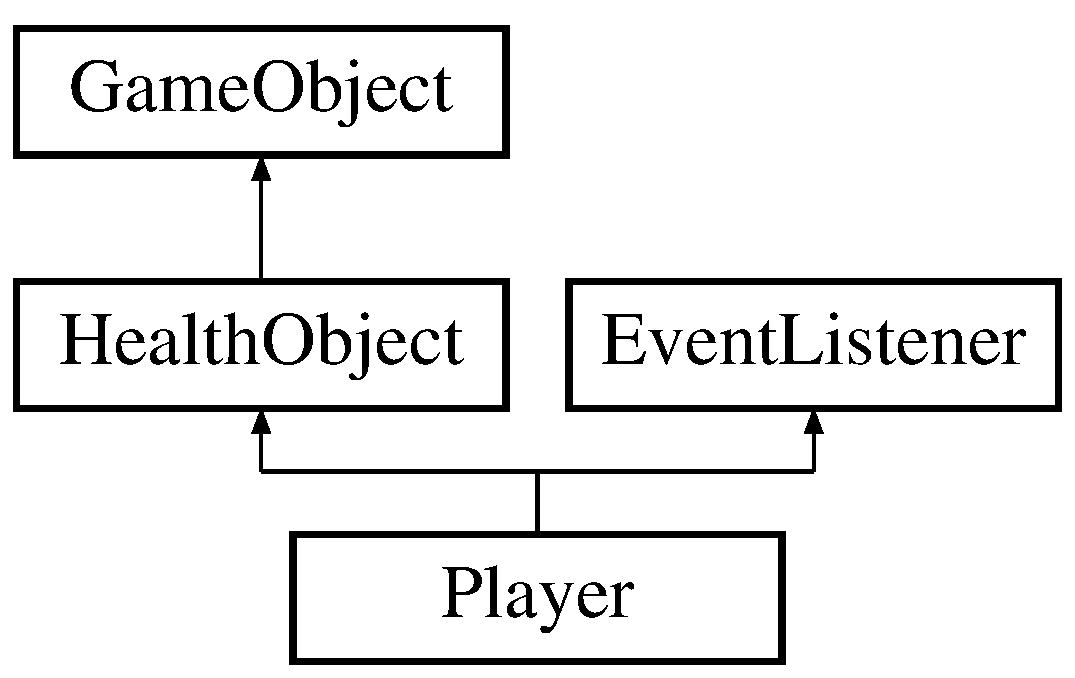
\includegraphics[height=3.000000cm]{class_player}
\end{center}
\end{figure}
\subsection*{Public Member Functions}
\begin{DoxyCompactItemize}
\item 
\hyperlink{class_player_a92008587897cd5b46c85e7d4df5f3b79}{Player} (sf\+::\+Vector2f position, sf\+::\+Vector2f size, \hyperlink{class_vector2_d}{Vector2D} acceleration, \hyperlink{class_vector2_d}{Vector2D} max\+Speed)
\item 
\hyperlink{class_player_a749d2c00e1fe0f5c2746f7505a58c062}{$\sim$\+Player} ()
\item 
void \hyperlink{class_player_a5685ccedbb647c6dc475581af3454851}{Initialize\+Events} ()
\item 
void \hyperlink{class_player_a458939904cb2b2552089b841a5da5057}{Update} (float dt) override
\item 
void \hyperlink{class_player_acc9dd8e10a4e219e7ac78a822a7cde7b}{Draw} (sf\+::\+Render\+Window \&w) override
\item 
void \hyperlink{class_player_ad977242aa8bda63737df338b5095a931}{Draw\+With\+X\+Offset} (sf\+::\+Render\+Window \&window, float x\+Offset) override
\item 
void \hyperlink{class_player_a450eb63d50f2127f4417f50fa926ca30}{on\+Generic\+Event} (\hyperlink{class_event_listener_a23add62d02511a54eba0bae8208f9f48}{Generic\+Event} evt) override
\item 
void \hyperlink{class_player_a49ffb438bc970b3d72be35752eac1ce5}{on\+Key\+Down} (\hyperlink{class_event_listener_ae72c5cb67f8dc880170bf2137837f6ce}{Key\+Down\+Event} evt) override
\item 
void \hyperlink{class_player_a6f3fd001b6096fa6eb771c959687b33c}{on\+Key\+Up} (\hyperlink{class_event_listener_a69daf2aeedcab55e1f2c1c178206789e}{Key\+Up\+Event} evt) override
\item 
void \hyperlink{class_player_a09c333f62472d3ca96ef147126b518cd}{wrap\+Positions} (\hyperlink{class_camera}{Camera} \&cam) override
\item 
\hyperlink{class_vector2_d}{Vector2D} \hyperlink{class_player_a265be4030f017fed6b48136c1236d132}{get\+Position} ()
\item 
void \hyperlink{class_player_a7a77f784afbc411fd25c7630ac5c500b}{add\+Hyper\+Jump\+Power\+Up} ()
\item 
void \hyperlink{class_player_a919823b81b304a95d9052124648e7f49}{increase\+Fire\+Rate} ()
\item 
void \hyperlink{class_player_ae94b4c382ac84356018e9f11b13340af}{make\+Invincible} ()
\item 
bool \hyperlink{class_player_adba050abb9918cad32f1322b567875cf}{is\+Invincible} ()
\item 
void \hyperlink{class_player_a0dfaa62ad3dddedec5fbaaa7c637c655}{add\+E\+MP} ()
\end{DoxyCompactItemize}
\subsection*{Additional Inherited Members}


\subsection{Constructor \& Destructor Documentation}
\hypertarget{class_player_a92008587897cd5b46c85e7d4df5f3b79}{}\label{class_player_a92008587897cd5b46c85e7d4df5f3b79} 
\index{Player@{Player}!Player@{Player}}
\index{Player@{Player}!Player@{Player}}
\subsubsection{\texorpdfstring{Player()}{Player()}}
{\footnotesize\ttfamily Player\+::\+Player (\begin{DoxyParamCaption}\item[{sf\+::\+Vector2f}]{position,  }\item[{sf\+::\+Vector2f}]{size,  }\item[{\hyperlink{class_vector2_d}{Vector2D}}]{acceleration,  }\item[{\hyperlink{class_vector2_d}{Vector2D}}]{max\+Speed }\end{DoxyParamCaption})}

\hypertarget{class_player_a749d2c00e1fe0f5c2746f7505a58c062}{}\label{class_player_a749d2c00e1fe0f5c2746f7505a58c062} 
\index{Player@{Player}!````~Player@{$\sim$\+Player}}
\index{````~Player@{$\sim$\+Player}!Player@{Player}}
\subsubsection{\texorpdfstring{$\sim$\+Player()}{~Player()}}
{\footnotesize\ttfamily Player\+::$\sim$\+Player (\begin{DoxyParamCaption}{ }\end{DoxyParamCaption})}



\subsection{Member Function Documentation}
\hypertarget{class_player_a0dfaa62ad3dddedec5fbaaa7c637c655}{}\label{class_player_a0dfaa62ad3dddedec5fbaaa7c637c655} 
\index{Player@{Player}!add\+E\+MP@{add\+E\+MP}}
\index{add\+E\+MP@{add\+E\+MP}!Player@{Player}}
\subsubsection{\texorpdfstring{add\+E\+M\+P()}{addEMP()}}
{\footnotesize\ttfamily void Player\+::add\+E\+MP (\begin{DoxyParamCaption}{ }\end{DoxyParamCaption})}

\hypertarget{class_player_a7a77f784afbc411fd25c7630ac5c500b}{}\label{class_player_a7a77f784afbc411fd25c7630ac5c500b} 
\index{Player@{Player}!add\+Hyper\+Jump\+Power\+Up@{add\+Hyper\+Jump\+Power\+Up}}
\index{add\+Hyper\+Jump\+Power\+Up@{add\+Hyper\+Jump\+Power\+Up}!Player@{Player}}
\subsubsection{\texorpdfstring{add\+Hyper\+Jump\+Power\+Up()}{addHyperJumpPowerUp()}}
{\footnotesize\ttfamily void Player\+::add\+Hyper\+Jump\+Power\+Up (\begin{DoxyParamCaption}{ }\end{DoxyParamCaption})}

\hypertarget{class_player_acc9dd8e10a4e219e7ac78a822a7cde7b}{}\label{class_player_acc9dd8e10a4e219e7ac78a822a7cde7b} 
\index{Player@{Player}!Draw@{Draw}}
\index{Draw@{Draw}!Player@{Player}}
\subsubsection{\texorpdfstring{Draw()}{Draw()}}
{\footnotesize\ttfamily void Player\+::\+Draw (\begin{DoxyParamCaption}\item[{sf\+::\+Render\+Window \&}]{w }\end{DoxyParamCaption})\hspace{0.3cm}{\ttfamily [override]}, {\ttfamily [virtual]}}



Implements \hyperlink{class_game_object_a0bd45eb831b3d0959eb498cad3e412ce}{Game\+Object}.

\hypertarget{class_player_ad977242aa8bda63737df338b5095a931}{}\label{class_player_ad977242aa8bda63737df338b5095a931} 
\index{Player@{Player}!Draw\+With\+X\+Offset@{Draw\+With\+X\+Offset}}
\index{Draw\+With\+X\+Offset@{Draw\+With\+X\+Offset}!Player@{Player}}
\subsubsection{\texorpdfstring{Draw\+With\+X\+Offset()}{DrawWithXOffset()}}
{\footnotesize\ttfamily void Player\+::\+Draw\+With\+X\+Offset (\begin{DoxyParamCaption}\item[{sf\+::\+Render\+Window \&}]{window,  }\item[{float}]{x\+Offset }\end{DoxyParamCaption})\hspace{0.3cm}{\ttfamily [override]}, {\ttfamily [virtual]}}



Implements \hyperlink{class_game_object_a8a3c07e92775fe00baa9e661fefb224e}{Game\+Object}.

\hypertarget{class_player_a265be4030f017fed6b48136c1236d132}{}\label{class_player_a265be4030f017fed6b48136c1236d132} 
\index{Player@{Player}!get\+Position@{get\+Position}}
\index{get\+Position@{get\+Position}!Player@{Player}}
\subsubsection{\texorpdfstring{get\+Position()}{getPosition()}}
{\footnotesize\ttfamily \hyperlink{class_vector2_d}{Vector2D} Player\+::get\+Position (\begin{DoxyParamCaption}{ }\end{DoxyParamCaption})}

\hypertarget{class_player_a919823b81b304a95d9052124648e7f49}{}\label{class_player_a919823b81b304a95d9052124648e7f49} 
\index{Player@{Player}!increase\+Fire\+Rate@{increase\+Fire\+Rate}}
\index{increase\+Fire\+Rate@{increase\+Fire\+Rate}!Player@{Player}}
\subsubsection{\texorpdfstring{increase\+Fire\+Rate()}{increaseFireRate()}}
{\footnotesize\ttfamily void Player\+::increase\+Fire\+Rate (\begin{DoxyParamCaption}{ }\end{DoxyParamCaption})}

\hypertarget{class_player_a5685ccedbb647c6dc475581af3454851}{}\label{class_player_a5685ccedbb647c6dc475581af3454851} 
\index{Player@{Player}!Initialize\+Events@{Initialize\+Events}}
\index{Initialize\+Events@{Initialize\+Events}!Player@{Player}}
\subsubsection{\texorpdfstring{Initialize\+Events()}{InitializeEvents()}}
{\footnotesize\ttfamily void Player\+::\+Initialize\+Events (\begin{DoxyParamCaption}{ }\end{DoxyParamCaption})}

\hypertarget{class_player_adba050abb9918cad32f1322b567875cf}{}\label{class_player_adba050abb9918cad32f1322b567875cf} 
\index{Player@{Player}!is\+Invincible@{is\+Invincible}}
\index{is\+Invincible@{is\+Invincible}!Player@{Player}}
\subsubsection{\texorpdfstring{is\+Invincible()}{isInvincible()}}
{\footnotesize\ttfamily bool Player\+::is\+Invincible (\begin{DoxyParamCaption}{ }\end{DoxyParamCaption})}

\hypertarget{class_player_ae94b4c382ac84356018e9f11b13340af}{}\label{class_player_ae94b4c382ac84356018e9f11b13340af} 
\index{Player@{Player}!make\+Invincible@{make\+Invincible}}
\index{make\+Invincible@{make\+Invincible}!Player@{Player}}
\subsubsection{\texorpdfstring{make\+Invincible()}{makeInvincible()}}
{\footnotesize\ttfamily void Player\+::make\+Invincible (\begin{DoxyParamCaption}{ }\end{DoxyParamCaption})}

\hypertarget{class_player_a450eb63d50f2127f4417f50fa926ca30}{}\label{class_player_a450eb63d50f2127f4417f50fa926ca30} 
\index{Player@{Player}!on\+Generic\+Event@{on\+Generic\+Event}}
\index{on\+Generic\+Event@{on\+Generic\+Event}!Player@{Player}}
\subsubsection{\texorpdfstring{on\+Generic\+Event()}{onGenericEvent()}}
{\footnotesize\ttfamily void Player\+::on\+Generic\+Event (\begin{DoxyParamCaption}\item[{\hyperlink{class_event_listener_a23add62d02511a54eba0bae8208f9f48}{Generic\+Event}}]{evt }\end{DoxyParamCaption})\hspace{0.3cm}{\ttfamily [override]}, {\ttfamily [virtual]}}



Reimplemented from \hyperlink{class_event_listener}{Event\+Listener}.

\hypertarget{class_player_a49ffb438bc970b3d72be35752eac1ce5}{}\label{class_player_a49ffb438bc970b3d72be35752eac1ce5} 
\index{Player@{Player}!on\+Key\+Down@{on\+Key\+Down}}
\index{on\+Key\+Down@{on\+Key\+Down}!Player@{Player}}
\subsubsection{\texorpdfstring{on\+Key\+Down()}{onKeyDown()}}
{\footnotesize\ttfamily void Player\+::on\+Key\+Down (\begin{DoxyParamCaption}\item[{\hyperlink{class_event_listener_ae72c5cb67f8dc880170bf2137837f6ce}{Key\+Down\+Event}}]{evt }\end{DoxyParamCaption})\hspace{0.3cm}{\ttfamily [override]}, {\ttfamily [virtual]}}



Reimplemented from \hyperlink{class_event_listener}{Event\+Listener}.

\hypertarget{class_player_a6f3fd001b6096fa6eb771c959687b33c}{}\label{class_player_a6f3fd001b6096fa6eb771c959687b33c} 
\index{Player@{Player}!on\+Key\+Up@{on\+Key\+Up}}
\index{on\+Key\+Up@{on\+Key\+Up}!Player@{Player}}
\subsubsection{\texorpdfstring{on\+Key\+Up()}{onKeyUp()}}
{\footnotesize\ttfamily void Player\+::on\+Key\+Up (\begin{DoxyParamCaption}\item[{\hyperlink{class_event_listener_a69daf2aeedcab55e1f2c1c178206789e}{Key\+Up\+Event}}]{evt }\end{DoxyParamCaption})\hspace{0.3cm}{\ttfamily [override]}, {\ttfamily [virtual]}}



Reimplemented from \hyperlink{class_event_listener}{Event\+Listener}.

\hypertarget{class_player_a458939904cb2b2552089b841a5da5057}{}\label{class_player_a458939904cb2b2552089b841a5da5057} 
\index{Player@{Player}!Update@{Update}}
\index{Update@{Update}!Player@{Player}}
\subsubsection{\texorpdfstring{Update()}{Update()}}
{\footnotesize\ttfamily void Player\+::\+Update (\begin{DoxyParamCaption}\item[{float}]{dt }\end{DoxyParamCaption})\hspace{0.3cm}{\ttfamily [override]}, {\ttfamily [virtual]}}



Implements \hyperlink{class_game_object_a93ed63df640deb516a020530e7f8e045}{Game\+Object}.

\hypertarget{class_player_a09c333f62472d3ca96ef147126b518cd}{}\label{class_player_a09c333f62472d3ca96ef147126b518cd} 
\index{Player@{Player}!wrap\+Positions@{wrap\+Positions}}
\index{wrap\+Positions@{wrap\+Positions}!Player@{Player}}
\subsubsection{\texorpdfstring{wrap\+Positions()}{wrapPositions()}}
{\footnotesize\ttfamily void Player\+::wrap\+Positions (\begin{DoxyParamCaption}\item[{\hyperlink{class_camera}{Camera} \&}]{cam }\end{DoxyParamCaption})\hspace{0.3cm}{\ttfamily [override]}, {\ttfamily [virtual]}}



Reimplemented from \hyperlink{class_game_object_a53b129d55688652e25e6515d80e669ca}{Game\+Object}.



The documentation for this class was generated from the following files\+:\begin{DoxyCompactItemize}
\item 
Console\+Application2/\hyperlink{_player_8h}{Player.\+h}\item 
Console\+Application2/\hyperlink{_player_8cpp}{Player.\+cpp}\end{DoxyCompactItemize}

\hypertarget{class_power_up}{}\section{Power\+Up Class Reference}
\label{class_power_up}\index{Power\+Up@{Power\+Up}}


{\ttfamily \#include $<$Power\+Up.\+h$>$}

Inheritance diagram for Power\+Up\+:\begin{figure}[H]
\begin{center}
\leavevmode
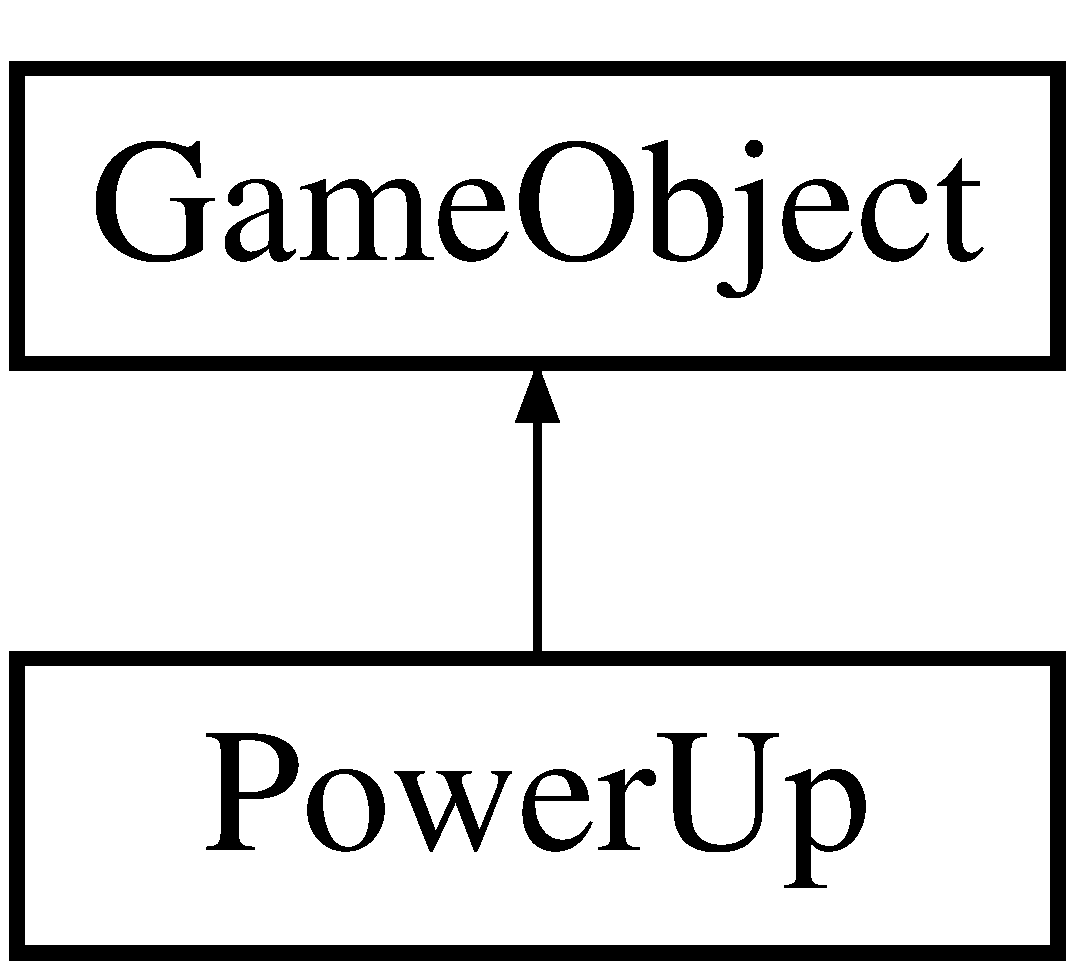
\includegraphics[height=2.000000cm]{class_power_up}
\end{center}
\end{figure}
\subsection*{Public Member Functions}
\begin{DoxyCompactItemize}
\item 
\hyperlink{class_power_up_a46d048ad5911ef25dcf55de24e8dde73}{Power\+Up} (int type, sf\+::\+Vector2f position, sf\+::\+Vector2f size)
\item 
\hyperlink{class_power_up_a353053fe27c5a148a2fcd4f5f45e19af}{$\sim$\+Power\+Up} ()
\item 
void \hyperlink{class_power_up_a3319d56353d0845a1fba25340537d1b9}{initialize\+Color} ()
\item 
void \hyperlink{class_power_up_ab5d07a771930ebeadb6b8b0567436560}{Update} (float dt) override
\item 
void \hyperlink{class_power_up_a0f52fe4ae4e6e47fa3fd4fb2bcc2dcb7}{Draw} (sf\+::\+Render\+Window \&window) override
\item 
void \hyperlink{class_power_up_a4ddb447c9a6bdf1475bc2334590ba55e}{Draw\+With\+X\+Offset} (sf\+::\+Render\+Window \&window, float x\+Offset) override
\item 
void \hyperlink{class_power_up_ad9ec62c1a3832e17949044c8349d0afb}{wrap\+Positions} (\hyperlink{class_camera}{Camera} \&cam) override
\item 
int \hyperlink{class_power_up_aa4c470221625cfabf02a60e2e386f06f}{Get\+Type} ()
\end{DoxyCompactItemize}
\subsection*{Additional Inherited Members}


\subsection{Constructor \& Destructor Documentation}
\hypertarget{class_power_up_a46d048ad5911ef25dcf55de24e8dde73}{}\label{class_power_up_a46d048ad5911ef25dcf55de24e8dde73} 
\index{Power\+Up@{Power\+Up}!Power\+Up@{Power\+Up}}
\index{Power\+Up@{Power\+Up}!Power\+Up@{Power\+Up}}
\subsubsection{\texorpdfstring{Power\+Up()}{PowerUp()}}
{\footnotesize\ttfamily Power\+Up\+::\+Power\+Up (\begin{DoxyParamCaption}\item[{int}]{type,  }\item[{sf\+::\+Vector2f}]{position,  }\item[{sf\+::\+Vector2f}]{size }\end{DoxyParamCaption})}

\hypertarget{class_power_up_a353053fe27c5a148a2fcd4f5f45e19af}{}\label{class_power_up_a353053fe27c5a148a2fcd4f5f45e19af} 
\index{Power\+Up@{Power\+Up}!````~Power\+Up@{$\sim$\+Power\+Up}}
\index{````~Power\+Up@{$\sim$\+Power\+Up}!Power\+Up@{Power\+Up}}
\subsubsection{\texorpdfstring{$\sim$\+Power\+Up()}{~PowerUp()}}
{\footnotesize\ttfamily Power\+Up\+::$\sim$\+Power\+Up (\begin{DoxyParamCaption}{ }\end{DoxyParamCaption})}



\subsection{Member Function Documentation}
\hypertarget{class_power_up_a0f52fe4ae4e6e47fa3fd4fb2bcc2dcb7}{}\label{class_power_up_a0f52fe4ae4e6e47fa3fd4fb2bcc2dcb7} 
\index{Power\+Up@{Power\+Up}!Draw@{Draw}}
\index{Draw@{Draw}!Power\+Up@{Power\+Up}}
\subsubsection{\texorpdfstring{Draw()}{Draw()}}
{\footnotesize\ttfamily void Power\+Up\+::\+Draw (\begin{DoxyParamCaption}\item[{sf\+::\+Render\+Window \&}]{window }\end{DoxyParamCaption})\hspace{0.3cm}{\ttfamily [override]}, {\ttfamily [virtual]}}



Implements \hyperlink{class_game_object_a0bd45eb831b3d0959eb498cad3e412ce}{Game\+Object}.

\hypertarget{class_power_up_a4ddb447c9a6bdf1475bc2334590ba55e}{}\label{class_power_up_a4ddb447c9a6bdf1475bc2334590ba55e} 
\index{Power\+Up@{Power\+Up}!Draw\+With\+X\+Offset@{Draw\+With\+X\+Offset}}
\index{Draw\+With\+X\+Offset@{Draw\+With\+X\+Offset}!Power\+Up@{Power\+Up}}
\subsubsection{\texorpdfstring{Draw\+With\+X\+Offset()}{DrawWithXOffset()}}
{\footnotesize\ttfamily void Power\+Up\+::\+Draw\+With\+X\+Offset (\begin{DoxyParamCaption}\item[{sf\+::\+Render\+Window \&}]{window,  }\item[{float}]{x\+Offset }\end{DoxyParamCaption})\hspace{0.3cm}{\ttfamily [override]}, {\ttfamily [virtual]}}



Implements \hyperlink{class_game_object_a8a3c07e92775fe00baa9e661fefb224e}{Game\+Object}.

\hypertarget{class_power_up_aa4c470221625cfabf02a60e2e386f06f}{}\label{class_power_up_aa4c470221625cfabf02a60e2e386f06f} 
\index{Power\+Up@{Power\+Up}!Get\+Type@{Get\+Type}}
\index{Get\+Type@{Get\+Type}!Power\+Up@{Power\+Up}}
\subsubsection{\texorpdfstring{Get\+Type()}{GetType()}}
{\footnotesize\ttfamily int Power\+Up\+::\+Get\+Type (\begin{DoxyParamCaption}{ }\end{DoxyParamCaption})}

\hypertarget{class_power_up_a3319d56353d0845a1fba25340537d1b9}{}\label{class_power_up_a3319d56353d0845a1fba25340537d1b9} 
\index{Power\+Up@{Power\+Up}!initialize\+Color@{initialize\+Color}}
\index{initialize\+Color@{initialize\+Color}!Power\+Up@{Power\+Up}}
\subsubsection{\texorpdfstring{initialize\+Color()}{initializeColor()}}
{\footnotesize\ttfamily void Power\+Up\+::initialize\+Color (\begin{DoxyParamCaption}{ }\end{DoxyParamCaption})}

\hypertarget{class_power_up_ab5d07a771930ebeadb6b8b0567436560}{}\label{class_power_up_ab5d07a771930ebeadb6b8b0567436560} 
\index{Power\+Up@{Power\+Up}!Update@{Update}}
\index{Update@{Update}!Power\+Up@{Power\+Up}}
\subsubsection{\texorpdfstring{Update()}{Update()}}
{\footnotesize\ttfamily void Power\+Up\+::\+Update (\begin{DoxyParamCaption}\item[{float}]{dt }\end{DoxyParamCaption})\hspace{0.3cm}{\ttfamily [override]}, {\ttfamily [virtual]}}



Implements \hyperlink{class_game_object_a93ed63df640deb516a020530e7f8e045}{Game\+Object}.

\hypertarget{class_power_up_ad9ec62c1a3832e17949044c8349d0afb}{}\label{class_power_up_ad9ec62c1a3832e17949044c8349d0afb} 
\index{Power\+Up@{Power\+Up}!wrap\+Positions@{wrap\+Positions}}
\index{wrap\+Positions@{wrap\+Positions}!Power\+Up@{Power\+Up}}
\subsubsection{\texorpdfstring{wrap\+Positions()}{wrapPositions()}}
{\footnotesize\ttfamily void Power\+Up\+::wrap\+Positions (\begin{DoxyParamCaption}\item[{\hyperlink{class_camera}{Camera} \&}]{cam }\end{DoxyParamCaption})\hspace{0.3cm}{\ttfamily [override]}, {\ttfamily [virtual]}}



Reimplemented from \hyperlink{class_game_object_a53b129d55688652e25e6515d80e669ca}{Game\+Object}.



The documentation for this class was generated from the following files\+:\begin{DoxyCompactItemize}
\item 
Console\+Application2/\hyperlink{_power_up_8h}{Power\+Up.\+h}\item 
Console\+Application2/\hyperlink{_power_up_8cpp}{Power\+Up.\+cpp}\end{DoxyCompactItemize}

\hypertarget{class_power_up_generator}{}\section{Power\+Up\+Generator Class Reference}
\label{class_power_up_generator}\index{Power\+Up\+Generator@{Power\+Up\+Generator}}


{\ttfamily \#include $<$Power\+Up\+Generator.\+h$>$}

\subsection*{Public Member Functions}
\begin{DoxyCompactItemize}
\item 
\hyperlink{class_power_up_generator_af9e9b949330dd6ef6decc758f897454e}{Power\+Up\+Generator} (int powerup\+Type, int min\+Spawn\+Time, int max\+Spawn\+Time)
\item 
\hyperlink{class_power_up_generator_ae2cd842e45e73e0756b93a027ac03207}{$\sim$\+Power\+Up\+Generator} ()
\item 
void \hyperlink{class_power_up_generator_a49002c37923219a8289739b7432e187d}{Update} (float dt)
\end{DoxyCompactItemize}


\subsection{Constructor \& Destructor Documentation}
\hypertarget{class_power_up_generator_af9e9b949330dd6ef6decc758f897454e}{}\label{class_power_up_generator_af9e9b949330dd6ef6decc758f897454e} 
\index{Power\+Up\+Generator@{Power\+Up\+Generator}!Power\+Up\+Generator@{Power\+Up\+Generator}}
\index{Power\+Up\+Generator@{Power\+Up\+Generator}!Power\+Up\+Generator@{Power\+Up\+Generator}}
\subsubsection{\texorpdfstring{Power\+Up\+Generator()}{PowerUpGenerator()}}
{\footnotesize\ttfamily Power\+Up\+Generator\+::\+Power\+Up\+Generator (\begin{DoxyParamCaption}\item[{int}]{powerup\+Type,  }\item[{int}]{min\+Spawn\+Time,  }\item[{int}]{max\+Spawn\+Time }\end{DoxyParamCaption})}

\hypertarget{class_power_up_generator_ae2cd842e45e73e0756b93a027ac03207}{}\label{class_power_up_generator_ae2cd842e45e73e0756b93a027ac03207} 
\index{Power\+Up\+Generator@{Power\+Up\+Generator}!````~Power\+Up\+Generator@{$\sim$\+Power\+Up\+Generator}}
\index{````~Power\+Up\+Generator@{$\sim$\+Power\+Up\+Generator}!Power\+Up\+Generator@{Power\+Up\+Generator}}
\subsubsection{\texorpdfstring{$\sim$\+Power\+Up\+Generator()}{~PowerUpGenerator()}}
{\footnotesize\ttfamily Power\+Up\+Generator\+::$\sim$\+Power\+Up\+Generator (\begin{DoxyParamCaption}{ }\end{DoxyParamCaption})}



\subsection{Member Function Documentation}
\hypertarget{class_power_up_generator_a49002c37923219a8289739b7432e187d}{}\label{class_power_up_generator_a49002c37923219a8289739b7432e187d} 
\index{Power\+Up\+Generator@{Power\+Up\+Generator}!Update@{Update}}
\index{Update@{Update}!Power\+Up\+Generator@{Power\+Up\+Generator}}
\subsubsection{\texorpdfstring{Update()}{Update()}}
{\footnotesize\ttfamily void Power\+Up\+Generator\+::\+Update (\begin{DoxyParamCaption}\item[{float}]{dt }\end{DoxyParamCaption})}



The documentation for this class was generated from the following files\+:\begin{DoxyCompactItemize}
\item 
Console\+Application2/\hyperlink{_power_up_generator_8h}{Power\+Up\+Generator.\+h}\item 
Console\+Application2/\hyperlink{_power_up_generator_8cpp}{Power\+Up\+Generator.\+cpp}\end{DoxyCompactItemize}

\hypertarget{class_power_up_manager}{}\section{Power\+Up\+Manager Class Reference}
\label{class_power_up_manager}\index{Power\+Up\+Manager@{Power\+Up\+Manager}}


{\ttfamily \#include $<$Power\+Up\+Manager.\+h$>$}

\subsection*{Public Member Functions}
\begin{DoxyCompactItemize}
\item 
\hyperlink{class_power_up_manager_a4ef551dbd52ba36cb987a082a92d7eda}{Power\+Up\+Manager} ()
\item 
\hyperlink{class_power_up_manager_a75f5252c97897210c751419d901f8775}{$\sim$\+Power\+Up\+Manager} ()
\item 
void \hyperlink{class_power_up_manager_aa9747a32aa586ad78d4af63f4485f09f}{Add\+Power\+Up\+Generator} (\hyperlink{class_power_up_generator}{Power\+Up\+Generator} $\ast$power\+Up\+Generator)
\item 
void \hyperlink{class_power_up_manager_a07d7f5fdb8c7f38d990ee9f3308430c3}{Update} (float dt)
\end{DoxyCompactItemize}


\subsection{Constructor \& Destructor Documentation}
\hypertarget{class_power_up_manager_a4ef551dbd52ba36cb987a082a92d7eda}{}\label{class_power_up_manager_a4ef551dbd52ba36cb987a082a92d7eda} 
\index{Power\+Up\+Manager@{Power\+Up\+Manager}!Power\+Up\+Manager@{Power\+Up\+Manager}}
\index{Power\+Up\+Manager@{Power\+Up\+Manager}!Power\+Up\+Manager@{Power\+Up\+Manager}}
\subsubsection{\texorpdfstring{Power\+Up\+Manager()}{PowerUpManager()}}
{\footnotesize\ttfamily Power\+Up\+Manager\+::\+Power\+Up\+Manager (\begin{DoxyParamCaption}{ }\end{DoxyParamCaption})}

\hypertarget{class_power_up_manager_a75f5252c97897210c751419d901f8775}{}\label{class_power_up_manager_a75f5252c97897210c751419d901f8775} 
\index{Power\+Up\+Manager@{Power\+Up\+Manager}!````~Power\+Up\+Manager@{$\sim$\+Power\+Up\+Manager}}
\index{````~Power\+Up\+Manager@{$\sim$\+Power\+Up\+Manager}!Power\+Up\+Manager@{Power\+Up\+Manager}}
\subsubsection{\texorpdfstring{$\sim$\+Power\+Up\+Manager()}{~PowerUpManager()}}
{\footnotesize\ttfamily Power\+Up\+Manager\+::$\sim$\+Power\+Up\+Manager (\begin{DoxyParamCaption}{ }\end{DoxyParamCaption})}



\subsection{Member Function Documentation}
\hypertarget{class_power_up_manager_aa9747a32aa586ad78d4af63f4485f09f}{}\label{class_power_up_manager_aa9747a32aa586ad78d4af63f4485f09f} 
\index{Power\+Up\+Manager@{Power\+Up\+Manager}!Add\+Power\+Up\+Generator@{Add\+Power\+Up\+Generator}}
\index{Add\+Power\+Up\+Generator@{Add\+Power\+Up\+Generator}!Power\+Up\+Manager@{Power\+Up\+Manager}}
\subsubsection{\texorpdfstring{Add\+Power\+Up\+Generator()}{AddPowerUpGenerator()}}
{\footnotesize\ttfamily void Power\+Up\+Manager\+::\+Add\+Power\+Up\+Generator (\begin{DoxyParamCaption}\item[{\hyperlink{class_power_up_generator}{Power\+Up\+Generator} $\ast$}]{power\+Up\+Generator }\end{DoxyParamCaption})}

\hypertarget{class_power_up_manager_a07d7f5fdb8c7f38d990ee9f3308430c3}{}\label{class_power_up_manager_a07d7f5fdb8c7f38d990ee9f3308430c3} 
\index{Power\+Up\+Manager@{Power\+Up\+Manager}!Update@{Update}}
\index{Update@{Update}!Power\+Up\+Manager@{Power\+Up\+Manager}}
\subsubsection{\texorpdfstring{Update()}{Update()}}
{\footnotesize\ttfamily void Power\+Up\+Manager\+::\+Update (\begin{DoxyParamCaption}\item[{float}]{dt }\end{DoxyParamCaption})}



The documentation for this class was generated from the following files\+:\begin{DoxyCompactItemize}
\item 
Console\+Application2/\hyperlink{_power_up_manager_8h}{Power\+Up\+Manager.\+h}\item 
Console\+Application2/\hyperlink{_power_up_manager_8cpp}{Power\+Up\+Manager.\+cpp}\end{DoxyCompactItemize}

\hypertarget{class_power_up_types}{}\section{Power\+Up\+Types Class Reference}
\label{class_power_up_types}\index{Power\+Up\+Types@{Power\+Up\+Types}}


{\ttfamily \#include $<$Power\+Up\+Types.\+h$>$}

\subsection*{Public Types}
\begin{DoxyCompactItemize}
\item 
enum \hyperlink{class_power_up_types_a9dd8d899294cc9129d2ed76cd834a3c2}{T\+Y\+P\+ES} \{ \hyperlink{class_power_up_types_a9dd8d899294cc9129d2ed76cd834a3c2af2eb8b16280961a293e62f5a78c70cd3}{H\+Y\+P\+E\+R\+J\+U\+MP}, 
\hyperlink{class_power_up_types_a9dd8d899294cc9129d2ed76cd834a3c2a1592f8286c19e266a7d153f39c9c631d}{M\+O\+R\+E\+\_\+\+F\+I\+R\+E\+\_\+\+R\+A\+TE}, 
\hyperlink{class_power_up_types_a9dd8d899294cc9129d2ed76cd834a3c2a5e487f85188866dc183ef6372a91adaa}{I\+N\+V\+I\+N\+C\+I\+B\+I\+L\+I\+TY}, 
\hyperlink{class_power_up_types_a9dd8d899294cc9129d2ed76cd834a3c2aef2887468841e889dfa02d355bf5197a}{E\+MP}
 \}
\end{DoxyCompactItemize}


\subsection{Member Enumeration Documentation}
\hypertarget{class_power_up_types_a9dd8d899294cc9129d2ed76cd834a3c2}{}\label{class_power_up_types_a9dd8d899294cc9129d2ed76cd834a3c2} 
\index{Power\+Up\+Types@{Power\+Up\+Types}!T\+Y\+P\+ES@{T\+Y\+P\+ES}}
\index{T\+Y\+P\+ES@{T\+Y\+P\+ES}!Power\+Up\+Types@{Power\+Up\+Types}}
\subsubsection{\texorpdfstring{T\+Y\+P\+ES}{TYPES}}
{\footnotesize\ttfamily enum \hyperlink{class_power_up_types_a9dd8d899294cc9129d2ed76cd834a3c2}{Power\+Up\+Types\+::\+T\+Y\+P\+ES}}

\begin{DoxyEnumFields}{Enumerator}
\raisebox{\heightof{T}}[0pt][0pt]{\index{H\+Y\+P\+E\+R\+J\+U\+MP@{H\+Y\+P\+E\+R\+J\+U\+MP}!Power\+Up\+Types@{Power\+Up\+Types}}\index{Power\+Up\+Types@{Power\+Up\+Types}!H\+Y\+P\+E\+R\+J\+U\+MP@{H\+Y\+P\+E\+R\+J\+U\+MP}}}\hypertarget{class_power_up_types_a9dd8d899294cc9129d2ed76cd834a3c2af2eb8b16280961a293e62f5a78c70cd3}{}\label{class_power_up_types_a9dd8d899294cc9129d2ed76cd834a3c2af2eb8b16280961a293e62f5a78c70cd3} 
H\+Y\+P\+E\+R\+J\+U\+MP&\\
\hline

\raisebox{\heightof{T}}[0pt][0pt]{\index{M\+O\+R\+E\+\_\+\+F\+I\+R\+E\+\_\+\+R\+A\+TE@{M\+O\+R\+E\+\_\+\+F\+I\+R\+E\+\_\+\+R\+A\+TE}!Power\+Up\+Types@{Power\+Up\+Types}}\index{Power\+Up\+Types@{Power\+Up\+Types}!M\+O\+R\+E\+\_\+\+F\+I\+R\+E\+\_\+\+R\+A\+TE@{M\+O\+R\+E\+\_\+\+F\+I\+R\+E\+\_\+\+R\+A\+TE}}}\hypertarget{class_power_up_types_a9dd8d899294cc9129d2ed76cd834a3c2a1592f8286c19e266a7d153f39c9c631d}{}\label{class_power_up_types_a9dd8d899294cc9129d2ed76cd834a3c2a1592f8286c19e266a7d153f39c9c631d} 
M\+O\+R\+E\+\_\+\+F\+I\+R\+E\+\_\+\+R\+A\+TE&\\
\hline

\raisebox{\heightof{T}}[0pt][0pt]{\index{I\+N\+V\+I\+N\+C\+I\+B\+I\+L\+I\+TY@{I\+N\+V\+I\+N\+C\+I\+B\+I\+L\+I\+TY}!Power\+Up\+Types@{Power\+Up\+Types}}\index{Power\+Up\+Types@{Power\+Up\+Types}!I\+N\+V\+I\+N\+C\+I\+B\+I\+L\+I\+TY@{I\+N\+V\+I\+N\+C\+I\+B\+I\+L\+I\+TY}}}\hypertarget{class_power_up_types_a9dd8d899294cc9129d2ed76cd834a3c2a5e487f85188866dc183ef6372a91adaa}{}\label{class_power_up_types_a9dd8d899294cc9129d2ed76cd834a3c2a5e487f85188866dc183ef6372a91adaa} 
I\+N\+V\+I\+N\+C\+I\+B\+I\+L\+I\+TY&\\
\hline

\raisebox{\heightof{T}}[0pt][0pt]{\index{E\+MP@{E\+MP}!Power\+Up\+Types@{Power\+Up\+Types}}\index{Power\+Up\+Types@{Power\+Up\+Types}!E\+MP@{E\+MP}}}\hypertarget{class_power_up_types_a9dd8d899294cc9129d2ed76cd834a3c2aef2887468841e889dfa02d355bf5197a}{}\label{class_power_up_types_a9dd8d899294cc9129d2ed76cd834a3c2aef2887468841e889dfa02d355bf5197a} 
E\+MP&\\
\hline

\end{DoxyEnumFields}


The documentation for this class was generated from the following file\+:\begin{DoxyCompactItemize}
\item 
Console\+Application2/\hyperlink{_power_up_types_8h}{Power\+Up\+Types.\+h}\end{DoxyCompactItemize}

\hypertarget{class_rect}{}\section{Rect Class Reference}
\label{class_rect}\index{Rect@{Rect}}


{\ttfamily \#include $<$Simple\+Types.\+h$>$}

\subsection*{Public Member Functions}
\begin{DoxyCompactItemize}
\item 
\hyperlink{class_rect_aa012b316b26079135d9ba828a1330f25}{Rect} (\hyperlink{class_vector2_d}{Vector2D} p, \hyperlink{class_vector2_d}{Vector2D} s)
\item 
\hyperlink{class_rect_aed61433871ffc936171fb1b3b3e3d594}{Rect} (float x=0, float y=0, float w=1, float h=1)
\item 
\hyperlink{class_rect_a5a9cc5f94ff1406c02032bb3676d63e5}{Rect} (sf\+::\+Float\+Rect \&r)
\item 
\hyperlink{class_rect}{Rect} \& \hyperlink{class_rect_a6e26d2923ad8159589fc12e7e857b21a}{operator$\ast$} (float scale)
\item 
\hyperlink{class_rect}{Rect} \& \hyperlink{class_rect_a60d8364198cd7377ebe07ecff6283e49}{operator/} (float scale)
\item 
\hyperlink{class_rect}{Rect} \& \hyperlink{class_rect_a9ceb8cc44e42709056d20d4bbdca15d7}{operator+} (\hyperlink{class_rect}{Rect} \&r)
\item 
\hyperlink{class_vector2_d}{Vector2D} \hyperlink{class_rect_a50af4844d2bd0beb72b75a9890067e43}{get\+Centre\+Copy} ()
\item 
sf\+::\+Rectangle\+Shape \hyperlink{class_rect_a76b9893692559088ccb285e9c3e012c8}{to\+S\+F\+M\+L\+Rect} ()
\item 
bool \hyperlink{class_rect_a81e3d93bf30b2b695058b774f42b4e76}{contains\+Point} (\hyperlink{class_vector2_d}{Vector2D} pt)
\end{DoxyCompactItemize}
\subsection*{Public Attributes}
\begin{DoxyCompactItemize}
\item 
\hyperlink{class_vector2_d}{Vector2D} \hyperlink{class_rect_adb745feadff27b831623019704522ec6}{pos}
\item 
\hyperlink{class_vector2_d}{Vector2D} \hyperlink{class_rect_a1e41d6169d2df56206b3c671480f6e9c}{size}
\end{DoxyCompactItemize}


\subsection{Constructor \& Destructor Documentation}
\hypertarget{class_rect_aa012b316b26079135d9ba828a1330f25}{}\label{class_rect_aa012b316b26079135d9ba828a1330f25} 
\index{Rect@{Rect}!Rect@{Rect}}
\index{Rect@{Rect}!Rect@{Rect}}
\subsubsection{\texorpdfstring{Rect()}{Rect()}\hspace{0.1cm}{\footnotesize\ttfamily [1/3]}}
{\footnotesize\ttfamily Rect\+::\+Rect (\begin{DoxyParamCaption}\item[{\hyperlink{class_vector2_d}{Vector2D}}]{p,  }\item[{\hyperlink{class_vector2_d}{Vector2D}}]{s }\end{DoxyParamCaption})\hspace{0.3cm}{\ttfamily [inline]}}

\hypertarget{class_rect_aed61433871ffc936171fb1b3b3e3d594}{}\label{class_rect_aed61433871ffc936171fb1b3b3e3d594} 
\index{Rect@{Rect}!Rect@{Rect}}
\index{Rect@{Rect}!Rect@{Rect}}
\subsubsection{\texorpdfstring{Rect()}{Rect()}\hspace{0.1cm}{\footnotesize\ttfamily [2/3]}}
{\footnotesize\ttfamily Rect\+::\+Rect (\begin{DoxyParamCaption}\item[{float}]{x = {\ttfamily 0},  }\item[{float}]{y = {\ttfamily 0},  }\item[{float}]{w = {\ttfamily 1},  }\item[{float}]{h = {\ttfamily 1} }\end{DoxyParamCaption})\hspace{0.3cm}{\ttfamily [inline]}}

\hypertarget{class_rect_a5a9cc5f94ff1406c02032bb3676d63e5}{}\label{class_rect_a5a9cc5f94ff1406c02032bb3676d63e5} 
\index{Rect@{Rect}!Rect@{Rect}}
\index{Rect@{Rect}!Rect@{Rect}}
\subsubsection{\texorpdfstring{Rect()}{Rect()}\hspace{0.1cm}{\footnotesize\ttfamily [3/3]}}
{\footnotesize\ttfamily Rect\+::\+Rect (\begin{DoxyParamCaption}\item[{sf\+::\+Float\+Rect \&}]{r }\end{DoxyParamCaption})\hspace{0.3cm}{\ttfamily [inline]}}



\subsection{Member Function Documentation}
\hypertarget{class_rect_a81e3d93bf30b2b695058b774f42b4e76}{}\label{class_rect_a81e3d93bf30b2b695058b774f42b4e76} 
\index{Rect@{Rect}!contains\+Point@{contains\+Point}}
\index{contains\+Point@{contains\+Point}!Rect@{Rect}}
\subsubsection{\texorpdfstring{contains\+Point()}{containsPoint()}}
{\footnotesize\ttfamily bool Rect\+::contains\+Point (\begin{DoxyParamCaption}\item[{\hyperlink{class_vector2_d}{Vector2D}}]{pt }\end{DoxyParamCaption})\hspace{0.3cm}{\ttfamily [inline]}}

\hypertarget{class_rect_a50af4844d2bd0beb72b75a9890067e43}{}\label{class_rect_a50af4844d2bd0beb72b75a9890067e43} 
\index{Rect@{Rect}!get\+Centre\+Copy@{get\+Centre\+Copy}}
\index{get\+Centre\+Copy@{get\+Centre\+Copy}!Rect@{Rect}}
\subsubsection{\texorpdfstring{get\+Centre\+Copy()}{getCentreCopy()}}
{\footnotesize\ttfamily \hyperlink{class_vector2_d}{Vector2D} Rect\+::get\+Centre\+Copy (\begin{DoxyParamCaption}{ }\end{DoxyParamCaption})\hspace{0.3cm}{\ttfamily [inline]}}

\hypertarget{class_rect_a6e26d2923ad8159589fc12e7e857b21a}{}\label{class_rect_a6e26d2923ad8159589fc12e7e857b21a} 
\index{Rect@{Rect}!operator$\ast$@{operator$\ast$}}
\index{operator$\ast$@{operator$\ast$}!Rect@{Rect}}
\subsubsection{\texorpdfstring{operator$\ast$()}{operator*()}}
{\footnotesize\ttfamily \hyperlink{class_rect}{Rect}\& Rect\+::operator$\ast$ (\begin{DoxyParamCaption}\item[{float}]{scale }\end{DoxyParamCaption})\hspace{0.3cm}{\ttfamily [inline]}}

\hypertarget{class_rect_a9ceb8cc44e42709056d20d4bbdca15d7}{}\label{class_rect_a9ceb8cc44e42709056d20d4bbdca15d7} 
\index{Rect@{Rect}!operator+@{operator+}}
\index{operator+@{operator+}!Rect@{Rect}}
\subsubsection{\texorpdfstring{operator+()}{operator+()}}
{\footnotesize\ttfamily \hyperlink{class_rect}{Rect}\& Rect\+::operator+ (\begin{DoxyParamCaption}\item[{\hyperlink{class_rect}{Rect} \&}]{r }\end{DoxyParamCaption})\hspace{0.3cm}{\ttfamily [inline]}}

\hypertarget{class_rect_a60d8364198cd7377ebe07ecff6283e49}{}\label{class_rect_a60d8364198cd7377ebe07ecff6283e49} 
\index{Rect@{Rect}!operator/@{operator/}}
\index{operator/@{operator/}!Rect@{Rect}}
\subsubsection{\texorpdfstring{operator/()}{operator/()}}
{\footnotesize\ttfamily \hyperlink{class_rect}{Rect}\& Rect\+::operator/ (\begin{DoxyParamCaption}\item[{float}]{scale }\end{DoxyParamCaption})\hspace{0.3cm}{\ttfamily [inline]}}

\hypertarget{class_rect_a76b9893692559088ccb285e9c3e012c8}{}\label{class_rect_a76b9893692559088ccb285e9c3e012c8} 
\index{Rect@{Rect}!to\+S\+F\+M\+L\+Rect@{to\+S\+F\+M\+L\+Rect}}
\index{to\+S\+F\+M\+L\+Rect@{to\+S\+F\+M\+L\+Rect}!Rect@{Rect}}
\subsubsection{\texorpdfstring{to\+S\+F\+M\+L\+Rect()}{toSFMLRect()}}
{\footnotesize\ttfamily sf\+::\+Rectangle\+Shape Rect\+::to\+S\+F\+M\+L\+Rect (\begin{DoxyParamCaption}{ }\end{DoxyParamCaption})\hspace{0.3cm}{\ttfamily [inline]}}



\subsection{Member Data Documentation}
\hypertarget{class_rect_adb745feadff27b831623019704522ec6}{}\label{class_rect_adb745feadff27b831623019704522ec6} 
\index{Rect@{Rect}!pos@{pos}}
\index{pos@{pos}!Rect@{Rect}}
\subsubsection{\texorpdfstring{pos}{pos}}
{\footnotesize\ttfamily \hyperlink{class_vector2_d}{Vector2D} Rect\+::pos}

\hypertarget{class_rect_a1e41d6169d2df56206b3c671480f6e9c}{}\label{class_rect_a1e41d6169d2df56206b3c671480f6e9c} 
\index{Rect@{Rect}!size@{size}}
\index{size@{size}!Rect@{Rect}}
\subsubsection{\texorpdfstring{size}{size}}
{\footnotesize\ttfamily \hyperlink{class_vector2_d}{Vector2D} Rect\+::size}



The documentation for this class was generated from the following file\+:\begin{DoxyCompactItemize}
\item 
Console\+Application2/\hyperlink{_simple_types_8h}{Simple\+Types.\+h}\end{DoxyCompactItemize}

\hypertarget{struct_sprite_data}{}\section{Sprite\+Data Struct Reference}
\label{struct_sprite_data}\index{Sprite\+Data@{Sprite\+Data}}


{\ttfamily \#include $<$Asset.\+h$>$}

Inheritance diagram for Sprite\+Data\+:\begin{figure}[H]
\begin{center}
\leavevmode
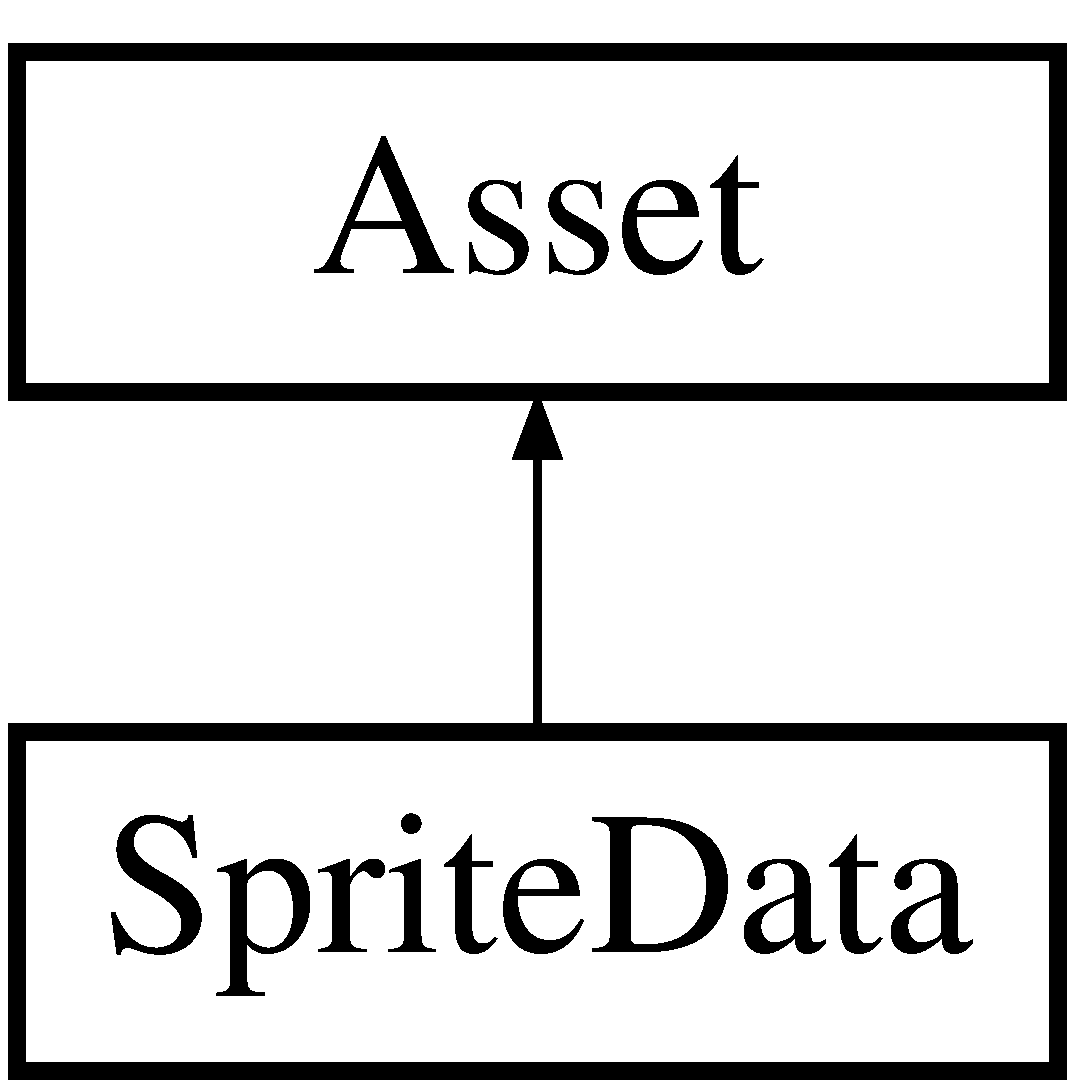
\includegraphics[height=2.000000cm]{struct_sprite_data}
\end{center}
\end{figure}
\subsection*{Public Member Functions}
\begin{DoxyCompactItemize}
\item 
\hyperlink{struct_sprite_data_a8ee6441f4db31fe212c7dd1aba375586}{Sprite\+Data} (string key, string texture\+Dir)
\end{DoxyCompactItemize}
\subsection*{Public Attributes}
\begin{DoxyCompactItemize}
\item 
string \hyperlink{struct_sprite_data_ad855e92487241140b4e283da7d568863}{m\+\_\+texture\+Dir}
\end{DoxyCompactItemize}
\subsection*{Additional Inherited Members}


\subsection{Constructor \& Destructor Documentation}
\hypertarget{struct_sprite_data_a8ee6441f4db31fe212c7dd1aba375586}{}\label{struct_sprite_data_a8ee6441f4db31fe212c7dd1aba375586} 
\index{Sprite\+Data@{Sprite\+Data}!Sprite\+Data@{Sprite\+Data}}
\index{Sprite\+Data@{Sprite\+Data}!Sprite\+Data@{Sprite\+Data}}
\subsubsection{\texorpdfstring{Sprite\+Data()}{SpriteData()}}
{\footnotesize\ttfamily Sprite\+Data\+::\+Sprite\+Data (\begin{DoxyParamCaption}\item[{string}]{key,  }\item[{string}]{texture\+Dir }\end{DoxyParamCaption})\hspace{0.3cm}{\ttfamily [inline]}}



\subsection{Member Data Documentation}
\hypertarget{struct_sprite_data_ad855e92487241140b4e283da7d568863}{}\label{struct_sprite_data_ad855e92487241140b4e283da7d568863} 
\index{Sprite\+Data@{Sprite\+Data}!m\+\_\+texture\+Dir@{m\+\_\+texture\+Dir}}
\index{m\+\_\+texture\+Dir@{m\+\_\+texture\+Dir}!Sprite\+Data@{Sprite\+Data}}
\subsubsection{\texorpdfstring{m\+\_\+texture\+Dir}{m\_textureDir}}
{\footnotesize\ttfamily string Sprite\+Data\+::m\+\_\+texture\+Dir}



The documentation for this struct was generated from the following file\+:\begin{DoxyCompactItemize}
\item 
Console\+Application2/\hyperlink{_asset_8h}{Asset.\+h}\end{DoxyCompactItemize}

\hypertarget{class_terrain}{}\section{Terrain Class Reference}
\label{class_terrain}\index{Terrain@{Terrain}}


{\ttfamily \#include $<$Terrain.\+h$>$}

\subsection*{Static Public Member Functions}
\begin{DoxyCompactItemize}
\item 
static std\+::vector$<$ \hyperlink{class_terrain_segment}{Terrain\+Segment} $\ast$ $>$ \hyperlink{class_terrain_a42a56b23bc25a78d083b8dc3d8da765e}{Generate\+Terrain} (int minY, int maxY, \hyperlink{class_vector2_d}{Vector2D} level\+Size)
\end{DoxyCompactItemize}


\subsection{Member Function Documentation}
\hypertarget{class_terrain_a42a56b23bc25a78d083b8dc3d8da765e}{}\label{class_terrain_a42a56b23bc25a78d083b8dc3d8da765e} 
\index{Terrain@{Terrain}!Generate\+Terrain@{Generate\+Terrain}}
\index{Generate\+Terrain@{Generate\+Terrain}!Terrain@{Terrain}}
\subsubsection{\texorpdfstring{Generate\+Terrain()}{GenerateTerrain()}}
{\footnotesize\ttfamily std\+::vector$<$ \hyperlink{class_terrain_segment}{Terrain\+Segment} $\ast$ $>$ Terrain\+::\+Generate\+Terrain (\begin{DoxyParamCaption}\item[{int}]{minY,  }\item[{int}]{maxY,  }\item[{\hyperlink{class_vector2_d}{Vector2D}}]{level\+Size }\end{DoxyParamCaption})\hspace{0.3cm}{\ttfamily [static]}}



The documentation for this class was generated from the following files\+:\begin{DoxyCompactItemize}
\item 
Console\+Application2/\hyperlink{_terrain_8h}{Terrain.\+h}\item 
Console\+Application2/\hyperlink{_terrain_8cpp}{Terrain.\+cpp}\end{DoxyCompactItemize}

\hypertarget{class_terrain_segment}{}\section{Terrain\+Segment Class Reference}
\label{class_terrain_segment}\index{Terrain\+Segment@{Terrain\+Segment}}


{\ttfamily \#include $<$Terrain\+Segment.\+h$>$}

Inheritance diagram for Terrain\+Segment\+:\begin{figure}[H]
\begin{center}
\leavevmode
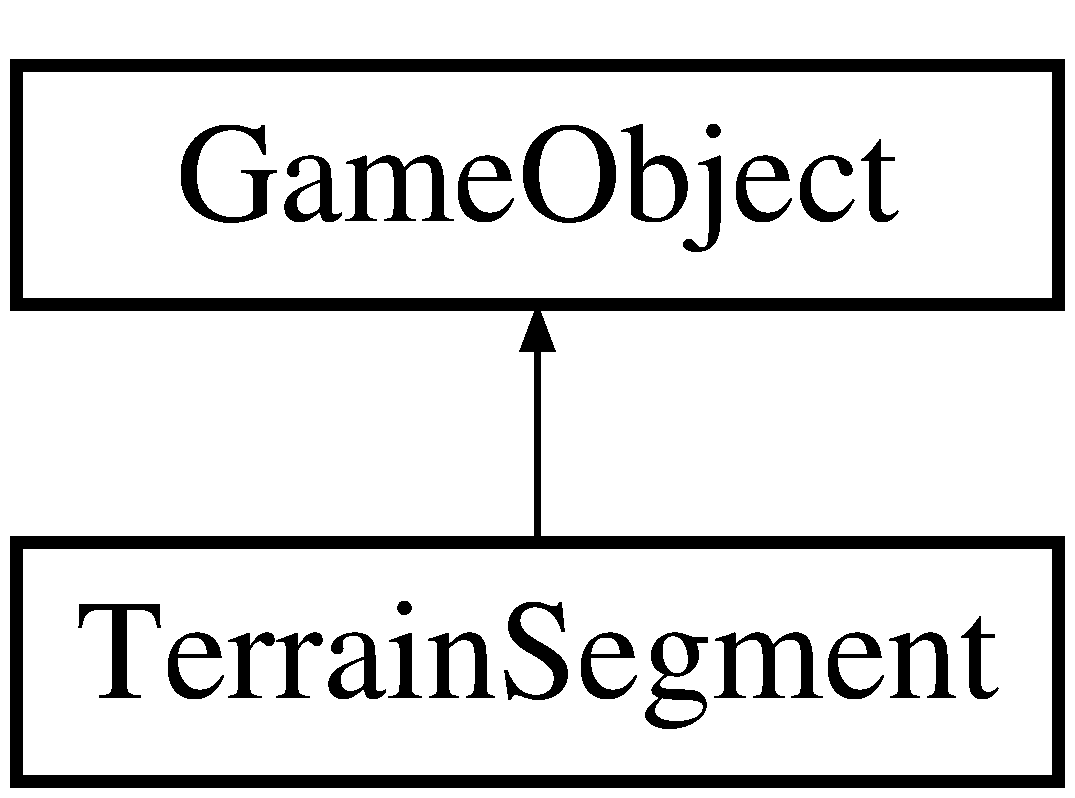
\includegraphics[height=2.000000cm]{class_terrain_segment}
\end{center}
\end{figure}
\subsection*{Public Member Functions}
\begin{DoxyCompactItemize}
\item 
\hyperlink{class_terrain_segment_a01bf8e0e9748e5828425112b74fe9417}{Terrain\+Segment} (sf\+::\+Convex\+Shape shape)
\item 
void \hyperlink{class_terrain_segment_ac8a610b8011a973e775b0cf205ba473a}{Update} (float dt) override
\item 
void \hyperlink{class_terrain_segment_a288c66908f5eaf7974424f64a95d9a9a}{Draw} (sf\+::\+Render\+Window \&window) override
\item 
void \hyperlink{class_terrain_segment_ad9832f83e328b50f647bb844846fb095}{Draw\+With\+X\+Offset} (sf\+::\+Render\+Window \&window, float x\+Offset) override
\end{DoxyCompactItemize}
\subsection*{Additional Inherited Members}


\subsection{Constructor \& Destructor Documentation}
\hypertarget{class_terrain_segment_a01bf8e0e9748e5828425112b74fe9417}{}\label{class_terrain_segment_a01bf8e0e9748e5828425112b74fe9417} 
\index{Terrain\+Segment@{Terrain\+Segment}!Terrain\+Segment@{Terrain\+Segment}}
\index{Terrain\+Segment@{Terrain\+Segment}!Terrain\+Segment@{Terrain\+Segment}}
\subsubsection{\texorpdfstring{Terrain\+Segment()}{TerrainSegment()}}
{\footnotesize\ttfamily Terrain\+Segment\+::\+Terrain\+Segment (\begin{DoxyParamCaption}\item[{sf\+::\+Convex\+Shape}]{shape }\end{DoxyParamCaption})}



\subsection{Member Function Documentation}
\hypertarget{class_terrain_segment_a288c66908f5eaf7974424f64a95d9a9a}{}\label{class_terrain_segment_a288c66908f5eaf7974424f64a95d9a9a} 
\index{Terrain\+Segment@{Terrain\+Segment}!Draw@{Draw}}
\index{Draw@{Draw}!Terrain\+Segment@{Terrain\+Segment}}
\subsubsection{\texorpdfstring{Draw()}{Draw()}}
{\footnotesize\ttfamily void Terrain\+Segment\+::\+Draw (\begin{DoxyParamCaption}\item[{sf\+::\+Render\+Window \&}]{window }\end{DoxyParamCaption})\hspace{0.3cm}{\ttfamily [override]}, {\ttfamily [virtual]}}



Implements \hyperlink{class_game_object_a0bd45eb831b3d0959eb498cad3e412ce}{Game\+Object}.

\hypertarget{class_terrain_segment_ad9832f83e328b50f647bb844846fb095}{}\label{class_terrain_segment_ad9832f83e328b50f647bb844846fb095} 
\index{Terrain\+Segment@{Terrain\+Segment}!Draw\+With\+X\+Offset@{Draw\+With\+X\+Offset}}
\index{Draw\+With\+X\+Offset@{Draw\+With\+X\+Offset}!Terrain\+Segment@{Terrain\+Segment}}
\subsubsection{\texorpdfstring{Draw\+With\+X\+Offset()}{DrawWithXOffset()}}
{\footnotesize\ttfamily void Terrain\+Segment\+::\+Draw\+With\+X\+Offset (\begin{DoxyParamCaption}\item[{sf\+::\+Render\+Window \&}]{window,  }\item[{float}]{x\+Offset }\end{DoxyParamCaption})\hspace{0.3cm}{\ttfamily [override]}, {\ttfamily [virtual]}}



Implements \hyperlink{class_game_object_a8a3c07e92775fe00baa9e661fefb224e}{Game\+Object}.

\hypertarget{class_terrain_segment_ac8a610b8011a973e775b0cf205ba473a}{}\label{class_terrain_segment_ac8a610b8011a973e775b0cf205ba473a} 
\index{Terrain\+Segment@{Terrain\+Segment}!Update@{Update}}
\index{Update@{Update}!Terrain\+Segment@{Terrain\+Segment}}
\subsubsection{\texorpdfstring{Update()}{Update()}}
{\footnotesize\ttfamily void Terrain\+Segment\+::\+Update (\begin{DoxyParamCaption}\item[{float}]{dt }\end{DoxyParamCaption})\hspace{0.3cm}{\ttfamily [override]}, {\ttfamily [virtual]}}



Implements \hyperlink{class_game_object_a93ed63df640deb516a020530e7f8e045}{Game\+Object}.



The documentation for this class was generated from the following files\+:\begin{DoxyCompactItemize}
\item 
Console\+Application2/\hyperlink{_terrain_segment_8h}{Terrain\+Segment.\+h}\item 
Console\+Application2/\hyperlink{_terrain_segment_8cpp}{Terrain\+Segment.\+cpp}\end{DoxyCompactItemize}

\hypertarget{class_vector2_d}{}\section{Vector2D Class Reference}
\label{class_vector2_d}\index{Vector2D@{Vector2D}}


{\ttfamily \#include $<$Vector2\+D.\+h$>$}

\subsection*{Public Member Functions}
\begin{DoxyCompactItemize}
\item 
\hyperlink{class_vector2_d_a519c8120da5581b006fba4d01b243bc1}{$\sim$\+Vector2D} (void)
\item 
\hyperlink{class_vector2_d_a98e9997ebb7a629f4db52397d4e0d653}{Vector2D} ()
\item 
\hyperlink{class_vector2_d_a98cb7602bcb90bbb11b6bb99b3647f1a}{Vector2D} (sf\+::\+Vector2f v)
\item 
\hyperlink{class_vector2_d_ac8545dc4359145ab643ccc88758c9162}{Vector2D} (float angle)
\item 
\hyperlink{class_vector2_d_aadcb679a8c3fd6eaad3418d9df5f7529}{Vector2D} (float, float)
\item 
sf\+::\+Vector2f \hyperlink{class_vector2_d_ad586df868be4520798c5783e317adbeb}{to\+S\+F\+M\+L\+Vector} ()
\item 
\hyperlink{class_vector2_d_a68c8555c932b512c1b371e76c5ee9698}{Vector2D} (const \hyperlink{class_vector2_d}{Vector2D} \&v)
\item 
void \hyperlink{class_vector2_d_afa1ae9e0f8f050504007fe93c72c9ae7}{limit} (float max\+Magnitude)
\item 
\hyperlink{class_vector2_d}{Vector2D} \hyperlink{class_vector2_d_a7d3aaf8b43dab548e9fc8ae62101bacf}{operator+} (const \hyperlink{class_vector2_d}{Vector2D} \&) const
\item 
\hyperlink{class_vector2_d}{Vector2D} \hyperlink{class_vector2_d_ac5aba3d5d2a7bd57ef847e153fad739e}{operator-\/} (const \hyperlink{class_vector2_d}{Vector2D} \&) const
\item 
\hyperlink{class_vector2_d}{Vector2D} \hyperlink{class_vector2_d_a120fd7fe91b4399bd3034196b3ecb66d}{operator$\ast$} (const \hyperlink{class_vector2_d}{Vector2D} \&) const
\item 
\hyperlink{class_vector2_d}{Vector2D} \hyperlink{class_vector2_d_aa8f1dbcedc16fa35320e9a5bf50e78b1}{operator/} (const \hyperlink{class_vector2_d}{Vector2D} \&) const
\item 
\hyperlink{class_vector2_d}{Vector2D} \hyperlink{class_vector2_d_a1e0134bc5942c384eb6f6a6c7b7ab62c}{operator+=} (const \hyperlink{class_vector2_d}{Vector2D} \&)
\item 
\hyperlink{class_vector2_d}{Vector2D} \hyperlink{class_vector2_d_af4f02654807e191cd084d2795b2037ce}{operator=} (const \hyperlink{class_vector2_d}{Vector2D} \&v)
\item 
\hyperlink{class_vector2_d}{Vector2D} \hyperlink{class_vector2_d_af699c21f9bd8ac3a30c6defa171ca94d}{Normalize} ()
\item 
bool \hyperlink{class_vector2_d_a85f309a7b1e82760d2524b7cc8896ef7}{operator==} (const \hyperlink{class_vector2_d}{Vector2D} \&) const
\item 
bool \hyperlink{class_vector2_d_afd5e33bd705b64c6b5d9dc02ff210a65}{operator$>$} (const \hyperlink{class_vector2_d}{Vector2D} \&) const
\item 
bool \hyperlink{class_vector2_d_aa6e719e5a3b752156bbe6879c7ae57d5}{operator$<$} (const \hyperlink{class_vector2_d}{Vector2D} \&) const
\item 
bool \hyperlink{class_vector2_d_a5f4ccbfffd4e05947cae418a5c038352}{operator$>$=} (const \hyperlink{class_vector2_d}{Vector2D} \&) const
\item 
bool \hyperlink{class_vector2_d_a3be8fe1d7c8f70e14fd2cc65a49b9b22}{operator$<$=} (const \hyperlink{class_vector2_d}{Vector2D} \&) const
\item 
\hyperlink{class_vector2_d}{Vector2D} \hyperlink{class_vector2_d_af2f279f4de17d3d3ae69b476cf6ac945}{operator-\/} () const
\item 
\hyperlink{class_vector2_d}{Vector2D} \hyperlink{class_vector2_d_a8eba32059605848ce2357b57ec903e06}{operator=} (const sf\+::\+Vector2f \&)
\item 
\hyperlink{class_vector2_d}{Vector2D} \hyperlink{class_vector2_d_ab4f9db2da060af72008c10622efb07bd}{operator$\ast$} (const float \&) const
\item 
\hyperlink{class_vector2_d}{Vector2D} \hyperlink{class_vector2_d_a48e182885509ad31beb12ebda25fdbae}{operator/} (const float \&) const
\item 
float \hyperlink{class_vector2_d_a4c09243b446e694ef66788eeadd14627}{Dot\+Product} (const \hyperlink{class_vector2_d}{Vector2D} \&)
\item 
float \hyperlink{class_vector2_d_afaa1e7b4e83f8e407dc83837349febe3}{Magnitude} ()
\end{DoxyCompactItemize}
\subsection*{Static Public Member Functions}
\begin{DoxyCompactItemize}
\item 
static \hyperlink{class_vector2_d}{Vector2D} \hyperlink{class_vector2_d_ae6670477c183fef0006d0af7f9b8ee09}{Normalize} (\hyperlink{class_vector2_d}{Vector2D} t)
\item 
static \hyperlink{class_vector2_d}{Vector2D} \hyperlink{class_vector2_d_a483b380a98091be25a4ac092eb42ee0f}{Direction\+Vector\+Between\+Two\+Points} (const \hyperlink{class_vector2_d}{Vector2D} \&, const \hyperlink{class_vector2_d}{Vector2D} \&)
\item 
static float \hyperlink{class_vector2_d_af901712cb8cb175c42eed90415cfd214}{Dot\+Product} (const \hyperlink{class_vector2_d}{Vector2D} \&, const \hyperlink{class_vector2_d}{Vector2D} \&)
\item 
static float \hyperlink{class_vector2_d_ad9557501f1291b4be24d940483754a4b}{Cross\+Product} (const \hyperlink{class_vector2_d}{Vector2D} \&, const \hyperlink{class_vector2_d}{Vector2D} \&)
\item 
static float \hyperlink{class_vector2_d_ab4ba105fdb95eed5a9bdd0137fe1ac13}{Magnitude} (const \hyperlink{class_vector2_d}{Vector2D} \&)
\item 
static \hyperlink{class_vector2_d}{Vector2D} \hyperlink{class_vector2_d_ac7936ba558378f5a558ca9954303e72c}{Normal} (const \hyperlink{class_vector2_d}{Vector2D} \&)
\item 
static \hyperlink{class_vector2_d}{Vector2D} \hyperlink{class_vector2_d_a283016b326b61db46c85ca1df8530d50}{Perpendicular} (const \hyperlink{class_vector2_d}{Vector2D} \&)
\item 
static bool \hyperlink{class_vector2_d_ae18bd72a2e20265772884cbf7a9bff94}{Intersect} (const \hyperlink{class_vector2_d}{Vector2D} \&, const \hyperlink{class_vector2_d}{Vector2D} \&, const \hyperlink{class_vector2_d}{Vector2D} \&, const \hyperlink{class_vector2_d}{Vector2D} \&)
\item 
static \hyperlink{class_vector2_d}{Vector2D} \hyperlink{class_vector2_d_a61b8609e60892e34d458559ec11d020a}{Get\+Intersect} (const \hyperlink{class_vector2_d}{Vector2D} \&, const \hyperlink{class_vector2_d}{Vector2D} \&, const \hyperlink{class_vector2_d}{Vector2D} \&, const \hyperlink{class_vector2_d}{Vector2D} \&)
\item 
static float \hyperlink{class_vector2_d_a93592066c13a15a9f244ebccc04134ec}{Distance} (\hyperlink{class_vector2_d}{Vector2D} \&one, \hyperlink{class_vector2_d}{Vector2D} \&two)
\item 
static float \hyperlink{class_vector2_d_ad76081cba5229267c50aeb3e92ca1f1c}{Distance\+Sq} (\hyperlink{class_vector2_d}{Vector2D} \&one, \hyperlink{class_vector2_d}{Vector2D} \&two)
\item 
static float \hyperlink{class_vector2_d_aa406360b37523a1ddae7685330a1f53e}{Angle\+Deg} (\hyperlink{class_vector2_d}{Vector2D} \&one, \hyperlink{class_vector2_d}{Vector2D} \&two)
\item 
static float \hyperlink{class_vector2_d_a9d109b3c593fd52b42014c85149c9fe5}{Angle\+Rad} (\hyperlink{class_vector2_d}{Vector2D} \&one, \hyperlink{class_vector2_d}{Vector2D} \&two)
\end{DoxyCompactItemize}
\subsection*{Public Attributes}
\begin{DoxyCompactItemize}
\item 
float \hyperlink{class_vector2_d_aeb4253ba6555251d010ea4450619029e}{x}
\item 
float \& \hyperlink{class_vector2_d_a849dfb5d61bc6500e259011f512188e3}{width} = \hyperlink{class_vector2_d_aeb4253ba6555251d010ea4450619029e}{x}
\item 
float \& \hyperlink{class_vector2_d_a855db1822aebf50dd1521a1a550a30b8}{w} = \hyperlink{class_vector2_d_aeb4253ba6555251d010ea4450619029e}{x}
\item 
float \hyperlink{class_vector2_d_a85215519d3f71d0e6be7d636346f3b7d}{y}
\item 
float \& \hyperlink{class_vector2_d_a725dfed5745aa8176cd39ae334536bae}{height} = \hyperlink{class_vector2_d_a85215519d3f71d0e6be7d636346f3b7d}{y}
\item 
float \& \hyperlink{class_vector2_d_a8de2b56d13d0f0a7f9357dc42eef731e}{h} = \hyperlink{class_vector2_d_a85215519d3f71d0e6be7d636346f3b7d}{y}
\end{DoxyCompactItemize}
\subsection*{Static Public Attributes}
\begin{DoxyCompactItemize}
\item 
static const \hyperlink{class_vector2_d}{Vector2D} \hyperlink{class_vector2_d_abd688d20c24b9d6fca4378e3c65e37dc}{UP} = \hyperlink{class_vector2_d}{Vector2D}(0, -\/1)
\item 
static const \hyperlink{class_vector2_d}{Vector2D} \hyperlink{class_vector2_d_a88282ec1acd645ccd8195c9c624c2607}{L\+E\+FT} = \hyperlink{class_vector2_d}{Vector2D}(-\/1, 0)
\item 
static const \hyperlink{class_vector2_d}{Vector2D} \hyperlink{class_vector2_d_a7c995f75e1c94be2be0d4cc930dad709}{D\+O\+WN} = \hyperlink{class_vector2_d}{Vector2D}(0, 1)
\item 
static const \hyperlink{class_vector2_d}{Vector2D} \hyperlink{class_vector2_d_a066be8679c3ac8b38a42b3384aadf76f}{R\+I\+G\+HT} = \hyperlink{class_vector2_d}{Vector2D}(1, 0)
\item 
static const \hyperlink{class_vector2_d}{Vector2D} \hyperlink{class_vector2_d_ab9f4481b021711cbbd4ec78390aa1e6e}{Z\+E\+RO} = \hyperlink{class_vector2_d}{Vector2D}(0, 0)
\end{DoxyCompactItemize}


\subsection{Constructor \& Destructor Documentation}
\hypertarget{class_vector2_d_a519c8120da5581b006fba4d01b243bc1}{}\label{class_vector2_d_a519c8120da5581b006fba4d01b243bc1} 
\index{Vector2D@{Vector2D}!````~Vector2D@{$\sim$\+Vector2D}}
\index{````~Vector2D@{$\sim$\+Vector2D}!Vector2D@{Vector2D}}
\subsubsection{\texorpdfstring{$\sim$\+Vector2\+D()}{~Vector2D()}}
{\footnotesize\ttfamily Vector2\+D\+::$\sim$\+Vector2D (\begin{DoxyParamCaption}\item[{void}]{ }\end{DoxyParamCaption})}

\hypertarget{class_vector2_d_a98e9997ebb7a629f4db52397d4e0d653}{}\label{class_vector2_d_a98e9997ebb7a629f4db52397d4e0d653} 
\index{Vector2D@{Vector2D}!Vector2D@{Vector2D}}
\index{Vector2D@{Vector2D}!Vector2D@{Vector2D}}
\subsubsection{\texorpdfstring{Vector2\+D()}{Vector2D()}\hspace{0.1cm}{\footnotesize\ttfamily [1/5]}}
{\footnotesize\ttfamily Vector2\+D\+::\+Vector2D (\begin{DoxyParamCaption}{ }\end{DoxyParamCaption})}

\hypertarget{class_vector2_d_a98cb7602bcb90bbb11b6bb99b3647f1a}{}\label{class_vector2_d_a98cb7602bcb90bbb11b6bb99b3647f1a} 
\index{Vector2D@{Vector2D}!Vector2D@{Vector2D}}
\index{Vector2D@{Vector2D}!Vector2D@{Vector2D}}
\subsubsection{\texorpdfstring{Vector2\+D()}{Vector2D()}\hspace{0.1cm}{\footnotesize\ttfamily [2/5]}}
{\footnotesize\ttfamily Vector2\+D\+::\+Vector2D (\begin{DoxyParamCaption}\item[{sf\+::\+Vector2f}]{v }\end{DoxyParamCaption})}

\hypertarget{class_vector2_d_ac8545dc4359145ab643ccc88758c9162}{}\label{class_vector2_d_ac8545dc4359145ab643ccc88758c9162} 
\index{Vector2D@{Vector2D}!Vector2D@{Vector2D}}
\index{Vector2D@{Vector2D}!Vector2D@{Vector2D}}
\subsubsection{\texorpdfstring{Vector2\+D()}{Vector2D()}\hspace{0.1cm}{\footnotesize\ttfamily [3/5]}}
{\footnotesize\ttfamily Vector2\+D\+::\+Vector2D (\begin{DoxyParamCaption}\item[{float}]{angle }\end{DoxyParamCaption})}

\hypertarget{class_vector2_d_aadcb679a8c3fd6eaad3418d9df5f7529}{}\label{class_vector2_d_aadcb679a8c3fd6eaad3418d9df5f7529} 
\index{Vector2D@{Vector2D}!Vector2D@{Vector2D}}
\index{Vector2D@{Vector2D}!Vector2D@{Vector2D}}
\subsubsection{\texorpdfstring{Vector2\+D()}{Vector2D()}\hspace{0.1cm}{\footnotesize\ttfamily [4/5]}}
{\footnotesize\ttfamily Vector2\+D\+::\+Vector2D (\begin{DoxyParamCaption}\item[{float}]{sourceX,  }\item[{float}]{sourceY }\end{DoxyParamCaption})}

\hypertarget{class_vector2_d_a68c8555c932b512c1b371e76c5ee9698}{}\label{class_vector2_d_a68c8555c932b512c1b371e76c5ee9698} 
\index{Vector2D@{Vector2D}!Vector2D@{Vector2D}}
\index{Vector2D@{Vector2D}!Vector2D@{Vector2D}}
\subsubsection{\texorpdfstring{Vector2\+D()}{Vector2D()}\hspace{0.1cm}{\footnotesize\ttfamily [5/5]}}
{\footnotesize\ttfamily Vector2\+D\+::\+Vector2D (\begin{DoxyParamCaption}\item[{const \hyperlink{class_vector2_d}{Vector2D} \&}]{v }\end{DoxyParamCaption})}



\subsection{Member Function Documentation}
\hypertarget{class_vector2_d_aa406360b37523a1ddae7685330a1f53e}{}\label{class_vector2_d_aa406360b37523a1ddae7685330a1f53e} 
\index{Vector2D@{Vector2D}!Angle\+Deg@{Angle\+Deg}}
\index{Angle\+Deg@{Angle\+Deg}!Vector2D@{Vector2D}}
\subsubsection{\texorpdfstring{Angle\+Deg()}{AngleDeg()}}
{\footnotesize\ttfamily float Vector2\+D\+::\+Angle\+Deg (\begin{DoxyParamCaption}\item[{\hyperlink{class_vector2_d}{Vector2D} \&}]{one,  }\item[{\hyperlink{class_vector2_d}{Vector2D} \&}]{two }\end{DoxyParamCaption})\hspace{0.3cm}{\ttfamily [static]}}

\hypertarget{class_vector2_d_a9d109b3c593fd52b42014c85149c9fe5}{}\label{class_vector2_d_a9d109b3c593fd52b42014c85149c9fe5} 
\index{Vector2D@{Vector2D}!Angle\+Rad@{Angle\+Rad}}
\index{Angle\+Rad@{Angle\+Rad}!Vector2D@{Vector2D}}
\subsubsection{\texorpdfstring{Angle\+Rad()}{AngleRad()}}
{\footnotesize\ttfamily float Vector2\+D\+::\+Angle\+Rad (\begin{DoxyParamCaption}\item[{\hyperlink{class_vector2_d}{Vector2D} \&}]{one,  }\item[{\hyperlink{class_vector2_d}{Vector2D} \&}]{two }\end{DoxyParamCaption})\hspace{0.3cm}{\ttfamily [static]}}

\hypertarget{class_vector2_d_ad9557501f1291b4be24d940483754a4b}{}\label{class_vector2_d_ad9557501f1291b4be24d940483754a4b} 
\index{Vector2D@{Vector2D}!Cross\+Product@{Cross\+Product}}
\index{Cross\+Product@{Cross\+Product}!Vector2D@{Vector2D}}
\subsubsection{\texorpdfstring{Cross\+Product()}{CrossProduct()}}
{\footnotesize\ttfamily float Vector2\+D\+::\+Cross\+Product (\begin{DoxyParamCaption}\item[{const \hyperlink{class_vector2_d}{Vector2D} \&}]{a,  }\item[{const \hyperlink{class_vector2_d}{Vector2D} \&}]{b }\end{DoxyParamCaption})\hspace{0.3cm}{\ttfamily [static]}}

\hypertarget{class_vector2_d_a483b380a98091be25a4ac092eb42ee0f}{}\label{class_vector2_d_a483b380a98091be25a4ac092eb42ee0f} 
\index{Vector2D@{Vector2D}!Direction\+Vector\+Between\+Two\+Points@{Direction\+Vector\+Between\+Two\+Points}}
\index{Direction\+Vector\+Between\+Two\+Points@{Direction\+Vector\+Between\+Two\+Points}!Vector2D@{Vector2D}}
\subsubsection{\texorpdfstring{Direction\+Vector\+Between\+Two\+Points()}{DirectionVectorBetweenTwoPoints()}}
{\footnotesize\ttfamily \hyperlink{class_vector2_d}{Vector2D} Vector2\+D\+::\+Direction\+Vector\+Between\+Two\+Points (\begin{DoxyParamCaption}\item[{const \hyperlink{class_vector2_d}{Vector2D} \&}]{v1,  }\item[{const \hyperlink{class_vector2_d}{Vector2D} \&}]{v2 }\end{DoxyParamCaption})\hspace{0.3cm}{\ttfamily [static]}}

\hypertarget{class_vector2_d_a93592066c13a15a9f244ebccc04134ec}{}\label{class_vector2_d_a93592066c13a15a9f244ebccc04134ec} 
\index{Vector2D@{Vector2D}!Distance@{Distance}}
\index{Distance@{Distance}!Vector2D@{Vector2D}}
\subsubsection{\texorpdfstring{Distance()}{Distance()}}
{\footnotesize\ttfamily float Vector2\+D\+::\+Distance (\begin{DoxyParamCaption}\item[{\hyperlink{class_vector2_d}{Vector2D} \&}]{one,  }\item[{\hyperlink{class_vector2_d}{Vector2D} \&}]{two }\end{DoxyParamCaption})\hspace{0.3cm}{\ttfamily [static]}}

\hypertarget{class_vector2_d_ad76081cba5229267c50aeb3e92ca1f1c}{}\label{class_vector2_d_ad76081cba5229267c50aeb3e92ca1f1c} 
\index{Vector2D@{Vector2D}!Distance\+Sq@{Distance\+Sq}}
\index{Distance\+Sq@{Distance\+Sq}!Vector2D@{Vector2D}}
\subsubsection{\texorpdfstring{Distance\+Sq()}{DistanceSq()}}
{\footnotesize\ttfamily float Vector2\+D\+::\+Distance\+Sq (\begin{DoxyParamCaption}\item[{\hyperlink{class_vector2_d}{Vector2D} \&}]{one,  }\item[{\hyperlink{class_vector2_d}{Vector2D} \&}]{two }\end{DoxyParamCaption})\hspace{0.3cm}{\ttfamily [static]}}

\hypertarget{class_vector2_d_af901712cb8cb175c42eed90415cfd214}{}\label{class_vector2_d_af901712cb8cb175c42eed90415cfd214} 
\index{Vector2D@{Vector2D}!Dot\+Product@{Dot\+Product}}
\index{Dot\+Product@{Dot\+Product}!Vector2D@{Vector2D}}
\subsubsection{\texorpdfstring{Dot\+Product()}{DotProduct()}\hspace{0.1cm}{\footnotesize\ttfamily [1/2]}}
{\footnotesize\ttfamily float Vector2\+D\+::\+Dot\+Product (\begin{DoxyParamCaption}\item[{const \hyperlink{class_vector2_d}{Vector2D} \&}]{a,  }\item[{const \hyperlink{class_vector2_d}{Vector2D} \&}]{b }\end{DoxyParamCaption})\hspace{0.3cm}{\ttfamily [static]}}

\hypertarget{class_vector2_d_a4c09243b446e694ef66788eeadd14627}{}\label{class_vector2_d_a4c09243b446e694ef66788eeadd14627} 
\index{Vector2D@{Vector2D}!Dot\+Product@{Dot\+Product}}
\index{Dot\+Product@{Dot\+Product}!Vector2D@{Vector2D}}
\subsubsection{\texorpdfstring{Dot\+Product()}{DotProduct()}\hspace{0.1cm}{\footnotesize\ttfamily [2/2]}}
{\footnotesize\ttfamily float Vector2\+D\+::\+Dot\+Product (\begin{DoxyParamCaption}\item[{const \hyperlink{class_vector2_d}{Vector2D} \&}]{b }\end{DoxyParamCaption})}

\hypertarget{class_vector2_d_a61b8609e60892e34d458559ec11d020a}{}\label{class_vector2_d_a61b8609e60892e34d458559ec11d020a} 
\index{Vector2D@{Vector2D}!Get\+Intersect@{Get\+Intersect}}
\index{Get\+Intersect@{Get\+Intersect}!Vector2D@{Vector2D}}
\subsubsection{\texorpdfstring{Get\+Intersect()}{GetIntersect()}}
{\footnotesize\ttfamily \hyperlink{class_vector2_d}{Vector2D} Vector2\+D\+::\+Get\+Intersect (\begin{DoxyParamCaption}\item[{const \hyperlink{class_vector2_d}{Vector2D} \&}]{aa,  }\item[{const \hyperlink{class_vector2_d}{Vector2D} \&}]{ab,  }\item[{const \hyperlink{class_vector2_d}{Vector2D} \&}]{ba,  }\item[{const \hyperlink{class_vector2_d}{Vector2D} \&}]{bb }\end{DoxyParamCaption})\hspace{0.3cm}{\ttfamily [static]}}

\hypertarget{class_vector2_d_ae18bd72a2e20265772884cbf7a9bff94}{}\label{class_vector2_d_ae18bd72a2e20265772884cbf7a9bff94} 
\index{Vector2D@{Vector2D}!Intersect@{Intersect}}
\index{Intersect@{Intersect}!Vector2D@{Vector2D}}
\subsubsection{\texorpdfstring{Intersect()}{Intersect()}}
{\footnotesize\ttfamily bool Vector2\+D\+::\+Intersect (\begin{DoxyParamCaption}\item[{const \hyperlink{class_vector2_d}{Vector2D} \&}]{aa,  }\item[{const \hyperlink{class_vector2_d}{Vector2D} \&}]{ab,  }\item[{const \hyperlink{class_vector2_d}{Vector2D} \&}]{ba,  }\item[{const \hyperlink{class_vector2_d}{Vector2D} \&}]{bb }\end{DoxyParamCaption})\hspace{0.3cm}{\ttfamily [static]}}

\hypertarget{class_vector2_d_afa1ae9e0f8f050504007fe93c72c9ae7}{}\label{class_vector2_d_afa1ae9e0f8f050504007fe93c72c9ae7} 
\index{Vector2D@{Vector2D}!limit@{limit}}
\index{limit@{limit}!Vector2D@{Vector2D}}
\subsubsection{\texorpdfstring{limit()}{limit()}}
{\footnotesize\ttfamily void Vector2\+D\+::limit (\begin{DoxyParamCaption}\item[{float}]{max\+Magnitude }\end{DoxyParamCaption})}

\hypertarget{class_vector2_d_ab4ba105fdb95eed5a9bdd0137fe1ac13}{}\label{class_vector2_d_ab4ba105fdb95eed5a9bdd0137fe1ac13} 
\index{Vector2D@{Vector2D}!Magnitude@{Magnitude}}
\index{Magnitude@{Magnitude}!Vector2D@{Vector2D}}
\subsubsection{\texorpdfstring{Magnitude()}{Magnitude()}\hspace{0.1cm}{\footnotesize\ttfamily [1/2]}}
{\footnotesize\ttfamily float Vector2\+D\+::\+Magnitude (\begin{DoxyParamCaption}\item[{const \hyperlink{class_vector2_d}{Vector2D} \&}]{v }\end{DoxyParamCaption})\hspace{0.3cm}{\ttfamily [static]}}

\hypertarget{class_vector2_d_afaa1e7b4e83f8e407dc83837349febe3}{}\label{class_vector2_d_afaa1e7b4e83f8e407dc83837349febe3} 
\index{Vector2D@{Vector2D}!Magnitude@{Magnitude}}
\index{Magnitude@{Magnitude}!Vector2D@{Vector2D}}
\subsubsection{\texorpdfstring{Magnitude()}{Magnitude()}\hspace{0.1cm}{\footnotesize\ttfamily [2/2]}}
{\footnotesize\ttfamily float Vector2\+D\+::\+Magnitude (\begin{DoxyParamCaption}{ }\end{DoxyParamCaption})}

\hypertarget{class_vector2_d_ac7936ba558378f5a558ca9954303e72c}{}\label{class_vector2_d_ac7936ba558378f5a558ca9954303e72c} 
\index{Vector2D@{Vector2D}!Normal@{Normal}}
\index{Normal@{Normal}!Vector2D@{Vector2D}}
\subsubsection{\texorpdfstring{Normal()}{Normal()}}
{\footnotesize\ttfamily \hyperlink{class_vector2_d}{Vector2D} Vector2\+D\+::\+Normal (\begin{DoxyParamCaption}\item[{const \hyperlink{class_vector2_d}{Vector2D} \&}]{v }\end{DoxyParamCaption})\hspace{0.3cm}{\ttfamily [static]}}

\hypertarget{class_vector2_d_af699c21f9bd8ac3a30c6defa171ca94d}{}\label{class_vector2_d_af699c21f9bd8ac3a30c6defa171ca94d} 
\index{Vector2D@{Vector2D}!Normalize@{Normalize}}
\index{Normalize@{Normalize}!Vector2D@{Vector2D}}
\subsubsection{\texorpdfstring{Normalize()}{Normalize()}\hspace{0.1cm}{\footnotesize\ttfamily [1/2]}}
{\footnotesize\ttfamily \hyperlink{class_vector2_d}{Vector2D} Vector2\+D\+::\+Normalize (\begin{DoxyParamCaption}{ }\end{DoxyParamCaption})}

\hypertarget{class_vector2_d_ae6670477c183fef0006d0af7f9b8ee09}{}\label{class_vector2_d_ae6670477c183fef0006d0af7f9b8ee09} 
\index{Vector2D@{Vector2D}!Normalize@{Normalize}}
\index{Normalize@{Normalize}!Vector2D@{Vector2D}}
\subsubsection{\texorpdfstring{Normalize()}{Normalize()}\hspace{0.1cm}{\footnotesize\ttfamily [2/2]}}
{\footnotesize\ttfamily \hyperlink{class_vector2_d}{Vector2D} Vector2\+D\+::\+Normalize (\begin{DoxyParamCaption}\item[{\hyperlink{class_vector2_d}{Vector2D}}]{t }\end{DoxyParamCaption})\hspace{0.3cm}{\ttfamily [static]}}

\hypertarget{class_vector2_d_a120fd7fe91b4399bd3034196b3ecb66d}{}\label{class_vector2_d_a120fd7fe91b4399bd3034196b3ecb66d} 
\index{Vector2D@{Vector2D}!operator$\ast$@{operator$\ast$}}
\index{operator$\ast$@{operator$\ast$}!Vector2D@{Vector2D}}
\subsubsection{\texorpdfstring{operator$\ast$()}{operator*()}\hspace{0.1cm}{\footnotesize\ttfamily [1/2]}}
{\footnotesize\ttfamily \hyperlink{class_vector2_d}{Vector2D} Vector2\+D\+::operator$\ast$ (\begin{DoxyParamCaption}\item[{const \hyperlink{class_vector2_d}{Vector2D} \&}]{v }\end{DoxyParamCaption}) const}

\hypertarget{class_vector2_d_ab4f9db2da060af72008c10622efb07bd}{}\label{class_vector2_d_ab4f9db2da060af72008c10622efb07bd} 
\index{Vector2D@{Vector2D}!operator$\ast$@{operator$\ast$}}
\index{operator$\ast$@{operator$\ast$}!Vector2D@{Vector2D}}
\subsubsection{\texorpdfstring{operator$\ast$()}{operator*()}\hspace{0.1cm}{\footnotesize\ttfamily [2/2]}}
{\footnotesize\ttfamily \hyperlink{class_vector2_d}{Vector2D} Vector2\+D\+::operator$\ast$ (\begin{DoxyParamCaption}\item[{const float \&}]{scalar }\end{DoxyParamCaption}) const}

\hypertarget{class_vector2_d_a7d3aaf8b43dab548e9fc8ae62101bacf}{}\label{class_vector2_d_a7d3aaf8b43dab548e9fc8ae62101bacf} 
\index{Vector2D@{Vector2D}!operator+@{operator+}}
\index{operator+@{operator+}!Vector2D@{Vector2D}}
\subsubsection{\texorpdfstring{operator+()}{operator+()}}
{\footnotesize\ttfamily \hyperlink{class_vector2_d}{Vector2D} Vector2\+D\+::operator+ (\begin{DoxyParamCaption}\item[{const \hyperlink{class_vector2_d}{Vector2D} \&}]{v }\end{DoxyParamCaption}) const}

\hypertarget{class_vector2_d_a1e0134bc5942c384eb6f6a6c7b7ab62c}{}\label{class_vector2_d_a1e0134bc5942c384eb6f6a6c7b7ab62c} 
\index{Vector2D@{Vector2D}!operator+=@{operator+=}}
\index{operator+=@{operator+=}!Vector2D@{Vector2D}}
\subsubsection{\texorpdfstring{operator+=()}{operator+=()}}
{\footnotesize\ttfamily \hyperlink{class_vector2_d}{Vector2D} Vector2\+D\+::operator+= (\begin{DoxyParamCaption}\item[{const \hyperlink{class_vector2_d}{Vector2D} \&}]{rhs }\end{DoxyParamCaption})}

\hypertarget{class_vector2_d_ac5aba3d5d2a7bd57ef847e153fad739e}{}\label{class_vector2_d_ac5aba3d5d2a7bd57ef847e153fad739e} 
\index{Vector2D@{Vector2D}!operator-\/@{operator-\/}}
\index{operator-\/@{operator-\/}!Vector2D@{Vector2D}}
\subsubsection{\texorpdfstring{operator-\/()}{operator-()}\hspace{0.1cm}{\footnotesize\ttfamily [1/2]}}
{\footnotesize\ttfamily \hyperlink{class_vector2_d}{Vector2D} Vector2\+D\+::operator-\/ (\begin{DoxyParamCaption}\item[{const \hyperlink{class_vector2_d}{Vector2D} \&}]{v }\end{DoxyParamCaption}) const}

\hypertarget{class_vector2_d_af2f279f4de17d3d3ae69b476cf6ac945}{}\label{class_vector2_d_af2f279f4de17d3d3ae69b476cf6ac945} 
\index{Vector2D@{Vector2D}!operator-\/@{operator-\/}}
\index{operator-\/@{operator-\/}!Vector2D@{Vector2D}}
\subsubsection{\texorpdfstring{operator-\/()}{operator-()}\hspace{0.1cm}{\footnotesize\ttfamily [2/2]}}
{\footnotesize\ttfamily \hyperlink{class_vector2_d}{Vector2D} Vector2\+D\+::operator-\/ (\begin{DoxyParamCaption}{ }\end{DoxyParamCaption}) const}

\hypertarget{class_vector2_d_aa8f1dbcedc16fa35320e9a5bf50e78b1}{}\label{class_vector2_d_aa8f1dbcedc16fa35320e9a5bf50e78b1} 
\index{Vector2D@{Vector2D}!operator/@{operator/}}
\index{operator/@{operator/}!Vector2D@{Vector2D}}
\subsubsection{\texorpdfstring{operator/()}{operator/()}\hspace{0.1cm}{\footnotesize\ttfamily [1/2]}}
{\footnotesize\ttfamily \hyperlink{class_vector2_d}{Vector2D} Vector2\+D\+::operator/ (\begin{DoxyParamCaption}\item[{const \hyperlink{class_vector2_d}{Vector2D} \&}]{v }\end{DoxyParamCaption}) const}

\hypertarget{class_vector2_d_a48e182885509ad31beb12ebda25fdbae}{}\label{class_vector2_d_a48e182885509ad31beb12ebda25fdbae} 
\index{Vector2D@{Vector2D}!operator/@{operator/}}
\index{operator/@{operator/}!Vector2D@{Vector2D}}
\subsubsection{\texorpdfstring{operator/()}{operator/()}\hspace{0.1cm}{\footnotesize\ttfamily [2/2]}}
{\footnotesize\ttfamily \hyperlink{class_vector2_d}{Vector2D} Vector2\+D\+::operator/ (\begin{DoxyParamCaption}\item[{const float \&}]{scalar }\end{DoxyParamCaption}) const}

\hypertarget{class_vector2_d_aa6e719e5a3b752156bbe6879c7ae57d5}{}\label{class_vector2_d_aa6e719e5a3b752156bbe6879c7ae57d5} 
\index{Vector2D@{Vector2D}!operator$<$@{operator$<$}}
\index{operator$<$@{operator$<$}!Vector2D@{Vector2D}}
\subsubsection{\texorpdfstring{operator$<$()}{operator<()}}
{\footnotesize\ttfamily bool Vector2\+D\+::operator$<$ (\begin{DoxyParamCaption}\item[{const \hyperlink{class_vector2_d}{Vector2D} \&}]{v }\end{DoxyParamCaption}) const}

\hypertarget{class_vector2_d_a3be8fe1d7c8f70e14fd2cc65a49b9b22}{}\label{class_vector2_d_a3be8fe1d7c8f70e14fd2cc65a49b9b22} 
\index{Vector2D@{Vector2D}!operator$<$=@{operator$<$=}}
\index{operator$<$=@{operator$<$=}!Vector2D@{Vector2D}}
\subsubsection{\texorpdfstring{operator$<$=()}{operator<=()}}
{\footnotesize\ttfamily bool Vector2\+D\+::operator$<$= (\begin{DoxyParamCaption}\item[{const \hyperlink{class_vector2_d}{Vector2D} \&}]{v }\end{DoxyParamCaption}) const}

\hypertarget{class_vector2_d_af4f02654807e191cd084d2795b2037ce}{}\label{class_vector2_d_af4f02654807e191cd084d2795b2037ce} 
\index{Vector2D@{Vector2D}!operator=@{operator=}}
\index{operator=@{operator=}!Vector2D@{Vector2D}}
\subsubsection{\texorpdfstring{operator=()}{operator=()}\hspace{0.1cm}{\footnotesize\ttfamily [1/2]}}
{\footnotesize\ttfamily \hyperlink{class_vector2_d}{Vector2D} Vector2\+D\+::operator= (\begin{DoxyParamCaption}\item[{const \hyperlink{class_vector2_d}{Vector2D} \&}]{v }\end{DoxyParamCaption})}

\hypertarget{class_vector2_d_a8eba32059605848ce2357b57ec903e06}{}\label{class_vector2_d_a8eba32059605848ce2357b57ec903e06} 
\index{Vector2D@{Vector2D}!operator=@{operator=}}
\index{operator=@{operator=}!Vector2D@{Vector2D}}
\subsubsection{\texorpdfstring{operator=()}{operator=()}\hspace{0.1cm}{\footnotesize\ttfamily [2/2]}}
{\footnotesize\ttfamily \hyperlink{class_vector2_d}{Vector2D} Vector2\+D\+::operator= (\begin{DoxyParamCaption}\item[{const sf\+::\+Vector2f \&}]{sfv }\end{DoxyParamCaption})}

\hypertarget{class_vector2_d_a85f309a7b1e82760d2524b7cc8896ef7}{}\label{class_vector2_d_a85f309a7b1e82760d2524b7cc8896ef7} 
\index{Vector2D@{Vector2D}!operator==@{operator==}}
\index{operator==@{operator==}!Vector2D@{Vector2D}}
\subsubsection{\texorpdfstring{operator==()}{operator==()}}
{\footnotesize\ttfamily bool Vector2\+D\+::operator== (\begin{DoxyParamCaption}\item[{const \hyperlink{class_vector2_d}{Vector2D} \&}]{v }\end{DoxyParamCaption}) const}

\hypertarget{class_vector2_d_afd5e33bd705b64c6b5d9dc02ff210a65}{}\label{class_vector2_d_afd5e33bd705b64c6b5d9dc02ff210a65} 
\index{Vector2D@{Vector2D}!operator$>$@{operator$>$}}
\index{operator$>$@{operator$>$}!Vector2D@{Vector2D}}
\subsubsection{\texorpdfstring{operator$>$()}{operator>()}}
{\footnotesize\ttfamily bool Vector2\+D\+::operator$>$ (\begin{DoxyParamCaption}\item[{const \hyperlink{class_vector2_d}{Vector2D} \&}]{v }\end{DoxyParamCaption}) const}

\hypertarget{class_vector2_d_a5f4ccbfffd4e05947cae418a5c038352}{}\label{class_vector2_d_a5f4ccbfffd4e05947cae418a5c038352} 
\index{Vector2D@{Vector2D}!operator$>$=@{operator$>$=}}
\index{operator$>$=@{operator$>$=}!Vector2D@{Vector2D}}
\subsubsection{\texorpdfstring{operator$>$=()}{operator>=()}}
{\footnotesize\ttfamily bool Vector2\+D\+::operator$>$= (\begin{DoxyParamCaption}\item[{const \hyperlink{class_vector2_d}{Vector2D} \&}]{v }\end{DoxyParamCaption}) const}

\hypertarget{class_vector2_d_a283016b326b61db46c85ca1df8530d50}{}\label{class_vector2_d_a283016b326b61db46c85ca1df8530d50} 
\index{Vector2D@{Vector2D}!Perpendicular@{Perpendicular}}
\index{Perpendicular@{Perpendicular}!Vector2D@{Vector2D}}
\subsubsection{\texorpdfstring{Perpendicular()}{Perpendicular()}}
{\footnotesize\ttfamily \hyperlink{class_vector2_d}{Vector2D} Vector2\+D\+::\+Perpendicular (\begin{DoxyParamCaption}\item[{const \hyperlink{class_vector2_d}{Vector2D} \&}]{v }\end{DoxyParamCaption})\hspace{0.3cm}{\ttfamily [static]}}

\hypertarget{class_vector2_d_ad586df868be4520798c5783e317adbeb}{}\label{class_vector2_d_ad586df868be4520798c5783e317adbeb} 
\index{Vector2D@{Vector2D}!to\+S\+F\+M\+L\+Vector@{to\+S\+F\+M\+L\+Vector}}
\index{to\+S\+F\+M\+L\+Vector@{to\+S\+F\+M\+L\+Vector}!Vector2D@{Vector2D}}
\subsubsection{\texorpdfstring{to\+S\+F\+M\+L\+Vector()}{toSFMLVector()}}
{\footnotesize\ttfamily sf\+::\+Vector2f Vector2\+D\+::to\+S\+F\+M\+L\+Vector (\begin{DoxyParamCaption}{ }\end{DoxyParamCaption})}



\subsection{Member Data Documentation}
\hypertarget{class_vector2_d_a7c995f75e1c94be2be0d4cc930dad709}{}\label{class_vector2_d_a7c995f75e1c94be2be0d4cc930dad709} 
\index{Vector2D@{Vector2D}!D\+O\+WN@{D\+O\+WN}}
\index{D\+O\+WN@{D\+O\+WN}!Vector2D@{Vector2D}}
\subsubsection{\texorpdfstring{D\+O\+WN}{DOWN}}
{\footnotesize\ttfamily const \hyperlink{class_vector2_d}{Vector2D} Vector2\+D\+::\+D\+O\+WN = \hyperlink{class_vector2_d}{Vector2D}(0, 1)\hspace{0.3cm}{\ttfamily [static]}}

\hypertarget{class_vector2_d_a8de2b56d13d0f0a7f9357dc42eef731e}{}\label{class_vector2_d_a8de2b56d13d0f0a7f9357dc42eef731e} 
\index{Vector2D@{Vector2D}!h@{h}}
\index{h@{h}!Vector2D@{Vector2D}}
\subsubsection{\texorpdfstring{h}{h}}
{\footnotesize\ttfamily float\& Vector2\+D\+::h = \hyperlink{class_vector2_d_a85215519d3f71d0e6be7d636346f3b7d}{y}}

\hypertarget{class_vector2_d_a725dfed5745aa8176cd39ae334536bae}{}\label{class_vector2_d_a725dfed5745aa8176cd39ae334536bae} 
\index{Vector2D@{Vector2D}!height@{height}}
\index{height@{height}!Vector2D@{Vector2D}}
\subsubsection{\texorpdfstring{height}{height}}
{\footnotesize\ttfamily float\& Vector2\+D\+::height = \hyperlink{class_vector2_d_a85215519d3f71d0e6be7d636346f3b7d}{y}}

\hypertarget{class_vector2_d_a88282ec1acd645ccd8195c9c624c2607}{}\label{class_vector2_d_a88282ec1acd645ccd8195c9c624c2607} 
\index{Vector2D@{Vector2D}!L\+E\+FT@{L\+E\+FT}}
\index{L\+E\+FT@{L\+E\+FT}!Vector2D@{Vector2D}}
\subsubsection{\texorpdfstring{L\+E\+FT}{LEFT}}
{\footnotesize\ttfamily const \hyperlink{class_vector2_d}{Vector2D} Vector2\+D\+::\+L\+E\+FT = \hyperlink{class_vector2_d}{Vector2D}(-\/1, 0)\hspace{0.3cm}{\ttfamily [static]}}

\hypertarget{class_vector2_d_a066be8679c3ac8b38a42b3384aadf76f}{}\label{class_vector2_d_a066be8679c3ac8b38a42b3384aadf76f} 
\index{Vector2D@{Vector2D}!R\+I\+G\+HT@{R\+I\+G\+HT}}
\index{R\+I\+G\+HT@{R\+I\+G\+HT}!Vector2D@{Vector2D}}
\subsubsection{\texorpdfstring{R\+I\+G\+HT}{RIGHT}}
{\footnotesize\ttfamily const \hyperlink{class_vector2_d}{Vector2D} Vector2\+D\+::\+R\+I\+G\+HT = \hyperlink{class_vector2_d}{Vector2D}(1, 0)\hspace{0.3cm}{\ttfamily [static]}}

\hypertarget{class_vector2_d_abd688d20c24b9d6fca4378e3c65e37dc}{}\label{class_vector2_d_abd688d20c24b9d6fca4378e3c65e37dc} 
\index{Vector2D@{Vector2D}!UP@{UP}}
\index{UP@{UP}!Vector2D@{Vector2D}}
\subsubsection{\texorpdfstring{UP}{UP}}
{\footnotesize\ttfamily const \hyperlink{class_vector2_d}{Vector2D} Vector2\+D\+::\+UP = \hyperlink{class_vector2_d}{Vector2D}(0, -\/1)\hspace{0.3cm}{\ttfamily [static]}}

\hypertarget{class_vector2_d_a855db1822aebf50dd1521a1a550a30b8}{}\label{class_vector2_d_a855db1822aebf50dd1521a1a550a30b8} 
\index{Vector2D@{Vector2D}!w@{w}}
\index{w@{w}!Vector2D@{Vector2D}}
\subsubsection{\texorpdfstring{w}{w}}
{\footnotesize\ttfamily float\& Vector2\+D\+::w = \hyperlink{class_vector2_d_aeb4253ba6555251d010ea4450619029e}{x}}

\hypertarget{class_vector2_d_a849dfb5d61bc6500e259011f512188e3}{}\label{class_vector2_d_a849dfb5d61bc6500e259011f512188e3} 
\index{Vector2D@{Vector2D}!width@{width}}
\index{width@{width}!Vector2D@{Vector2D}}
\subsubsection{\texorpdfstring{width}{width}}
{\footnotesize\ttfamily float\& Vector2\+D\+::width = \hyperlink{class_vector2_d_aeb4253ba6555251d010ea4450619029e}{x}}

\hypertarget{class_vector2_d_aeb4253ba6555251d010ea4450619029e}{}\label{class_vector2_d_aeb4253ba6555251d010ea4450619029e} 
\index{Vector2D@{Vector2D}!x@{x}}
\index{x@{x}!Vector2D@{Vector2D}}
\subsubsection{\texorpdfstring{x}{x}}
{\footnotesize\ttfamily float Vector2\+D\+::x}

\hypertarget{class_vector2_d_a85215519d3f71d0e6be7d636346f3b7d}{}\label{class_vector2_d_a85215519d3f71d0e6be7d636346f3b7d} 
\index{Vector2D@{Vector2D}!y@{y}}
\index{y@{y}!Vector2D@{Vector2D}}
\subsubsection{\texorpdfstring{y}{y}}
{\footnotesize\ttfamily float Vector2\+D\+::y}

\hypertarget{class_vector2_d_ab9f4481b021711cbbd4ec78390aa1e6e}{}\label{class_vector2_d_ab9f4481b021711cbbd4ec78390aa1e6e} 
\index{Vector2D@{Vector2D}!Z\+E\+RO@{Z\+E\+RO}}
\index{Z\+E\+RO@{Z\+E\+RO}!Vector2D@{Vector2D}}
\subsubsection{\texorpdfstring{Z\+E\+RO}{ZERO}}
{\footnotesize\ttfamily const \hyperlink{class_vector2_d}{Vector2D} Vector2\+D\+::\+Z\+E\+RO = \hyperlink{class_vector2_d}{Vector2D}(0, 0)\hspace{0.3cm}{\ttfamily [static]}}



The documentation for this class was generated from the following files\+:\begin{DoxyCompactItemize}
\item 
Console\+Application2/\hyperlink{_vector2_d_8h}{Vector2\+D.\+h}\item 
Console\+Application2/\hyperlink{_vector2_d_8cpp}{Vector2\+D.\+cpp}\end{DoxyCompactItemize}

\chapter{File Documentation}
\hypertarget{_abductor_8cpp}{}\section{Console\+Application2/\+Abductor.cpp File Reference}
\label{_abductor_8cpp}\index{Console\+Application2/\+Abductor.\+cpp@{Console\+Application2/\+Abductor.\+cpp}}
{\ttfamily \#include \char`\"{}stdafx.\+h\char`\"{}}\newline
{\ttfamily \#include \char`\"{}Abductor.\+h\char`\"{}}\newline

\hypertarget{_abductor_8h}{}\section{Console\+Application2/\+Abductor.h File Reference}
\label{_abductor_8h}\index{Console\+Application2/\+Abductor.\+h@{Console\+Application2/\+Abductor.\+h}}
{\ttfamily \#include \char`\"{}Health\+Object.\+h\char`\"{}}\newline
{\ttfamily \#include \char`\"{}A\+I\+Manager.\+h\char`\"{}}\newline
{\ttfamily \#include \char`\"{}Astronaut.\+h\char`\"{}}\newline
\subsection*{Classes}
\begin{DoxyCompactItemize}
\item 
class \hyperlink{class_abductor}{Abductor}
\end{DoxyCompactItemize}

\hypertarget{_a_i_manager_8cpp}{}\section{Console\+Application2/\+A\+I\+Manager.cpp File Reference}
\label{_a_i_manager_8cpp}\index{Console\+Application2/\+A\+I\+Manager.\+cpp@{Console\+Application2/\+A\+I\+Manager.\+cpp}}
{\ttfamily \#include \char`\"{}stdafx.\+h\char`\"{}}\newline
{\ttfamily \#include \char`\"{}A\+I\+Manager.\+h\char`\"{}}\newline
{\ttfamily \#include $<$limits.\+h$>$}\newline
{\ttfamily \#include $<$algorithm$>$}\newline

\hypertarget{_a_i_manager_8h}{}\section{Console\+Application2/\+A\+I\+Manager.h File Reference}
\label{_a_i_manager_8h}\index{Console\+Application2/\+A\+I\+Manager.\+h@{Console\+Application2/\+A\+I\+Manager.\+h}}
{\ttfamily \#include \char`\"{}Vector2\+D.\+h\char`\"{}}\newline
{\ttfamily \#include \char`\"{}Game\+Object.\+h\char`\"{}}\newline
{\ttfamily \#include \char`\"{}Boid.\+h\char`\"{}}\newline
{\ttfamily \#include \char`\"{}Astronaut.\+h\char`\"{}}\newline
{\ttfamily \#include \char`\"{}Player.\+h\char`\"{}}\newline
{\ttfamily \#include \char`\"{}Abductor.\+h\char`\"{}}\newline
{\ttfamily \#include \char`\"{}Meteor.\+h\char`\"{}}\newline
{\ttfamily \#include $<$vector$>$}\newline
\subsection*{Classes}
\begin{DoxyCompactItemize}
\item 
class \hyperlink{class_a_i_manager}{A\+I\+Manager}
\end{DoxyCompactItemize}
\subsection*{Typedefs}
\begin{DoxyCompactItemize}
\item 
typedef pair$<$ int, float $>$ \hyperlink{_a_i_manager_8h_ac5641b0a7ed2ef0bdcf9948820f3ef5c}{Abductor\+Distance}
\end{DoxyCompactItemize}


\subsection{Typedef Documentation}
\hypertarget{_a_i_manager_8h_ac5641b0a7ed2ef0bdcf9948820f3ef5c}{}\label{_a_i_manager_8h_ac5641b0a7ed2ef0bdcf9948820f3ef5c} 
\index{A\+I\+Manager.\+h@{A\+I\+Manager.\+h}!Abductor\+Distance@{Abductor\+Distance}}
\index{Abductor\+Distance@{Abductor\+Distance}!A\+I\+Manager.\+h@{A\+I\+Manager.\+h}}
\subsubsection{\texorpdfstring{Abductor\+Distance}{AbductorDistance}}
{\footnotesize\ttfamily typedef pair$<$int, float$>$ \hyperlink{_a_i_manager_8h_ac5641b0a7ed2ef0bdcf9948820f3ef5c}{Abductor\+Distance}}


\hypertarget{_asset_8h}{}\section{Console\+Application2/\+Asset.h File Reference}
\label{_asset_8h}\index{Console\+Application2/\+Asset.\+h@{Console\+Application2/\+Asset.\+h}}
{\ttfamily \#include $<$string$>$}\newline
{\ttfamily \#include $<$functional$>$}\newline
\subsection*{Classes}
\begin{DoxyCompactItemize}
\item 
struct \hyperlink{struct_asset}{Asset}
\item 
struct \hyperlink{struct_sprite_data}{Sprite\+Data}
\end{DoxyCompactItemize}

\hypertarget{_asset_loader_8cpp}{}\section{Console\+Application2/\+Asset\+Loader.cpp File Reference}
\label{_asset_loader_8cpp}\index{Console\+Application2/\+Asset\+Loader.\+cpp@{Console\+Application2/\+Asset\+Loader.\+cpp}}
{\ttfamily \#include \char`\"{}stdafx.\+h\char`\"{}}\newline
{\ttfamily \#include \char`\"{}Asset\+Loader.\+h\char`\"{}}\newline

\hypertarget{_asset_loader_8h}{}\section{Console\+Application2/\+Asset\+Loader.h File Reference}
\label{_asset_loader_8h}\index{Console\+Application2/\+Asset\+Loader.\+h@{Console\+Application2/\+Asset\+Loader.\+h}}
{\ttfamily \#include \char`\"{}S\+F\+M\+L\textbackslash{}\+Graphics.\+hpp\char`\"{}}\newline
{\ttfamily \#include $<$string$>$}\newline
{\ttfamily \#include $<$sstream$>$}\newline
{\ttfamily \#include $<$fstream$>$}\newline
{\ttfamily \#include $<$utility$>$}\newline
{\ttfamily \#include $<$vector$>$}\newline
{\ttfamily \#include \char`\"{}Asset.\+h\char`\"{}}\newline
{\ttfamily \#include $<$iostream$>$}\newline
\subsection*{Classes}
\begin{DoxyCompactItemize}
\item 
struct \hyperlink{struct_load_exception}{Load\+Exception}
\item 
class \hyperlink{class_asset_loader}{Asset\+Loader}
\end{DoxyCompactItemize}
\subsection*{Functions}
\begin{DoxyCompactItemize}
\item 
bool \hyperlink{_asset_loader_8h_a8da6832660ffb6bbf974846015f44a21}{file\+Exists} (const std\+::string \&name)
\end{DoxyCompactItemize}


\subsection{Function Documentation}
\hypertarget{_asset_loader_8h_a8da6832660ffb6bbf974846015f44a21}{}\label{_asset_loader_8h_a8da6832660ffb6bbf974846015f44a21} 
\index{Asset\+Loader.\+h@{Asset\+Loader.\+h}!file\+Exists@{file\+Exists}}
\index{file\+Exists@{file\+Exists}!Asset\+Loader.\+h@{Asset\+Loader.\+h}}
\subsubsection{\texorpdfstring{file\+Exists()}{fileExists()}}
{\footnotesize\ttfamily bool file\+Exists (\begin{DoxyParamCaption}\item[{const std\+::string \&}]{name }\end{DoxyParamCaption})\hspace{0.3cm}{\ttfamily [inline]}}


\hypertarget{_astronaut_8cpp}{}\section{Console\+Application2/\+Astronaut.cpp File Reference}
\label{_astronaut_8cpp}\index{Console\+Application2/\+Astronaut.\+cpp@{Console\+Application2/\+Astronaut.\+cpp}}
{\ttfamily \#include \char`\"{}stdafx.\+h\char`\"{}}\newline
{\ttfamily \#include \char`\"{}Astronaut.\+h\char`\"{}}\newline

\hypertarget{_astronaut_8h}{}\section{Console\+Application2/\+Astronaut.h File Reference}
\label{_astronaut_8h}\index{Console\+Application2/\+Astronaut.\+h@{Console\+Application2/\+Astronaut.\+h}}
{\ttfamily \#include \char`\"{}Game\+Object.\+h\char`\"{}}\newline
{\ttfamily \#include \char`\"{}A\+I\+Manager.\+h\char`\"{}}\newline
\subsection*{Classes}
\begin{DoxyCompactItemize}
\item 
class \hyperlink{class_astronaut}{Astronaut}
\end{DoxyCompactItemize}

\hypertarget{_boid_8cpp}{}\section{Console\+Application2/\+Boid.cpp File Reference}
\label{_boid_8cpp}\index{Console\+Application2/\+Boid.\+cpp@{Console\+Application2/\+Boid.\+cpp}}
{\ttfamily \#include \char`\"{}stdafx.\+h\char`\"{}}\newline
{\ttfamily \#include \char`\"{}Boid.\+h\char`\"{}}\newline
{\ttfamily \#include \char`\"{}A\+I\+Manager.\+h\char`\"{}}\newline

\hypertarget{_boid_8h}{}\section{Console\+Application2/\+Boid.h File Reference}
\label{_boid_8h}\index{Console\+Application2/\+Boid.\+h@{Console\+Application2/\+Boid.\+h}}
{\ttfamily \#include \char`\"{}Vector2\+D.\+h\char`\"{}}\newline
\subsection*{Classes}
\begin{DoxyCompactItemize}
\item 
class \hyperlink{class_boid}{Boid}
\end{DoxyCompactItemize}

\hypertarget{_bullet_8cpp}{}\section{Console\+Application2/\+Bullet.cpp File Reference}
\label{_bullet_8cpp}\index{Console\+Application2/\+Bullet.\+cpp@{Console\+Application2/\+Bullet.\+cpp}}
{\ttfamily \#include \char`\"{}stdafx.\+h\char`\"{}}\newline
{\ttfamily \#include \char`\"{}Bullet.\+h\char`\"{}}\newline

\hypertarget{_bullet_8h}{}\section{Console\+Application2/\+Bullet.h File Reference}
\label{_bullet_8h}\index{Console\+Application2/\+Bullet.\+h@{Console\+Application2/\+Bullet.\+h}}
{\ttfamily \#include \char`\"{}Game\+Object.\+h\char`\"{}}\newline
{\ttfamily \#include \char`\"{}A\+I\+Manager.\+h\char`\"{}}\newline
{\ttfamily \#include \char`\"{}Damage\+Object.\+h\char`\"{}}\newline
\subsection*{Classes}
\begin{DoxyCompactItemize}
\item 
class \hyperlink{class_bullet}{Bullet}
\end{DoxyCompactItemize}

\hypertarget{_camera_8cpp}{}\section{Console\+Application2/\+Camera.cpp File Reference}
\label{_camera_8cpp}\index{Console\+Application2/\+Camera.\+cpp@{Console\+Application2/\+Camera.\+cpp}}
{\ttfamily \#include \char`\"{}stdafx.\+h\char`\"{}}\newline
{\ttfamily \#include \char`\"{}Camera.\+h\char`\"{}}\newline

\hypertarget{_camera_8h}{}\section{Console\+Application2/\+Camera.h File Reference}
\label{_camera_8h}\index{Console\+Application2/\+Camera.\+h@{Console\+Application2/\+Camera.\+h}}
{\ttfamily \#include $<$vector$>$}\newline
{\ttfamily \#include \char`\"{}Game\+Object.\+h\char`\"{}}\newline
\subsection*{Classes}
\begin{DoxyCompactItemize}
\item 
class \hyperlink{class_camera}{Camera}
\end{DoxyCompactItemize}

\hypertarget{_collision_manager_8cpp}{}\section{Console\+Application2/\+Collision\+Manager.cpp File Reference}
\label{_collision_manager_8cpp}\index{Console\+Application2/\+Collision\+Manager.\+cpp@{Console\+Application2/\+Collision\+Manager.\+cpp}}
{\ttfamily \#include \char`\"{}stdafx.\+h\char`\"{}}\newline
{\ttfamily \#include \char`\"{}Collision\+Manager.\+h\char`\"{}}\newline

\hypertarget{_collision_manager_8h}{}\section{Console\+Application2/\+Collision\+Manager.h File Reference}
\label{_collision_manager_8h}\index{Console\+Application2/\+Collision\+Manager.\+h@{Console\+Application2/\+Collision\+Manager.\+h}}
{\ttfamily \#include \char`\"{}Game\+Object.\+h\char`\"{}}\newline
{\ttfamily \#include \char`\"{}Power\+Up.\+h\char`\"{}}\newline
{\ttfamily \#include \char`\"{}Player.\+h\char`\"{}}\newline
{\ttfamily \#include \char`\"{}Camera.\+h\char`\"{}}\newline
{\ttfamily \#include $<$vector$>$}\newline
\subsection*{Classes}
\begin{DoxyCompactItemize}
\item 
class \hyperlink{class_collision_manager}{Collision\+Manager}
\end{DoxyCompactItemize}

\hypertarget{_console_application2_8cpp}{}\section{Console\+Application2/\+Console\+Application2.cpp File Reference}
\label{_console_application2_8cpp}\index{Console\+Application2/\+Console\+Application2.\+cpp@{Console\+Application2/\+Console\+Application2.\+cpp}}
{\ttfamily \#include \char`\"{}stdafx.\+h\char`\"{}}\newline
{\ttfamily \#include $<$S\+F\+M\+L/\+Graphics.\+hpp$>$}\newline
{\ttfamily \#include \char`\"{}Game.\+h\char`\"{}}\newline
{\ttfamily \#include $<$iostream$>$}\newline
{\ttfamily \#include \char`\"{}Asset\+Loader.\+h\char`\"{}}\newline
\subsection*{Functions}
\begin{DoxyCompactItemize}
\item 
int \hyperlink{_console_application2_8cpp_ae66f6b31b5ad750f1fe042a706a4e3d4}{main} ()
\end{DoxyCompactItemize}


\subsection{Function Documentation}
\hypertarget{_console_application2_8cpp_ae66f6b31b5ad750f1fe042a706a4e3d4}{}\label{_console_application2_8cpp_ae66f6b31b5ad750f1fe042a706a4e3d4} 
\index{Console\+Application2.\+cpp@{Console\+Application2.\+cpp}!main@{main}}
\index{main@{main}!Console\+Application2.\+cpp@{Console\+Application2.\+cpp}}
\subsubsection{\texorpdfstring{main()}{main()}}
{\footnotesize\ttfamily int main (\begin{DoxyParamCaption}{ }\end{DoxyParamCaption})}


\hypertarget{_constants_8h}{}\section{Console\+Application2/\+Constants.h File Reference}
\label{_constants_8h}\index{Console\+Application2/\+Constants.\+h@{Console\+Application2/\+Constants.\+h}}
{\ttfamily \#include $<$S\+F\+M\+L\textbackslash{}\+System\textbackslash{}\+Vector2.\+hpp$>$}\newline
\subsection*{Classes}
\begin{DoxyCompactItemize}
\item 
class \hyperlink{class_constants}{Constants}
\end{DoxyCompactItemize}

\hypertarget{_constantscpp_8cpp}{}\section{Console\+Application2/\+Constantscpp.cpp File Reference}
\label{_constantscpp_8cpp}\index{Console\+Application2/\+Constantscpp.\+cpp@{Console\+Application2/\+Constantscpp.\+cpp}}
{\ttfamily \#include \char`\"{}stdafx.\+h\char`\"{}}\newline
{\ttfamily \#include \char`\"{}Constants.\+h\char`\"{}}\newline

\hypertarget{_damage_object_8h}{}\section{Console\+Application2/\+Damage\+Object.h File Reference}
\label{_damage_object_8h}\index{Console\+Application2/\+Damage\+Object.\+h@{Console\+Application2/\+Damage\+Object.\+h}}
\subsection*{Classes}
\begin{DoxyCompactItemize}
\item 
class \hyperlink{class_damageable}{Damageable}
\end{DoxyCompactItemize}

\hypertarget{_entity_factory_8cpp}{}\section{Console\+Application2/\+Entity\+Factory.cpp File Reference}
\label{_entity_factory_8cpp}\index{Console\+Application2/\+Entity\+Factory.\+cpp@{Console\+Application2/\+Entity\+Factory.\+cpp}}
{\ttfamily \#include \char`\"{}stdafx.\+h\char`\"{}}\newline
{\ttfamily \#include \char`\"{}Entity\+Factory.\+h\char`\"{}}\newline
{\ttfamily \#include \char`\"{}Missile.\+h\char`\"{}}\newline
{\ttfamily \#include \char`\"{}Bullet.\+h\char`\"{}}\newline
{\ttfamily \#include \char`\"{}Meteor.\+h\char`\"{}}\newline
{\ttfamily \#include \char`\"{}Astronaut.\+h\char`\"{}}\newline
{\ttfamily \#include \char`\"{}Nest.\+h\char`\"{}}\newline
{\ttfamily \#include \char`\"{}Abductor.\+h\char`\"{}}\newline
{\ttfamily \#include \char`\"{}Mutant.\+h\char`\"{}}\newline
{\ttfamily \#include \char`\"{}Power\+Up.\+h\char`\"{}}\newline
{\ttfamily \#include \char`\"{}Collision\+Manager.\+h\char`\"{}}\newline

\hypertarget{_entity_factory_8h}{}\section{Console\+Application2/\+Entity\+Factory.h File Reference}
\label{_entity_factory_8h}\index{Console\+Application2/\+Entity\+Factory.\+h@{Console\+Application2/\+Entity\+Factory.\+h}}
{\ttfamily \#include \char`\"{}Game\+Object.\+h\char`\"{}}\newline
\subsection*{Classes}
\begin{DoxyCompactItemize}
\item 
class \hyperlink{class_entity_factory}{Entity\+Factory}
\end{DoxyCompactItemize}
\subsection*{Functions}
\begin{DoxyCompactItemize}
\item 
float \hyperlink{_entity_factory_8h_a44747d9811a7abffb02f63ae648adc07}{Random\+Float} (float a, float b)
\end{DoxyCompactItemize}


\subsection{Function Documentation}
\hypertarget{_entity_factory_8h_a44747d9811a7abffb02f63ae648adc07}{}\label{_entity_factory_8h_a44747d9811a7abffb02f63ae648adc07} 
\index{Entity\+Factory.\+h@{Entity\+Factory.\+h}!Random\+Float@{Random\+Float}}
\index{Random\+Float@{Random\+Float}!Entity\+Factory.\+h@{Entity\+Factory.\+h}}
\subsubsection{\texorpdfstring{Random\+Float()}{RandomFloat()}}
{\footnotesize\ttfamily float Random\+Float (\begin{DoxyParamCaption}\item[{float}]{a,  }\item[{float}]{b }\end{DoxyParamCaption})\hspace{0.3cm}{\ttfamily [inline]}}


\hypertarget{_event_listener_8h}{}\section{Console\+Application2/\+Event\+Listener.h File Reference}
\label{_event_listener_8h}\index{Console\+Application2/\+Event\+Listener.\+h@{Console\+Application2/\+Event\+Listener.\+h}}
\subsection*{Classes}
\begin{DoxyCompactItemize}
\item 
class \hyperlink{class_event_listener}{Event\+Listener}
\end{DoxyCompactItemize}

\hypertarget{_game_8cpp}{}\section{Console\+Application2/\+Game.cpp File Reference}
\label{_game_8cpp}\index{Console\+Application2/\+Game.\+cpp@{Console\+Application2/\+Game.\+cpp}}
{\ttfamily \#include \char`\"{}stdafx.\+h\char`\"{}}\newline
{\ttfamily \#include \char`\"{}Game.\+h\char`\"{}}\newline
{\ttfamily \#include \char`\"{}Astronaut.\+h\char`\"{}}\newline
{\ttfamily \#include \char`\"{}Collision\+Manager.\+h\char`\"{}}\newline

\hypertarget{_game_8h}{}\section{Console\+Application2/\+Game.h File Reference}
\label{_game_8h}\index{Console\+Application2/\+Game.\+h@{Console\+Application2/\+Game.\+h}}
{\ttfamily \#include $<$S\+F\+M\+L\textbackslash{}\+Graphics.\+hpp$>$}\newline
{\ttfamily \#include $<$vector$>$}\newline
{\ttfamily \#include \char`\"{}Player.\+h\char`\"{}}\newline
{\ttfamily \#include \char`\"{}Input\+Manager.\+h\char`\"{}}\newline
{\ttfamily \#include \char`\"{}Terrain.\+h\char`\"{}}\newline
{\ttfamily \#include \char`\"{}Camera.\+h\char`\"{}}\newline
{\ttfamily \#include \char`\"{}Meteor.\+h\char`\"{}}\newline
{\ttfamily \#include \char`\"{}Entity\+Factory.\+h\char`\"{}}\newline
{\ttfamily \#include \char`\"{}Physics\+Manager.\+h\char`\"{}}\newline
{\ttfamily \#include \char`\"{}Power\+Up\+Manager.\+h\char`\"{}}\newline
\subsection*{Classes}
\begin{DoxyCompactItemize}
\item 
class \hyperlink{class_game}{Game}
\end{DoxyCompactItemize}

\hypertarget{_game_object_8cpp}{}\section{Console\+Application2/\+Game\+Object.cpp File Reference}
\label{_game_object_8cpp}\index{Console\+Application2/\+Game\+Object.\+cpp@{Console\+Application2/\+Game\+Object.\+cpp}}
{\ttfamily \#include \char`\"{}stdafx.\+h\char`\"{}}\newline
{\ttfamily \#include \char`\"{}Game\+Object.\+h\char`\"{}}\newline

\hypertarget{_game_object_8h}{}\section{Console\+Application2/\+Game\+Object.h File Reference}
\label{_game_object_8h}\index{Console\+Application2/\+Game\+Object.\+h@{Console\+Application2/\+Game\+Object.\+h}}
{\ttfamily \#include $<$S\+F\+M\+L\textbackslash{}\+Graphics.\+hpp$>$}\newline
{\ttfamily \#include \char`\"{}Simple\+Types.\+h\char`\"{}}\newline
{\ttfamily \#include \char`\"{}Camera.\+h\char`\"{}}\newline
{\ttfamily \#include \char`\"{}Physics\+Manager.\+h\char`\"{}}\newline
{\ttfamily \#include $<$iostream$>$}\newline
{\ttfamily \#include \char`\"{}Asset\+Loader.\+h\char`\"{}}\newline
\subsection*{Classes}
\begin{DoxyCompactItemize}
\item 
class \hyperlink{class_game_object}{Game\+Object}
\end{DoxyCompactItemize}

\hypertarget{_health_object_8cpp}{}\section{Console\+Application2/\+Health\+Object.cpp File Reference}
\label{_health_object_8cpp}\index{Console\+Application2/\+Health\+Object.\+cpp@{Console\+Application2/\+Health\+Object.\+cpp}}
{\ttfamily \#include \char`\"{}stdafx.\+h\char`\"{}}\newline
{\ttfamily \#include \char`\"{}Health\+Object.\+h\char`\"{}}\newline

\hypertarget{_health_object_8h}{}\section{Console\+Application2/\+Health\+Object.h File Reference}
\label{_health_object_8h}\index{Console\+Application2/\+Health\+Object.\+h@{Console\+Application2/\+Health\+Object.\+h}}
{\ttfamily \#include \char`\"{}Game\+Object.\+h\char`\"{}}\newline
\subsection*{Classes}
\begin{DoxyCompactItemize}
\item 
class \hyperlink{class_health_object}{Health\+Object}
\end{DoxyCompactItemize}

\hypertarget{_input_manager_8cpp}{}\section{Console\+Application2/\+Input\+Manager.cpp File Reference}
\label{_input_manager_8cpp}\index{Console\+Application2/\+Input\+Manager.\+cpp@{Console\+Application2/\+Input\+Manager.\+cpp}}
{\ttfamily \#include \char`\"{}stdafx.\+h\char`\"{}}\newline
{\ttfamily \#include \char`\"{}Input\+Manager.\+h\char`\"{}}\newline
{\ttfamily \#include $<$iostream$>$}\newline

\hypertarget{_input_manager_8h}{}\section{Console\+Application2/\+Input\+Manager.h File Reference}
\label{_input_manager_8h}\index{Console\+Application2/\+Input\+Manager.\+h@{Console\+Application2/\+Input\+Manager.\+h}}
{\ttfamily \#include $<$map$>$}\newline
{\ttfamily \#include $<$vector$>$}\newline
{\ttfamily \#include $<$S\+F\+M\+L\textbackslash{}\+Graphics.\+hpp$>$}\newline
{\ttfamily \#include \char`\"{}Event\+Listener.\+h\char`\"{}}\newline
\subsection*{Classes}
\begin{DoxyCompactItemize}
\item 
class \hyperlink{class_input_manager}{Input\+Manager}
\end{DoxyCompactItemize}

\hypertarget{_meteor_8cpp}{}\section{Console\+Application2/\+Meteor.cpp File Reference}
\label{_meteor_8cpp}\index{Console\+Application2/\+Meteor.\+cpp@{Console\+Application2/\+Meteor.\+cpp}}
{\ttfamily \#include \char`\"{}stdafx.\+h\char`\"{}}\newline
{\ttfamily \#include \char`\"{}Meteor.\+h\char`\"{}}\newline

\hypertarget{_meteor_8h}{}\section{Console\+Application2/\+Meteor.h File Reference}
\label{_meteor_8h}\index{Console\+Application2/\+Meteor.\+h@{Console\+Application2/\+Meteor.\+h}}
{\ttfamily \#include \char`\"{}Game\+Object.\+h\char`\"{}}\newline
{\ttfamily \#include \char`\"{}Vector2\+D.\+h\char`\"{}}\newline
{\ttfamily \#include \char`\"{}A\+I\+Manager.\+h\char`\"{}}\newline
{\ttfamily \#include \char`\"{}Entity\+Factory.\+h\char`\"{}}\newline
\subsection*{Classes}
\begin{DoxyCompactItemize}
\item 
class \hyperlink{class_meteor}{Meteor}
\end{DoxyCompactItemize}

\hypertarget{_missile_8cpp}{}\section{Console\+Application2/\+Missile.cpp File Reference}
\label{_missile_8cpp}\index{Console\+Application2/\+Missile.\+cpp@{Console\+Application2/\+Missile.\+cpp}}
{\ttfamily \#include \char`\"{}stdafx.\+h\char`\"{}}\newline
{\ttfamily \#include \char`\"{}Missile.\+h\char`\"{}}\newline
{\ttfamily \#include \char`\"{}A\+I\+Manager.\+h\char`\"{}}\newline

\hypertarget{_missile_8h}{}\section{Console\+Application2/\+Missile.h File Reference}
\label{_missile_8h}\index{Console\+Application2/\+Missile.\+h@{Console\+Application2/\+Missile.\+h}}
{\ttfamily \#include \char`\"{}Game\+Object.\+h\char`\"{}}\newline
{\ttfamily \#include \char`\"{}Damage\+Object.\+h\char`\"{}}\newline
\subsection*{Classes}
\begin{DoxyCompactItemize}
\item 
class \hyperlink{class_missile}{Missile}
\end{DoxyCompactItemize}

\hypertarget{_mutant_8cpp}{}\section{Console\+Application2/\+Mutant.cpp File Reference}
\label{_mutant_8cpp}\index{Console\+Application2/\+Mutant.\+cpp@{Console\+Application2/\+Mutant.\+cpp}}
{\ttfamily \#include \char`\"{}stdafx.\+h\char`\"{}}\newline
{\ttfamily \#include \char`\"{}Mutant.\+h\char`\"{}}\newline
{\ttfamily \#include \char`\"{}Physics\+Manager.\+h\char`\"{}}\newline
{\ttfamily \#include \char`\"{}A\+I\+Manager.\+h\char`\"{}}\newline
{\ttfamily \#include \char`\"{}Entity\+Factory.\+h\char`\"{}}\newline

\hypertarget{_mutant_8h}{}\section{Console\+Application2/\+Mutant.h File Reference}
\label{_mutant_8h}\index{Console\+Application2/\+Mutant.\+h@{Console\+Application2/\+Mutant.\+h}}
{\ttfamily \#include \char`\"{}Health\+Object.\+h\char`\"{}}\newline
{\ttfamily \#include \char`\"{}Boid.\+h\char`\"{}}\newline
\subsection*{Classes}
\begin{DoxyCompactItemize}
\item 
class \hyperlink{class_mutant}{Mutant}
\end{DoxyCompactItemize}

\hypertarget{_nest_8cpp}{}\section{Console\+Application2/\+Nest.cpp File Reference}
\label{_nest_8cpp}\index{Console\+Application2/\+Nest.\+cpp@{Console\+Application2/\+Nest.\+cpp}}
{\ttfamily \#include \char`\"{}stdafx.\+h\char`\"{}}\newline
{\ttfamily \#include \char`\"{}Nest.\+h\char`\"{}}\newline
{\ttfamily \#include \char`\"{}Entity\+Factory.\+h\char`\"{}}\newline

\hypertarget{_nest_8h}{}\section{Console\+Application2/\+Nest.h File Reference}
\label{_nest_8h}\index{Console\+Application2/\+Nest.\+h@{Console\+Application2/\+Nest.\+h}}
{\ttfamily \#include \char`\"{}Simple\+Types.\+h\char`\"{}}\newline
{\ttfamily \#include \char`\"{}Health\+Object.\+h\char`\"{}}\newline
{\ttfamily \#include \char`\"{}A\+I\+Manager.\+h\char`\"{}}\newline
\subsection*{Classes}
\begin{DoxyCompactItemize}
\item 
class \hyperlink{class_nest}{Nest}
\end{DoxyCompactItemize}

\hypertarget{_physics_manager_8cpp}{}\section{Console\+Application2/\+Physics\+Manager.cpp File Reference}
\label{_physics_manager_8cpp}\index{Console\+Application2/\+Physics\+Manager.\+cpp@{Console\+Application2/\+Physics\+Manager.\+cpp}}
{\ttfamily \#include \char`\"{}stdafx.\+h\char`\"{}}\newline
{\ttfamily \#include \char`\"{}Physics\+Manager.\+h\char`\"{}}\newline

\hypertarget{_physics_manager_8h}{}\section{Console\+Application2/\+Physics\+Manager.h File Reference}
\label{_physics_manager_8h}\index{Console\+Application2/\+Physics\+Manager.\+h@{Console\+Application2/\+Physics\+Manager.\+h}}
{\ttfamily \#include \char`\"{}Vector2\+D.\+h\char`\"{}}\newline
{\ttfamily \#include $<$iostream$>$}\newline
\subsection*{Classes}
\begin{DoxyCompactItemize}
\item 
class \hyperlink{class_physics_manager}{Physics\+Manager}
\end{DoxyCompactItemize}

\hypertarget{_player_8cpp}{}\section{Console\+Application2/\+Player.cpp File Reference}
\label{_player_8cpp}\index{Console\+Application2/\+Player.\+cpp@{Console\+Application2/\+Player.\+cpp}}
{\ttfamily \#include \char`\"{}stdafx.\+h\char`\"{}}\newline
{\ttfamily \#include \char`\"{}Player.\+h\char`\"{}}\newline
{\ttfamily \#include \char`\"{}Input\+Manager.\+h\char`\"{}}\newline

\hypertarget{_player_8h}{}\section{Console\+Application2/\+Player.h File Reference}
\label{_player_8h}\index{Console\+Application2/\+Player.\+h@{Console\+Application2/\+Player.\+h}}
{\ttfamily \#include \char`\"{}Bullet.\+h\char`\"{}}\newline
{\ttfamily \#include \char`\"{}Health\+Object.\+h\char`\"{}}\newline
{\ttfamily \#include \char`\"{}Event\+Listener.\+h\char`\"{}}\newline
{\ttfamily \#include \char`\"{}A\+I\+Manager.\+h\char`\"{}}\newline
{\ttfamily \#include \char`\"{}Entity\+Factory.\+h\char`\"{}}\newline
{\ttfamily \#include \char`\"{}Collision\+Manager.\+h\char`\"{}}\newline
{\ttfamily \#include \char`\"{}Mutant.\+h\char`\"{}}\newline
{\ttfamily \#include \char`\"{}Nest.\+h\char`\"{}}\newline
\subsection*{Classes}
\begin{DoxyCompactItemize}
\item 
class \hyperlink{class_player}{Player}
\end{DoxyCompactItemize}

\hypertarget{_power_up_8cpp}{}\section{Console\+Application2/\+Power\+Up.cpp File Reference}
\label{_power_up_8cpp}\index{Console\+Application2/\+Power\+Up.\+cpp@{Console\+Application2/\+Power\+Up.\+cpp}}
{\ttfamily \#include \char`\"{}stdafx.\+h\char`\"{}}\newline
{\ttfamily \#include \char`\"{}Power\+Up.\+h\char`\"{}}\newline

\hypertarget{_power_up_8h}{}\section{Console\+Application2/\+Power\+Up.h File Reference}
\label{_power_up_8h}\index{Console\+Application2/\+Power\+Up.\+h@{Console\+Application2/\+Power\+Up.\+h}}
{\ttfamily \#include \char`\"{}Vector2\+D.\+h\char`\"{}}\newline
{\ttfamily \#include \char`\"{}Game\+Object.\+h\char`\"{}}\newline
{\ttfamily \#include \char`\"{}Power\+Up\+Types.\+h\char`\"{}}\newline
\subsection*{Classes}
\begin{DoxyCompactItemize}
\item 
class \hyperlink{class_power_up}{Power\+Up}
\end{DoxyCompactItemize}

\hypertarget{_power_up_generator_8cpp}{}\section{Console\+Application2/\+Power\+Up\+Generator.cpp File Reference}
\label{_power_up_generator_8cpp}\index{Console\+Application2/\+Power\+Up\+Generator.\+cpp@{Console\+Application2/\+Power\+Up\+Generator.\+cpp}}
{\ttfamily \#include \char`\"{}stdafx.\+h\char`\"{}}\newline
{\ttfamily \#include \char`\"{}Power\+Up\+Generator.\+h\char`\"{}}\newline

\hypertarget{_power_up_generator_8h}{}\section{Console\+Application2/\+Power\+Up\+Generator.h File Reference}
\label{_power_up_generator_8h}\index{Console\+Application2/\+Power\+Up\+Generator.\+h@{Console\+Application2/\+Power\+Up\+Generator.\+h}}
{\ttfamily \#include \char`\"{}Entity\+Factory.\+h\char`\"{}}\newline
{\ttfamily \#include \char`\"{}Power\+Up\+Types.\+h\char`\"{}}\newline
{\ttfamily \#include \char`\"{}Physics\+Manager.\+h\char`\"{}}\newline
\subsection*{Classes}
\begin{DoxyCompactItemize}
\item 
class \hyperlink{class_power_up_generator}{Power\+Up\+Generator}
\end{DoxyCompactItemize}

\hypertarget{_power_up_manager_8cpp}{}\section{Console\+Application2/\+Power\+Up\+Manager.cpp File Reference}
\label{_power_up_manager_8cpp}\index{Console\+Application2/\+Power\+Up\+Manager.\+cpp@{Console\+Application2/\+Power\+Up\+Manager.\+cpp}}
{\ttfamily \#include \char`\"{}stdafx.\+h\char`\"{}}\newline
{\ttfamily \#include \char`\"{}Power\+Up\+Manager.\+h\char`\"{}}\newline

\hypertarget{_power_up_manager_8h}{}\section{Console\+Application2/\+Power\+Up\+Manager.h File Reference}
\label{_power_up_manager_8h}\index{Console\+Application2/\+Power\+Up\+Manager.\+h@{Console\+Application2/\+Power\+Up\+Manager.\+h}}
{\ttfamily \#include $<$vector$>$}\newline
{\ttfamily \#include \char`\"{}Power\+Up\+Generator.\+h\char`\"{}}\newline
\subsection*{Classes}
\begin{DoxyCompactItemize}
\item 
class \hyperlink{class_power_up_manager}{Power\+Up\+Manager}
\end{DoxyCompactItemize}

\hypertarget{_power_up_types_8h}{}\section{Console\+Application2/\+Power\+Up\+Types.h File Reference}
\label{_power_up_types_8h}\index{Console\+Application2/\+Power\+Up\+Types.\+h@{Console\+Application2/\+Power\+Up\+Types.\+h}}
\subsection*{Classes}
\begin{DoxyCompactItemize}
\item 
class \hyperlink{class_power_up_types}{Power\+Up\+Types}
\end{DoxyCompactItemize}

\hypertarget{_simple_types_8h}{}\section{Console\+Application2/\+Simple\+Types.h File Reference}
\label{_simple_types_8h}\index{Console\+Application2/\+Simple\+Types.\+h@{Console\+Application2/\+Simple\+Types.\+h}}
{\ttfamily \#include \char`\"{}Vector2\+D.\+h\char`\"{}}\newline
\subsection*{Classes}
\begin{DoxyCompactItemize}
\item 
class \hyperlink{class_rect}{Rect}
\end{DoxyCompactItemize}

\hypertarget{stdafx_8cpp}{}\section{Console\+Application2/stdafx.cpp File Reference}
\label{stdafx_8cpp}\index{Console\+Application2/stdafx.\+cpp@{Console\+Application2/stdafx.\+cpp}}
{\ttfamily \#include \char`\"{}stdafx.\+h\char`\"{}}\newline

\hypertarget{stdafx_8h}{}\section{Console\+Application2/stdafx.h File Reference}
\label{stdafx_8h}\index{Console\+Application2/stdafx.\+h@{Console\+Application2/stdafx.\+h}}
{\ttfamily \#include \char`\"{}targetver.\+h\char`\"{}}\newline
{\ttfamily \#include $<$stdio.\+h$>$}\newline
{\ttfamily \#include $<$tchar.\+h$>$}\newline

\hypertarget{targetver_8h}{}\section{Console\+Application2/targetver.h File Reference}
\label{targetver_8h}\index{Console\+Application2/targetver.\+h@{Console\+Application2/targetver.\+h}}
{\ttfamily \#include $<$S\+D\+K\+D\+D\+K\+Ver.\+h$>$}\newline

\hypertarget{_terrain_8cpp}{}\section{Console\+Application2/\+Terrain.cpp File Reference}
\label{_terrain_8cpp}\index{Console\+Application2/\+Terrain.\+cpp@{Console\+Application2/\+Terrain.\+cpp}}
{\ttfamily \#include \char`\"{}stdafx.\+h\char`\"{}}\newline
{\ttfamily \#include \char`\"{}Terrain.\+h\char`\"{}}\newline

\hypertarget{_terrain_8h}{}\section{Console\+Application2/\+Terrain.h File Reference}
\label{_terrain_8h}\index{Console\+Application2/\+Terrain.\+h@{Console\+Application2/\+Terrain.\+h}}
{\ttfamily \#include \char`\"{}Terrain\+Segment.\+h\char`\"{}}\newline
\subsection*{Classes}
\begin{DoxyCompactItemize}
\item 
class \hyperlink{class_terrain}{Terrain}
\end{DoxyCompactItemize}

\hypertarget{_terrain_segment_8cpp}{}\section{Console\+Application2/\+Terrain\+Segment.cpp File Reference}
\label{_terrain_segment_8cpp}\index{Console\+Application2/\+Terrain\+Segment.\+cpp@{Console\+Application2/\+Terrain\+Segment.\+cpp}}
{\ttfamily \#include \char`\"{}stdafx.\+h\char`\"{}}\newline
{\ttfamily \#include \char`\"{}Terrain\+Segment.\+h\char`\"{}}\newline

\hypertarget{_terrain_segment_8h}{}\section{Console\+Application2/\+Terrain\+Segment.h File Reference}
\label{_terrain_segment_8h}\index{Console\+Application2/\+Terrain\+Segment.\+h@{Console\+Application2/\+Terrain\+Segment.\+h}}
{\ttfamily \#include \char`\"{}Game\+Object.\+h\char`\"{}}\newline
\subsection*{Classes}
\begin{DoxyCompactItemize}
\item 
class \hyperlink{class_terrain_segment}{Terrain\+Segment}
\end{DoxyCompactItemize}

\hypertarget{_vector2_d_8cpp}{}\section{Console\+Application2/\+Vector2D.cpp File Reference}
\label{_vector2_d_8cpp}\index{Console\+Application2/\+Vector2\+D.\+cpp@{Console\+Application2/\+Vector2\+D.\+cpp}}
{\ttfamily \#include \char`\"{}stdafx.\+h\char`\"{}}\newline
{\ttfamily \#include \char`\"{}Vector2\+D.\+h\char`\"{}}\newline
\subsection*{Macros}
\begin{DoxyCompactItemize}
\item 
\#define \hyperlink{_vector2_d_8cpp_ae71449b1cc6e6250b91f539153a7a0d3}{M\+\_\+\+PI}~3.\+141592654
\end{DoxyCompactItemize}


\subsection{Macro Definition Documentation}
\hypertarget{_vector2_d_8cpp_ae71449b1cc6e6250b91f539153a7a0d3}{}\label{_vector2_d_8cpp_ae71449b1cc6e6250b91f539153a7a0d3} 
\index{Vector2\+D.\+cpp@{Vector2\+D.\+cpp}!M\+\_\+\+PI@{M\+\_\+\+PI}}
\index{M\+\_\+\+PI@{M\+\_\+\+PI}!Vector2\+D.\+cpp@{Vector2\+D.\+cpp}}
\subsubsection{\texorpdfstring{M\+\_\+\+PI}{M\_PI}}
{\footnotesize\ttfamily \#define M\+\_\+\+PI~3.\+141592654}


\hypertarget{_vector2_d_8h}{}\section{Console\+Application2/\+Vector2D.h File Reference}
\label{_vector2_d_8h}\index{Console\+Application2/\+Vector2\+D.\+h@{Console\+Application2/\+Vector2\+D.\+h}}
{\ttfamily \#include \char`\"{}S\+F\+M\+L/\+Graphics.\+hpp\char`\"{}}\newline
{\ttfamily \#include \char`\"{}S\+F\+M\+L/\+Open\+G\+L.\+hpp\char`\"{}}\newline
{\ttfamily \#include $<$cfloat$>$}\newline
{\ttfamily \#include $<$cmath$>$}\newline
{\ttfamily \#include $<$climits$>$}\newline
\subsection*{Classes}
\begin{DoxyCompactItemize}
\item 
class \hyperlink{class_vector2_d}{Vector2D}
\end{DoxyCompactItemize}

%--- End generated contents ---

% Index
\backmatter
\newpage
\phantomsection
\clearemptydoublepage
\addcontentsline{toc}{chapter}{Index}
\printindex

\end{document}
